        %%******************************************%%
        %%                                          %%
        %%        Modello di tesi di laurea         %%
        %%            di Andrea Giraldin            %%
        %%                                          %%
        %%             2 novembre 2012              %%
        %%                                          %%
        %%******************************************%%


% I seguenti commenti speciali impostano:
% 1. 
% 2. PDFLaTeX come motore di composizione;
% 3. tesi.tex come documento principale;
% 4. il controllo ortografico italiano per l'editor.

% !TEX encoding = UTF-8
% !TEX TS-program = pdflatex
% !TEX root = tesi.tex
% !TEX spellcheck = it-IT

\documentclass[10pt,                    % corpo del font principale
               a4paper,                 % carta A4
               twoside,                 % impagina per fronte-retro
               openright,               % inizio capitoli a destra
               english,                                  
               ]{book}    

%**************************************************************
% Importazione package
%************************************************************** 

%\usepackage{amsmath,amssymb,amsthm}    % matematica

\usepackage[T1]{fontenc}                % codifica dei font:
                                        % NOTA BENE! richiede una distribuzione *completa* di LaTeX

\usepackage[utf8]{inputenc}             % codifica di input; anche [latin1] va bene
                                        % NOTA BENE! va accordata con le preferenze dell'editor

\usepackage[english]{babel}   		 	% per scrivere in italiano e in inglese;
                                        % l'ultima lingua (l'italiano) risulta predefinita

\usepackage{bookmark}                   % segnalibri

\usepackage{caption}                    % didascalie

\usepackage{chngpage,calc}              % centra il frontespizio

\usepackage{csquotes}                   % gestisce automaticamente i caratteri (")

\usepackage{emptypage}                  % pagine vuote senza testatina e piede di pagina

\usepackage{epigraph}					% per epigrafi

\usepackage{eurosym}                    % simbolo dell'euro

%\usepackage{indentfirst}               % rientra il primo paragrafo di ogni sezione

\usepackage{graphicx}                   % immagini

\usepackage{hyperref}                   % collegamenti ipertestuali

\usepackage[binding=5mm]{layaureo}      % margini ottimizzati per l'A4; rilegatura di 5 mm

\usepackage{listings}                   % codici

\usepackage{microtype}                  % microtipografia

\usepackage{mparhack,fixltx2e,relsize}  % finezze tipografiche

\usepackage{nameref}                    % visualizza nome dei riferimenti                                      

\usepackage[font=small]{quoting}        % citazioni

\usepackage{subfig}                     % sottofigure, sottotabelle

\usepackage[english]{varioref}          % riferimenti completi della pagina

\usepackage[dvipsnames]{xcolor}         % colori

\usepackage{xspace}
\usepackage{fancyvrb}

\usepackage{booktabs, caption}                   % tabelle                                       
\usepackage{tabularx}                   % tabelle di larghezza prefissata                                    
\usepackage{longtable}                  % tabelle su più pagine      
\usepackage{ltxtable}                   % tabelle su più pagine e adattabili in larghezza
\usepackage{multirow}
\usepackage{adjustbox}
\usepackage{tablefootnote}
\usepackage{threeparttablex}
\usepackage{listings,xcolor}
\usepackage{fvextra}
%\usepackage{fourier}

\usepackage[T1]{fontenc}
\usepackage{lmodern}

\usepackage[toc, acronym]{glossaries}   % glossario
                                        % per includerlo nel documento bisogna:
                                        % 1. compilare una prima volta tesi.tex;
                                        % 2. eseguire: makeindex -s tesi.ist -t tesi.glg -o tesi.gls tesi.glo
                                        % 3. eseguire: makeindex -s tesi.ist -t tesi.alg -o tesi.acr tesi.acn
                                        % 4. compilare due volte tesi.tex.

\usepackage[backend=biber,citestyle=numeric,style=authoryear,hyperref,backref=false]{biblatex}
                                        % eccellente pacchetto per la bibliografia; 
                                        % produce uno stile di citazione autore-anno; 
                                        % lo stile "numeric-comp" produce riferimenti numerici
                                        % per includerlo nel documento bisogna:
                                        % 1. compilare una prima volta tesi.tex;
                                        % 2. eseguire: biber tesi
                                        % 3. compilare ancora tesi.tex.
                                        %style=   authoryear
                                        
\DeclareLabeldate[online]{
  	\field{date}
	\field{year}
	\field{eventdate}
	\field{origdate}
	\field{urldate}
}                                        
             
             
\DefineBibliographyStrings{english}{
	andothers = {\mkbibemph{et\addabbrvspace al\adddot}}
}           

\renewcommand*{\nameyeardelim}{\addcomma\space}
               
%\makeatletter
%\input{numeric.bbx}
%\makeatother

\renewbibmacro{in:}{}
\renewbibmacro*{volume+number+eid}{%
	\printfield{volume}%
	%  \setunit*{\adddot}% DELETED
	\setunit*{\addnbspace}% NEW (optional); there's also \addnbthinspace
	\printfield{number}%
	\setunit{\addcomma\space}%
	\printfield{eid}}                                    
                                       
\usepackage{amsmath}
\usepackage{amsfonts} 
\usepackage{bm}

\usepackage{url}
\makeatletter
\g@addto@macro{\UrlBreaks}{\UrlOrds}
\makeatother

\def\hat{\mathaccent "705E\relax}

%**************************************************************
% file contenente le impostazioni della tesi
%**************************************************************

%**************************************************************
% Frontespizio
%**************************************************************

% Autore
\newcommand{\myName}{Federico Zanardo}                                    
\newcommand{\myTitle}{Analysis of the implementation of the Stipula legal calculus using Distributed Ledger Technologies}

% Tipo di tesi                   
\newcommand{\myDegree}{Master's degree thesis}

% Università             
\newcommand{\myUni}{University of Padua}

% Facoltà       
\newcommand{\myFaculty}{Master degree in Computer Science}

% Dipartimento
\newcommand{\myDepartment}{Department of Mathematics "Tullio Levi-Civita"}

% Titolo del relatore
\newcommand{\profTitle}{Professor }

% Relatore
\newcommand{\myProf}{Silvia Crafa}

% Luogo
\newcommand{\myLocation}{Padova}

% Anno accademico
\newcommand{\myAA}{2022-2023}

% Data discussione
\newcommand{\myTime}{21 April 2023}

\newcommand\textbox[1]{%
	\parbox{.333\textwidth}{#1}%
}

%Numerazione equazione
\newcommand\numberthis{\addtocounter{equation}{1}\tag{\theequation}}

%Argmin
\DeclareMathOperator*{\argminA}{arg\,min} % Jan Hlavacek
\DeclareMathOperator*{\argminB}{argmin}   % Jan Hlavacek
\DeclareMathOperator*{\argminC}{\arg\min}   % rbp

\newcommand{\argminD}{\arg\!\min} % AlfC

\newcommand{\argminE}{\mathop{\mathrm{argmin}}}          % ASdeL
\newcommand{\argminF}{\mathop{\mathrm{argmin}}\limits}   % ASdeL

% limits on side
\DeclareMathOperator{\argminG}{arg\,min} % Jan Hlavacek
\DeclareMathOperator{\argminH}{argmin}   % Jan Hlavacek
\newcommand{\argminI}{\mathop{\mathrm{argmin}}\nolimits} % ASdeL

%Argmax
\DeclareMathOperator*{\argmaxA}{arg\,max} % Jan Hlavacek
\DeclareMathOperator*{\argmaxB}{argmax}   % Jan Hlavacek
\DeclareMathOperator*{\argmaxC}{\arg\max}   % rbp

\newcommand{\argmaxD}{\arg\!\max} % AlfC

\newcommand{\argmaxE}{\mathop{\mathrm{argmax}}}          % ASdeL
\newcommand{\argmaxF}{\mathop{\mathrm{argmax}}\limits}   % ASdeL

% limits on side
\DeclareMathOperator{\argmaxG}{arg\,max} % Jan Hlavacek
\DeclareMathOperator{\argmaxH}{argmax}   % Jan Hlavacek
\newcommand{\argmaxI}{\mathop{\mathrm{argmax}}\nolimits} % ASdeL

\newcommand{\cs}[1]{\texttt{\symbol{`\\}#1}}


%**************************************************************
% Impostazioni di impaginazione
% see: http://wwwcdf.pd.infn.it/AppuntiLinux/a2547.htm
%**************************************************************

\setlength{\parindent}{14pt}   % larghezza rientro della prima riga
\setlength{\parskip}{0pt}   % distanza tra i paragrafi


%**************************************************************
% Impostazioni di biblatex
%**************************************************************



\bibliography{bibliografia.bib} % database di biblatex 


\defbibheading{bibliography} {
    \cleardoublepage
    \phantomsection 
    \addcontentsline{toc}{chapter}{\bibname}
    \chapter*{\bibname\markboth{\bibname}{\bibname}}
}

\setlength\bibitemsep{1.5\itemsep} % spazio tra entry

\DeclareBibliographyCategory{paper}
\DeclareBibliographyCategory{web}

\addtocategory{paper}{Statistical-learning-R}
\addtocategory{paper}{Statistical-learning-theory}
\addtocategory{paper}{Machine-Learning-Mitchell}
\addtocategory{paper}{site:IEEE-Paper-UV-radionation-GHI}
\addtocategory{paper}{site:DNI-DHI-GHI-Cloudiness-correlation}
\addtocategory{paper}{Adaptive-Lasso-Paper}
\addtocategory{paper}{Elastic-Net-Paper}
\addtocategory{paper}{Skew-Paper}

\addtocategory{web}{site:Kippzonen-PV-application}
\addtocategory{web}{site:UV-effects-on-humans}
\addtocategory{web}{site:NSRDB-official-site}
\addtocategory{web}{site:NSRDB-history}
\addtocategory{web}{site:NSRDB-processing-report}
\addtocategory{web}{site:NSRDB-old-repository}
\addtocategory{web}{site:NSRDB-new-repository}
\addtocategory{web}{site:NSRDB-content-presentation}
\addtocategory{web}{site:glmnet-library}
\addtocategory{web}{site:leaps-library}

\defbibheading{paper}{\section*{}}
\defbibheading{web}{\section*{}}


%**************************************************************
% Impostazioni di caption
%**************************************************************
\captionsetup{
    tableposition=top,
    figureposition=bottom,
    font=small,
    format=hang,
    labelfont=bf
}

%**************************************************************
% Impostazioni di glossaries
%**************************************************************
\makeglossaries

%**************************************************************
% Acronimi
%**************************************************************
\renewcommand{\acronymname}{Acronimi e abbreviazioni}

\newacronym[description={\glslink{apig}{Application Program Interface}}]
{api}{API}{Application Program Interface}

\newacronym[description={\glslink{erpg}{Enterprise Resource Planning}}]
{erp}{ERP}{Enterprise Resource Planning}

\newacronym[description={\glslink{ibmg}{International Business Machines Corporation}}]
{ibm}{IBM}{International Business Machines Corporation}

\newacronym[description={\glslink{nlug}{Natural Language Understanding}}]
{nlu}{NLU}{Natural Language Understanding}

\newacronym[description={\glslink{pocg}{Proof of Concept}}]
{poc}{PoC}{Proof of Concept}

\newacronym[description={\glslink{jvmg}{Java Virtual Machine}}]
{jvm}{JVM}{Java Virtual Machine}

\newacronym[description={\glslink{es6}{ECMAScript6}}]
{es6}{ES6}{}

\newacronym[description={\glslink{html}{HyperText Markup Language}}]
{html}{HTML}{}

\newacronym[description={\glslink{css}{Cascading Style Sheets}}]
{css}{CSS}{}

\newacronym[description={\glslink{php}{Hypertext Preprocessor}}]
{php}{PHP}{}

\newacronym[description={\glslink{ram}{Random Access Memory}}]
{ram}{RAM}{}

\newacronym[description={\glslink{sdk}{Software Development Kit}}]
{sdk}{SDK}{}

\newacronym[description={\glslink{http}{HyperText Transfer Protocol}}]
{http}{HTTP}{}
%**************************************************************
% Glossario
%**************************************************************
\renewcommand{\glossaryname}{Glossario}

\newglossaryentry{apig}
{
	name=\glslink{api}{API},
	text=API,
	sort=api,
	description={in informatica con il termine \emph{Application Programming Interface API} (ing. interfaccia di programmazione di un'applicazione) si indica un insieme di procedure disponibili al programmatore, di solito raggruppate, che formano un set di strumenti specifici per assolvere un determinato compito all'interno di un software. Lo scopo delle \emph{API} è ottenere un'astrazione, solitamente tra l'hardware e il programmatore o tra software a basso ed alto livello semplificando il lavoro di programmazione}
}


\newglossaryentry{erpg}
{
    name=\glslink{erp}{ERP},
    text=ERP,
    sort=erp,
    description={in informatica l'\emph{ERP, Enterprise Resource Planning} (ing. pianificazione delle risorse d'impresa), è un software di gestione che integra i processi di business rilevanti di un'azienda e le sue funzioni quali vendite, acquisti, gestione magazzino, finanza e contabilità. Integra quindi tutte le attività aziendali in un unico sistema che risulta essere indispensabile per supportare il Management}
}

\newglossaryentry{ibmg}
{
	name=\glslink{ibm}{IBM},
	text=IBM,
	sort=ibm,
	description={L'\emph{IBM, International Business Machines Corporation} è la più antica azienda nel mondo dell'informatica, ha sede negli Stati Uniti ed è tra le maggiori al mondo. Produce e commercializza hardware, software per computer, middleware e servizi informatici offrendo anche infrastrutture, servizi di hosting, cloud computing, intelligenza artificiale e consulenza nel settore informatico e strategico}
}

\newglossaryentry{nlug}
{
	name=\glslink{nlu}{NLU},
	text=NLU,
	sort=ibm,
	description={La \emph{NLU, Natural Language Understanding} (ing. comprensione del linguaggio naturale) è un software con intelligenza artificale capace di interpretare ed elaborare il linguaggio naturale}
}

\newglossaryentry{pocg}
{
	name=\glslink{pocg}{PoC},
	text=PoC,
	sort=poc,
	description={Con \emph{PoC, Proof of Concept} (ing. prova di fattibilità) si intende una realizzazione incompleta e abbozzata di un determinato progetto o applicativo allo scopo di provarne la fattibilità oppure dimostrare la fondatezza di alcuni principi o concetti costituenti. Un esempio tipico è quello di un prototipo}
}

\newglossaryentry{jvmg}
{
	name=\glslink{jvmg}{JVM},
	text=JVM,
	sort=jvm,
	description={La \emph{JVM, Java Virtual Machine} è il componente della piattaforma Java che esegue i programmi tradotti in bytecode dopo una prima fase di compilazione. Alcuni dei linguaggi di programmazione traducibili in bytecode sono Java, Kotlin e Scala}
}

\newglossaryentry{ttg}
{
	name=\glslink{ttg}{Test di Turing},
	text=Test di Turing,
	sort=Test di Turing,
	description={Il \emph{Test di Turing} è un criterio costruito dallo scienziato Alan Turing nel 1950 per determinare se una macchina sia in grado di comprendere il linguaggio naturale e più in generale di pensare}
}

\newglossaryentry{sdkg}
{
	name=\glslink{sdkg}{Software Development Kit},
	text=SDK,
	sort=Software Development Kit,
	description={In informatica un \emph{SDK, Software Development Kit} (ing. pacchetto di sviluppo software), indica un insieme di strumenti per lo sviluppo e la documentazione di software}
}

\newglossaryentry{httpg}
{
	name=\glslink{httpg}{HyperText Transfer Protocol},
	text=HTTP,
	sort=HTTP,
	description={In informatica \emph{HTTP, HyperText Transfer Protocol} (ing. protocollo di trasferimento di un ipertesto) è un protocollo a livello applicativo utilizzato come principale sistema di trasmissione delle informazioni sul Web. Esiste una versione detta \emph{HTTPS, HyperText Transfer Protocol over Secure Socket Layer} che implementa le stesse funzionalità applicando uno strato di crittografia}
}

\newglossaryentry{buildg}
{
	name=\glslink{buildg}{Build},
	text=build,
	sort=build,
	description={Nello sviluppo del software, \emph{build} indica il processo di trasformazione del codice sorgente in un artefatto eseguibile}
}

\newglossaryentry{firebaseg}
{
	name=\glslink{firebaseg}{Firebase},
	text=Firebase,
	sort=Firebase,
	description={\emph{Firebase} è una piattaforma di sviluppo per applicazioni Web e mobile sviluppata da Firebase Inc. nel 2011 e acquisita da Google nel 2014}
}

\newglossaryentry{authg}
{
	name=\glslink{authg}{OAuth 2.0},
	text=OAuth 2.0,
	sort=OAuth 2.0,
	description={\emph{OAuth 2.0} è un protocollo di rete aperto e standard, progettato specificamente per lavorare con il protocollo \emph{HTTP}. Consente l'emissione di un token d'accesso, da parte di un server che fornisce autorizzatizioni, verso un client, previa approvazione dell'utente proprietario della risorsa cui si intende accedere. Rispetto alla sua versione precedente (\emph{OAuth 1.0}) presenta una chiara divisione dei ruoli implementando un mediatore tra client e server}
}

\newglossaryentry{rldg}
{
	name=\glslink{rldg}{Railroad},
	text=Railroad,
	sort=railroad,
	description={I \emph{diagrammi railroad}, detti anche \emph{diagrammi di sintassi}, consistono in una rapprensentazione grafica per grammatiche libere da contesto}
}

\newglossaryentry{parsg}
{
	name=\glslink{parsg}{Parser},
	text=parser,
	sort=parser,
	description={In informatica il \emph{parser} è un software che realizza il parsing ovvero un processo di analisi sintattica. Più in dettaglio analizza un flusso continuo di dati in input e determina la correttezza della sua struttura grazie ad una grammatica formale}
}

\newglossaryentry{gramg}
{
	name=\glslink{gramg}{Grammatica},
	text=grammatica,
	sort=grammatica,
	description={Nella teoria dei linguaggi formali una \emph{grammatica} (detta anche grammatica formale) è una struttura astratta che descrive un linguaggio (formale) in modo preciso. È definita anche come sistema di regole che delineano matematicamente un insieme potenzilamente infinito di sequenze finite di simboli appartenenti ad un alfabeto finito}
}

\newglossaryentry{cfg}
{
	name=\glslink{cfg}{Grammatica libera da contesto},
	text=grammatica libera da contesto,
	sort=grammatica libera da contesto,
	description={Una \emph{grammatica libera da contesto} è una struttura astratta che descrive un linguaggio (formale) in modo preciso con una notazione naturalmente ricorsiva}
}

\newglossaryentry{brainstorming}
{
	name=\glslink{brainstorming}{Brainstorming},
	text=brainstorming,
	sort=brainstorming,
	description={Il \emph{brainstorming} è un metodo decisionale in cui la ricerca della soluzione di un dato problema è effettuata mediante sedute intensive di dibattito e confronto delle idee espresse liberamente dai partecipanti}
}
 % database di termini


%**************************************************************
% Impostazioni di graphicx
%**************************************************************
\graphicspath{{immagini/}} % cartella dove sono riposte le immagini


%**************************************************************
% Impostazioni di hyperref
%**************************************************************
\hypersetup{
    %hyperfootnotes=false,
    %pdfpagelabels,
    %draft,	% = elimina tutti i link (utile per stampe in bianco e nero)
    colorlinks=true,
    linktocpage=true,
    pdfstartpage=1,
    pdfstartview=FitV,
    % decommenta la riga seguente per avere link in nero (per esempio per la stampa in bianco e nero)
    %colorlinks=false, linktocpage=false, pdfborder={0 0 0}, pdfstartpage=1, pdfstartview=FitV,
    breaklinks=true,
    pdfpagemode=UseNone,
    pageanchor=true,
    pdfpagemode=UseOutlines,
    plainpages=false,
    bookmarksnumbered,
    bookmarksopen=true,
    bookmarksopenlevel=1,
    hypertexnames=true,
    pdfhighlight=/O,
    %nesting=true,
    %frenchlinks,
    %urlcolor=webbrown,
    %linkcolor=RoyalBlue,
    citecolor=RoyalBlue,
    urlcolor=Black,
    linkcolor=Black,
    %citecolor=Black, 
    %pagecolor=RoyalBlue,
    %urlcolor=Black, linkcolor=Black, citecolor=Black, %pagecolor=Black,
    pdftitle={\myTitle},
    pdfauthor={\textcopyright\ \myName, \myUni, \myFaculty},
    pdfsubject={},
    pdfkeywords={},
    pdfcreator={pdfLaTeX},
    pdfproducer={LaTeX}
}

%**************************************************************
% Impostazioni di itemize
%**************************************************************
\renewcommand{\labelitemi}{$\ast$}

%\renewcommand{\labelitemi}{$\bullet$}
%\renewcommand{\labelitemii}{$\cdot$}
%\renewcommand{\labelitemiii}{$\diamond$}
%\renewcommand{\labelitemiv}{$\ast$}


%**************************************************************
% Impostazioni di listings
%**************************************************************
\lstset{
    language=[LaTeX]Tex,%C++,
    keywordstyle=\color{Black}, %\bfseries, %colore RoyalBlue nel template
    basicstyle=\small\ttfamily,
    %identifierstyle=\color{NavyBlue},
    commentstyle=\color{Black}\ttfamily,
    stringstyle=\rmfamily,
    numbers=none, %left,%
    numberstyle=\scriptsize, %\tiny
    stepnumber=5,
    numbersep=8pt,
    showstringspaces=false,
    breaklines=true,
    frameround=ftff,
    frame=single
} 


%**************************************************************
% Impostazioni di xcolor
%**************************************************************
\definecolor{webgreen}{rgb}{0,.5,0}
\definecolor{webbrown}{rgb}{.6,0,0}


%**************************************************************
% Altro
%**************************************************************

\newcommand{\omissis}{[\dots\negthinspace]} % produce [...]

% eccezioni all'algoritmo di sillabazione
\hyphenation
{
    ma-cro-istru-zio-ne
    gi-ral-din
}

\newcommand{\sectionname}{sezione}
\addto\captionsitalian{\renewcommand{\figurename}{Figura}
                       \renewcommand{\tablename}{Tabella}}

\newcommand{\glsfirstoccur}{\ap{{[g]}}}

\newcommand{\intro}[1]{\emph{\textsf{#1}}}

%**************************************************************
% Environment per ``rischi''
%**************************************************************
\newcounter{riskcounter}                % define a counter
\setcounter{riskcounter}{0}             % set the counter to some initial value

%%%% Parameters
% #1: Title
\newenvironment{risk}[1]{
    \refstepcounter{riskcounter}        % increment counter
    \par \noindent                      % start new paragraph
    \textbf{\arabic{riskcounter}. #1}   % display the title before the 
                                        % content of the environment is displayed 
}{
    \par\medskip
}

\newcommand{\riskname}{Rischio}

\newcommand{\riskdescription}[1]{\textbf{\\Descrizione:} #1.}

\newcommand{\risksolution}[1]{\textbf{\\Soluzione:} #1.}

%**************************************************************
% Environment per ``use case''
%**************************************************************
\newcounter{usecasecounter}             % define a counter
\setcounter{usecasecounter}{0}          % set the counter to some initial value

%%%% Parameters
% #1: ID
% #2: Nome
\newenvironment{usecase}[2]{
    \renewcommand{\theusecasecounter}{\usecasename #1}  % this is where the display of 
                                                        % the counter is overwritten/modified
    \refstepcounter{usecasecounter}             % increment counter
    \vspace{10pt}
    \par \noindent                              % start new paragraph
    {\large \textbf{\usecasename #1: #2}}       % display the title before the 
                                                % content of the environment is displayed 
    \medskip
}{
    \medskip
}

\newcommand{\usecasename}{UC}

\newcommand{\usecaseactors}[1]{\textbf{\\Attori Principali:} #1. \vspace{4pt}}
\newcommand{\usecasepre}[1]{\textbf{\\Precondizioni:} #1. \vspace{4pt}}
\newcommand{\usecasedesc}[1]{\textbf{\\Descrizione:} #1. \vspace{4pt}}
\newcommand{\usecasepost}[1]{\textbf{\\Postcondizioni:} #1. \vspace{4pt}}
\newcommand{\usecasealt}[1]{\textbf{\\Scenario Alternativo:} #1. \vspace{4pt}}

%**************************************************************
% Environment per ``namespace description''
%**************************************************************

\newenvironment{namespacedesc}{
    \vspace{10pt}
    \par \noindent                              % start new paragraph
    \begin{description} 
}{
    \end{description}
    \medskip
}

\newcommand{\classdesc}[2]{\item[\textbf{#1:}] #2}                     % file con le impostazioni personali

\makeatletter
\def\Hy@colorlink#1{\begingroup\fontshape{it}\selectfont}%
\makeatother

\begin{document}
%**************************************************************
% Materiale iniziale
%**************************************************************
\frontmatter
% !TEX encoding = UTF-8
% !TEX TS-program = pdflatex
% !TEX root = ../tesi.tex

%**************************************************************
% Frontespizio 
%**************************************************************
\begin{titlepage}

\begin{center}

\begin{LARGE}
\textbf{\myUni}\\
\end{LARGE}

\vspace{10pt}

\begin{Large}
\textsc{\myDepartment}\\
\end{Large}

\vspace{10pt}

\begin{large}
\textsc{\myFaculty}\\
\end{large}

\vspace{30pt}
\begin{figure}[htbp]
\begin{center}

\includegraphics[height=6cm]{logo-unipd}
\end{center}
\end{figure}
\vspace{30pt} 

\begin{LARGE}
\begin{center}
\textbf{\myTitle}\\
\end{center}
\end{LARGE}

\vspace{10pt} 

\begin{large}
\textsl{\myDegree}\\
\end{large}

\vspace{25pt} 

\begin{large}
\begin{flushleft}
\textit{Supervisor}\\ 
\vspace{5pt} 
\profTitle \myProf
\end{flushleft}

\vspace{0pt} 

\begin{flushright}
\textit{Graduand}\\ 
\vspace{5pt} 
\myName
\end{flushright}
\end{large}

\vspace{35pt}

\line(1, 0){338} \\
\begin{normalsize}
\textsc{Academic year \myAA}
\end{normalsize}

\end{center}
\end{titlepage} 
% !TEX encoding = UTF-8
% !TEX TS-program = pdflatex
% !TEX root = ../tesi.tex

%**************************************************************
% Colophon
%**************************************************************
\clearpage
\phantomsection
\thispagestyle{empty}

\hfill

\vfill

\noindent\myName: \textit{\myTitle,}
\myDegree,
\textcopyright\ \myTime.
%% !TEX encoding = UTF-8
% !TEX TS-program = pdflatex
% !TEX root = ../tesi.tex

%**************************************************************
% Dedica
%**************************************************************
\cleardoublepage
\phantomsection
\thispagestyle{empty}
\pdfbookmark{Dedica}{Dedica}

\vspace*{3cm}

\begin{center}
Il computer non è una macchina intelligente che aiuta le persone stupide, anzi, è una macchina stupida che funziona solo nelle mani delle persone intelligenti. \\ \medskip
--- Umberto Eco    
\end{center}

\medskip

\begin{center}
Dedicato a ...
\end{center}

% !TEX encoding = UTF-8
% !TEX TS-program = pdflatex
% !TEX root = ../tesi.tex

%**************************************************************
% Sommario
%**************************************************************
\cleardoublepage
\phantomsection
\pdfbookmark{Sommario}{Sommario}
\begingroup
\let\clearpage\relax
\let\cleardoublepage\relax
\let\cleardoublepage\relax

\chapter*{Abstract}

The purpose of this thesis is to provide a possible implementation of the domain-specific language 
\textit{Stipula}. The purpose of this language is to assist professionals such as lawyers in programming 
\textit{legal contracts}. The language is based on a set of programming abstractions that correspond to the 
distinctive elements that make up a legal contract, namely, permissions, prohibitions, obligations, asset 
transfer, and openness to external context, and that is likely to be executed on both centralized and 
distributed systems.\\
The unique characteristics of the language have strongly driven the implementation of a particular 
architecture, which is a solution obtained from a combination of different approaches present in the 
current blockchain context.\\
In parallel with the development of a contract execution system, the aim of the project is also to provide 
secure mechanisms for \textit{asset transfer}, to ensure that the transferred sum is not altered during 
the sending and receiving of a transaction, and avoid attacks such as \textit{double-spending}.\\
The implementation illustrated in this thesis is the first version that provides the general idea of the 
project, oriented towards the execution in different types of distributed systems, ranging from a simple 
client-server system to a network of replicated partially trusted nodes. To illustrate the implementation, 
the thesis fully discusses the case of non-trivial contracts such as the trading of assets and the rent of 
a bike. The final part of the paper presents the missing functionalities, addresses the current limits of 
the version presented, possible solutions proposed, and possible future developments of the project are 
introduced. In particular, for this last point, future developments are understood as evolutions from the 
point of view of security, usability, computation, and efficiency for the execution of legal contracts in 
distributed systems.

\endgroup			

\vfill

% !TEX encoding = UTF-8
% !TEX TS-program = pdflatex
% !TEX root = ../tesi.tex

%**************************************************************
% Ringraziamenti
%**************************************************************
\cleardoublepage
\phantomsection
\pdfbookmark{Ringraziamenti}{ringraziamenti}

% \begin{flushright}{
% 	\slshape    
% 	``I manoscritti non bruciano.''} \\ 
% 	\medskip
%     --- Michail Afanas'evič Bulgàkov, \textit{Il Maestro e Margherita}
% \end{flushright}

\bigskip

\begingroup
\let\clearpage\relax
\let\cleardoublepage\relax
\let\cleardoublepage\relax

\chapter*{Ringraziamenti}
\noindent \textit{Desidero ringraziare la Professoressa Silvia Crafa per avermi dato la possibilità di 
svolgere il progetto di tesi a partire da un Suo lavoro di ricerca e di avermi dato ampie libertà riguardo 
le scelte di progettazione e di implementazione.}\\

\noindent \textit{Desidero ringraziare Enrico che mi ha dato un forte sostegno in uno dei momenti più 
complicati. Non potrei chiedere un fratello migliore.}\\

\noindent \textit{Desidero ringraziare i miei genitori e tutti i miei cari per esserci sempre stati nei 
momenti più importanti e difficili.}\\

\noindent \textit{Ringrazio tutti gli amici che mi sono stati vicino e mi hanno sostenuto. In particolare, 
vorrei ringraziare Stefano, Lorenzo, Massimo, Manuele, Nicole, Francesco e Mariagrazia che mi sono stati 
molto vicini in questi ultimi ostici mesi.}\\

\noindent \textit{Ringrazio Alessia per avermi dato un grande sostegno e per aver vissuto dei momenti 
meravigliosi.}\\

\noindent \textit{Grazie di cuore a tutti per rendere la mia vita piena di meravigliosi ricordi.}\\

\bigskip

\noindent\textit{\myLocation, \myTime}
\hfill \myName

\endgroup


% !TEX encoding = UTF-8
% !TEX TS-program = pdflatex
% !TEX root = ../tesi.tex

%**************************************************************
% Ringraziamenti
%**************************************************************
\cleardoublepage
\phantomsection
\pdfbookmark{Ringraziamenti}{ringraziamenti}

\bigskip

\begingroup
\let\clearpage\relax
\let\cleardoublepage\relax
\let\cleardoublepage\relax

\chapter*{Acknowledgements}
\noindent \textit{I would like to thank Professor Silvia Crafa for giving me the opportunity to carry out 
the thesis project starting from her research work and for giving me ample freedom regarding design and 
implementation choices.}\\

\noindent \textit{I would like to thank Enrico who gave me strong support in one of the most complicated 
moments. I could not ask for a better brother.}\\

\noindent \textit{I want to thank my parents and all my loved ones for always being there in the most 
important and difficult moments.}\\

\noindent \textit{I thank all the friends who have been close to me and supported me. In particular, I 
would like to thank Stefano, Lorenzo, Massimo, Manuele, Nicole, Francesco and Mariagrazia who have been 
very close to me in these last difficult months.}\\

\noindent \textit{I thank Alessia for giving me great support and for having lived such wonderful 
moments.}\\

\noindent \textit{Heartfelt thanks to everyone for making my life full of wonderful memories.}\\

\bigskip

\noindent\textit{\myLocation, \myTime}
\hfill \myName

\endgroup


% !TEX encoding = UTF-8
% !TEX TS-program = pdflatex
% !TEX root = ../tesi.tex

%**************************************************************
% Indici
%**************************************************************
\cleardoublepage
\pdfbookmark{\contentsname}{tableofcontents}
\setcounter{tocdepth}{2}
\tableofcontents
%\markboth{\contentsname}{\contentsname} 
\clearpage

\begingroup 
    \let\clearpage\relax
    \let\cleardoublepage\relax
    \let\cleardoublepage\relax
    %*******************************************************
    % Elenco delle figure
    %*******************************************************    
    \phantomsection
    \pdfbookmark{\listfigurename}{lof}
    \listoffigures

    \vspace*{8ex}

    %*******************************************************
    % Elenco delle tabelle
    %*******************************************************
    \phantomsection
    \pdfbookmark{\listtablename}{lot}
    \listoftables
        
    \vspace*{8ex}
\endgroup

\cleardoublepage

\cleardoublepage

%**************************************************************
% Materiale principale
%**************************************************************
\mainmatter
% !TEX encoding = UTF-8
% !TEX TS-program = pdflatex
% !TEX root = ../tesi.tex

%**************************************************************
\chapter{Introduction}
\label{cap:introduction}
%**************************************************************.

This chapter introduces the general problem of the thesis, the technologies used for the development of 
the proposed solution and the structure of the document.

%**************************************************************

\section{Context}

The digital revolution is having a significant impact on the \textit{legal domain}, and one of the main 
challenges in dealing with legal documents is their complexity. \textit{Legal contracts}, which give rise 
to a binding legal relationship, are a specific subset of legal documents that are the focus of this 
research. The principle of \textit{freedom of form} in contractual law allows parties to express their 
agreement using any language or medium, including programming languages. This creates a need for high-level 
programming languages that are \textit{easy for non-experts to understand}, as genuine agreement can only 
be reached if the parties are aware of the computational effects of their code. The researchers propose a 
new domain-specific language called \textbf{Stipula} (\cite{article:stipula-dsl} and 
\cite{article:pacta-sunt-servanda}), which uses concise and intelligible primitives that have precise 
correspondence with the distinctive elements of legal contracts. \textit{Stipula} is based on the theory of 
concurrency in computer science, which provides a rich toolset of formal techniques to verify the 
properties and correctness of software contracts. 

\section{Aim of the thesis}

The language definition of \textit{Stipula} is \textit{implementation-agnostic} and can be either 
implemented as a centralized platform or run on top of a distributed system like a blockchain. 
Building a distributed system for managing and executing legal contracts involves the design and 
development of several very complex components. The \textit{Stipula} language guarantees non-trivial 
primitives for the execution of a contract, such as the \textit{automatic execution} of some parts of a 
contract and the secure transfer of assets between actors and contracts. The \textit{scheduling} of an 
automatic execution of some parts of a contract when certain conditions are met is not a feature offered 
by other languages. For the legal context, however, this represents an important feature for the 
implementation of compliance with some \textit{obligations} of a contract, which, if not respected, trigger 
\textit{penalties} for one or more parties to the contract same. The \textit{secure transfer} of assets 
is a subject that is treated in different languages and there are different approaches to guarantee the 
fundamental properties for the transfer of assets, such as avoiding the possibility of 
\textit{double-spending}, avoiding the generation of a quantity or lose an amount of assets during a 
transfer. Furthermore, different blockchains use different representations for the implementation and 
management of assets within their network and this is certainly one of the most delicate and important 
aspects to take into consideration when designing a language that allows writing contracts with value 
legal.

The idea of the \textit{Stipula} language comes from the languages present in the blockchain context, 
proposing new primitives useful for creating legal contracts. However, a distributed system for executing 
\textit{Stipula} contracts can in turn be based on another distributed system, such as a blockchain. The 
idea behind the implementation of the \textit{Stipula} language is to \textit{separate} the contract 
execution layer from the information storage layer. In doing so, the blockchain is used as a secure 
ledger in which to store the information produced by the upper layer that is in charge of executing 
\textit{Stipula} contracts. This separation allows you to leave out a whole series of issues that are delegated to the lower layer (such as the immutable archiving of information), and to concentrate on providing functions dedicated to the drafting and execution of legal contracts.

As with blockchains like Ethereum, the execution of a smart contract requires the \textit{consent} of the 
network in order to validate the result obtained. Consensus is one of the most complex aspects of 
distributed systems, as it requires the nodes of a network to agree on a particular result of a 
computation. This theme involves different aspects such as the communication of the nodes. In fact, there 
must be protocols that allow the nodes to communicate effectively and efficiently, both information 
necessary for maintaining the network (i.e., node discovery) and the information to be submitted for 
consent (the results obtained from the execution of a smart contract). In particular, achieving consensus 
in a distributed system is a complex task as it involves several considerations. Firstly, the system must 
be able to \textit{tolerate} node errors, message losses, network partitions, and other failures while 
ensuring consistency and correctness (\textit{fault tolerance}). Secondly, \textit{scalability} is crucial 
as the number of nodes in the system increases. The consensus protocol must adapt to the growing number of 
nodes to avoid bottlenecks and delays. Finally, \textit{security} is also paramount as the consensus 
protocol should prevent malicious actors from compromising the system. Attackers may try to manipulate 
messages, disrupt communication, or impersonate other nodes to compromise the integrity of the system.

Furthermore, in a distributed context, aspects such as performance and computational resources are very 
important requirements to take into consideration. Requiring the execution of nodes with high computational 
and memory capacities would not help distribute the network as the management and maintenance costs of 
these nodes can only be supported by a limited number of entities. Therefore, the implementation must take 
into account:
\begin{enumerate}
	\item Store as little information as possible, ensuring the correct execution of contracts and asset 
	transfers;
	\item Minimize the computational resources required: an implementation that can also be performed on 
	devices with a low computational capacity allows to increase the distribution of the network. However, 
	this point collides with the peculiar features required by the language. Therefore, compromises need to 
	be found.
\end{enumerate}
As far as computation is concerned, a point that can help to minimize the demand for computational 
resources is to opt for a \textit{compilation} of the language instead of carrying out a pure 
\textit{interpretation}. Compiling the language will certainly take more time when you upload a contract to 
the network. However, when the contract has to be performed, the original contract will not be performed, 
but its compiled will be performed, obtaining an increase in performance compared to performing the 
interpretation of the original contract each time.

The thesis work took into consideration both the aspects strictly related to language and the aspects 
related to distribution. Indeed, the design phase took into account the need for specific components for 
the implementation of a distributed system. The realized architecture implements all the most important 
features of the \textit{Stipula} language, such as:
\begin{enumerate}
	\item Management of the agreement between the parties to start a new contract
	\item Management of the progress of a contract
	\item The secure transfer of assets between actors and contracts
	\item The management of the execution of specific parts of the contract for the implementation of 
	penalties, if the conditions arise
	\item Management of judicial enforcement and exceptional behavior
\end{enumerate}
The most interesting and most complex parts of the architecture involve the \textbf{compiler}, the 
\textbf{virtual machine} and the development of a \textbf{bytecode language} and \textbf{asset management}.

Precisely to try to obtain better performance in the execution phase of the contracts, the design required 
the development of a compiler, which could translate the contract in \textit{Stipula} into a target 
language suitable for execution on a protected environment (a virtual machine). Therefore, a language 
called \textbf{Stipula bytecode} was designed, and represents the output produced by the compiler. By 
doing so, it is possible to carry out the compilation phase once only when the contract is loaded into the 
distributed platform. Every time you want to execute a contract, a specific virtual machine will execute 
the compile written in \textit{Stipula bytecode}. Compiler development tries to do as many static checks 
as can be done. Since the \textit{Stipula} language is an \textbf{untyped} language, the compiler also 
performs \textit{type inference}. This task is not always successful and it may happen that in certain 
situations the compiler is not able to determine the type of a variable. Therefore, a syntax was developed 
in \textit{Stipula bytecode} that allows you to notify the virtual machine to perform a 
\textit{runtime type check}.

The \textit{Stipula bytecode language} is a language designed to run on a 
\textbf{stack-based virtual machine}, that is, the variables of the program are loaded on a stack and the 
\textit{Stipula bytecode} language operates on that stack by removing or adding elements. The 
\textit{Stipula bytecode} language has the same expressiveness as the \textit{Stipula} language. The 
advantage of using this bytecode language is the ease of executing a contract, as a program written in 
bytecode directly contains the instructions that allow it to operate on the stack and do not require a 
further interpretation step. Unlike the \textit{Stipula} language, the bytecode language allows 
\textbf{types} for variables and also takes into account the presence of variables without a specific 
type, precisely because of the untyped behavior of the \textit{Stipula} language.

The \textit{virtual machine} represents one of the most interesting and complex modules of the whole 
architecture. This component takes care of:
\begin{enumerate}
	\item Execute contracts written in Stipula bytecode;
	\item Manage asset transfers between users and contracts;
	\item Manage the scheduling of events for the automatic execution of certain obligations;
	\item Manage the opening of new contracts and the progress of the same.
\end{enumerate}

The first activity that the virtual machine has to manage is the opening of a contract which corresponds 
from a legal point of view to the \textit{agreement of minds} between two or more actors. Therefore, it is 
necessary for this component to correctly manage the communication between the actors to make sure that 
everyone is in agreement on opening a new contract. The main job of the virtual machine is to execute a 
contract and ensure that the execution is done in a precise state of the contract, as well as ensuring that 
the caller matches the correct participant of the contract and checks on the input parameters for the 
execution of the contract. In addition to this, the virtual machine manages all the event 
\textit{scheduling} mechanism for the automatic execution of \textit{obligations}: this process starts from 
the execution of a contract which invoked the creation of a \textit{penalty}, in case a participant does 
not respect the agreements stipulated at the opening of the contract, and proceeds with the control of 
certain conditions at a precise moment. If the conditions for applying the penalty exist, the virtual 
machine will execute a specific portion of code that encodes the obligation, otherwise the virtual machine 
will avoid applying the penalty. Another very important aspect of the virtual machine is the management of 
\textbf{asset transfers}. In fact, all asset transfers to a contract are verified by the virtual machine, 
which ensures:
\begin{enumerate}
	\item To receive the right amount of assets established by the contract;
	\item To check that during the transfer of a certain amount of assets, no amount of assets is generated 
	or lost in the void;
	\item To check that the funds received actually belong to the rightful owner;
	\item To check that the user who wants to make a payment is not attempting to carry out a 
	\textbf{double-spending} attack on the system.
\end{enumerate}
Conversely, when a contract makes a payment to a user, the machine must ensure that an unexpected amount 
of assets is not lost or generated out of thin air during the transfer.

\textit{Asset management} is one of the most delicate aspects of architecture. Asset transfers directly 
between users and other users are not permitted, but all transfers must be by way of a contract. In the 
thesis an example will be illustrated which will illustrate how two actors can exchange two assets by 
means of a contract (\ref{asset-swap}). The reason is that this would have defeated the purpose of 
\textit{Stipula} for certain applications, so a transfer can be:
\begin{enumerate}
	\item \textit{Pay-to-Contract}: it is a transfer that takes place from a participant of the contract 
	to a contract;
	\item \textit{Pay-to-Party}: it is a transfer that takes place from a contract to a participant in the 
	contract.
\end{enumerate}
In order to be able to transfer assets, it is necessary to decide which \textbf{asset representation model} 
to adopt. Currently, there are two models in the blockchain context: the 
\textbf{account-balance-based model} and the \textbf{UTXO model} (\textit{Unspent Transaction Output}). The 
account-balance-based model, used for example by Ethereum, is the simplest model from a conceptual and 
implementation point of view. In this model, each user (represented by an alphanumeric address) is 
associated with the \textit{balance} of a specific asset. Each time a transaction is made, the balance of 
the asset is updated. This model has severe limitations from the point of view of \textit{performance}, as 
it does not allow the parallel execution of several transactions, and from the point of view of 
\textit{privacy}, as in this model it is very easy to trace the funds associated with the users. The model 
used for the implemented architecture has been defined \textbf{single-use-seal}, and is a simplified version 
of the UTXO model used by Bitcoin. This model is more complex from a conceptual and implementation point of 
view but allows to obtain performance and privacy advantages, as well as 
\textit{partially mitigating the double-spending} attack by its nature. A single-use-seal can be seen as a 
box that contains a certain amount of assets and is sealed by a single-use seal, which can only be broken 
by the owner of that amount of assets. To execute a transaction against a contract, the owner must break 
the seal, in order to allow the contract to withdraw the required funds. This seal can only be broken by 
the owner who is able to provide \textbf{cryptographic proof of ownership} of the asset amount. By doing 
so, a contract to withdraw funds directly from a user's wallet is denied, as happens in Ethereum. The 
cryptographic proof that allows to break the seal consists of a program written in a language called 
\textbf{Script} \autocite{book:mastering-bitcoin}. In particular, a single-use-seal is \textbf{locked} by 
a program written in \textbf{Script}, defined as \verb|lockScript|. The cryptographic proof that the user 
must provide to prove that he is the actual owner of the funds is a program written in Script, defined as 
\verb|unlockScript|. The latter program is the one that allows you to unlock the \verb|lockScript| script 
and consequently the funds contained in the seal. This \textit{Script} language is a very similar 
language to the \textit{Stipula bytecode} language and therefore programs written in \textit{Script} can 
be executed in a virtual machine similar to the one for \textit{Stipula bytecode}. Unlike the bytecode 
language, the \textit{Script} language has a different and separate set of instructions from that of 
\textit{Stipula bytecode}.

The seal is defined \textit{single-use} because it can only be used once for an asset transfer, after 
which it is destroyed and can no longer be used by the user for other transfers. Instead, when a contract 
needs to make a \textit{Pay-to-Party}, it creates new single-use-seals to be sent to one or more users.

\section{Personal motivations}

I attended several artificial intelligence courses during my master's degree. I was very fascinated by it, 
however I sensed that perhaps it is not the right career path for me. For the oral exam of the course 
\textit{Advanced Topics in Programming Languages}, held by Professor Silvia Crafa, I had the opportunity to 
analyze distributed systems and in particular the blockchain field. I was introduced to the research 
project concerning the development of a programming language aimed at the creation of legal contracts: 
\textit{Stipula}. I accepted the proposal to carry out a thesis work on this topic as it allowed me to 
analyze and deal with several separate topics, such as distributed systems, the analysis and implementation 
of a programming language, computation and cryptography. I was very enthusiastic about this project and I 
am passionate about studying distributed systems and finding solutions that are inspired by currently 
existing systems, but adapting them in a different key for this project.

\section{Document structure}

Illustrate the structure of the document:
\begin{description}
	\item[{\hyperref[cap:stipula]{The second chapter}}] introduces the context of application of this 
	language and all the main aspects of the language.
	
	\item[{\hyperref[cap:general-design]{The third chapter}}] describes the proposed solution for the 
	language implementation, focusing on asset management and the components needed for the general 
	architecture. Furthermore, the implementation is contextualized in a distributed system, and therefore 
	specifying all the modules necessary to operate in a similar context.
	
	\item[{\hyperref[cap:implementation]{The fourth chapter}}] describes the design and implementation of the 
	architecture. All the modules that make up the architecture and the interactions between them are 
	explained. In addition, examples of contract execution will be illustrated.
	
	\item[{\hyperref[cap:future-developments]{The fifth chapter}}] describes the missing features to have a 
	complete implementation of the language. Furthermore, the limits of the implemented architecture are 
	presented, the possible optimizations that can be applied to it to increase the performance and future 
	developments of the project in its entirety.
	
	\item[{\hyperref[cap:conclusions]{The sixth chapter}}] provides a brief summary emphasizing the 
	complexity of the design, both for the implemented architecture and for future developments, and of the 
	problems faced.
\end{description}
             % Introduction
% !TEX encoding = UTF-8
% !TEX TS-program = pdflatex
% !TEX root = ../tesi.tex

%**************************************************************
\chapter{Stipula}
\label{cap:stipula}
%**************************************************************.

This chapter introduces all the fundamental concepts of the \textit{Stipula} language. Its functionality 
and the main characteristics of the language are analyzed.

%**************************************************************

\section{Context}

Ethereum's introduction of smart contracts brought about the \textit{Code is Law} principle 
\autocite{article:code-is-law-principle}, which relies on software code to provide a clear definition and 
automatic execution of transactions between parties who do not trust each other. In case of disputes, the 
code of the contract is publicly available and takes precedence. This principle is based on the idea that 
trust is built into transparent intermediary algorithms of the blockchain. As a result, governments 
recognize the legal value of smart contracts and programs operating over distributed ledgers.

Code-Driven Law \autocite{site:code-driven-law} is a growing trend that uses software to represent or enact 
legislation or regulation. Technologies like Rules as Code \autocite{site:rulse-as-code}, Catala 
\autocite{site:catala}, and Akoma Ntoso \autocite{site:akoma-ntoso} are used to create a machine-consumable 
version of some types of rules issued by governments and public administrations, such as tax offices, 
student grant provisions, or social security agencies. This helps to identify potential inconsistencies in 
regulations, reduce the complexity and ambiguity of legal texts, and support the automation of legal 
decisions. Instead of relying on ex-post enforcement by third parties like courts and police, the rules 
hardwired into code are enforced ex-ante, making it very difficult for people to breach them in the first 
place \autocite{article:from-code-is-law-to-law-is-code}.

However, transposing legal rules into technical rules is a delicate process since the inherent ambiguity of 
the legal system is necessary to ensure a proper application of the law on a case-by-case basis. The 
process of translating parties' intentions, promises, actions, powers, and prohibitions into computer code 
is problematic and does not solve the problem but moves it into another dimension. Additionally, 
code-driven law is based on the automation of compliance with pre-set rules, leaving no room for 
disagreement about the right way to interpret the norms. This potentially reduces the capability of 
individual human beings to invoke legal remedies.

For example, the Code is Law principle of Ethereum declined with the famous TheDAO attack 
\autocite{article:dao-attack}. From the Code is Law perspective, a problem in the source code leading to 
unexpected behavior of the smart contract is a feature of the code and not an error. However, the first 
hard fork of the Ethereum blockchain showed that this principle is not practical when large sums of money 
are at stake. Furthermore, blockchain technology does not hardwire trust into algorithms but reassigns 
trust to a series of actors who implement, manage and enable the functioning of this technological platform.

\section{Legal calculi}

Legal contracts are defined as agreements that create a legally binding relationship or have legal effects. 
While parties are free to express their agreement using any language or medium, including a programming 
language, a contract only produces the intended effects if it is legally valid. This raises both legal and 
technological issues when it comes to software-based contracts.

Different kinds of software-based solutions can be valuable in the different phases of a legal contract's 
lifecycle, which goes through negotiation, storage/notarizing, performance, enforcement and monitoring, 
modification, and dispute resolution. Therefore, several projects are being developed for defining 
code-driven legal contracts. The main problem is defining a suitable programming language to write legal 
contracts, which should be easy-to-use and understand for legal practitioners while still being expressive 
and precise.

The \textit{Stipula} programming language is proposed as a solution, which is an intermediate 
domain-specific language. The language's basic primitives are designed to map the building blocks of legal 
contracts into template programs and design patterns. The definition of \textit{Stipula} is influenced by 
the theory of concurrent systems, and a legal contract is interpreted as an interaction protocol. 
Additionally, the language definition is \textit{implementation-agnostic} and can be either implemented as 
a centralized platform or run on top of a distributed system like a blockchain. A prototype centralized 
implementation of \textit{Stipula} as a Java application is available 
\autocite{site:stipula-java-centralized}.

While only a concrete implementation can address specific issues, studying the theory of a domain-specific 
legal calculus (\cite*{article:legal-calculi} and 
\cite{article:legally-enforceable-smart-contract-languages}) is a first step in shedding some light on the 
digitization of legal texts.

\section{Code-driven normativity}

A preliminary interdisciplinary study found that most actual legal contracts are composed of several basic 
elements (see table \ref{table:stipula-features}). These elements include the \textbf{meeting of the minds}, 
which refers to the agreement of the contract's parties to its terms, and marks the moment when legal 
effects take place. They also include \textbf{permissions}, \textbf{prohibitions}, and \textbf{obligation} 
clauses that may change dynamically, such as the right to use a product until a certain date. In 
particular, permissions correspond to the possibility of performing an action at a certain stage, 
prohibitions correspond to the interdiction of doing an action, while obligations are recast into 
commitments that are checked at a specific time limit and issue a corresponding penalty if the obligation 
has not been met. Other elements include the \textbf{transfer of assets or currency}, the possibility of 
\textbf{external conditions or data} affecting the contract, and the ability to 
\textbf{activate judicial enforcements} in the case of dispute resolution.

\begin{ThreePartTable}
	\setTableNoteFont{\footnotesize}
  \begin{longtable}{|c|c|}
    \caption{Correspondence between legal elements and \textit{Stipula} features 
    \autocite{article:stipula-legal-calculi}.}
    \label{table:stipula-features}\\
    \noalign{\global\arrayrulewidth0.7pt}
    \hline
    \textbf{Legal contracts} & \textbf{Stipula contracts} \\ [5pt]
    
    \noalign{\global\arrayrulewidth0.7pt}
    \hline
    
    Meeting of the minds                            & Agreement primitive \\
    \hline
    
    Permissions, prohibitions                       & State-aware programming \\
    \hline
    
    Obligations                                     & Event primitive \\
    \hline

    Currency and tokens                             & Asset-aware programming \\
    \hline

    Openness to the environment                     & Intermediary pattern \\
    \hline
    
    Judicial enforcement and exceptional behaviours & Authority pattern \\
    
    \noalign{\global\arrayrulewidth0.7pt}
    \hline
  \end{longtable}
\end{ThreePartTable}

The \textit{Stipula} language was designed to easily map these basic elements of legal contracts into 
template programs and design patterns. The \textbf{agreement} construct directly encodes the meeting of 
the minds, while normative elements such as permissions, prohibitions, and obligations are expressed 
using a \textbf{state-aware programming style} inspired by the state machine pattern used in smart 
contracts, such as \textit{Solidity} \autocite{site:solidity-state-machine} and \textit{Obsidian} 
\autocite{site:obsidian}. 

Asset manipulation is also syntactically distinguished from standard operations to emphasize that assets 
\textit{cannot be destroyed or forged}, but \textit{only transferred}. Assets are a specific value type and 
\textit{Stipula} wants to promote an \textbf{asset-aware programming} 
(\cite{article:writing-safe-smart-contracts-in-flint}, 
\cite{article:resource-aware-session-types-for-digital-contracts}, \cite{article:move-language}). Clauses 
dependent on external data are implemented by an intermediary party responsible for retrieving data from 
an external source agreed upon in the contract.

Dispute resolution, judicial enforcement of legal clauses, and exceptional behaviors are also included in 
the contract by assigning legal responsibility to an intermediary party that interfaces with a court or an 
\textit{Online Dispute Resolutions platform}, as \cite{site:eu-odr-platform}. This approach differs from 
relying on Oracles web services, which cannot be legally held accountable.

\section{Building blocks of Stipula}

It is worth to notice that a \textit{Stipula} contract begins with the keyword \verb|stipula| and define 
\textit{assets} and \textit{fields} that are used therein. We also observe that \textit{Stipula} is 
\textbf{untyped}, to keep a simple syntax. However, a \textit{type inference system} that allows one to 
derive types has been designed.

\subsection{Examples of contracts in Stipula}

This short section introduces two examples of contracts, written in \textit{Stipula}, to illustrate the 
structure and main elements that make up a contract in \textit{Stipula}. In the following sections, 
starting from the bike rental contract, all the fundamental blocks of a \textit{Stipula} contract will be 
illustrated.

\subsubsection{Asset swap}

In this example, there are two actors, Alice and Bob, who want to trade two assets. For simplicity, the 
price variation that these assets may have over time is not taken into consideration, the exchange rate of 
these two assets is fixed by the parties to the contract when a new instance of the contract is made.

The complete code of the contract written in \textit{Stipula} is the following:
\begin{Verbatim}[numbers=left,xleftmargin=1cm,firstnumber=1,breaklines=true,tabsize=2]
  stipula SwapAsset {
    asset assetA:stipula_assetA_ed8i9wk, assetB:stipula_assetB_pl1n5cc
    field amountAssetA, amountAssetB
    init Inactive

    agreement (Alice, Bob)(amountAssetA, amountAssetB) {
        Alice, Bob: amountAssetA, amountAssetB
    } ==> @Inactive

    @Inactive Alice : depositAssetA()[y]
        (y == amountAssetA) {
            y -o assetA;
            _
    } ==> @Swap

    @Swap Bob : depositAssetBAndSwap()[y]
        (y == amountAssetB) {
            y -o assetB
            assetB -o Alice
            assetA -o Bob;
            _
    } ==> @End
  }
\end{Verbatim}

\subsubsection{Bike rental}
\label{bike-rental-example-definition}

The example that will be presented was taken from one of the papers describing the design of 
\textit{Stipula} (\cite{article:pacta-sunt-servanda}, \cite{article:stipula-dsl} and 
\cite{article:stipula-legal-calculi}).There are two actors, one represents a company that rents bicycles 
for a defined amount of time and for a certain amount of money, and the other represents a customer of that 
company. When the customer wants to use the service offered by the company, both decide to create a new 
instance of the contract (\textit{agreement} phase). The company will provide a certain code which will 
allow the user to unlock the bicycle. When the user has provided the amount of money needed to use the 
service, the user will receive the code from the company and the money will be deposited into the 
contract. Furthermore, the obligation will be set that if the user does not stop using the service offered 
by the company within a certain period of time, the money will be sent to the company and the user will 
be notified of the term of using the service.

The complete code of the contract written in \textit{Stipula} is the following:
\begin{Verbatim}[numbers=left,xleftmargin=1cm,firstnumber=1,tabsize=2]
  stipula BikeRental {
    asset wallet:stipula_coin_asd345
    field cost, rentingTime, use_code
    init Inactive

    agreement (Lender, Borrower)(cost, rentingTime){
        Lender, Borrower: cost, rentingTime
    } ==> @Inactive

    @Inactive Lender : offer(z)[] {
        z -> use_code;
        _
    } ==> @Proposal

    @Proposal Borrower : accept()[y]
        (y == cost) {
            y -o wallet;
            use_code -> Borrower;
            now + rentingTime >>
                @Using {
                    "End_Reached" -> Borrower
                    wallet -o Lender
                } ==> @End
    } ==> @Using

    @Using Borrower : end()[] {
        wallet -o Lender;
        _
    } ==> @End
  }
\end{Verbatim}

\subsection{Agreement}

One key aspect of a legal contract is the agreement between parties, where they come to a mutual 
understanding and give consent to the terms of the contract (\textit{meeting of minds}). \textit{Stipula} 
provides a specific primitive, called \textbf{agreement}, to indicate when parties have reached consensus 
on the contractual arrangement they wish to establish. As an example, consider a contract regulating a 
bike rental service. The following \textit{Stipula} code implements the agreement phase:

\begin{Verbatim}[numbers=left,xleftmargin=1cm,firstnumber=6,breaklines=true,breakanywhere=true,tabsize=2]
  agreement (Lender, Borrower) {
    Lender, Borrower: rentingTime, cost 
  } ==> @Inactive
\end{Verbatim}

The code is meeting a \verb|Lender| and a \verb|Borrower| to agree on both the \verb|rentingTime| and on 
its \verb|cost|. After the agreement the contract starts and it goes into a state \verb|@Inactive| that 
expresses that no rent will occur until the payment. The contract can also have a variation which involves 
an \textbf{authority} responsible for monitoring contextual constraints, such as obligations related to 
storage and care, or the proper use of goods. This \verb|Authority| is also responsible for managing 
litigations and dispute resolution. In this case, the agreement function would be:

\begin{Verbatim}[numbers=left,xleftmargin=1cm,firstnumber=6,breaklines=true,breakanywhere=true,tabsize=2]
  agreement (Lender, Borrower, Authority) {
    Lender, Borrower: rentingTime, cost 
  } ==> @Inactive
\end{Verbatim}

This code express the fact that only the \verb|Lender| and the \verb|Borrower| agree on both 
\verb|rentingTime| and \verb|cost|, while the \verb|Authority|, which also engage in the meeting of minds, 
is the pointer to a \textit{third party} that will \textbf{supervise} \verb|Lender| and \verb|Borrower| 
behaviours.

\subsection{Permissions and prohibitions}

Legal contracts have a unique characteristic where the set of normative elements, such as 
\textbf{permissions} and \textbf{prohibitions}, often change based on actions taken or not taken. To 
account for these changes, \textit{Stipula} adopts a \textit{state-machine programming approach}, which is 
a widely supported pattern in programming languages using ad-hoc libraries or modules. For example, in a 
bike rental contract, once the \verb|Lender| and \verb|Borrower| agree on the rental period and cost, the 
\verb|Lender| is not allowed to prevent the \verb|Borrower| from paying for the service and using the bike. 
\textit{Stipula} implements this functionality by enabling the contract to proactively monitor changes in 
the bike's status, such as storing a temporary access code to prevent the \verb|Lender| from revoking the 
rental. The following code defines the function \verb|offer| that can be invoked by \verb|Lender| when the 
contract is in state \verb|@Inactive| to send an access code to be used by the \verb|Borrower|:

\begin{Verbatim}[numbers=left,xleftmargin=1cm,firstnumber=10,breaklines=true,breakanywhere=true,tabsize=2]
  @Inactive Lender : offer(x) { 
    x -> code
  } ==> @Payment
\end{Verbatim}

Naturally, the \verb|Borrower| is not informed of the value of the \verb|code| prior to payment for the 
service. In other words, the preceding excerpt authorizes the \verb|Lender| to invoke \verb|offer| 
function in the \verb|@Inactive| state. If no further function is defined in \verb|@Inactive|, the contract 
will prohibit other parties from taking any action at this stage. Once the code is received, the contract 
will move to the \verb|@Payment| state, where presumably the \verb|Borrower| will pay (in fact, the 
\verb|Borrower| is allowed to pay) for the rental.

It's worth noting that the aforementioned code also emphasizes that the \verb|Lender| trusts the contract 
to act as an intermediary that can store relevant information (such as assets). Indeed, \verb|x -> code| 
stores the value sent by the \verb|Lender| in a contract field called \verb|code|, which cannot be accessed 
outside the contract.

\subsection{Assets}

Another key characteristic of legal contracts is the handling of \textbf{assets}, such as currency for 
\textit{payments} and \textit{escrows}, as well as tokens that can represent securities and provide digital 
ownership of physical goods. In the example of the bike rental, instead of using a simple numeric code, a 
more innovative approach could involve a unique token that grants access to the bike's smart lock. 
Traditionally, the \verb|Borrower| pays the \verb|Lender| with a credit card before using the bike, and the 
contract only specifies the transaction through a normative clause, with no guarantee of its occurrence (in 
case of dispute, one party has to go to court). However, \textit{Stipula} enables digital legal contracts 
that automatically handle asset transfers, thus eliminating intermediaries even in payments. Moreover, 
\textit{Stipula} allows legal contracts to temporarily retain assets and decide to redistribute them when 
certain conditions are met. Therefore, the language treats assets as first-class values and provides 
specific operations for their management. For example, the following function is defining the payment of 
the rental by \verb|Borrower|, which sends an asset \verb|y| (the argument is in square brackets) to the 
contract:

\begin{Verbatim}[numbers=left,xleftmargin=1cm,firstnumber=15,breaklines=true,breakanywhere=true,tabsize=2]
  @Payment Borrower : accept[y] 
    (y == cost) {
      y -o wallet
      use_code -> Borrower 
  } ==> @Using
\end{Verbatim}

The function call has a precondition (line 2) that ensures the correctness of the fee paid by the 
\verb|Borrower| before executing the operation at line 3, which transfers ownership of the asset \verb|y| 
to the contract and stores it in the asset field \verb|wallet|. By explicitly marking asset movements with 
the ad-hoc operator \verb|-o| and separating it from \verb|->|, the language promotes a safer programming 
discipline that \textit{reduces the risk of double spending}, \textit{accidental loss}, or 
\textit{locked-in} assets. Notably, the contract does not immediately forward the payment to the 
\verb|Lender|; instead, it retains the payment until the rental period terminates to prevent access or use 
by either the \verb|Borrower| or the \verb|Lender| during disputes. After the fee has been paid, the 
\verb|Borrower| receives the access code to the bike, and the contract enters the \verb|@Using| state.

\subsection{Obligations}

\textit{Stipula} embodies another notable aspect of legal contracts: \textbf{obligations} that prescribe 
certain actions to be performed within a specified \textit{timeframe}. These obligations are converted into 
commitments in \textit{Stipula} and are evaluated when the time limit is reached, with the 
\textit{event primitive} serving as the corresponding programming abstraction. For example, the foregoing 
\verb|pay| function may be refined by issuing an event that terminates the renting service when the time 
limit is reached. The code becomes:

\begin{Verbatim}[numbers=left,xleftmargin=1cm,firstnumber=15,breaklines=true,breakanywhere=true,tabsize=2]
  @Payment Borrower : accept[y] 
    (y == cost) {
      y -o wallet
      use_code -> Borrower
      now + rentingTime >>
        @Using {
          "End_Reached" -> Borrower 
          wallet -o Lender
        } ==> @End 
  } ==> @Using
\end{Verbatim}

The deadline for returning the bike is denoted by \verb|now + rentingTime|, and if the bike has not been 
returned by then (i.e., the contract remains in the \verb|@Using| state), a message requesting the bike's 
return is sent to the \verb|Borrower| (line 7), and the fee stored in the wallet is transferred to the 
\verb|Lender| (line 8). It should be noted that \textit{events are not triggered by any party}; they are 
\textbf{automatically executed} when the time condition is met. Since the statements within an event's body 
will be executed in the future, it is assumed for simplicity that the event's body is outside the scope of 
function parameters, both for assets and non-assets. 

\subsection{Third party enforcements}

\textit{Stipula} offers a straightforward approach for modelling disputes without the need for additional 
features, which resembles the actions of a court. When the software is unable to verify contract 
violations, such as bike damage or misuse, or the rental of a defective bike, a trusted third party, the 
\verb|Authority|, must be involved in supervising the dispute and providing a resolution mechanism. The 
following code demonstrates how off-chain monitoring and enforcement mechanisms are encoded in 
\textit{Stipula} through an \verb|Authority|, which must be included in the agreement. The following code 
is just an example to show the functionality \textit{third party enforcements} and external to the 
\verb|BikeRental| code: 

\begin{Verbatim}[numbers=left,xleftmargin=1cm,firstnumber=1,breaklines=true,breakanywhere=true,tabsize=2]
  @Using Lender,Borrower : dispute(x) { 
    x -> _
  } ==> @Dispute

  @Dispute Authority : verdict(x,y) 
    (y >= 0 && y <= 1) {
      x -> Lender, Borrower 
      y * wallet -o wallet, Lender 
      wallet -o Borrower
  } ==> @End
\end{Verbatim}

The \verb|dispute| function can be triggered by either the \verb|Lender| or the \verb|Borrower| and 
includes a string \verb|x| as the reason for initiating the dispute. After the reasons are communicated to 
all parties (represented by \verb|_| instead of writing out three sending operations), the contract 
transitions to the \verb|@Dispute| state, where the \verb|Authority| will analyze the issue and issue a 
verdict. This is accomplished by allowing only the verdict function to be invoked in the \verb|@Dispute| 
state. The verdict function takes two arguments: a string \verb|x| indicating the reasons for the decision 
and a coefficient \verb|y| that represents the portion of the wallet that will be reimbursed to the 
\verb|Lender|; the remaining portion will be given to the \verb|Borrower|. It is important to note that the 
statement \verb|y * wallet -o wallet| represents \verb|Lender| receiving the \verb|y| portion of the wallet 
(\verb|y| being in the range $[0...1]$) and the wallet being adjusted accordingly. The remaining portion is 
sent to the \verb|Borrower| with the statement \verb|wallet -o Borrower|, which is shorthand for 
\verb|1 * wallet -o wallet, Borrower|, and the wallet is then emptied.
             % Stipula
% !TEX encoding = UTF-8
% !TEX TS-program = pdflatex
% !TEX root = ../tesi.tex

%**************************************************************
\chapter{Analysis and design of Stipula platform}
\label{cap:general-design}
%**************************************************************.

This chapter provides a possible design for the implementation of the \textit{Stipula} language. In 
particular, the general architecture of the implementation will be illustrated, with its components and 
modules. Furthermore, the various design choices will be explained and justified.
%**************************************************************

\section{Blockchain layers}
\label{blockchain-layers}

Over the years, blockchains such as those of Bitcoin and Ethereum have established themselves in the new 
distributed context. One problem that has arisen and is recognized is the \textit{scalability issue} of 
these solutions. Blockchains like the ones mentioned fail to scale much when faced with having to process a 
large amount of transactions. Furthermore, this amount of transactions can congest the network of 
blockchain nodes and increase fees for logging information into the ledger. Therefore, over the years, 
solutions have been designed and implemented that could remedy the problem of scalability. These new 
solutions use an \textit{underlying blockchain as a basis}, such as Bitcoin and Ethereum, and develop 
solutions that allow for an increase in transaction throughput, while trying to keep the cost of 
commissions low. To do this, scalability solutions need a secure and decentralized layer. Networks such as 
Bitcoin and Ethereum are defined as \textbf{layer one}, that is, they represent the fundamental layer on 
which it is then possible to build other applications, while scalability solutions are defined as 
\textbf{layer two}.

There are mainly four types of layer two:
\begin{enumerate}
	\item \textit{Nested blockchain} (i.e., Plasma, \cite{site:plasma-ethereum}): they run on top of another 
	(i.e., Ethereum). Layer one establishes the settings and layer two conducts the procedures;
	\item \textit{Sidechains} (i.e., Polygon, \cite{site:polygon-ethereum}): delegate massive transactions, 
	but this kind of chain is less integrated into the core blockchain. They can have a different consensus 
	algorithm from the blockchain layer one;
	\item \textit{Rollups} (i.e., Arbitrum, \cite{site:arbitrum}, and Optimism, \cite{site:optimism}): the 
	transactions are computed off-chain but the data are saved on the blockchain layer one;
	\item \textit{State channels} (i.e., LightningNetwork, \cite{site:lightning-network}): establish two-way 
	communication between a blockchain layer one and off-chain channels. The transactions are saved on the 
	blockchain layer one when they will be completed on the state channel.
\end{enumerate}
The first three solutions use a dedicated ledger in layer two similar to that of layer one. Instead, state 
channels use other cryptographic methods and ad-hoc communication protocols, without the need to have 
their own ledger in which to store the information. Only a minimal amount of information, produced by this 
type of scalability solution, is stored in the underlying layer one.

This separation between layers allows:
\begin{enumerate}
	\item Layer one to focus on network and ledger distribution and security;
	\item Layer two to focus on \textit{scaling} transaction processing.
\end{enumerate}

\section{Basic ideas}
\label{basic-ideas}
As stated in the dedicated chapter, it was possible to notice how the \textit{Stipula} language offers 
peculiar functions compared to the other languages present in the smart contract environment. In particular, 
it has been possible to find that the language requires that the concept of time is not dependent on 
external factors, such as the time required for the generation of a block. Furthermore, the functionality 
of invoking events scheduled over time is such that it must be managed ad-hoc in the implementation, and 
that currently there is no similar one in the various languages for smart contracts, except by resorting to 
the use of software external to the system (i.e., oracles). Therefore, due to these particular 
functionalities that must be guaranteed by the language, one of the ideas behind the realization of the 
project is to provide an implementation of the language as a dedicated \textit{layer} which rests on 
another underlying layer. With this concept we want to place a marked separation between the layer that 
deals with saving information in an immutable register and guaranteeing security, and the layer that deals 
with the execution of contracts. Thus subdivided, the lower layer is used as a \textit{commitment} state, 
where the upper layers use that layer to \textit{timestamp} the information; whereas, the layer that 
implements the \textit{Stipula} language only deals with the execution of contracts (i.e., contract 
status management, asset transfer management, \dots) and guarantees compliance with all the constraints 
imposed by the language , delegating information storage to the lower layer.

Another of the main ideas that guided the entire planning phase, and subsequently also the implementation 
phase, is the creation of a system that could be performed both in \textit{centralized} and in 
\textit{distributed} form. In fact, the implementation developed in this thesis work allows you to:
\begin{enumerate}
	\item Use it as a single instance on a server;
	\item Create a distributed network of \textit{nodes}. By node we mean an instance of the implementation 
	that is able to communicate with other instances of the same implementation to update itself regarding, 
	for example, the states of the contracts in execution. A network of nodes thus defined can be 
	centralized, that is, there is a single point of control that manages all aspects of the network (i.e., 
	updates, communications between nodes, \dots), or, \textit{decentralized}, that is, not there is a 
	central body that manages the network, but all the nodes are equal to each other (a \textit{peer-to-peer} 
	network). By doing so, a network of nodes providing a language implementation can be classified as a 
	layer one;
	\item Create a network of nodes that rely on an underlying layer (i.e., HyperLedger Fabric). It is also 
	possible to use layer two as a commitment layer. State channels (i.e. \textit{Lightning Network}) could 
	also be used for data commitment. However, the way they're designed doesn't make writing information as 
	easy as other scaling solutions (see section \ref{blockchain-layers}). Again, network management can be 
	centralized or decentralized.
\end{enumerate}

Throughout the thesis, reference will be made to \textbf{Stipula server} and \textbf{Stipula node}: 
\textit{server} means the instance of the language implementation running on a single machine. This mode 
mirrors the \textit{client-server} architecture, in which there is a machine that provides a service and 
some clients who want to take advantage of this offered service. By \textit{node}, on the other hand, we 
mean that the instance of the language implementation runs on different machines, which are able to 
communicate with each other to exchange information. Therefore, this architecture needs communication 
protocols and a layer that allows to manage the \textit{consent}. In particular:
\begin{enumerate}
	\item A \textit{Stipula server} is a application that runs in a single machine. It is able to execute 
	contracts and transfer assets among users. It does not have any module about consensus or module that 
	allows a communication with other \textit{Stipula servers};
	\item A \textit{Stipula node} is able to do all the things cited at the previous point, and it is able 
	to communicate with other \textit{peers} (other nodes), in order to exchange information about the 
	network and the consensus about contract states evolution.
\end{enumerate}

In the figure \ref{fig:differnte-configs} it is possible to notice the possible configurations that the 
designed architecture can support:
\begin{enumerate}
	\item It is possible to run \textit{Stipula server} on a single machine. This server has no way to 
	communicate with other servers and is suitable for a centralized concept;
	\item It is possible to run a \textit{Stipula server} and which uses a blockchain as an underlying layer. 
	The blockchain can be both layer one (\textbf{L1}) and layer two (\textbf{L2}) as long as it is possible 
	to record information in a ledger (therefore it is not possible to use state channels). All information 
	regarding contracts and asset transfers will also be stored in the underlying layer;
	\item It is possible to create a network of \textit{Stipula nodes}, which are able to communicate with 
	each other for the maintenance of the network itself and to exchange information regarding the consensus 
	of the results obtained from the execution of the contracts. There is no need for an underlying layer;
	\item To increase security, it is possible to extend the scenario described in the previous point and 
	also use a blockchain as a lower layer in which information regarding contracts and asset transfers can 
	be immutably stored.
\end{enumerate}

\label{fig:differnte-configs}
\begin{figure}[htbp]
	\centering
	\subfloat[Example of an instance of a \textit{Stipula} server.]
	{\label{fig:server-stipula}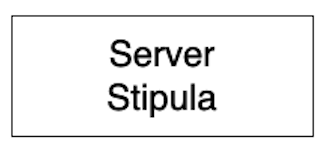
\includegraphics[width=0.3\textwidth]{immagini/capitolo-4/server-stipula.png}}
	\hspace{1cm}
	\subfloat[Example of an instance of a \textit{Stipula} server that relies on a blockchain.]
	{\label{fig:server-stipula-with-commitment}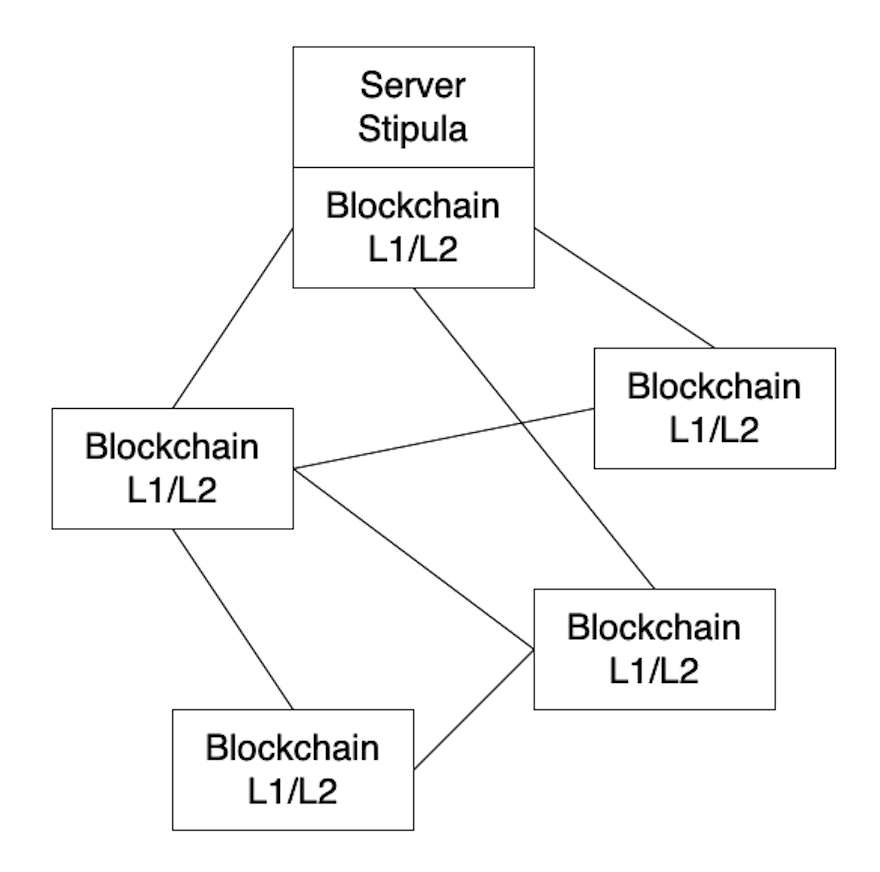
\includegraphics[width=0.4\textwidth]{immagini/capitolo-4/server-stipula-with-commitment.png}}\\
	\subfloat[Example of a network of \textit{Stipula} nodes.]
	{\label{fig:stipula-nodes}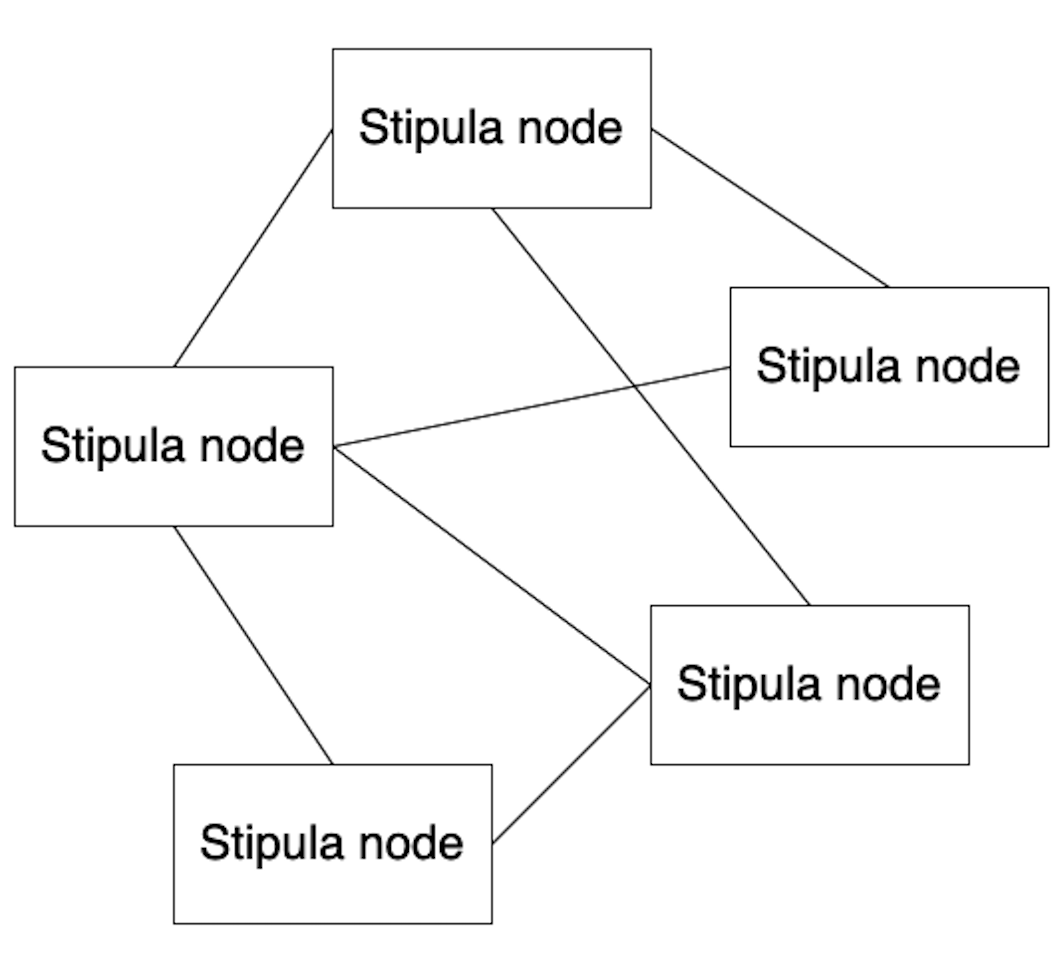
\includegraphics[width=0.4\textwidth]{immagini/capitolo-4/stipula-nodes.png}}
	\hspace{1cm}
	\subfloat[Example of a network of \textit{Stipula} nodes based on a blockchain.]
	{\label{fig:stipula-nodes-with-commitment}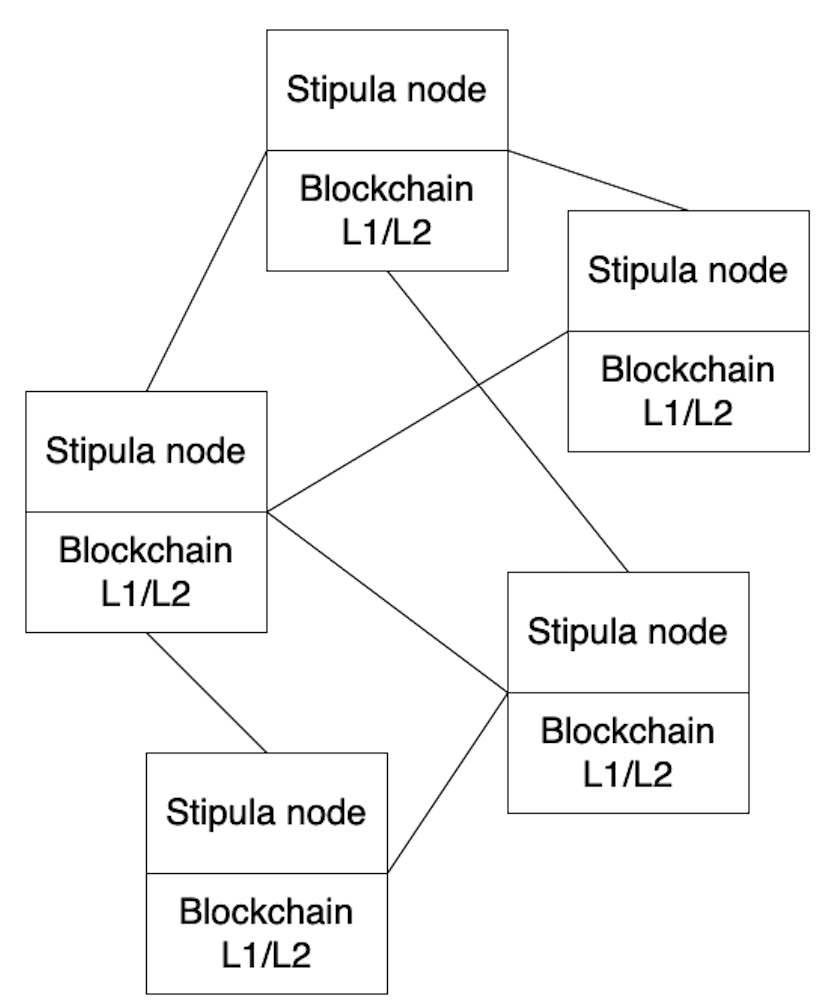
\includegraphics[width=0.4\textwidth]{immagini/capitolo-4/stipula-nodes-with-commitment.png}}
	\caption{Possible configurations of the \textit{Stipula} architecture.}
	\label{fig:network-configs}
\end{figure}

\newpage
\section{Architecture}

The main modules that make up the implementation architecture of the \textit{Stipula} language are
(\ref{fig:complete-architecture}):
\begin{enumerate}
	\item \textit{Message Service}: manages connection and communication with clients;
	\item \textit{Compiler}: receives as input a contract written in the \textit{Stipula} language and 
	compiles it in another language, called \textit{Stipula bytecode};
	\item \textit{Virtual Machine}: execute the code in \textit{Stipula bytecode} received as input;
	\item \textit{Consensus}: implements mechanisms that make it possible to determine consensus regarding the 
	result of executing a contract, within a network of nodes;
	\item \textit{Storage}: stores information about \textit{assets} and its \textit{transfers}, 
	\textit{contracts} and its \textit{instances};
	\item \textit{Commitment}: deals with communicating with the layer that allows you to securely store some 
	of the information stored in the \textit{storage} layer. At this level, it is not necessary to save 
	exactly all the information stored in the storage, it is sufficient to save a minimum set of such 
	information;
	\item \textit{Communication protocols}: implements a series of protocols necessary for the consensus layer 
	and for communication between nodes (i.e. \textit{node discovery}).
\end{enumerate}

\begin{figure}[htbp]
	\begin{center}
		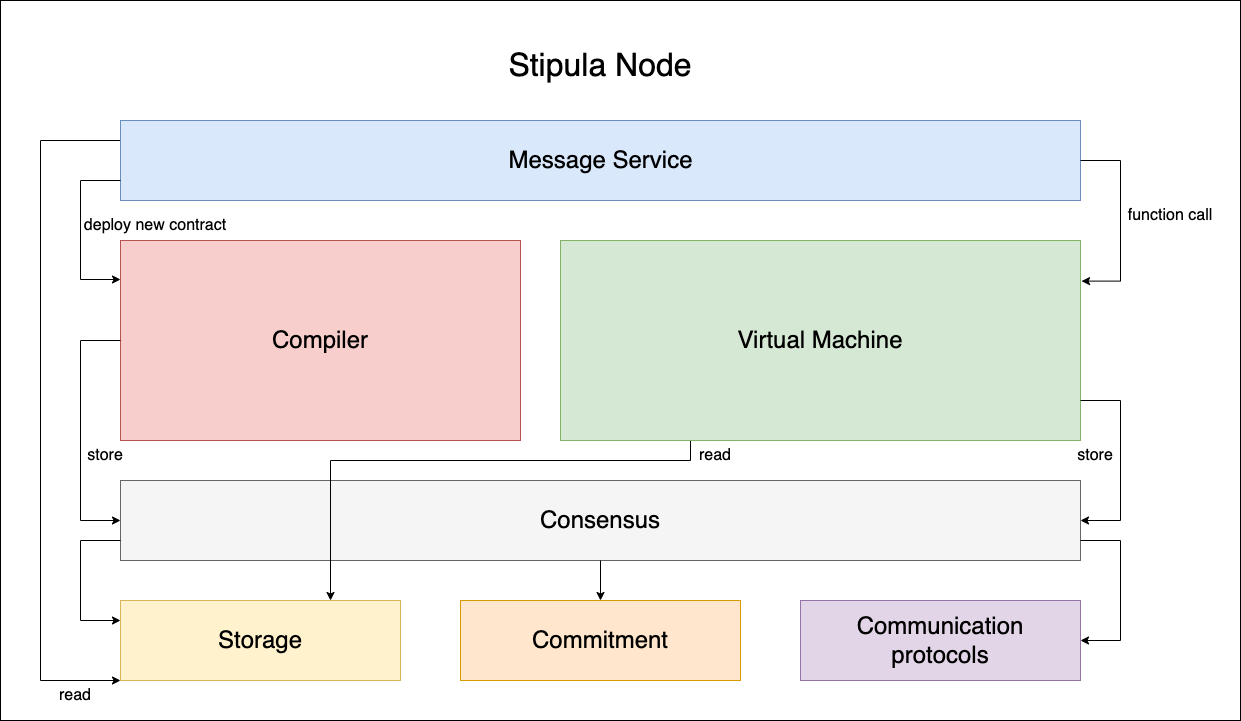
\includegraphics[height=7cm]{immagini/capitolo-4/complete-architecture.png}
		\caption{Complete architecture of all modules and interactions between them.}
		\label{fig:complete-architecture}
	\end{center}
\end{figure}

\newpage
\subsection{Message Service}

This module performs the role of \textit{server}, that is, it waits for new connections from clients. It was 
decided to use a TCP connection instead of HTTP for the following reasons:
\begin{enumerate}
	\item In order to communicate via the HTTP protocol, a \textit{web server} must be added to the 
	implementation. This would have weighed down the implementation and would not have made use of all the 
	features offered by the HTTP protocol;
	\item The TCP protocol is a \textit{reliable} and \textit{connection-oriented} protocol, that is, it frees 
	the application from the task of handling out-of-order or missing packets;
	\item The TCP protocol allows you to send and receive streams of bytes directly, instead of streams of 
	characters as is the case with the HTTP protocol. By doing so, you also get an advantage in terms of 
	efficiency.
\end{enumerate}

Once a new connection has been received from a client, the management of communication with that client is 
delegated to a \textit{thread}, in order to free up the server thread to accept new requests. Once the 
message sent by the client has been received and decoded, we proceed to check the \textit{signatures} of 
the message itself. Every message that is sent must be signed with the private key held by the client. If 
the signature check passes, then the request will be routed to other modules. The connection with the client 
remains open until the module to which the request was directed returns a response; once the response is 
received, it is sent to the client and the connection is closed.

\subsection{Compiler}

A \href[]{https://github.com/stipula-language/stipula}{first implementation} of the \textit{Stipula} language 
has been done previously. In this implementation, the language is \textit{interpreted} at \textit{runtime} 
and is executed locally on the machine. This approach has limitations if you want to translate it into the 
distributed context. Interpretation has the advantage of directly executing the code, without performing 
intermediate compilation steps. However, it has major drawbacks:
\begin{enumerate}
	\item \textit{Slow to execute}: the code is translated directly into machine code. An intermediate 
	compilation step could have optimized the code before running it;
	\item \textit{Low performance}: since the code is not optimized for the platform on which it runs;
	\item \textit{Less error checking}: this represents one of the weakest points of this approach, 
	particularly in the context of writing and executing contracts that have legal value.
\end{enumerate}
	
To overcome the limitations of this first implementation, it was decided to divide the process of executing a 
contract into two main steps:
\begin{enumerate}
	\item \textit{Compilation}: having received the contract as input, it is compiled in an intermediate 
	language called \textit{Stipula bytecode}. The characteristics of this language will be extensively 
	discussed in the following chapter;
	\item \textit{Execution}: having received the contract compiled in bytecode as input, this is executed.
\end{enumerate}

In this way we obtain an optimization in terms of performance, that is, once the contract has been compiled, 
the same contract can be called numerous times, without having to re-compile each time. Furthermore, having 
an intermediate compilation step it is possible to perform \textit{static} checks: it is possible to verify 
whether the contract states can actually be reached during execution, check if the asset transfers have been 
defined correctly and implement checks about the types of variables. As regards this last point, the 
\textit{Stipula} language is a \textit{weakly typed} language: when writing a contract it is possible to 
specify whether a variable is a \verb|asset| or is a \verb|field|. Obviously, if a variable is defined as 
\verb|field| it is necessary to perform a \textit{inference} operation to determine the specific type. 
However, it's not always possible to determine the type of a variable at compile time, so you need to 
determine it at runtime. 

The use of the bytecode language also allows you to obtain an advantage from the point of view of 
\textit{interoperability}. In fact, further compilers could be developed, which from other smart contract 
languages (i.e., Solidity), translate the smart contracts into \textit{Stipula bytecode} language.

\subsection{Virtual Machine}

The compilation phase produces code written in a particular language, specifically defined for the purpose 
of the project. Therefore, you need to build an environment for executing the contract bytecode. For this 
reason a \textit{virtual machine} has been developed. The benefits that follow from virtualization are:
\begin{enumerate}
	\item \textit{Platform independence}: the virtual machine creates an abstraction layer between the code 
	and the underlying hardware, thus allowing the code to be executed on different platforms, without the 
	need to recompile it every time;
	\item \textit{Secure environment}: the virtual machine creates a secure environment for execution, 
	especially needed for asset transfer.
\end{enumerate}

\label{stack-based-vm}
The virtual machine implemented is a \textit{stack-based virtual machine}, that is, the program variables 
are loaded onto a stack and the language instructions operate on that stack by removing or adding elements 
to the stack. A stack-based virtual machine is simpler to implement and requires fewer instructions to 
perform the same operations compared to a \textit{register-based} virtual machine. However, it must be 
taken into consideration that a stack-based virtual machine is less performing than a register-based 
virtual machine and also requires many more memory accesses. Aware of these differences, due to issues of 
time and complexity, it was decided to create a stack-based virtual machine.

The virtual machine manages various memory areas, as it must take into account the internal variables of 
the functions, the parameters of the functions and the global variables. In addition to these, there are 
also other memory areas whose purposes will be defined in the next chapter.

This module also takes care of managing the \textit{obligations}, that is, scheduling the events that will 
allow you to execute a specific portion of code, at a specific time. The management of this functionality 
involves both the compiler, in recognizing the obligation encoded in the code, and the virtual machine: 
during the execution of the contract, the scheduling request of an obligation is managed ad-hoc by a 
specific component of the virtual machine.

\subsection{Consensus}

Consensus is an essential component for the proper functioning of peer-to-peer networks, as it allows 
multiple nodes to agree on a single \textit{result}, even in the presence of failures. Without consensus, 
peer-to-peer networks would be prone to conflicts, inconsistencies, and vulnerabilities, making them less 
reliable and less secure. In a distributed context, multiple nodes work together to perform a task and 
must communicate with each other to exchange information and coordinate their actions. However, due to 
factors such as network delays, failures and communication errors, different nodes may have different 
views of system status (such as a contract or a transfer) or may produce conflicting results. In 
particular, the goals of consensus algorithms must guarantee:
\begin{enumerate}
	\item \textbf{Data consistency}: in a distributed ledger, multiple nodes can contain different copies of 
	the same data. Consensus algorithms ensure that nodes agree on a single version of the data, ensuring 
	data consistency and avoiding data corruption;
	\item \textbf{Fault tolerance}: nodes can fail or become unresponsive. The consent algorithms allow the 
	system to continue to operate even in the presence of node failures;
	\item \textbf{Conflict-free}: consensus algorithms ensure that the system is conflict-free, ensuring that 
	nodes agree on a single result;
	\item \textbf{Security}: Consensus algorithms can help prevent malicious actors from manipulating the 
	system by ensuring that all nodes agree on a single decision value, even in the presence of attacks such 
	as data tampering or \textit{Denial-of-Service} (\textit{DoS}).
\end{enumerate}

Therefore, the evolution of the status of a contract or the successful transfer of a certain amount of 
assets towards an address must be in agreement with the other nodes making up the network.

\subsection{Storage}
\label{storage-module}

This module takes care of storing various information regarding assets and contracts. In particular, 
information concerning:
\begin{enumerate}
	\item \textbf{Asset}: it is necessary to memorize information that characterizes the asset itself, such 
	as the name, a unique identifier, the total \textit{supply} and whether the asset is divisible or not. 
	Total supply is the total amount of asset that will be available for a specific asset;
	\item \textbf{Transfer of assets}: it is necessary to trace the movements of assets that are carried out 
	by customers and contracts. Later it will be explained in detail how asset transfers occur in the current 
	implementation;
	\item \textbf{Contracts}: the new contracts are loaded into a \textit{Stipula server} or a 
	\textit{Stipula node} and stored together with the bytecode produced by the compilation phase. Once a 
	contract is uploaded, it is no longer possible to make any changes;
	\item \textbf{Contract instances}: when you want to execute a contract, a new \textit{contract instance} 
	is created. The storage keeps track of \textit{each running contract instance}, together with its 
	\textit{current state}. For instance, two actors, Alice and Bob, want to activate an instance of BikeRental 
	with ItalyRent (see section \ref{bike-rental-example-definition}). There can be a BikeRental between Alice 
	and ItalyRent in state \verb|@Using|, and a BikeRental between Bob and ItalyRent in state \verb|@Return|.
\end{enumerate}

\subsection{Commitment}
\label{commitment-module}

For the context created by the proposed implementation, the commitment module represents the level at which 
information can be securely stored. Indeed, the purpose of this component is to offer a high level of security 
for the recording of information. It is not necessary to memorize all the information that is saved in the 
\textit{Storage} module, but a \textit{minimal} set of key information allows to reconstruct the evolution of 
the contract and of the asset transfers that have taken place over time. Thus, the commitment module is used to 
\textit{timestamping} the information, proving the \textit{existence} of a particular piece of information. The 
presence of this module within the implementation is not strictly necessary for the functioning of a 
\textit{Stipula} server or node, but it allows it to offer a higher level of security. As an example: we can 
devise a simple client-server implementation where the storage in managed by the server as an internal database, 
or a richer implementation where the server commits to a blockchain part of the storage to notarize the main 
info of the contract execution.

\subsection{Communication protocols}
\label{communication-protocols-module}

In a distributed context, it is necessary that the various nodes can communicate with each other to exchange 
information. The type of information exchanged can be divided into:
\begin{enumerate}
	\item Information to determine \textit{consent} about the status of a contract;
	\item Information to manage \textit{connections} with other nodes (i.e., discovery of new nodes, notify 
	that a node is congested, \dots).
\end{enumerate}

The design of a communication protocol is critical because it determines how efficiently and accurately 
information is transmitted and received. Poorly designed protocols can cause a variety of problems, such as 
slow performance, lost or corrupted data, security vulnerabilities, and difficulties in scalability and 
maintainability.

\section{Interaction between modules}

In this section we want to explain how the interactions between the various modules of the architecture take 
place. Each request sent by a client is received by the \textit{Message Service} module, which, after 
carrying out the appropriate checks, can direct the request towards different modules according to the 
specific request:
\begin{enumerate}
	\item Towards the \textit{Compiler}: when the request received represents the user's will to load a new 
	contract. The contract is received from this module, which proceeds with the compilation of the same;
	\item Towards the \textit{Virtual Machine}: when with this request the client wants to create a new 
	instance or perform a function of a specific contract instance.
	\item Towards the \textit{Storage}: when the client's request consists in a reading of some information 
	(i.e., available assets associated with its address).
\end{enumerate}

It is necessary to specify that all the requests that are addressed to the \textit{Storage} module are 
always read requests and never write requests; writing information can only be done for compiling a new 
contract (\textit{Compiler}) or for running an instance of a contract (\textit{Virtual Machine}).

If the request is of type ($1$) or of type ($2$), the results produced by the respective modules are routed 
to the consent module. The reason is that before writing any information to the storage and/or commitment 
layer, the network must agree on the same information to be written. Consequently, this phase also involves 
the module that implements all the communication protocols between the nodes, since, in order to be able to 
determine consensus within the network, the nodes must be able to communicate with each other. Furthermore, 
this module will carry out activities regardless of the requests received from the clients, in fact within 
this part of software there are also the protocols that allow you to manage the connections with the other 
nodes.

\section{Asset management}

The language offers primitives that allow you to handle the transfer of assets carefully and independently 
of how the assets are actually implemented. These design choices made the language very clear to write and 
read code.

\subsection{Definition of assets}
\label{asset-definition}

One of the most important points of the development of this thesis project concerns the provision of an 
implementation of the concept of \textit{asset}. As a basic idea, it was decided to try to reproduce the 
same characteristics of blockchain \textit{token} such as \textit{Ethereum} or \textit{Algorand}, adapting 
the complexity to the current development of the project. Thus, the main characteristics of an asset are:
\begin{enumerate}
	\item \textbf{Unique identifier}: consists of an alphanumeric string to uniquely refer to an asset;
	\item \textbf{Name of the asset}: a name is defined that can be easily remembered by a person;
	\item \textbf{Unit name}: corresponds to what is a \textit{ticker} of a company listed on the stock 
	exchange (i.e., APPL for Apple company);
	\item \textbf{Decimals}: indicates how many parts a single unit can consist of;
	\item \textbf{Maximum supply}: indicates the maximum amount of assets that can exist over time. The 
	maximum quantity also includes decimal values, for example: if you want to define an asset 
	\verb|StipulaCoin| which can only have 10 units and each unit can be divided into 100 sub-units, therefore 
	the maximum supply will be 1000 sub-units.
\end{enumerate}
Example of definition of an hypothetical \verb|StipulaCoin| asset:
\label{definition-fungible-asset}
\begin{enumerate}
	\item \textit{Unique identifier}: \verb|stipula_coin_asd345|
	\item \textit{Name of the asset}: \verb|StipulaCoin|
	\item \textit{Unit name}: \verb|STC|
	\item \textit{Decimals}: 3
	\item \textit{Maximum supply}: 1000
\end{enumerate}
The \verb|StipulaCoin| asset thus defined has an identifier (\verb|stipula_coin_asd345|), a unit name 
(\verb|STC|), has a maximum supply of 1000 sub-units and the number of decimals is equal to 3, so a single 
unit can be divided into 100 sub-units.

With this structure it is possible to define different types of assets, such as:
\begin{enumerate}
	\item \textbf{Fungible assets} (i.e., bitcoins and banknotes): an asset is fungible when it is 
	\textit{interchangeable} from the point of view of the units that compose it, i.e., that each of its units 
	is \textit{indistinguishable} the from each other, for the same nominal value. It is possible to define 
	both divisible and non-divisible fungible assets;
	\item \textbf{Non-fungible assets} (i.e., NFT): contrary to fungibility, the units that make up the asset 
	are unique and therefore are not interchangeable with each other. Furthermore, another feature that 
	distinguishes them from fungible assets is that they are not divisible.
\end{enumerate}

An example of a fungible asset was shown above (\ref{definition-fungible-asset}). An example of a 
non-fungible asset is provided:
\begin{enumerate}
	\item \textit{Unique identifier}: \verb|stipula_nft_abc123|
	\item \textit{Name of the asset}: \verb|StipulaNFT|
	\item \textit{Unit name}: \verb|SNFT|
	\item \textit{Decimals}: 0
	\item \textit{Maximum supply}: 1
\end{enumerate}
The \verb|StipulaNFT| asset thus defined has an identifier (\verb|stipula_nft_abc123|), a unit name 
(\verb|SNFT|), has a maximum supply of 1 unit and the number of decimals is equal to 0, because a 
non-fungible asset cannot be split.

However, the definition of the characteristics of an asset is not sufficient to also define in which 
\textit{way} the assets are transferred. Therefore in the next section we will proceed to provide a 
possible solution for asset transfer.

\subsection{Transfer of assets}

The way in which the transfer of assets is implemented represents one of the most delicate points of the 
whole project. When you want to send a certain amount of a specific asset, you want to guarantee some 
properties:
\begin{enumerate}
	\item \textbf{Atomicity}: the transaction must take place atomically from the sender to the recipient;
	\item \textbf{Consistency in the quantity transferred}: we want to ensure that no quantities of assets 
	are lost or quantities of assets are generated out of nothing, during a transaction;
	\item \textbf{Prevent assets from getting stuck}: you want to prevent assets from getting stuck in 
	contracts, and therefore cannot be spent;
	\item \textbf{Proof of possession}: you want to have proof that the amount of assets you want to move is 
	actually owned by the sender;
	\item \textbf{Avoid double-spending}: prevent an entity from being able to pay two recipients using 
	exactly the same amount of assets. This is a problem that does not arise with, for example, banknotes, 
	but it is a problem that affects digital assets. This problem is due to the fact that in the digital 
	context, unlike the real world, it is difficult to reproduce the concept of \textit{scarcity} of a good.
\end{enumerate}

The problems indicated in points ($1$) and ($3$) are totally solved by the \textit{Virtual Machine} 
(see section \ref{virtual-machine}), however, the check that during the transfer of assets no amount of 
assets is lost or generated, is only solved partially (see sections \ref{asset-implementation} and 
\ref{script-vm}). The solution to the other points will be explained later in sections 
\ref{asset-implementation} and \ref{virtual-machine}.

\subsubsection{Pay-to-Contract and Pay-to-Party}
\label{pay-to-contract-and-pay-to-party}

Blockchains like \textit{Ethereum} or \textit{Algorand} allow you to send and receive coins without using 
contracts and to exchange tokens using smart contracts. In the current implementation for \textit{Stipula}, 
it is not possible for two entities to exchange assets except through a contract. This is because it would 
have required the development of primitives external to the virtual machine in order to enable the transfer 
of assets without going through a contract. The purpose of the implementation is to build a platform for the 
execution of legal contracts, and not to create a platform for pure asset transaction.

Taking into account that any transfer of assets must take place through the execution of a contract, it is 
necessary to define how these transfers must take place between the participants of a contract. Each 
\textit{party} of a contract (that is, the participants of the contract) owns a pair of 
\textit{cryptographic keys}, with which it is able to send signed messages and to prove possession of 
certain properties. A party, not being able to directly send assets to another party, must send these assets 
to the contract. This operation is defined as \textbf{Pay-to-Contract} or \textbf{deposit}, i.e., when the 
party makes a function call that requires sending a certain amount of assets, it sends it to the contract. 
In the execution phase of the function call, all the necessary checks will be performed to verify that the 
party is actually the owner of that amount of assets. Once the checks have been carried out, it will now be 
the contract that guarantees the integrity of the assets, i.e., thanks to the definition of the language 
primitives, it will be the contract that ensures that no quantities of assets will be lost into thin air or 
quantities of assets will be generated from nothing . Instead, the operation that occurs when the contract 
has to send assets to a party is called \textbf{Pay-to-Party} or \textbf{withdrawal}. Again, the language 
primitives will ensure that the party will receive the correct amount of assets. Thus defining the deposit 
of assets in a contract and the withdrawal of assets from a contract, it is possible to transfer assets 
between two or more parties by means of a contract, without the need to implement additional primitives 
external to the language and specific to the implementation of the architecture. A simple example that 
illustrates how \textit{Pay-to-Contract} and \textit{Pay-to-Party} work is shown in the example in section 
\ref{asset-swap}, where two actors, Alice and Bob, exchange two assets with each other.

\subsubsection{Single-use-seals}
\label{single-use-seal-definition}

Despite the definition of an asset management structure and the definition of the operations to send and 
receive assets, the definition of a model to represent and manage the balances of various assets that a 
party can have is missing. The simplest model to implement is the \textbf{account-balance-based} model, 
where each address has a balance associated with it. With each transaction, the balance of the sent asset is 
updated, both for the sender and for the recipient. An example of an account-balance-based model:
\begin{Verbatim}[numbers=left,xleftmargin=2cm]
	...
	"partyA": {
		"asset1": {
			"balance": 123.65
		},
		"asset2": {
			"balance": 18.44
		}
	}
	...
\end{Verbatim}

However, this simple model has problems in terms of:
\begin{enumerate}
	\item \textit{Scalability}: if you want to send two transactions of an asset \verb|asset1|, these 
	transactions cannot be parallelized, as the second transaction must wait for the balance of asset 
	\verb|asset1| is updated for the sender and the recipient after the execution of the first transaction;
	\item \textit{Privacy}: it is a model that allows you to very easily track the funds associated with an 
	address.
\end{enumerate}

An alternative model has been introduced by Bitcoin: the \textbf{Unspent Transaction Output} (\textbf{UTXO}) 
model. It is a more complex model than the previous one but offers advantages in terms of scalability, 
privacy and security. To give a concrete example, we can define a UTXO as a box that contains a certain 
amount of an asset. This box is closed by a \textit{single-use-seal} which can only be broken by the owner 
of the quantity of assets in question. To explain how this model works, we introduce the following example: 
suppose Alice has to give Bob 1 \verb|StipulaCoin|. Alice owns two UTXOs, \verb|UTXO_1| and \verb|UTXO_2|, 
each of 1 \verb|StipulaCoin|. At this point, Alice chooses to use \verb|UTXO_1|, she breaks the seal and 
creates a new seal so that only Bob can then break it in turn. By doing so, \verb|UTXO_1| it becomes Bob's 
property and only he can spend it in future transactions. The breaking of the seal can only be done if the 
user is able to provide cryptographic proof that he is the rightful owner of the UTXO. The balance of Alice 
and Bob's \textbf{wallets} are given by the sum of the UTXOs in their possession: before the transaction, 
Alice had 2 \verb|StipulaCoin| contained in two different UTXOs, that is, \textit{two transaction outputs 
(received) not (yet) spent}, while Bob had 0 \verb|StipulaCoin|; after the transaction, Alice has 1 
\verb|StipulaCoin| and Bob has 1 \verb|StipulaCoin| (the one received from Alice), that is, both have 
\textit{an output of a transaction (received) not (yet) spent}.

The advantages of using this model are:
\begin{enumerate}
	\item \textit{Parallelization}\label{utxo-parallelization}: unlike the account-balance-based model, 
	transactions that correspond to two payments using two different UTXOs can be parallelized, without having 
	to wait for the balance to be updated of the transacted asset after the first transaction. Taking the 
	above example, Alice could send \verb|UTXO_1| to Bob with a transaction and send \verb|UTXO_2| at the same 
	time Charlie;
	\item Partially solves the \textit{double-spending} problem: a specific UTXO can be spent on only one 
	transaction and not on others. The problem is partially solved because the network of nodes still has to 
	verify that a user does not try to pay multiple transactions with the same UTXO;
	\item \textit{Security}: in order to spend funds, cryptographic proof of ownership of the assets to be 
	moved must be provided;
	\item \textit{Privacy}: this model encourages not to reuse the same addresses, making it more difficult 
	to trace funds. In fact, each transaction accepts UTXO as input and generates new UTXO as output. If the 
	same address is used over and over again to make payments, it becomes easier for an observer to track the 
	history of transactions associated with that address, potentially revealing sensitive information;
	\item \textbf{UTXO selection}\label{coin-selection}: consists of the process of choosing the UTXOs, from 
	the set of available UTXOs, to cover the transaction amount while minimizing the transaction fees in 
	Bitcoin. If you select UTXOs with a large value, you may pay higher transaction fees than if you selected 
	UTXOs with a smaller value. Also, if you select too many UTXOs to cover your transaction amount, you may 
	find yourself having a larger transaction size, which can also result in higher fees. Introduce the 
	following example to clarify the implications of this technique: suppose you want to send someone 0.5 
	\verb|StipulaCoin| and that you have several UTXOs in your wallet, including:
	\begin{itemize}
		\item 1 \verb|StipulaCoin|
		\item 0.7 \verb|StipulaCoin|
		\item 0.5 \verb|StipulaCoin|
		\item 0.2 \verb|StipulaCoin|
	\end{itemize}

If you select the UTXO from 1 \verb|StipulaCoin| to complete the transaction, you will end up paying a 
higher commission than if you selected the 0.5 UTXO \verb|StipulaCoin|. This is because the transaction 
size for the UTXO is 1 \verb|StipulaCoin| is greater than that of the 0.5 \verb|StipulaCoin| UTXO, which 
means that it will cost more to include in a block. Therefore, selecting the appropriate UTXOs for a 
transaction is important to minimize fees and ensure that the transaction is processed quickly and 
efficiently.
\end{enumerate}

For the implementation of the \textit{Stipula} language, it was decided to pay greater attention to network 
security (avoiding double-spending), user security (verifying ownership of funds through cryptography) and 
privacy. Hence, it was decided to implement a model similar to that of Bitcoin. The implemented 
model representation is much simpler than that of a UTXO, therefore to keep separate the original concept 
from the one implemented for the thesis, it was decided to use a different name: \textbf{single-use-seal}. 
This term wants to refer in particular to the key action that occurs during a transaction, i.e. the breaking 
of the seal by the sender and the creation of a new seal that only the recipient will be able to break in 
turn. This step represents the \textit{transfer of ownership} of a certain amount of assets from one user to 
another.

\subsubsection{Script}
\label{script-language}

The \textit{smart contract} concept was first proposed by cryptographer Nick Szabo 
\autocite{site:smart-contract-szabo}. Szabo described smart contracts as computer protocols that facilitate, 
verify, or enforce the negotiation or performance of contractual obligations, without the need for a trusted 
third party. However, it was only with the development of blockchains that smart contracts became practical to 
implement. The first blockchain-based platform where it was possible to create and execute smart contracts was 
Ethereum. This blockchain introduced a programming language called \textit{Solidity}, which allows developers 
to write smart contracts and deploy them on the blockchain.

Before Ethereum, the first large-scale application of the smart contract concept was Bitcoin with the 
implementation of the \textbf{Script} language. It is a \textit{stack-based} language and offers a flexible 
and secure way to define the conditions under which a transaction can be spent in the Bitcoin network, 
enabling more advanced transaction types, such as requiring more signatures or a certain amount of time 
before that the funds can be transferred. These rules can be combined in different ways to create more 
complex transaction types and smart contracts. For example, a transaction with multiple signatures might 
require approval from multiple parties before funds can be transferred, while a time-locked transaction 
might require a certain amount of time before funds can be accessed.

In the previous section we introduced \textit{UTXO} and its simplified version, \textit{single-use-seals}. 
When a user has to pay for a contract, he has to provide cryptographic proof of ownership of the 
single-use-seal. The naive solution is to send a message representing the call of a function, within which 
the cryptographic demonstration is provided. The cryptographic proof can consist in signing the 
single-use-seal identifier with the private key, so that the user can prove possession of it. However, 
this solution is very limited: if you wanted to implement a payment that requires approval from different 
users, you would have to update the message format or create a new message type (i.e., update the 
\verb|FunctionCall| message in order to collect more signatures). To avoid having to create many different 
message formats, it is possible to encode the cryptographic proof as a contract written in \textit{Script}. 
By doing so, the cryptographic proof can be represented by a complex contract written in \textit{Script} 
and which will be validated to verify if:
\begin{enumerate}
	\item The program is syntactically and semantically correct, and
	\item The signatures collected are correct and the conditions imposed by the contract have been respected.
\end{enumerate}

Szabo's smart contract idea is different from \textit{Stipula}'s legal contracts. \textit{Script} allows you 
to manage the expenditure of funds in a secure and advanced way, \textit{Stipula} takes care of executing 
programs that codify specific contractual obligations. The two languages have two different purposes and 
therefore can coexist in the same implementation. In fact, a language similar to \textit{Script} was used 
to manage asset transfers and whose programs are executed by a specific component of the virtual machine. 
Thus, the \textit{Virtual Machine} module allows both to execute contracts in \textit{Stipula} and contracts 
in \textit{Script}. By analogy with the language used in Bitcoin, it was decided not to change the name of 
this language, as they share the same instructions and mechanisms. All the details of how the 
\textit{Script} language works will be described later.

\subsubsection{Fungibility of assets and non-fungibility of single-use-seals}

In the \ref{asset-definition} section, the difference between fungibility and non-fungibility has been 
defined. It should be noted that a UTXO or single-use-seal \textit{is not fungible}. This is a property that 
both UTXO and single-use-seals have in common, so during the explanation we will refer to UTXO for the sake 
of brevity. A UTXO is non-fungible as it represents the value (quantity of assets) of a specific output 
obtained from a specific transaction. Once a UTXO is spent in a transaction, this UTXO is \textit{consumed}, 
and therefore can not \textit{never} be used again for a future payment. Also, a UTXO cannot be split, that 
is, you cannot break the seal, take a fraction of the amount of assets it contains, and put the same seal 
back on. If Alice has to send 2 \verb|StipulaCoin| to Bob but she only has a UTXO of 5 \verb|StipulaCoin|, 
the following actions will happen:
\begin{enumerate}
	\item Alice provides cryptographic proof that she owns the UTXO containing 5 \verb|StipulaCoin|, so she 
	breaks the seal for that UTXO;
	\item Alice prepares two new UTXOs: one of 2 \verb|StipulaCoin| with a seal that only Bob can break, and 
	a 3 \verb|StipulaCoin| UTXO with a seal that only Alice can break. The latter UTXO represents the 
	\textit{remainder} of a transaction. A similar situation can be encountered when using banknotes: if you have a banknote whose value exceeds that of the item you want to buy, the seller will withhold the amount equal to the value of the item and return it to the buyer the difference.
\end{enumerate}

The non-fungibility of UTXOs is important because it ensures that each transaction is recorded as a unique 
event, with a specific sender, recipient and value. This provides a high level of transparency and security, 
as it is difficult to manipulate transaction history. Also, since UTXOs cannot be reused, it reduces the 
risk of double-spending and makes it easier to track the movement of funds. However, it also means that it 
can be more difficult to make small or precise transactions, as UTXOs must be screened in their entirety.

\subsubsection{Difference from Ethereum}

When a user wants to interact with a smart contract on Ethereum, the user must authorize it to access their 
funds. By doing so, the contract will be able to spend funds in your name. This practice is called 
\textit{token allowance}. This feature represents a serious weakness regarding the security of funds. 
Indeed, there have been several cases of users approving malicious contracts with the aim of exfiltrating all 
possible funds. The philosophy which has been pursued for the implementation of the \textit{Stipula} 
language, and which has already been introduced previously, consists in giving the user full control over 
his own funds. When a user wants to make a function call of a specific \textit{Stipula} contract that 
requires the sending of a certain amount of assets, the user cryptographically proves ownership of the 
single-use-seal to be sent and transfers ownership to the contract. Now that the funds belong to the 
contract, the latter will be able to manage them adequately according to the defined rules. A contract 
\textit{Stipula} can never embezzle users' funds without their explicit permission. Obviously, this approach 
has the disadvantage for the user of having to sign several transactions if the contract requires it. 
Instead, in Ethereum, thanks to the token allowance, the smart contract can carry out several transactions, 
without having to ask the user to sign them each time. The proposed solutions are orthogonal to each other 
and it was decided to always aim to ensure a higher level of security, to the detriment of a limitation of 
the functions that can be offered.
             % Design
% !TEX encoding = UTF-8
% !TEX TS-program = pdflatex
% !TEX root = ../tesi.tex

%**************************************************************
\chapter{Implementation}
\label{cap:implementation}
%**************************************************************.

In the previous chapter the general architecture of the project was introduced (figure 
\ref{fig:complete-architecture}). However, the current version is a simplified version of the initial 
architecture. In particular, the current architecture is illustrated in figure 
\ref{fig:current-architecture}. The implemented architecture consists of a Java application, usable 
remotely via socket communication. All interactions with this architecture take place according to the 
classic \textit{client-server} model. The reason for this simplification is mainly due to the complexity 
of developing components, such as the \textit{Virtual Machine}, the compiler and the asset management 
model (\textit{single-use-seals}). However, the design of this architecture also takes into account future 
developments, which will be illustrated in the next chapter. The current architecture represents a 
starting point for the realization of the architecture presented in the previous chapter.

\begin{figure}[htbp]
	\begin{center}
		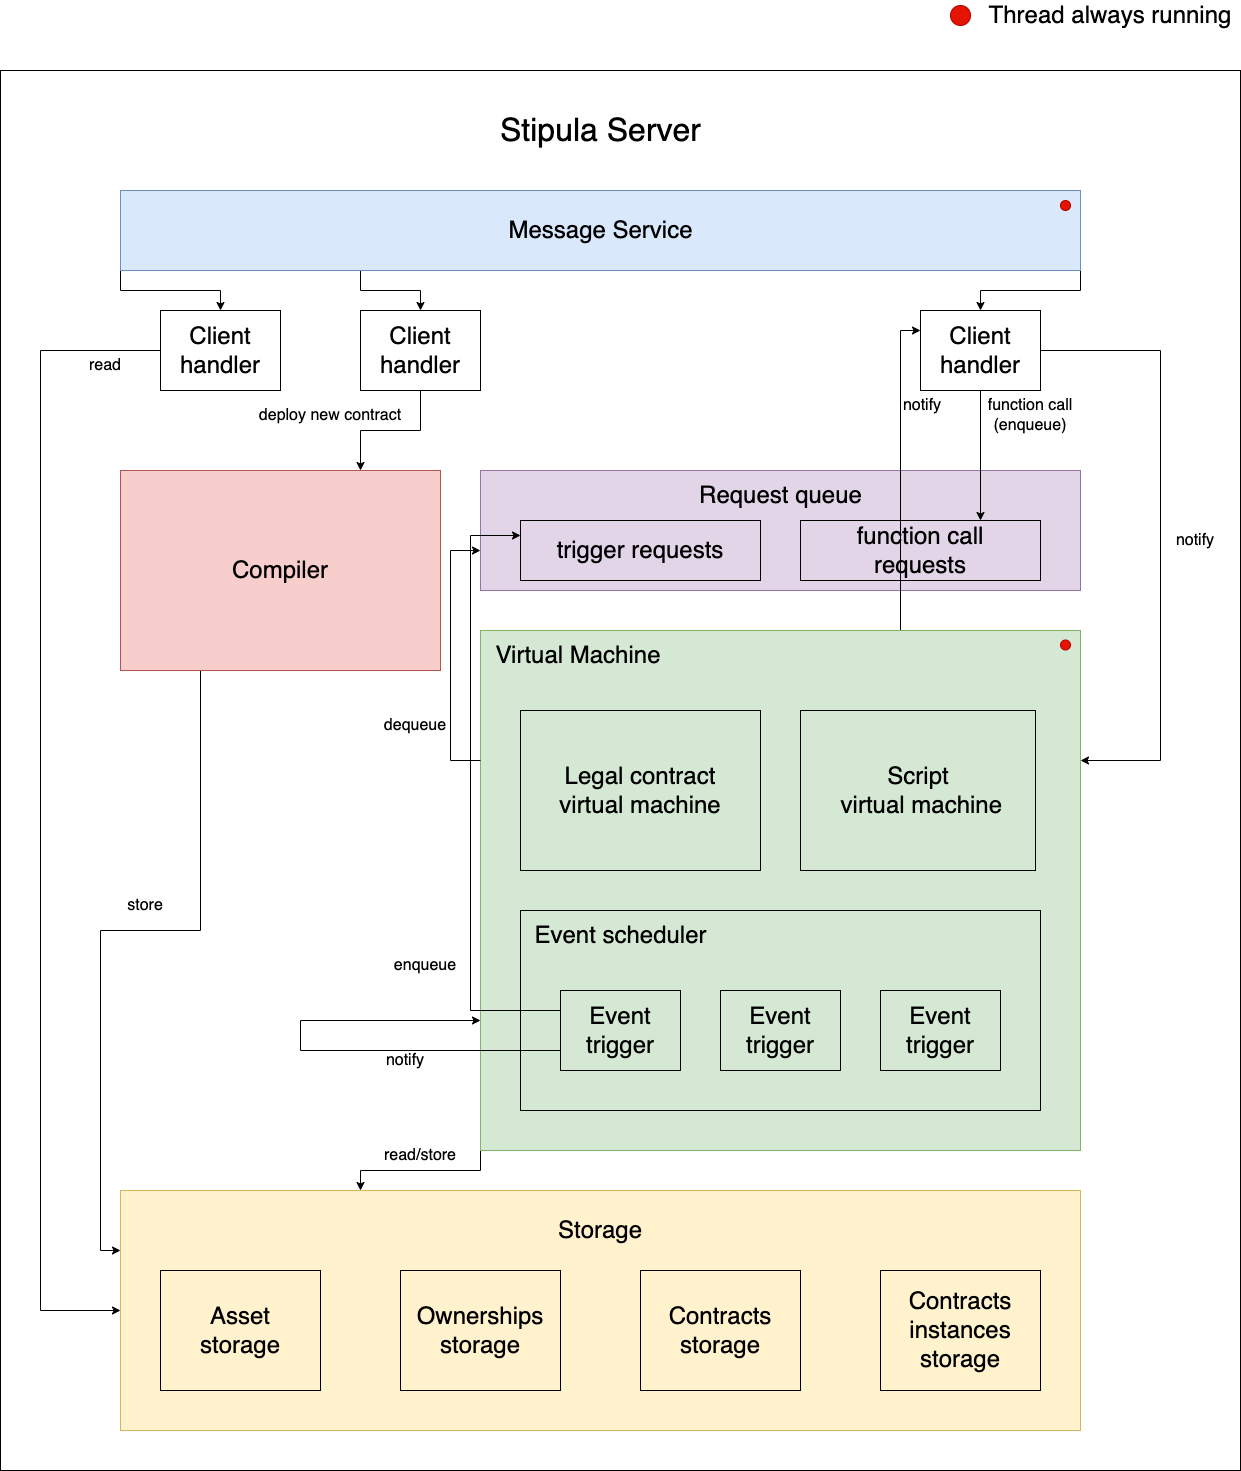
\includegraphics[width=0.9\textwidth]{immagini/capitolo-5/current-architecture.png}
		\caption{Current state of the implemented architecture.}
		\label{fig:current-architecture}
	\end{center}
\end{figure}

%**************************************************************

\section{Introduction to basic concepts}

The previous chapter introduced the concepts that form the basis on which the current architecture is 
based, such as assets and their management, and contracts. In this section these concepts will be analyzed 
from an implementation point of view, in order to help in understanding the functioning of the 
architecture in its complexity.

\subsection{Contracts and contract instances}
\label{contract-and-contract-instances-implementation}

In the current version of the architecture, there is a difference between a \textit{contract} and a 
\textit{instance of a contract}. The difference is similar to \textit{class} and \textit{object} (or 
\textit{instance of a class}) for object-oriented programming. When two actors want to \textit{execute} a 
contract, they will agree to create a new instance of a contract. The contract will be 
\textit{immutable}, while a contract instance can change over time.

From an implementation point of view, a contract is represented as follows:
\begin{enumerate}
  \item The source code of the contract;
  \item The compiled contract, that is, the bytecode;
  \item The initial state of the contract state machine;
  \item The final states of the contract state machine (optional);
  \item The contract state machine transitions.
\end{enumerate}

When this set of information is sent to the \textit{Storage} module, the latter generates an 
identification code to be associated with the contract. This identifier is sent in response to the client 
requesting to load the contract (see \ref{deploy-contract}). 

An instance of a contract is represented as follows:
\begin{enumerate}
   \item The \textbf{identifier of the contract}: it must be specified which specific contract you want 
   to refer to;
   \item The \textbf{participants of the contract};
   \item The definition of a \textbf{memory space} dedicated to maintaining the state of the global 
   variables during the evolution of the instance of the contract;
   \item A \textbf{state machine}: this structure is needed to track the progress of the contract 
   instance over time and to ensure that the contract participants operate without violating the 
   established order of operations.
\end{enumerate}

This distinction between contract and instance of a contract allows for the creation of multiple instances 
starting from the same contract, i.e., multiple users can use the same contract multiple times, present in 
a server or \textit{Stipula} node, creating multiple instances.

\subsection{Asset}

\subsubsection{Definition}
\label{asset-implementation}

As illustrated in the previous chapter (see \ref{asset-definition}), the goal is to try to reproduce the 
concept of \textit{token}, as is the case for Ethereum. An asset within the architecture is represented 
in Java by the object \verb|AssetConfig| class:
\begin{enumerate}
\item \verb|String assetName|: a name is defined that can be easily remembered by a person;
\item \verb|String unitName|: corresponds to what is a \textit{ticker} of a company listed on the stock 
exchange;
\item \verb|int decimals|: indicates how many parts a single unit can be in;
\item \verb|int supply|: indicates the maximum amount of assets that can exist over time.
\end{enumerate}

When this set of information is sent to the \textit{Storage} module, the latter generates an 
identification code to be associated with the asset. The object being stored contains the 
\verb|String id| fields and \verb|AssetConfig asset|.

At this point, creating \textit{fungible} and \textit{non-fungible} assets consists in extending the 
\verb|AssetConfig| class. In particular:
\begin{enumerate}
  \item 
  \begin{Verbatim}[numbers=left,xleftmargin=1cm,firstnumber=1,breaklines=true,breakanywhere=true,tabsize=2]
    public class FungibleAsset extends AssetConfig {
        public FungibleAsset(String assetName, String unitName, int supply, int decimals) {
            super(assetName, unitName, supply, decimals);
        }
    }
  \end{Verbatim}
  \item 
  \begin{Verbatim}[numbers=left,xleftmargin=1cm,firstnumber=1,breaklines=true,breakanywhere=true,tabsize=2]
    public class NonFungibleAsset extends AssetConfig {
        public NonFungibleAsset(String assetName, String unitName) {
            super(assetName, unitName, 1, 0);
        }
    }
  \end{Verbatim}
\end{enumerate}

\section{Libraries}
\label{libraries}

This package contains all the fundamental data structures for the overall development of the project. 
Furthermore, a library that implements cryptographic functions has been implemented.

\subsection{Crypto}

This library implements a number of cryptographic features, useful both for the architecture and for 
external software such as SDKs and wallets. The implemented methods are:
\begin{enumerate}
   \item \verb|generateKeyPair|: allows you to generate a 1024-bit RSA key pair;
   \item \verb|encrypt|: allows you to encrypt the received input;
   \item \verb|decrypt|: allows to decrypt the received input;
   \item \verb|getPublicKeyFromFile|: allows you to create a public key from a file;
   \item \verb|getPrivateKeyFromFile|: allows you to create a private key from a file;
   \item \verb|readKeyFromFile|: allows you to read a key from a file;
   \item \verb|getPublicKeyFromString|: allows you to create a public key from a string;
   \item \verb|sign|: allows you to sign the received input;
   \item \verb|verify|: allows you to verify if a signature is valid.
\end{enumerate}

\subsection{Data structures}

This package contains all the fundamental data structures for the implementation of the architecture. In 
particular, the data structures are:
\begin{enumerate}
   \item \verb|Pair|: represents a collection of two items of any type. The order of the elements is 
   important and allows two related values to be stored and manipulated as a single element;
   \item \verb|Triple|: it is a structure similar to the previous one, but it allows to manage three 
   elements;
   \item \verb|Queue|: is a data structure that implements the \textit{First-In-First-Out} 
   (\textit{FIFO}) policy, ie, the first item added to the queue is the first to be removed. This 
   structure is used when algorithms need to process a sequence of elements in a specific order;
   \item \verb|Stack|: is a data structure that implements the \textit{Last-In-First-Out} 
   (\textit{LIFO}) policy, i.e., the last element added to the stack is the first to be removed.
\end{enumerate}

In addition to these data structures, data structures provided directly by Java have been used, such as 
\textit{ArrayList} and \textit{HashMap}.

\section{Message Service}
\label{message-service}

This module is responsible for managing communication with clients, accepting their requests and 
redirecting them to the appropriate architecture modules. Before accepting requests, checks are carried 
out on the correct format of the message and the signatures associated with the message itself.

\subsection{MessageServer}

This component allows you to create an instance of a \textit{server}, which waits for new connections from 
\textit{clients}. When a new request arrives, the connection is delegated to a dedicated thread; by doing 
so, the server is ready to accept new connections. The other tasks of this component are to:
\begin{enumerate}
  \item Instruct the dedicated thread, passing it all the objects it needs;
  \item \label{shared-memory} Allocate a specific zone in \textbf{shared memory}. This memory zone is 
  shared between these threads and the virtual machine and is required for communication between these two 
  components. From the point of view of the implementation, shared memory is represented by one 
  \textit{map}, where the key is a string that serves as an identifier to access the cell, and the value 
  is a generic \verb|T| object.
\end{enumerate}

\subsection{ClientHandler}

This component takes care of managing a single connection with a client. In addition, this component takes 
care of:
\begin{enumerate}
   \item Check the \textit{signatures} of the message received from the client;
   \item If the previous check is successful, this component takes care of directing the request to the 
   correct module.
\end{enumerate}

When a response has been received from the module to which the request was directed, the 
\verb|ClientHandler| \textit{deallocate} the memory zone from shared memory.

\subsection{ClientConnection}

This component allows you to manage the connection more easily. In fact, it exposes high-level 
functionality, hiding certain complexities regarding socket management. This component allows you to make 
the \verb|ClientHandler| code more compact and readable.

\subsection{Messages}
\label{messages}

The messages currently in the implementation will be explained below. These represent the fundamental 
messages to allow the execution of the contracts. In the future, this ensemble will certainly be expanded. 
For ease of implementation, message transmission consists of direct encoding of Java objects in JSON 
format.

\subsubsection{DeployContract}
\label{deploy-contract}

This message allows you to load a new contract into the \textit{Stipula} instance. The only required value 
is the \textit{source code} of the contract. This request will then be routed to the compiler.

\subsubsection{FunctionCall}
\label{function-call-message}

This message allows you to make a function call for a specific instance of a contract. The required 
parameters are:
\begin{enumerate}
   \item \verb|contractInstanceId|: identifier of the instance of the contract to which it refers;
   \item \verb|functionName|: name of the function to call;
   \item \verb|arguments|: the list of arguments of the function to call. The elements of this list are 
   \textit{triples}. In this case, the meaning of a triple is \textit{variable type}, 
   \textit{variable name} and \textit{variable value}.
\end{enumerate}

This request will then be routed to the virtual machine.

\paragraph{Pay-to-Contract}
\label{pay-to-contract}

In the previous chapter the concept of \textit{Pay-to-Contract} was introduced (see 
\ref{pay-to-contract-and-pay-to-party}), that is, the user can make a payment to an instance of a 
contract, using one of its \textit{single-use-seals}. Previously, the \verb|FunctionCall| object was 
introduced, which allows you to supply the parameters of a specific function. These parameters are 
specified by the \verb|arguments| field, which is of type \verb|Triple<String, String, Object>|. The last 
component of the triple accepts a value of type \verb|String| or of type \verb|PayToContract|. This last 
object allows you to provide all the information necessary to make the payment to the contract instance. 
In particular, the fields of the object are:
\label{ownership}
\begin{enumerate}
   \item \verb|String ownershipId|: it is the identifier of the \textit{single-use-seal} that the user 
   wants to spend;
   \item \verb|String address|: the address of the owner of the \textit{single-use-seal};
   \item \verb|String unlockScript|: consists of a cryptographic proof proving that the user is the 
   effective owner of the \textit{single-use-seal}. The meaning of this field will be described later.
\end{enumerate}

Here is an example of \textit{Pay-to-Contract}:

\begin{Verbatim}[numbers=left,xleftmargin=1cm,firstnumber=1,breaklines=true,breakanywhere=true,tabsize=2]
  ...
  "arguments": [
    {
      "argument": {
        "first": "asset",
        "second": "y",
        "third": {
          "ownershipId": "2b4a4614-3bb4-4554-93fe-c034c3ba5a9c",
          "address": "ubL35Am7TimL5R4oMwm2OxgAYA3XT3BeeDE56oxqdLc=",
          "unlockScript": "PUSH str PLjodnT+m3RNIitQAPBDCsRmJPHCqrwZOY/CPiHFZGnl+DRN6soqxMy3ehTFaUwxBjjf7qfBfvTDq5oBItTFrtz1Rn5SDS1ybdbkwpKaOXVglNOw7ZEG9bbZ1mo1oA7IAjRiIilzUetCstE5rPZIf9XOXr/RQ5AHkZUn2CztsvA=\nPUSH str MIGfMA0GCSqGSIb3DQEBAQUAA4GNADCBiQKBgQCo/GjVKS+3gAA55+kko41yINdOcCLQMSBQyuTTkKHE1mhu/TgOpivM0wLPsSga8hQMr3+v3aR0IF/vfCRf6SdiXmWx/jflmEXtnT6fkGcnV6dGNUpHWXSpwUIDt0N88jfnEqekx4S+KDCKg99sGEeHeT65fKS8lB0gjHMt9AOriwIDAQAB\n"
        }
      }
    }
  ],
  ...
\end{Verbatim}

\subsubsection{AgreementCall}
\label{agreement-call-message}

The \textit{agreement} function is a particular function compared to the others and therefore must be 
managed ad-hoc. For this function you need:
\begin{enumerate}
  \item \verb|contractId|: identifier of the contract. This function call will create a 
  \textit{new instance of the indicated contract};
  \item \verb|arguments|: the list of arguments of the function to call;
  \item \verb|parties|: is a map that provides the association between the party name in the contract 
  and the user's \textit{address} and \textit{public key}. An address is a compact representation of the 
  public key, in particular, it is the hash of the public key. For example:
  \begin{Verbatim}[numbers=left,xleftmargin=1cm,firstnumber=1,breaklines=true,breakanywhere=true,tabsize=2]
    ...
    "parties": {
      "Bob": {
        "address": "f3hVW1Amltnqe3KvOT00eT7AU23FAUKdgmCluZB+nss=",
        "publicKey": "MIGfMA0GCSqGSIb3DQEBAQUAA4GNADCBiQKBgQDErzzgD2ZslZxciFAiX3/ot7lrkZDw4148jFZrsDZPE6CVs9xXFSHGgy/mFvIFLXhnChO6Nyd2be3lbgeavLMCMVUiTStXr117Km17keWpb3sItkKKsLFBOcIIU8XXowI/OhzQN2XPZYESHgjdQ5vwEj2YyueiS7WKP94YWz/pswIDAQAB"
      },
      "Alice": {
        "address": "ubL35Am7TimL5R4oMwm2OxgAYA3XT3BeeDE56oxqdLc=",
        "publicKey": "MIGfMA0GCSqGSIb3DQEBAQUAA4GNADCBiQKBgQCo/GjVKS+3gAA55+kko41yINdOcCLQMSBQyuTTkKHE1mhu/TgOpivM0wLPsSga8hQMr3+v3aR0IF/vfCRf6SdiXmWx/jflmEXtnT6fkGcnV6dGNUpHWXSpwUIDt0N88jfnEqekx4S+KDCKg99sGEeHeT65fKS8lB0gjHMt9AOriwIDAQAB"
      }
    },
    ...
  \end{Verbatim}
  
  \verb|Alice| and \verb|Bob| are the names of the variables representing the parties in the contract. 
  With this function call, these variables now have an associated address and public key.

  The \verb|AgreementCall| is a bit more complicated than just \verb|FunctionCall|. The reason is that in 
  order to agree to a contract, both parties to the contract must sign a \textbf{single message}. There 
  are different ways to collect signatures to add to your message. An easy way could be for the two 
  parties to the contract to agree on the terms of a contract (i.e., the cost of a service) by means of 
  communication channels such as chat or email. One of the two parties creates the \verb|AgreementCall| 
  message, signs it with his private key and sends it via chat or email to the other party. The other 
  party downloads the message, checks that the previously agreed values have been entered, checks that 
  the other party's signature is legitimate and also signs the message. Once this procedure has been 
  carried out, one of the two actors sends the \verb|AgreementCall| message \textit{only once} to the 
  server. Another context could be an external application that relies on a \textit{Stipula server}. This 
  application can perform the same operations described in the previous example, hiding all the steps 
  through a single graphical interface. Once all the signatures of the actors have been collected, the 
  application, based on the \textit{Stipula server}, will send the \verb|AgreementCall| to the 
  \textit{Stipula server}. The advantage of having structured the architecture and the communication in 
  this way is that it does not place any constraints on the communication between the actors. When the 
  \textit{Stipula server} has received the \verb|AgreementCall| message with legitimate signatures, the 
  architecture will create a new instance of the contract chosen by the actors.

  The \verb|AgreementCall| request it will then be directed to the virtual machine.
\end{enumerate}

\subsubsection{GetAssetById}

This message allows you to obtain information about a specific asset, given an identifier. In fact, the 
only required value is the \textit{identifier of the asset} whose information is to be obtained.

This request will then be routed to \textit{Storage}.

\subsubsection{GetOwnershipsByAddress}

This message allows you to get all spent and unspent funds from a specific address. In fact, the only 
required value is a \verb|address|. The use of an address allows to transmit less data in the socket and 
to carry out less computations in the \textit{Storage} to find the address associated with the public key.

This request will then be routed to \textit{Storage}.

\subsection{Interaction with Storage}

The only requests that allow this module to interact \textit{directly} with the \textit{Storage} module 
are \verb|GetAssetById| and \verb|GetOwnershipsByAddress|. These messages require to be able to obtain 
information, that is, to perform a \textit{read} operation from the \textit{Storage} module. In fact, all 
the requests that imply a modification of a piece of information are requests that are addressed to the 
compiler and virtual machine modules. Only these two modules can actually \textit{write} to 
\textit{Storage}.

\section{Compiler}
\label{compiler}

A \textit{compiler} is a software program that translates source code, written in a high-level programming 
language, into machine code that can be executed by a computer. In this case, we want to develop a 
compiler to translate the high-level language \textit{Stipula} into a language that can be executed by a 
machine: the \textit{Stipula bytecode}.

A compiler is made up of several components, which can be grouped into:
\begin{enumerate}
  \item \textbf{Front-end}: it is the part of the compiler that deals directly with the source code and 
  produces an internal representation that can be easily processed by the back-end. The front-end output 
  is usually an intermediate representation such as an \textit{abstract syntax tree}, which can be 
  optimized and transformed by the back-end before being translated into machine code or some other target 
  language. This involves tasks such as \textit{lexical parsing} (splitting input into tokens), 
  \textit{syntax parsing} (parsing tokens into a parse tree or an abstract syntax tree), and 
  \textit{semantic analysis} (making sure the input conforms to the rules of the language and generating 
  an intermediate representation);
  \item \textbf{Back-end}: is responsible for generating executable code from the intermediate 
  representation produced by the front-end. This involves several stages, including:
  \begin{enumerate}
    \item \textit{Optimization}: this phase involves the analysis of the intermediate code and its 
    transformation to produce a more efficient code;
    \item \textit{Code generation}: in this phase, the optimized intermediate code is transformed into 
    executable machine code. This involves translating each intermediate code instruction into one or more 
    machine instructions, taking into account the target hardware platform and processor specific 
    instruction set;
    \item \textit{Linking}: The generated code is combined with any required runtime libraries and other 
    resources to produce an executable program.
  \end{enumerate}
  A compiler's backend is typically heavily dependent on the target architecture, and different backends 
  may be needed for different hardware platforms or operating systems.
\end{enumerate}

The typical structure of a compiler includes the following components:
\begin{enumerate}
  \item \textbf{Lexer}: this component reads the source code character by character and decomposes it into 
  \textit{token}. A token is a sequence of characters that represents a significant unit of the language, 
  such as a keyword, an identifier or an operator;
  \item \textbf{Parser}: this component takes the stream of tokens generated by the lexer and builds a 
  \textbf{syntax tree} or an \textbf{abstract syntax tree} (\textbf{AST}) which represents the syntax 
  structure of the program. The AST captures the hierarchical relationships between language constructs in 
  the program;
  \item \textbf{Semantic Analyzer}: This component checks the AST for semantic correctness, such as type 
  checking and error detection. Ensures that the program follows the rules of the programming language and 
  can run correctly;
  \item \textbf{Intermediate code generator}: this component translates the AST into an intermediate 
  representation, i.e. a machine-independent low-level code that can be optimized and further translated 
  into executable code;
  \item \textbf{Code optimizer}: this component applies various optimization techniques to intermediate 
  code to improve its efficiency and reduce its size;
  \item \textbf{Code generator}: this component translates the optimized intermediate code into machine 
  code that can be executed by the target processor;
  \item \textbf{Linker}: this component combines the object files produced by the code generator into a 
  single executable file and resolves any external references between them.
\end{enumerate}

An external tool (see section \ref{lexer-parser-antlr}) was used to automate the development of some parts 
of the compiler. The part that was implemented manually is the part that concerns the \textit{mapping} of 
the \textit{Stipula} instructions into \textit{Stipula bytecode} instructions.

For the implementation of the compiler not all the steps described have been followed:
\begin{enumerate}
  \item The \textit{linker} is not useful in the current state of the language;
  \item The \textit{intermediate code generator} is replaced by the \textit{code generator}, as the 
  \textit{Stipula bytecode} already represents the target language;
  \item The \textit{code optimization} phase is missing, especially when it comes to analyzing and solving 
  \textit{syntactic sugar}. In particular, see \ref{syntactic-sugar} for an illustration of this problem.
\end{enumerate}

\subsection{Grammar, lexer e parser}

\subsubsection{Grammar}
\label{grammar}

The original grammar of the \textit{Stipula} language (\cite{site:stipula-java-centralized-grammar} and 
\cite{site:stipula-java-centralized-syntax}) is as follows:
{
  \small
  \\
  \noindent
  <\textit{prog}> ::= \verb|'stipula'| <\textit{id}> '\verb|{|' <\textit{declist}>$^*$ <\textit{agreement}>? <\textit{fun}>+ '\verb|}|';
  \\\\
  \noindent
  <\textit{agreement}> ::= (\verb|'agreement'| '\verb|(|' <\textit{disputer}> (\verb|','| <\textit{disputer}>)$^*$ '\verb|)|' '\verb|(|' <\textit{vardec}> ('\verb|,|' <\textit{vardec}>)$^*$ '\verb|)|' '\verb|{|' (<\textit{assign}>)+ '\verb|}|' '\verb|==>|' '\verb|@|' <\textit{state}>);
  \\\\
  \noindent
  <\textit{fun}> ::= (('\verb|@|' <\textit{state}>)+ <\textit{disputer}> ('\verb|,|' <\textit{disputer}>)$^*$ '\verb|:|' <\textit{id}> '\verb|(|' (<\textit{vardec}> ('\verb|,|' <\textit{vardec}>)$^*$)? '\verb|)|' '\verb|[|' (<\textit{assetdec}> ('\verb|,|' <\textit{assetdec}>)$^*$)? '\verb|]|' ('\verb|(|' <\textit{prec}> '\verb|)|')? '\verb|{|' <\textit{stat}>+ '\verb|;|' <\textit{events}>+ '\verb|}|' '\verb|==>|' '\verb|@|' <\textit{state}>);
  \\\\
  \noindent
  <\textit{assign}> ::= (<\textit{disputer}> ('\verb|,|' <\textit{disputer}>)$^*$ '\verb|:|' <\textit{vardec}> ('\verb|,|' <\textit{vardec}>)$^*$);
  \\\\
  \noindent
  <\textit{stat}> ::= '\verb|_|' | (<\textit{value}> ('\verb|->|' | '\verb|-o|') <\textit{value}> ('\verb|,|' <\textit{value}>)?) | <\textit{ifelse}>;
  \\\\
  \noindent
  <\textit{ifelse}> ::= ('\verb|if|' '\verb|(|' <\textit{expr}> '\verb|)|' '\verb|{|' <\textit{stat}>+ '\verb|}|' ('\verb|else if|' '\verb|(|' <\textit{expr}> '\verb|)|' '\verb|{|' <\textit{stat}>+ '\verb|}|')$^*$ ('\verb|else|' '\verb|{|' <\textit{stat}>+ '\verb|}|')?);
  \\\\
  \noindent
  <\textit{events}> ::= '\verb|_|' | (<\textit{expr}> '\verb|>>|' '\verb|@|' '\verb|id|' '\verb|{|' <\textit{stat}>+ '\verb|}|' '\verb|==>|' '\verb|@|' '\verb|id|');
  \\\\
  \noindent
  <\textit{prec}> ::= <\textit{expr}>;
  \\\\
  \noindent
  <\textit{expr}> ::= ('\verb|-|')? <\textit{term}> (('\verb|+|' | '\verb|-|' | '\verb||||') <\textit{expr}>)?;
  \\\\
  \noindent
  <\textit{term}> ::= <\textit{factor}> (('\verb|*|' | '\verb|/|' || '\verb|&&|') <\textit{term}>)?;
  \\\\
  \noindent
  <\textit{factor}> ::= <\textit{value}> (('\verb|==|' | '\verb|<|' | '\verb|>|' | '\verb|<=|' | '\verb|>=|' | '\verb|!=|') <\textit{value}>)?;
  \\\\
  \noindent
  <\textit{varasm}> ::= <\textit{vardec}> '\verb|=|' <\textit{expr}>;
  \\\\
  \noindent
  <\textit{declist}> ::= <\textit{type}> <\textit{strings}>;
  \\\\
  \noindent
  <\textit{type}> ::= '\verb|asset|' | '\verb|field|' | '\verb|int|' | '\verb|real|' | '\verb|boolean|' | '\verb|party|' | '\verb|string|' | '\verb|time|' | '\verb|init|';
  \\\\
  \noindent
  <\textit{state}> ::= <\textit{strings}>;
  \\\\
  \noindent
  <\textit{disputer}> ::= <\textit{strings}>;
  \\\\
  \noindent
  <\textit{vardec}> ::= <\textit{strings}>;
  \\\\
  \noindent
  <\textit{assetdec}> ::= <\textit{strings}>;
  \\\\
  \noindent
  <\textit{value}> ::= <\textit{number}> | '\verb|now|' | '\verb|(|' <\textit{expr}> '\verb|)|' | <\textit{strings}> | '\verb|_|' | ('\verb|true|' | '\verb|false|');
  \\\\
  \noindent
  <\textit{id}> ::= '\verb|id|';
  \\\\
  \noindent
  <\textit{strings}> ::= \verb|SINGLE_STRING| | \verb|DOUBLE_STRING| | '\verb|id|';
  \\\\
  \noindent
  <\textit{real}> ::= <\textit{number}> '\verb|.|' <\textit{number}>;
  \\\\
  \noindent
  <\textit{number}> ::= \verb|INT| | \verb|REAL|;
  \\
}

This grammar has a limitation regarding assets. Suppose you need to write a contract to swap two assets. 
The code could be as follows:

\begin{Verbatim}[numbers=left,xleftmargin=1cm,firstnumber=1,breaklines=true,tabsize=2]
  stipula SwapAsset {
    asset assetA, assetB
    field amountAssetA, amountAssetB
    ...
\end{Verbatim}

However, from this code it is not possible to understand which assets are being referred to exactly. That 
is, if Alice wants to swap \textit{assetA} for \textit{assetB} owned by Bob, there is no specific 
indication of these assets in the code. The change that was made to the grammar is as follows:
\\\\
\noindent
<\textit{declist}> ::= (<\textit{assetdecl}>)? (<\textit{fielddecl}>)?;
\\\\
\noindent
<\textit{assetdecl}> ::= '\verb|asset|' <\textit{strings}> '\verb|:|' <\textit{strings}>;
\\\\
\noindent
<\textit{fielddecl}> ::= <\textit{type}> <\textit{strings}>;
\\\\
\noindent
<\textit{type}> ::= '\verb|field|' | '\verb|int|' | '\verb|real|' | '\verb|boolean|' | '\verb|party|' | '\verb|string|' | '\verb|time|' | '\verb|init|';
\\

By doing so, it is possible to specify the assets that must be accepted by the contract. Thus, the 
previous code in \textit{Stipula} transforms with the grammar change as follows:

\begin{Verbatim}[numbers=left,xleftmargin=1cm,firstnumber=1,breaklines=true,tabsize=2]
  stipula SwapAsset {
    asset assetA:stipula_assetA_ed8i9wk, assetB:stipula_assetB_pl1n5cc
    field amountAssetA, amountAssetB
    ...
\end{Verbatim}

The \ref{app:grammar} appendix illustrates the rules of the defined grammar previously (see \ref{grammar}) 
translated into \textbf{ANTLR}. 

\subsubsection{Lexer, Parser and ANTLR}
\label{lexer-parser-antlr}

\textit{ANTLR} (\textit{ANother Tool for Language Recognition}) is a \textbf{lexer} and \textbf{parser} 
generator that can be used to create compilers, interpreters and other language processing tools. It is a 
tool well known for its ability to generate highly efficient parsers that can handle complex and context 
sensitive grammars. It also provides a simple syntax for defining grammars, which makes it easier to 
create parsers for new languages or formats.

In order to use this tool, it is necessary to convert the grammar defined in the previous section, 
following the rules established by ANTLR (see the \ref{app:grammar} appendix). Version 4.10 was used for 
this project \autocite{site:antlr-version}. 

The tool is written in Java and in order to use it you need to execute a \verb|.jar| file. In particular, 
the command to generate the classes that implement the lexer and the parser is the following:
\begin{Verbatim}
  java -jar antlr-4.10-complete.jar -visitor Stipula.g4
\end{Verbatim}

In order to use the lexer and parser produced by ANTLR, it is necessary to integrate the latter tool into 
the project. The integration is specified in the \ref{app:gradle} appendix.

\subsection{Generation of the bytecode}

This stage occurs after the parser has produced the abstract syntax tree. In particular, the AST is 
visited and for each instruction of the \textit{Stipula} language one or more bytecode instructions are 
generated. In this phase, any syntactic sugar present in the contract is also resolved. The translation 
of the syntactic sugar takes place by generating fixed structures in bytecode language, that is, once the 
syntax variant of a specific instruction has been recognized, this is always translated into a fixed 
structure. This practice allows in the execution phase not to worry about the presence of any syntactic 
sugar to be resolved.

Once compiled, the source code of the contract and the compiled are stored in the \textit{Storage} module.

In the next section we will introduce the \textit{Stipula bytecode} language, that is, its functioning and 
its instructions.

\section{Stipula bytecode}
\label{stipula-bytecode}

This language was designed to mirror the functionality of the high-level language and to run on a 
\textit{stack-based} virtual machine. A summary table of the instructions is shown below 
\ref{table:bytecode-instructions}: the \verb|-| symbol means that the statement takes no value as input 
or returns no value as output, while the \verb|*| means that the instruction accepts a value of any type 
or outputs a value of any type.

\begin{ThreePartTable}
  \begin{longtable}{|c|c|}
    \caption{Table of \textit{Stipula bytecode} instructions.}
    \label{table:bytecode-instructions}\\
    \noalign{\global\arrayrulewidth0.7pt}
    \hline
    \textbf{Instruction} & \textbf{Behavior} \\ [5pt]
    
    \noalign{\global\arrayrulewidth0.7pt}
    \hline
    
    \verb|PUSH|     & $- \rightarrow *$ \\
    \hline
    
    \verb|HALT|     & $- \rightarrow -$ \\
    \hline

    \verb|ADD|      & $(\verb|int|, \verb|int|) \rightarrow \verb|int|$,      \\
                    & $(\verb|real|, \verb|real|) \rightarrow \verb|real|$,   \\
                    & $(\verb|asset|, \verb|asset|) \rightarrow \verb|real|$, \\
                    & $(\verb|asset|, \verb|real|) \rightarrow \verb|real|$,  \\
                    & $(\verb|real|, \verb|asset|) \rightarrow \verb|real|$,  \\
                    & $(\verb|time|, \verb|time|) \rightarrow \verb|time|$    \\
    \hline

    \verb|SUB|      & $(\verb|int|, \verb|int|) \rightarrow \verb|int|$,      \\
                    & $(\verb|real|, \verb|real|) \rightarrow \verb|real|$,   \\
                    & $(\verb|asset|, \verb|asset|) \rightarrow \verb|real|$, \\
                    & $(\verb|asset|, \verb|real|) \rightarrow \verb|real|$,  \\
                    & $(\verb|real|, \verb|asset|) \rightarrow \verb|real|$   \\
    \hline
    
    \verb|MUL|      & $(\verb|int|, \verb|int|) \rightarrow \verb|int|$,      \\
                    & $(\verb|real|, \verb|real|) \rightarrow \verb|real|$,   \\
                    & $(\verb|asset|, \verb|asset|) \rightarrow \verb|real|$, \\
                    & $(\verb|asset|, \verb|real|) \rightarrow \verb|real|$,  \\
                    & $(\verb|real|, \verb|asset|) \rightarrow \verb|real|$   \\
    \hline
    
    \verb|DIV|      & $(\verb|int|, \verb|int|) \rightarrow \verb|int|$,      \\
                    & $(\verb|real|, \verb|real|) \rightarrow \verb|real|$,   \\
                    & $(\verb|asset|, \verb|asset|) \rightarrow \verb|real|$, \\
                    & $(\verb|asset|, \verb|real|) \rightarrow \verb|real|$,  \\
                    & $(\verb|real|, \verb|asset|) \rightarrow \verb|real|$   \\
    \hline
    
    \verb|INST|     & $- \rightarrow -$ \\
    \hline

    \verb|AINST|    & $- \rightarrow -$ \\
    \hline

    \verb|GINST|    & $- \rightarrow -$ \\
    \hline
    
    \verb|LOAD|     & $- \rightarrow *$ \\
    \hline

    \verb|ALOAD|    & $- \rightarrow *$ \\
    \hline

    \verb|GLOAD|    & $- \rightarrow *$ \\
    \hline
    
    \verb|STORE|    & $* \rightarrow -$ \\
    \hline

    \verb|ASTORE|   & $* \rightarrow -$ \\
    \hline

    \verb|GSTORE|   & $* \rightarrow -$ \\
    \hline
    
    \verb|AND|      & $(\verb|bool|, \verb|bool|) \rightarrow \verb|bool|$ \\
    \hline
    
    \verb|OR|       & $(\verb|bool|, \verb|bool|) \rightarrow \verb|bool|$ \\
    \hline
    
    \verb|NOT|      & $\verb|bool| \rightarrow \verb|bool|$ \\
    \hline
    
    \verb|JMP|      & $- \rightarrow -$ \\
    \hline

    \verb|JMPIF|    & $\verb|bool| \rightarrow -  \text{ || } \verb|bool|$ \\
    \hline

    \verb|ISEQ|     & $* \rightarrow \verb|bool|$ \\
    \hline

    \verb|ISLE|     & $* \rightarrow \verb|bool|$ \\
    \hline

    \verb|ISLT|     & $* \rightarrow \verb|bool|$ \\
    \hline

    \verb|DEPOSIT|  & $(\verb|asset|, \verb|asset|) \rightarrow -$ \\
    \hline

    \verb|WITHDRAW| & $(\verb|real|, \verb|asset|, \verb|party|) \rightarrow -$ \\
    \hline

    \verb|RAISE|    & $- \rightarrow \verb|str|$ \\
    \hline

    \verb|TRIGGER|  & $\verb|time| \rightarrow -$ \\
    
    \noalign{\global\arrayrulewidth0.7pt}
    \hline
  \end{longtable}
\end{ThreePartTable}

\subsection{Types}

This section introduces the types that are supported by the \textit{Stipula bytecode}.

\paragraph{Integers, Strings e Booleans}

These are the simplest types to implement, as only one field in the Java object representation is 
required for storing the value. Examples of declarations:
\begin{enumerate}
  \item Integer: \verb|int <variable_name> 123|;
  \item String: \verb|str <variable_name> abc|;
  \item Boolean: \verb|bool <variable_name> true| or \verb|bool <variable_name> false|.
\end{enumerate}

\paragraph{Time}

From an implementation point of view, this type is similar to the previous one. However, the value of a 
variable of type \verb|time| represents a certain amount of time expressed in \textit{seconds}. Example 
of declaration: \verb|time <variable_name> 123|.

\paragraph{Real numbers}

This type was implemented in a simple way: there are two fields, one representing the number for 
\textit{extended}, that is, without the comma; the other indicates the \textit{number of decimals} to 
apply to the number contained in the first field. For example, to encode the number $134.28$ you would 
write $13428 \text{ } 2$, that is, $13428$ represents the number in full and $2$ represents the number of 
decimals to apply to that value. Example of declaration: \verb|float <variable_name> 123 1| means $12.3$.

\paragraph{Party}
\label{party-implementation}

The Java object that represent the type \verb|party| in the bytecode language is structured as follows:
\begin{Verbatim}[numbers=left,xleftmargin=1cm,firstnumber=9,breaklines=true,breakanywhere=true,tabsize=2]
  ...
  public class Party implements Serializable {
    private final String address;
    private final String publicKey;

    public Party(String publicKey) throws NoSuchAlgorithmException {
        this.publicKey = publicKey;

        // Hash the public key
        Base64.Encoder encoder = Base64.getEncoder();
        MessageDigest digest = MessageDigest.getInstance("SHA-256");

        this.address = encoder.encodeToString(digest.digest(publicKey.getBytes(StandardCharsets.UTF_8)));
    }
  ...
\end{Verbatim}
\begin{enumerate}
  \item \verb|publicKey| represents a user's public key;
  \item \verb|address| is a more compact representation of the public key, in particular, it is the 
  \textit{hash} of the public key. Having this field will allow you to use less space and make 
  \textit{Storage} searches faster.
\end{enumerate}

Example of declaration: 
\begin{Verbatim}[xleftmargin=1cm,breaklines=true,breakanywhere=true,tabsize=2]
  party <variable_name> ubL35Am7TimL5R4oMwm2OxgAYA3XT3BeeDE56oxqdLc=
\end{Verbatim}

\paragraph{Asset}

The structure of this type consists of:
\begin{enumerate}
   \item The \verb|real| part represents the quantity of assets contained in the variable;
   \item The \verb|assetId| field represents the identifier of the asset. This makes it possible to 
   understand which asset the quantity specified by the real part belongs to.
\end{enumerate}

Example of declaration: \verb|asset <variable_name> 100 2 stipula_coin_asd345|.

\subsection{Instructions of the bytecode language}

In this section we will explain how the language instructions work. In section \ref{stack-based-vm} it 
was explained what a stack-based virtual machine is. The virtual machine is able to manage the values 
on the stack by means of two operations. When an instruction takes a value as input, it means that it 
\textit{pop} from the stack. While, when an instruction returns a value in output, it means that it 
performs the \textit{push} operation on the stack.

\paragraph{PUSH}

This statement allows you to insert values into the \textit{stack}. This statement takes an input value 
of any type and returns no output value. Possible formats for this statement are:
\begin{enumerate}
  \item \verb|PUSH int <value>|;
  \item \verb|PUSH bool <value>|;
  \item \verb|PUSH str <value>|;
  \item \verb|PUSH party <value>|;
  \item \verb|PUSH time <value>| and \verb|PUSH time now|: \verb|now| is a reserved word and 
  when this instruction is read by the virtual machine, this word is interpreted as the 
  intention to get the current \textit{timestamp};
  \item \verb|PUSH real <value> <decimals>| (i.e., \verb|PUSH real 13428 2|);
  \item \verb|PUSH asset <value> <decimals> <asset-id>|\\ 
  (i.e., \verb|PUSH asset 13428 2 stipulation_coin_asd345|).
\end{enumerate}

\paragraph{HALT}

This statement notifies the virtual machine that the function code is finished. If this statement is 
executed, it means that the entire execution of the function did not generate any errors. With this 
instruction, the virtual machine proceeds to store the results produced, send any payments to addresses 
and provide a response for the client. This statement takes no value as input and returns no output.

\paragraph{ADD}

This statement implements the \textit{sum} mathematical operation. This statement takes two values as 
input and returns one value as output. In most cases, the types of the two input values must be equal to 
each other, and the type of the output value must be equal to the type of the input values. For example, 
if two values of type \verb|int| are received as input, then the output will be of type \verb|int|.

However, there is an exception regarding the \verb|asset| type. In fact, manipulation of variables of this 
type must be done with great caution. If you want to somehow add the amount of assets owned by a specific 
instance of a contract with other values, this operation must absolutely not affect the amount of assets 
present, that is, a sum operation involving a variable of type \verb |asset|, must ensure that after this 
operation no quantity has been lost or some quantity of asset has been generated out of thin air. The only 
operations that can manipulate the quantity of assets contained in the appropriate variable are the 
\textit{deposit} and \textit{withdrawal} operations, which will be described later. Therefore, the 
application of mathematical operations to variables of type \verb|asset| has been limited as follows:
\begin{enumerate}
  \item A variable of type \verb|real| is accepted as input and one of type \verb|asset| and the output 
  of the operation will be a value of type \verb|real|;
  \item A variable of type \verb|asset| is accepted as input and one of type \verb|real| and the output 
  of the operation will be a value of type \verb|real|;
\end{enumerate}

By doing so, it is not possible to generate or destroy quantities of assets through the use of 
mathematical operations.

Finally, this is the only mathematical instruction that allows you to manipulate \verb|time| values. 
Therefore, this sequence of instructions:
\begin{Verbatim}[numbers=left,xleftmargin=1cm,firstnumber=1,tabsize=2]
  ...
  GLOAD waitTime
  PUSH time now
  ADD
  ...
\end{Verbatim}

will add the value contained in the global variable \verb|waitTime| at the \textit{timestamp} calculated 
at the instant in which the virtual machine will read the instruction on line 3.

\paragraph{SUB, MUL and DIV}

These instructions implement the mathematical operations of \textit{subtraction}, \textit{multiplication} 
and \textit{division}, respectively. The behavior of these instructions is similar to the operation of the 
add instruction, except that they cannot handle values of type \verb|time|.

\paragraph{INST, AINST and GINST}

These statements take no value as input and return no value as output. These statements allow you to 
\textit{instantiate} new variables. In particular:
\begin{enumerate}
  \item \verb|INST| allows to instantiate a variable in the space dedicated to the function;
  \item \verb|AINST| allows you to instantiate a variable in the space dedicated to the function's 
  arguments;
  \item \verb|GINST| allows you to instantiate a variable in the space dedicated to global variables of 
  the contract instance.
\end{enumerate}

The possible formats for these instructions are:
\begin{enumerate}
  \item \verb|INST | AINST | GINST <int | bool | str | party | time> <value>|;
  \item \verb|INST | AINST | GINST time <value> | now|;
  \item \verb|INST | AINST | GINST real <value> <decimals>|;
  \item \verb|INST | AINST | GINST asset <value> <decimals> <asset-id>|;
  \item \verb|INST | AINST | GINST * <value>|: this format allows you to instantiate a variable whose 
  type must be determined at runtime.
\end{enumerate} 

Before instantiating a new variable, the virtual machine will make sure that another variable with the 
same name does not exist in memory.

\paragraph{LOAD, ALOAD and GLOAD}

These instructions allow you to \textit{load} a variable from memory onto the stack. These instructions 
take no value as input and return the variable loaded from memory as output. In particular:
\begin{enumerate}
  \item \verb|LOAD|: allows you to load a variable from the space dedicated to the function;
  \item \verb|ALOAD|: allows you to load a variable from the space dedicated to the function arguments;
  \item \verb|GLOAD|: allows you to load a variable from the space dedicated to global variables of the 
  contract instance.
\end{enumerate}

The instruction formats are:
\begin{Verbatim}
  LOAD | ALOAD | GLOAD <variable_name>
\end{Verbatim}

Before loading a variable, the virtual machine will make sure that the variable exists in memory.

\paragraph{STORE, ASTORE and GSTORE}

These statements allow you to \textit{store} a variable in memory. These statements take a value of any 
type as input and return no value as output. In particular:
\begin{enumerate}
   \item \verb|STORE|: allows you to store a variable in the space dedicated to the function;
   \item \verb|ASTORE|: allows you to store a variable in the space dedicated to the function arguments;
   \item \verb|GSTORE|: allows you to store a variable in the space dedicated to the global variables of 
   the contract instance.
\end{enumerate}

The instruction formats are:
\begin{Verbatim}
  STORE | ASTORE | GSTORE <variable_name>
\end{Verbatim}

Before storing the variable, the virtual machine will make sure that the variable exists in memory.

\paragraph{AND and OR}

These statements take two \textit{boolean} values as input and return a boolean value as output. For the 
\verb|AND| statement, if both input values are \verb|true|, then the output will be \verb|true|, otherwise 
the output will be \verb|false|. While, for the \verb|OR| statement, if one of the two input values is 
\verb|true|, then the output will be \verb|true|, otherwise the output will be \verb|false|.

\paragraph{NOT}

This statement takes a \textit{boolean} value as input and returns a boolean value as output. The output 
of this statement is the inverse of the input value, that is, if the input is \verb|true|, then the output 
will be \verb|false|, and vice versa.

\paragraph{ISEQ}

Given two boolean inputs, this statement checks whether two values are \textit{equal}. If the input values 
are equal, the output will be \verb|true|, otherwise the output will be \verb|false|. This statement can 
be applied to any type, as long as the input types are the same. The only allowed exceptions are the input 
pairs (\verb|asset|, \verb|real|) and (\verb|real|, \verb|asset|).

Combining this statement with the \verb|NOT| statement it is possible to check if the two input values are 
different from each other: if the values are \textit{different}, the output will be \verb|true|, otherwise 
the output will be \verb|false|.

\paragraph{ISLE}

Given two boolean inputs, this statement checks whether the first value is \textit{less than or equal} to 
the second value. If this condition is true, then the output will be \verb|true|, otherwise the output 
will be \verb|false|. This statement only applies to types \verb|int|, \verb|real| and \verb|assets|.

Combining this statement with the \verb|NOT| statement it is possible to check if the first value is 
\textit{strictly greater} than the second value: if this condition is true, the output will be 
\verb|true|, otherwise the output will be \verb|false|.

\paragraph{ISLT}

Given two boolean inputs, this statement checks whether the first value is \textit{strictly less} than the 
second value. If this condition is true, then the output will be \verb|true|, otherwise the output will be 
\verb|false|. This statement only applies to types \verb|int|, \verb|real| and \verb|assets|.

Combining this statement with the \verb|NOT| statement it is possible to check if the first value is 
\textit{greater than or equal} to the second value: if this condition is true, the output will be 
\verb|true|, otherwise the output will be \verb|false|.

\paragraph{JMP}

This statement takes no value as input and returns no value as output. This instruction represents the 
\textit{unconditional jump} and allows interrupting the normal flow of execution of the function to reach 
a specific area of code (always within the function), indicated by a \textit{label}. The format of the 
statement is \verb|JMP <label>|. Since the high-level language \textit{Stipula} is not a Turing complete 
language, it is not possible to create loops with this instruction, since the jump can only be made in 
\textit{"forward"}, i.e., the search of the \textit{label} starts from the position where the last 
statement was just executed and goes forward, it is not allowed to search for the label starting from the 
beginning of the function. 

\paragraph{JMPIF}

This instruction takes as input a value of type \verb|bool|. This instruction allows to implement the 
\textit{conditional jump}, that is, it is possible to interrupt the normal execution flow and reach a 
specific area of code, within the function, only if a previous condition has been satisfied. The format 
of the statement is \verb|JMPIF <label>|. If the input value is \verb|true|, then jumping to the code area 
indicated by \verb|<label>| will happen and no value will be output, otherwise if the input value is 
\verb|false|, the input value will be output.

\paragraph{DEPOSIT}

This statement takes two values as input, both of type \verb|asset|, and returns no value as output. This 
statement allows you to \textit{deposit} assets into an instance of a contract. The first value represents 
the amount of assets deposited by the user and this amount is \textit{accumulated} into the second value, 
which represents the amount of assets present in the contract instance. This is one of two instructions 
that is allowed to directly manage assets and store updates to these variables.

\paragraph{WITHDRAW}

This instruction allows you to make payments to a specific participant of the contract. This statement 
takes three values as input and returns no value as output. The input values are:
\begin{enumerate}
  \item \verb|real|: this value represents the quantity of assets that must be withdrawn;
  \item \verb|asset|: this value represents the quantity of assets contained in the contract instance;
  \item \verb|party|: this value represents the party of the contract to which the payment must be made.
\end{enumerate}

This instruction is allowed to directly manage the assets and to store the updates regarding these 
variables.

\paragraph{RAISE}

This statement takes no value as input and outputs a value of type \verb|str| which will be placed on the 
\textit{error stack} of the virtual machine. This statement is used to block the flow of function 
execution to notify an error. In this version of the architecture, the only error that can be reported to 
the error stack is \verb|AMOUNT_NOT_EQUAL| and is notified when the user wants to deposit an amount of 
assets that does not match the amount of assets agreed at the beginning of the contract.

\paragraph{TRIGGER}

This instruction takes as input a value of type \verb|time| and returns no output. This instruction allows 
you to create an event to schedule, at a precise moment, the execution of a \textit{obligation}. The 
format of the instruction is \verb|TRIGGER <obligation_function_name>|, having to for 
\verb|<obligation_function_name>| we refer to the name of the function that encodes the obligation that 
will have to be performed.

\subsection{Function types}

In the bytecode language we can define three types of functions:
\begin{enumerate}
  \item \textbf{agreement} function: this is the function that allows you to create a new instance of a 
  contract. Here is an example:

  \begin{Verbatim}
    fn agreement Alice,Bob Inactive real,str
  \end{Verbatim}

  In particular:
  \begin{enumerate}
    \item \verb|fn agreement|: it specifies that the function to be performed will be a 
    \textit{agreement} function;
    \item \verb|Alice,Bob|: the participants in the contract are defined. When this function is called, 
    the addresses and public keys of the users who want to execute the contract will need to be provided. 
    Therefore, two parameters of type \verb|party| will have to be supplied;
    \item \verb|Inactive|: indicates the state in which the instance of the contract must go, once the 
    virtual machine has finished executing the \textit{agreement} function without errors;
    \item \verb|real,str|: it indicates that, in addition to the addresses and public keys of the users, 
    two parameters must be supplied, one of type \verb|real| and the other of type \verb|str|;
  \end{enumerate}

  \item Function representing a \textbf{obligation}: this is the function that is invoked at a given 
  moment by an \textit{event}. This event was previously scheduled by another function. Here is an 
  example:

  \begin{Verbatim}
    obligation Swap obligation_1 End
  \end{Verbatim}

  In particular:
  \begin{enumerate}
    \item \verb|obligation|: it specifies that the function to be performed is a \textit{obligation};
    \item \verb|Swap|: indicates the state in which the instance of the contract must be in order to be 
    able to execute the obligation;
    \item \verb|obligation_1|: is the name of the function that represents the obligation;
    \item \verb|End|: indicates the state in which the instance of the contract must go, once the virtual 
    machine has finished executing, without errors, the function that represents the obligation;
  \end{enumerate}
  
  Functions that represent obligations do not accept any parameters.

  \item \textbf{generic} function: this is a generic function that can be called by a user via the 
  \verb|FunctionCall| message. Here is an example:

  \begin{Verbatim}
    fn Inactive Alice deposit Swap int,asset
  \end{Verbatim}

  In particular:
  \begin{enumerate}
    \item \verb|fn|: you specify that you are going to execute a function;
    \item \verb|Inactive|: indicates the state in which the instance of the contract must be in order to 
    execute the function;
    \item \verb|Alice|: indicates which participant of the contract can call this function;
    \item \verb|deposit|: is the name of the function;
    \item \verb|Swap|: indicates the state in which the instance of the contract must go, once the virtual 
    machine has finished executing the function, without errors;
    \item \verb|int,asset|: it indicates that two parameters must be supplied, one of type \verb|int| and 
    the other of type \verb|asset|.
  \end{enumerate}
\end{enumerate}

These functions differ only in their definition, the body of each type of function is no different from 
the other, they all use the same set of instructions and types.

In a \textit{Stipula} contract there must be only \textit{one} \textit{agreement} function, while for the 
other functions it is also possible to \textbf{overloading}. Indeed, taking as an example

\begin{Verbatim}
   fn Inactive Alice deposit Swap int,asset
\end{Verbatim}

the following definitions are all legitimate in a \textit{Stipula} contract:
\begin{enumerate}
  \item \verb|fn Inactive Alice deposit End int,asset|
  \item \verb|fn Start Alice deposit Swap int,asset|
  \item \verb|fn Inactive Bob deposit Swap int,asset|
  \item \verb|fn Inactive Alice deposit Swap asset,int|
  \item \verb|fn Inactive Alice deposit Swap int|
\end{enumerate}

Those defined are just some examples of permitted overloading.

\section{Virtual Machine}
\label{virtual-machine}

This module handles client function calls, executes contract code, and makes payments to users 
(\textit{Pay-to-Party}). In addition, this module also takes care of updating contract instance 
information and verifying user payments (\textit{Pay-to-Contract}).

At a certain level of abstraction it is possible to consider the virtual machine as a single component. 
However, the implemented implementation foresees two distinct virtual machines, which execute different 
programs: a virtual machine for the execution of \textit{contracts} 
(\textbf{Legal Contract Virtual Machine}, \ref{legal-contract-vm}) and a virtual machine which validates 
the programs written in \textit{Script} (\textbf{Script Virtual Machine}, \ref{script-vm}).

\begin{figure}[htbp]
	\begin{center}
		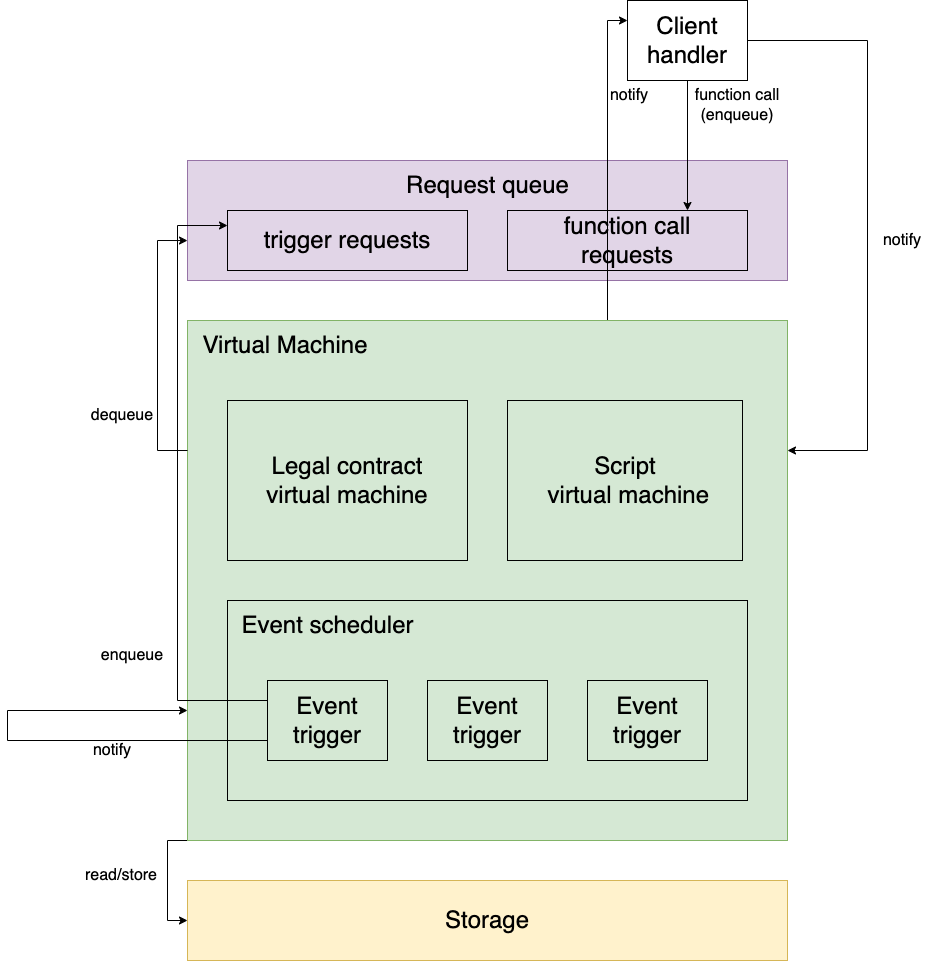
\includegraphics[width=0.9\textwidth]{immagini/capitolo-5/vm.png}
		\caption{Virtual machine.}
		\label{fig:vm}
	\end{center}
\end{figure}

\subsection{Requests queue}

This component implements a \textit{queue} that collects all requests made by clients and events for the 
execution of obligations. In the \textit{Stipula} language, for a contract, if at the same time $t$ a 
request from the client to perform a function and a request to perform an obligation arrive 
simultaneously, the execution of the obligation takes \textbf{precedence} over the execution of the 
function requested by the client. To do this, the \verb|RequestQueue| manages two queues: one queue 
collects client requests (\verb|functionCallRequests|) and one queue collects obligation execution 
requests (\verb|obligationRequests|). The \verb|RequestQueue| object has two main methods:
\begin{enumerate}
   \item \verb|enqueue|: this method allows you to add a request to the queue;
   \item \verb|dequeue|: this method allows you to get a request from one of the two queues. If the 
   \verb|obligationRequests| has items, this method will return an item from this queue. If the 
   \verb|obligationRequests| is empty, then an item from the \verb|functionCallRequests| queue will be 
   returned.
\end{enumerate}

Access to these queues is controlled by a \textit{mutex}, in order to properly handle precedence between 
requests. The approach used in the current implementation of the architecture may be a performance 
limitation. In the next chapter some optimizations have been proposed (see \ref{optimizations}).

\subsection{Legal Contract Virtual Machine}
\label{legal-contract-vm}

This component performs contract functions written in \textit{Stipula bytecode}. The instructions of 
this virtual machine are those listed in the \ref{table:bytecode-instructions} table. The functioning of 
this component is very simple: given as input a function of a contract written in bytecode and the 
arguments of this function, the virtual machine sequentially executes each instruction. If one or more 
errors are thrown during the execution of the function, the virtual machine interrupts the execution and 
returns the errors in a special \textit{error stack}; otherwise, execution proceeds until the \verb|HALT| 
instruction is reached, which corresponds to the end of the function.

In this virtual machine there are several \textit{memory zones}:
\begin{enumerate}
  \item \verb|stack|: this is the memory area used by the virtual machine to manipulate the values by 
  means of the instructions read;
  \item \verb|scopeSpace|: this space is dedicated to the storage of local variables to the function;
  \item \verb|argumentsSpace|: this space is dedicated to storing the arguments of the function;
  \item \verb|globalSpace|: this space is dedicated to storing global variables of the contract instance. 
  This space is valued through the information saved in the \textit{Storage} module;
  \item \verb|singleUseSealsToCreate|: this space is dedicated to the temporary storage of the 
  \textit{single-use-seals} to be created. When a function whose code expects to perform one or more 
  \textit{Pay-to-Party} is executed, the execution is not momentarily interrupted to send the payments. We 
  want to ensure atomicity in the execution of the code of a function. Therefore, when the virtual machine 
  realizes that it needs to make a payment to one or more users, it temporarily stores the 
  single-use-seals it has to create. Once the virtual machine finishes executing the function and the 
  execution has not generated any errors, then we will proceed to perform the different 
  \textit{Pay-to-Party};
  \item \verb|createEventRequests|: similarly to the previous point, when the virtual machine reads the 
  \verb|TRIGGER <obligation_function_name>| instruction, it stores in this dedicated space all the events 
  it will have to create once the execution of the function has finished.
\end{enumerate}

In addition, there are two other important fields:
\begin{enumerate}
  \item \verb|executionPointer|: this field indicates the current instruction that has been executed;
  \item \verb|offset|: a full contract is never input to the virtual machine. Only the code of the 
  function to be executed is loaded, therefore the initial value of the \verb|executionPointer| will 
  always be zero. However, when debugging a contract it is useful to have a reference to the line of 
  code that threw an error against the full code of the contract, and not the local code of the function. 
  For this reason, this field stores the line number where the function code starts in the contract and 
  when an error is thrown, in the logs it is possible to have both the line number local to the function 
  and the global line number of the complete contract . Thus, the line number that takes into account the 
  position it is in the contract is given by $\verb|offset| + \verb|executionPointer|$.
\end{enumerate}

\subsection{Script Virtual Machine}
\label{script-vm}

\subsubsection{Single-use-seal and Ownership}
\label{single-use-seals-and-ownerships}

In the previous chapter, the concept of \textit{single-use-seal} (see \ref{single-use-seal-definition}) 
was introduced as a model for asset management. The structure of a single-use-seal was introduced earlier 
(see \ref{pay-to-contract}). To ensure that a single-use-seal can only be spent by the rightful owner, 
this seal is \textit{blocked} using a specific program written in \textit{Script} language. This program 
is saved in the \verb|lockScript| field and is stored along with the other single-use-seal information. 
If a user wants to spend a specific single-use-seal, he must provide proof to prove rightful ownership of 
the funds. The proof is coded as another program written in \textit{Script}, which allows you to 
\textit{unlock} the \verb|unlockScript| program. When a user provides this program as proof of ownership 
of the single-use-seal, he is demonstrating the \textit{ownership} of the funds. In fact, when a user 
wants to make a \textit{Pay-to-Contract}, the user provides the proof in the \verb|FunctionCall| message 
(see section \ref{ownership}). The proof is coded in the Java object \verb|Ownership| and is structured 
as follows:
\begin{enumerate}
  \item \verb|String contractInstanceId|: it indicates to which instance of the contract the payment must 
  be made;
  \item \verb|SingleUseSeal singleUseSeal|: indicate the funds to be spent;
  \item \verb|String unlockScript|: the program that allows you to unlock the \verb|lockScript| contained 
  in the \verb|singleUseSeal| object.
\end{enumerate}

Joining \verb|unlockScript| and \verb|lockScript| it is possible to check if the user is the actual owner 
of the single-use-seal he wants to spend. The main idea of this mechanism was formulated in Bitcoin in 
2009 and is called \textbf{Pay-to-Public-Key-Hash} (\textbf{P2PKH}) \autocite{book:mastering-bitcoin}. 
This was one of the very first mechanisms to be able to make payments in the Bitcoin network. The 
\verb|lockScript| program can only be unlocked if in the \verb|unlockScript| program cryptographic proof 
is provided via the funds holder's private key. In this way, when a user wants to pay for an instance of 
a contract, it is the user himself who voluntarily transfers the \textit{ownership} of a single-use-seal 
to the instance of the contract.

\subsubsection{Script}

In the previous chapter, the \textit{Script} language was introduced (see \ref{script-language}). The 
instructions of this language are very limited and most of them are separate from the instructions of the 
\textit{Legal Contract Virtual Machine}. The instructions of the \textit{Script Virtual Machine} are 
listed in the \ref{table:instructions-svm} table and it is possible to notice the difference in the sets 
of instructions between the two virtual machines in the image \ref{fig:instructions-vms} . Furthermore, 
this language only allows you to handle values that are of type \verb|bool| or \verb|str| (see image 
\ref{fig:types-vms}).

\begin{ThreePartTable}
	\setTableNoteFont{\footnotesize}
  \begin{longtable}{|c|c|}
    \caption{Table of \textit{Script Virtual Machine} instructions.}
    \label{table:instructions-svm}\\
    \noalign{\global\arrayrulewidth0.7pt}
    \hline
    \textbf{Instruction} & \textbf{Behavior} \\ [5pt]
    
    \noalign{\global\arrayrulewidth0.7pt}
    \hline
    
    \verb|PUSH|     & $- \rightarrow *$ \\
    \hline
    
    \verb|HALT|     & $- \rightarrow -$ \\
    \hline
    
    \verb|DUP|      & $* \rightarrow (*, *)$ \\
    \hline

    \verb|SHA256|   & $\verb|str| \rightarrow \verb|str|$ \\
    \hline

    \verb|EQUAL|    & $(\verb|str|, \verb|str|) \rightarrow - || \verb|str|$ \\
    \hline
    
    \verb|CHECKSIG| & $(\verb|str|, \verb|str|) \rightarrow \verb|bool|$ \\
    
    \noalign{\global\arrayrulewidth0.7pt}
    \hline
  \end{longtable}
\end{ThreePartTable}

\begin{figure}[htbp]
	\begin{center}
		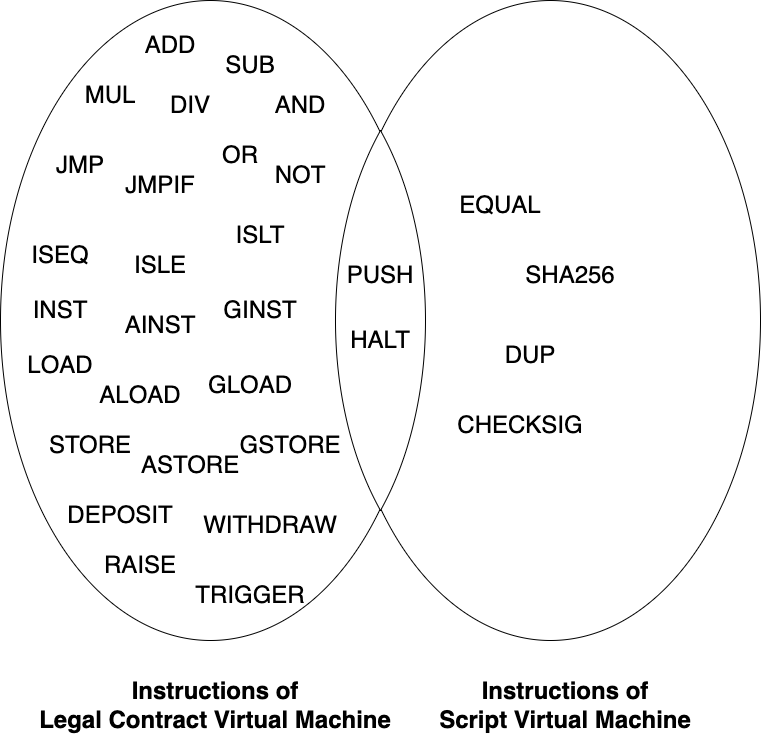
\includegraphics[height=8cm]{immagini/capitolo-5/instructions-vms.png}
		\caption{The instruction sets of the two virtual machines.}
		\label{fig:instructions-vms}
	\end{center}
\end{figure}

\begin{figure}[htbp]
	\begin{center}
		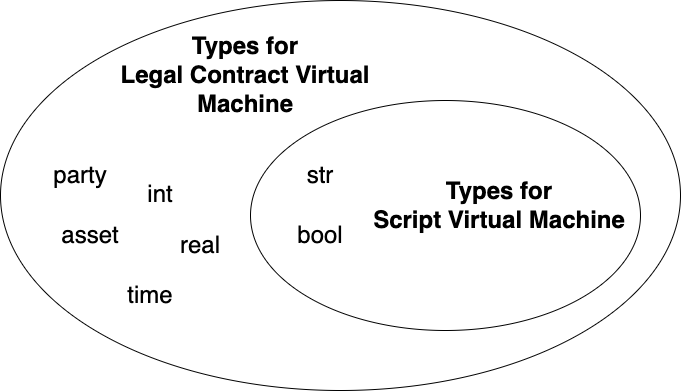
\includegraphics[width=0.8\textwidth]{immagini/capitolo-5/types-vms.png}
		\caption{Sets of the types of the two virtual machines.}
		\label{fig:types-vms}
	\end{center}
\end{figure}

\paragraph{PUSH and HALT}

These statements have the same behavior as those defined for the \textit{Legal Contract Virtual Machine}. 
The only difference is that these statements operate only on values of type \verb|bool| and \verb|str|.

\paragraph{DUP}

This statement takes a value of any type as input and outputs two values that have the same type as the 
input value. This \textit{duplicates} the value received as input, that is, it \textit{pops} from the 
stack and performs two \textit{pushes} of the same value.

\paragraph{SHA256}

This instruction takes as input a value of type \verb|str| and outputs a value of the same type. This 
instruction calculates the SHA256 hash of the input value.

\paragraph{EQUAL}

Given two inputs of type \verb|str|, this statement checks whether the two strings are \textit{equal}. If 
the two values are equal, no value is returned, if instead the values are not equal, then a value of type 
\verb|str| in the \textit{error stack} of the virtual machine.

\paragraph{CHECKSIG}

This instruction takes as input two values of type \verb|str| and outputs a value of type \verb|bool|. The 
first value represents a \textit{public key}, while the second represents a \textit{signature}. This 
instruction allows you to check if, using the public key received as input, the signature is valid or not.

\paragraph{Instruction table}

A summary table of the instructions is shown below: the \verb|-| symbol means that the statement takes no 
value as input or returns no value as output, while the \verb|*| means that the instruction accepts a 
value or outputs a value of type \verb|bool| or \verb|str|.

\subsubsection{LockScript and UnlockScript}
\label{lock-script-and-unlock-script}

Having illustrated the \textit{Script} and \textit{P2PKH} language, give the well-defined structure of 
\verb|lockScript| and \verb|unlockScript|: % citare https://github.com/federicozanardo/stipula-node/issues/23
\begin{enumerate}
  \item \verb|lockScript|: \verb|DUP SHA256 PUSH str <pub_key_hash> EQUAL CHECKSIG|;
  \item \verb|unlockScript|: \verb|PUSH str <signature> PUSH str <pub_key>|;
\end{enumerate}

where,
\begin{enumerate}
  \item \verb|<pub_key>|: is the public key of the user in possession of the single-use-seal;
  \item \verb|<pub_key_hash>|: corresponds to the SHA256 hash of the public key;
  \item \verb|<signature>|: corresponds to the signature of the identifier of the single-use-seal to be 
  spent.
\end{enumerate}

The \verb|<signature>| corresponds to the cryptographic proof that only the user can provide to 
demonstrate possession of the single-use-seal. Signing the single-use-seal identifier provides 
\textit{unique} cryptographic proof and cannot be reused to prove ownership of other funds. So, when the 
user sends the signature and his public key to a \textit{Stipula} server or node, anyone can check it. 
Therefore, if the signature were made using information that can be \textit{reused} to prove possession of 
multiple funds, this would lead to a major security problem, as anyone can verify the signature and reuse 
the information used in the signature to misappropriate other funds.

The union of \verb|lockScript| and \verb|unlockScript|, create the following program which will be 
validated by the virtual machine:

\begin{Verbatim}[numbers=left,xleftmargin=1cm,firstnumber=1,breaklines=true,breakanywhere=true,tabsize=2]
  PUSH str <signature> PUSH str <pub_key> DUP SHA256 PUSH str <pub_key_hash> EQUAL CHECKSIG
\end{Verbatim}

\newpage
The program is evaluated as follows (an example is illustrated by observing the evolution of the stack):
\begin{enumerate}
  \item \verb|PUSH str <signature>|: la \verb|<signature>| is loaded onto the stack
  \begin{ThreePartTable}
    \setTableNoteFont{\footnotesize}
    \begin{longtable}{|>{\centering\arraybackslash}p{2.5cm}|}
      %\label{table:instructions-svm}\\
      \noalign{\global\arrayrulewidth0.7pt}
      \hline

      \\
      \hline
      
      \\
      \hline
      
     \\
      \hline
  
      \\
      \hline
  
      \\
      \hline
      
      \verb|<signature>| \\
      
      \noalign{\global\arrayrulewidth0.7pt}
      \hline
    \end{longtable}
  \end{ThreePartTable}

  \item \verb|PUSH str <pub_key>|: the public key is loaded onto the stack
  \begin{ThreePartTable}
    \setTableNoteFont{\footnotesize}
    \begin{longtable}{|>{\centering\arraybackslash}p{2.5cm}|}
      %\label{table:instructions-svm}\\
      \noalign{\global\arrayrulewidth0.7pt}
      \hline
      
      \\
      \hline
      
     \\
      \hline
  
      \\
      \hline
  
      \verb|<pub_key>|   \\
      \hline
      
      \verb|<signature>| \\
      
      \noalign{\global\arrayrulewidth0.7pt}
      \hline
    \end{longtable}
  \end{ThreePartTable}

  \item \verb|DUP|: you duplicate the last element of the stack, which in this case is the public key
  \begin{ThreePartTable}
    \setTableNoteFont{\footnotesize}
    \begin{longtable}{|>{\centering\arraybackslash}p{2.5cm}|}
      %\label{table:instructions-svm}\\
      \noalign{\global\arrayrulewidth0.7pt}
      \hline
      
      \\
      \hline
      
     \\
      \hline
  
      \verb|<pub_key>|   \\
      \hline
  
      \verb|<pub_key>|   \\
      \hline
      
      \verb|<signature>| \\
      
      \noalign{\global\arrayrulewidth0.7pt}
      \hline
    \end{longtable}
  \end{ThreePartTable}

  \item \verb|SHA256|: the hash of the last element of the stack is computed, which in this case is the 
  previously duplicated public key
  \begin{ThreePartTable}
    \setTableNoteFont{\footnotesize}
    \begin{longtable}{|>{\centering\arraybackslash}p{2.5cm}|}
      %\label{table:instructions-svm}\\
      \noalign{\global\arrayrulewidth0.7pt}
      \hline
      
      \\
      \hline
  
      \verb|<pub_key_hash>|   \\
      \hline
  
      \verb|<pub_key>|   \\
      \hline
      
      \verb|<signature>| \\
      
      \noalign{\global\arrayrulewidth0.7pt}
      \hline
    \end{longtable}
  \end{ThreePartTable}

  \item \verb|PUSH str <pub_key_hash>|: the public key hash is loaded onto the stack. This hash is taken 
  from the \verb|unlockScript|
  \begin{ThreePartTable}
    \setTableNoteFont{\footnotesize}
    \begin{longtable}{|>{\centering\arraybackslash}p{2.5cm}|}
      \noalign{\global\arrayrulewidth0.7pt}
      \hline
      
      \\
      \hline
      
      \verb|<pub_key_hash>| \\
      \hline
  
      \verb|<pub_key_hash>| \\
      \hline
  
      \verb|<pub_key>|      \\
      \hline
      
      \verb|<signature>|    \\
      
      \noalign{\global\arrayrulewidth0.7pt}
      \hline
    \end{longtable}
  \end{ThreePartTable}

  \newpage
  \item \verb|EQUAL|: occurs if the computed hash is the hash of the \verb|unlockScript| it is equal or 
  less
  \begin{ThreePartTable}
    \setTableNoteFont{\footnotesize}
    \begin{longtable}{|>{\centering\arraybackslash}p{2.5cm}|}
      \noalign{\global\arrayrulewidth0.7pt}
      \hline
      
      \\
      \hline
      
      \\
      \hline
  
      \\
      \hline
  
      \verb|<pub_key>|      \\
      \hline
      
      \verb|<signature>|    \\
      
      \noalign{\global\arrayrulewidth0.7pt}
      \hline
    \end{longtable}
  \end{ThreePartTable}

  \item \verb|CHECKSIG|: occurs if the \verb|<signature>| is valid with the \verb|<pub_key>| present in 
  the stack. If the check is successful, \verb|true| will be pushed onto the stack, otherwise \verb|false|
  \begin{ThreePartTable}
    \setTableNoteFont{\footnotesize}
    \begin{longtable}{|>{\centering\arraybackslash}p{2.5cm}|}
      \noalign{\global\arrayrulewidth0.7pt}
      \hline
      
      \\
      \hline
      
      \\
      \hline
  
      \\
      \hline
  
      \\
      \hline
      
      \verb|true| \\
      
      \noalign{\global\arrayrulewidth0.7pt}
      \hline
    \end{longtable}
  \end{ThreePartTable}
\end{enumerate}

The example just illustrated described all the operations that are performed by the 
\textit{Script Virtual Machine}.

\subsection{Description of the execution flow of a function of a contract}

\begin{figure}[htbp]
	\begin{center}
		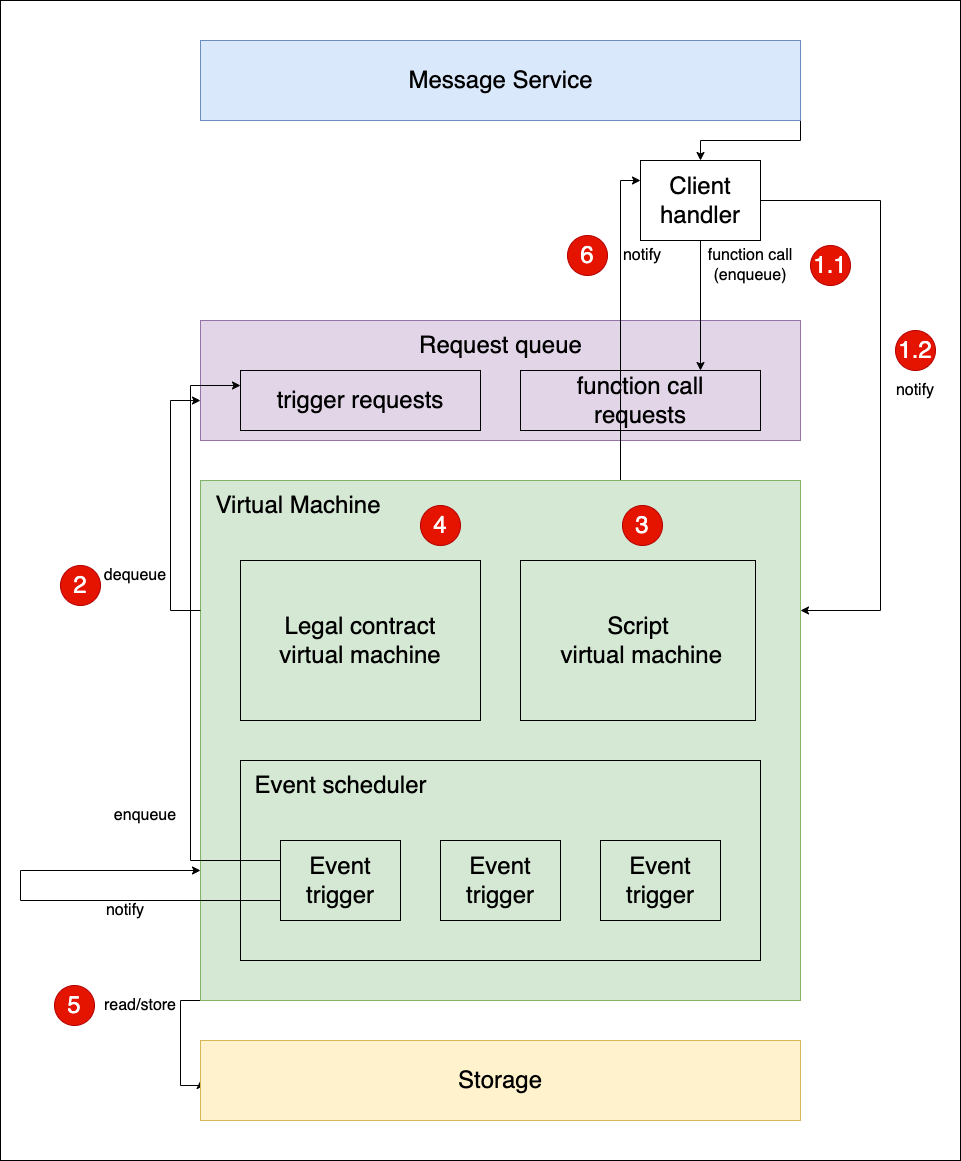
\includegraphics[width=0.9\textwidth]{immagini/capitolo-5/contract-flow.png}
		\caption{Flow of the execution of a function of a function of a contract.}
		\label{fig:contract-flow}
	\end{center}
\end{figure}

This section illustrates the execution flow of a generic contract function (see figure 
\ref{fig:contract-flow}). More precisely, let's suppose that the generic function requires as input a 
value of type \verb|asset|, and that therefore, the user has to make a payment. The flow is as follows:
\begin{enumerate}
  \item A \verb|FunctionCall| message is received (see section \ref{function-call-message}): the 
  \verb|ClientHandler| performs all checks on the format of the message and the signature. After that, the 
  \verb|ClientHandler| adds this new request to the \textit{queue of requests} (\textbf{1.1}, in figure 
  \ref{fig:contract-flow}) and \textit{notifies} the virtual machine (\textbf{1.2}). The notification 
  action of the virtual machine is useful in case the latter is waiting for new requests, but the request 
  queue is empty;
  \item Suppose that the only request in the request queue is the one added in the previous point. The 
  virtual machine dequeues the only request present (\textbf{2});
  \item As mentioned previously, this is a function call that requires an asset as a parameter, therefore, 
  in the \verb|FunctionCall| there is all the information to verify if the funds sent are actually in the 
  user's possession and if they are of the requested quantity. The verification of possession of the sent 
  \textit{single-use-seal} is delegated to the \textit{Script Virtual Machine} (\textbf{3}). If the checks 
  fail, the virtual machine notifies the \verb|ClientHandler| (\textbf{6});
  \item If the verification of the \textit{script} gives a positive result, then we proceed to execute the 
  function indicated by the request. The execution of the function is delegated to the 
  \textit{Legal Contract Virtual Machine} (\textbf{4});
  \item When the execution of the function ends and there are no errors, all the modifications concerning 
  the global variables, the change of the state of the contract and the updating of the single-use-seal, 
  which now can no longer be spent in other contract instances are sent to the \textit{Storage} module 
  (\textbf{5});
  \item Finally, the virtual machine notifies the \verb|ClientHandler|, returning a response regarding the 
  success or failure of the function execution (\textbf{6}).
\end{enumerate}

Next, concrete examples of some contract examples will be shown (see section \ref{examples}). 

\subsection{Pay-to-Party}

Previously, we discussed \textit{Pay-to-Contract}, that is, how a user makes a payment to an instance of 
a contract. When, on the other hand, it is the instance of a contract that has to send payments to one or 
more users, this method is called \textit{Pay-to-Party}. Again, this concept was introduced in the 
previous chapter (see \ref{pay-to-contract-and-pay-to-party}). This mechanism is much simpler than 
\textit{Pay-to-Contract}. When a certain function of a contract expects to send a payment to a user, the 
virtual machine performs all the preliminary checks, for example, it makes sure that it does not disappear 
by the amount of assets from the funds present in the contract instance. Once these checks have been made, 
the virtual machine creates new \textit{single-use-seals}, locking them with the public key of the 
recipient of the funds. Specifically, the \verb|lockScript| will have the following structure: 
\verb|DUP SHA256 PUSH str <pub_key_hash> EQUAL CHECKSIG|, where \verb|<pub_key_hash>| corresponds to the 
SHA256 hash of the payment recipient's public key; By doing so, these funds are now no longer owned by 
the contract instance, but by a specific user. As explained above (see 
\ref{lock-script-and-unlock-script}), only the new owner of the funds will be able to spend them.

\subsection{Obligations}

In the context of the \textit{Stipula} language, \textit{obligations} are formulated into commitments that 
are verified at a given time and issue a corresponding penalty if the obligation has not been fulfilled. 
From an implementation point of view, an obligation consists in the \textit{scheduling} of a 
\textit{event} which at a given moment will call a specific function of the contract. If the obligation 
has been fulfilled, then there won't be the conditions to be able to execute the function, otherwise the 
virtual machine will execute the function, applying penalties.

\subsubsection{Scheduling of an event and description of the flow of execution of an obligation}
\label{execution-flow-for-obligation}

Scheduling always occurs through the execution, by a function, of a piece of code similar to the 
following:

\begin{Verbatim}[numbers=left,xleftmargin=1cm,firstnumber=1,tabsize=2]
  ...
  GLOAD waitTime
  PUSH time now
  ADD
  TRIGGER obligation_1
  ...
\end{Verbatim}

where, from line 2 to line 4 we define the time $t$ in which the obligation must be performed (if the 
conditions allow it), and in line 5 we specify which function must be performed at time $t $. When the 
machine finishes executing the function, a \verb|CreateEventRequest| object is created, in which the name 
of the function to be called and the time $t$ in which this function must be called must be present. After 
that, this object is incorporated into the \verb|EventSchedulingRequest| object, which also contains 
information about the contract instance. This last object is added to a list of \verb|EventTrigger|, 
managed by \verb|EventScheduler|, which collects all the scheduled events. \verb|EventTrigger| is an 
object that extends the \verb|TimerTask| class, which allows you to create a thread and carry out tasks 
at a set time $t$. From here we illustrate the execution flow (see figure \ref{fig:obligation-flow}):
\begin{enumerate}
  \item When the time $t$ is reached, the \verb|EventTrigger| adds the \verb|EventSchedulingRequest| 
  object to the request queue (\textbf{1.1}). This way, the next request that the virtual machine 
  executes will be a request to perform an obligation. After that, \verb|EventTrigger| notifies the 
  virtual machine if it is waiting for new requests, but the request queue is empty (\textbf{1.2});
  \item Suppose that the only request in the request queue is the one added in the previous point. The 
  virtual machine dequeues the only request present (\textbf{2});
  \item If the conditions are satisfied, the virtual machine proceeds to execute the function that 
  represents the obligation, and therefore, to apply the penalties; otherwise the virtual machine does 
  not perform the function. The condition for being able to perform an obligation is if the current state 
  of the contract instance coincides with the state in which the obligation must be performed (\textbf{3});
  \item When the execution of the function ends and there are no errors, all the modifications concerning 
  the global variables, the change of the state of the contract and the updating of the single-use-seal, 
  which now can no longer be spent in other contract instances are sent to the \textit{Storage} module 
  (\textbf{4});
\end{enumerate}

Next, concrete examples of some contract examples will be shown (see section \ref{examples}).

\begin{figure}[htbp]
	\begin{center}
		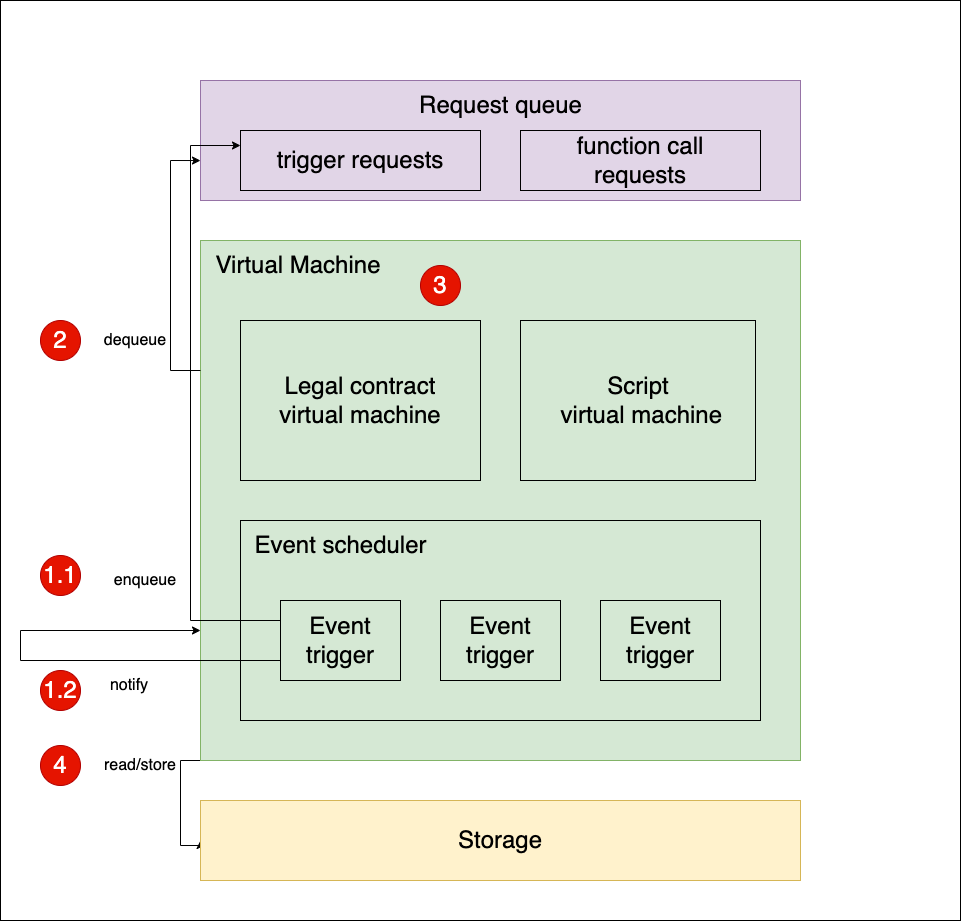
\includegraphics[width=0.9\textwidth]{immagini/capitolo-5/obligation-flow.png}
		\caption{Flow of execution of an obligation.}
		\label{fig:obligation-flow}
	\end{center}
\end{figure}

\section{Storage}
\label{storage}

This module allows you to store all the information regarding contracts, contract instances and their 
evolution, assets and all asset transfers between users and contract instances.

\subsection{LevelDB}

\textit{LevelDB} \autocite{site:leveldb} is an open source \textit{key-value storage library} developed by 
Google. It is a light, fast and efficient storage system capable of handling large amounts of data. 
LevelDB is designed to provide an ordered key-value store with high performance for read and write 
operations. Keys and values can be of any length, and the data is sorted by key in a natural order. The 
data is stored as a \textit{binary blob} and the key can be any stream of bytes. However, it is important 
to note that LevelDB is an unstructured database, which means it doesn't enforce a particular schema or 
data model, and it is up to the application developer to define how to organize and access the data. For 
simplicity in the development of the architecture, it was decided to archive the Java objects directly, 
without designing a particular structure, if not following the key-value structure offered by the library.

LevelDB supports various operations, including basic \textit{CRUD} operations (\textit{create}, 
\textit{read}, \textit{update}, \textit{delete}), \textit{batch} operations, and \ textit{snapshot}.

LevelDB is a library written in C++, but it also has \textit{bindings} for other languages, such as Java, 
Python and Go. This library is used in various applications, including the Bitcoin and Ethereum 
blockchains.

\subsection{Structure}

The \textit{Storage} module consists mainly of four components (see figure \ref{fig:storage-structure}):
\begin{enumerate}
  \item \textit{Asset storage}: all the data concerning the definition of the assets are stored in this 
  component;
  \item \textit{Ownerships storage}: this component stores all spent and unspent \textit{single-use-seals};
  \item \textit{Contracts storage}: this component has the task of storing all the information concerning 
  the contract, such as the source code, the bytecode and the information for instantiating a state 
  machine;
  \item \textit{Contract instances storage}: this component stores all the information that allows you to 
  track the evolution of the state of a contract instance.
\end{enumerate}

\begin{figure}[htbp]
	\begin{center}
		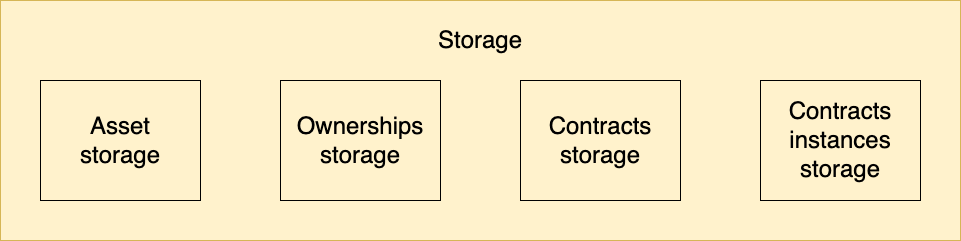
\includegraphics[width=0.9\textwidth]{immagini/capitolo-5/storage.png}
		\caption{Structure of the \textit{Storage} module.}
		\label{fig:storage-structure}
	\end{center}
\end{figure}

\paragraph{Storage serializer}

There are two operations that unite all the components that allow information to be stored and they are:
\begin{enumerate}
  \item \verb|byte[] serialize(T data)|: this method allows you to serialize the data received as input, 
  that is, transforming the input data into a stream of output bytes;
  \item \verb|T deserialize(byte[] bytes)|: this method allows you to deserialize the byte stream 
  received as input into a target object \verb|T|.
\end{enumerate}

Each component of this module extends this class.

\paragraph{Asset storage}

In this class there is a main method, \verb|getAsset|, which allows to obtain all the information 
concerning a specific asset, given an asset identifier as input. There is another method, \verb|seed|, 
which allows you to initialize a certain number of assets when starting the \textit{Stipula} instance. 
This is a method that will be removed in the future: the need for this method to exist is closely related 
to the current limitations of the architecture. See section \ref{database-seeding}, to see how database 
\textit{seeding} can be done, and section \ref{creation-assets-and-distribution} to see a possible 
solution to this limitation.

\paragraph{Ownerships storage}

Also in this class there is the \verb|seed| method, which allows you to create, in a hard-coded way, 
\textit{single-use-seals} for some users. The reason is the same as the one expressed previously, that is, 
the need for this method is due to the current limitations of the implemented architecture.

The other methods in this class are:
\begin{enumerate}
  \item \verb|getFunds|: this method allows you to get all the funds, given a specific input address;
  \item \verb|getFund|: this method allows you to obtain the information of a specific \textit{ownership}, 
  given the property identifier and an address;
  \item \verb|addFunds|: with this method it is possible to add \textit{ownership} to different addresses;
  \item \verb|makeOwnershipSpent|: this method allows you to update a specific \textit{ownership} as 
  \textit{spent}. This method requires as input:
  \begin{enumerate}
    \item The \textit{address} to which the \textit{ownership} is associated;
    \item The identifier of the \textit{ownership} to update;
    \item The identifier of the instance of the contract: this information is important as it is useful to 
    trace from which instance of the contract the payment was made;
    \item \verb|unlockScript|: once the virtual machine has validated the \textit{script} which allows to 
    certify the user's possession of the \textit{ownership}, the missing part of the script is saved, 
    i.e. \verb|unlockScript|. By doing so, this \textit{ownership} can now no longer be spent.
  \end{enumerate}
\end{enumerate}

\paragraph{Contracts storage}

This class contains the following methods:
\begin{enumerate}
  \item \verb|getContract|: this method allows you to obtain information about a specific contract, given 
  the identifier of an input contract;
  \item \verb|saveContract|: this method allows you to store a new contract. If this method is called, 
  the contract has been compiled successfully.
\end{enumerate}

Once a contract is stored in this form, it can no longer be deleted or modified.

\paragraph{Contract instances storage}

This class contains the following methods:
\begin{enumerate}
  \item \verb|getContractInstance|: this method allows to obtain the information of a specific instance of 
  a contract, given the identifier of an instance of an input contract;
  \item \verb|saveContractInstance|: this method allows you to create a new instance of a contract. If 
  this method is called, it means that the \textit{agreement} phase has been successful;
  \item \verb|storeGlobalSpace|: this method allows you to update the \textit{global variables} of a 
  specific instance of a contract. If this method is called, it means that the function execution was 
  successful;
  \item \verb|storeStateMachine|: this method allows you to update the \textit{current state} of the state 
  machine of a contract instance. If this method is called, it means that the function execution was 
  successful.
\end{enumerate}

\section{Examples}
\label{examples}

In this section, concrete examples of code will be introduced to illustrate how the implemented 
implementation works. Examples will include writing the contract in \textit{Stipula}, loading and 
compiling the contract, and running an instance of the contract.

\subsection{Asset swap}
\label{asset-swap}

In this example, there are two actors, Alice and Bob, who want to trade two assets. For simplicity, the 
price variation that these assets may have over time is not taken into consideration, the exchange rate of 
these two assets is fixed by the parties to the contract when a new instance of the contract is made.

For this example there are two versions: in the first version, when Bob deposits his asset, the swap 
happens immediately; in the second version, when both parties deposit their assets, the swap is delegated 
to a \textit{obligation}, which will be triggered after a certain time indicated by the variable 
\verb|waitTimeBeforeSwapping|.

The complete code is present in the appendix \ref{app:asset-swap-complete-code}.

\subsubsection{Agreement}

This first part of the contract defines the variables for:
\begin{enumerate}
  \item The assets: the identifiers of the assets to be exchanged in this contract are specified (line 2);
  \item The quantities of assets to be traded (line 3);
  \item The initial state of the contract state machine (line 4).
\end{enumerate}

\begin{Verbatim}[numbers=left,xleftmargin=1cm,firstnumber=1,breaklines=true,tabsize=2]
  stipula SwapAsset {
    asset assetA:stipula_assetA_ed8i9wk, assetB:stipula_assetB_pl1n5cc
    field amountAssetA, amountAssetB
    init Inactive
\end{Verbatim}

When two parties decide to exchange two specific assets, they make a \textit{agreement}. In the code of 
this function it is possible to notice that the participants of the contract are defined and the values 
for \verb|amountAssetA| and \verb|amountAssetB|, that is, indicate the amount of assets that will have to 
be exchanged. Once this function has been called it means that both parties to the contract are in 
agreement to trade those particular assets, at an agreed rate.

\begin{Verbatim}[numbers=left,xleftmargin=1cm,firstnumber=6,tabsize=2]
  agreement (Alice, Bob)(amountAssetA, amountAssetB) {
        Alice, Bob: amountAssetA, amountAssetB
    } ==> @Inactive
\end{Verbatim}

\newpage
The following bytecode is associated with this function in \textit{Stipula}:
\begin{Verbatim}[numbers=left,xleftmargin=1cm,firstnumber=1,tabsize=2]
  fn agreement Alice,Bob Inactive real,real
  global:
  GINST party Alice
  GINST party Bob
  GINST asset assetA 2 stipula_assetA_ed8i9wk
  GINST asset assetB 2 stipula_assetB_pl1n5cc
  GINST real amountAssetA 2
  GINST real amountAssetB 2
  args:
  PUSH party :Alice
  GSTORE Alice
  PUSH party :Bob
  GSTORE Bob
  PUSH real :amountAssetA
  GSTORE amountAssetA
  PUSH real :amountAssetB
  GSTORE amountAssetB
  start:
  end:
  HALT
\end{Verbatim}

In line 1 it is possible to note the signature of the function, where the name of the function 
(\verb|agreement|), the participants of the contract (\verb|Alice,Bob|), the state in which the instance 
of the contract will go once the execution of the function will have terminated without errors 
(\verb|Inactive|) and the types of the parameters of the function (\verb|real,real|). In this case, the 
function takes two parameters and both must be of type \verb|real|.

From line 2 to line 8, the global variables of the contract are created, i.e. the participants of the 
contract (lines 3-4), the variables that will contain the assets that will have to be exchanged 
(lines 5-6) and the variables that indicate the amount of assets that will have to be deposited 
(lines 7-8).

From line 9 to line 17, the global variables are valued using the values contained in the function 
parameters. In particular:
\begin{enumerate}
  \item Lines 10-13: information about the parties to the contracts is stored (public key and address);
  \item Lines 14-17: the variables indicating the quantity of assets that must be deposited in the 
  contract by each participant in the contract are set.
\end{enumerate}

From line 18 to line 19 the body of the function is defined, which in this case is empty, and in line 20 
the end of the function is indicated by the function \verb|HALT|.

\subsubsection{Deposit of the first asset}

This portion of code allows Alice to deposit a certain amount of assets, agreed during the 
\textit{agreement} phase. In particular:
\begin{enumerate}
  \item Line 10: this function can only be called by Alice and if the contract is in the \verb|@Inactive| 
  state. Note that this function takes a \verb|asset| as an argument (note \verb|[y]|);
  \item Line 11: a check is made to verify if the quantity received as input is equal to the quantity 
  established in the \textit{agreement} phase;
  \item Line 12: this instruction represents the deposit of a certain quantity of assets within the 
  instance of the contract;
  \item Line 14: at the end of the function, the state of the contract will change from \verb|@Inactive| 
  to \verb|@Swap|.
\end{enumerate}

\begin{Verbatim}[numbers=left,xleftmargin=1cm,firstnumber=10,tabsize=2]
  @Inactive Alice : depositAssetA()[y]
        (y == amountAssetA) {
            y -o assetA;
            _
    } ==> @Swap
\end{Verbatim}

The following bytecode is associated with this function in \textit{Stipula}:
\begin{Verbatim}[numbers=left,xleftmargin=1cm,firstnumber=21,tabsize=2]
  fn Inactive Alice depositAssetA Swap asset
  args:
  PUSH asset :y
  AINST asset :y
  ASTORE y
  start:
  ALOAD y
  GLOAD amountAssetA
  ISEQ
  JMPIF if_branch
  RAISE AMOUNT_NOT_EQUAL
  JMP end
  if_branch:
  ALOAD y
  GLOAD assetA
  DEPOSIT assetA
  end:
  HALT
\end{Verbatim}

On line 21 it is possible to note the signature of the function, where the following are specified:
\begin{enumerate}
  \item The state the contract instance must be in in order to call this function (\verb|@Inactive|);
  \item The party that can call this function (\verb|Alice|);
  \item The name of the function (\verb|depositAssetA|);
  \item The state the contract instance will go to once the function's execution has finished without 
  errors (\verb|Swap|);
  \item The type of the function parameter (\verb|asset|).
\end{enumerate}

From line 22 to line 25, the function argument is instantiated. This variable is stored in the argument 
space (\verb|argumentSpace|).

From line 26 to line 37 is the body of the function. In particular, from line 27 to line 30, the virtual 
machine checks if the quantity of assets received as input is equal to that established during the 
\textit{agreement} phase. If the result of this check is \textit{false}, then the virtual machine will 
continue executing first with line 31 and then with line 32, the function execution will terminate. If 
instead the result of the check is \textit{true}, starting from line 30, the virtual machine will execute 
the instructions starting from line 33 in sequence.

From line 34 to line 36, it is possible to note the effective action of \textit{deposit} of assets within 
the instance of the contract (\textit{Pay-to-Contract}). In particular:
\begin{Verbatim}[numbers=left,xleftmargin=1cm,firstnumber=33,tabsize=2]
  ...
  ALOAD y
  GLOAD assetA
  DEPOSIT assetA
  ...
\end{Verbatim}
corresponds to the following line written in \textit{Stipula}
\begin{Verbatim}[numbers=left,xleftmargin=1cm,firstnumber=11,tabsize=2]
  ...
          y -o assetA;
  ...
\end{Verbatim}

\subsubsection{Deposit of the second asset and swap}

The code of this function is very similar to that of the previous function, except for the \textit{swap} 
operation. This function, in fact, allows Bob to deposit the asset in his possession and then to exchange 
the assets between the participants of the contract. In particular, it is possible to observe that line 19 
and line 20 implement the actual asset swap operation, ie: the asset previously deposited by Alice is sent 
to Bob; the asset deposited in this function by Bob is sent to Alice.

\begin{Verbatim}[numbers=left,xleftmargin=1cm,firstnumber=16,tabsize=2]
  @Swap Bob : depositAssetBAndSwap()[y]
        (y == amountAssetB) {
            y -o assetB
            assetB -o Alice
            assetA -o Bob;
            _
    } ==> @End
  }
\end{Verbatim}

The following bytecode is associated with this function in \textit{Stipula}:
\begin{Verbatim}[numbers=left,xleftmargin=1cm,firstnumber=39,tabsize=2]
  fn Swap Bob depositAssetBAndSwap End asset
  args:
  PUSH asset :y
  AINST asset :y
  ASTORE y
  start:
  ALOAD y
  GLOAD amountAssetB
  ISEQ
  JMPIF if_branch
  RAISE AMOUNT_NOT_EQUAL
  JMP end
  if_branch:
  ALOAD y
  GLOAD assetB
  DEPOSIT assetB
  PUSH real 100 2
  GLOAD assetB
  GLOAD Alice
  WITHDRAW assetB
  PUSH real 100 2
  GLOAD assetA
  GLOAD Bob
  WITHDRAW assetA
  end:
  HALT
\end{Verbatim}

Again, the bytecode produced is very similar to that produced for the previous function. It can be seen 
that from line 55 to line 62 the asset swap is implemented. In particular, it is possible to note:
\begin{enumerate}
  \item From line 52 to line 54 there is a \textit{deposit} (\textit{Pay-to-Contract})
  \begin{Verbatim}[numbers=left,xleftmargin=1cm,firstnumber=51,tabsize=2]
    ...
    ALOAD y
    GLOAD assetB
    DEPOSIT assetB
    ...
  \end{Verbatim}
  This piece of code corresponds to the following line written in \textit{Stipula}
  \begin{Verbatim}[numbers=left,xleftmargin=1cm,firstnumber=17,tabsize=2]
    ...
            y -o assetB;
    ...
  \end{Verbatim}
  \item From line 55 to line 58 there is a \textit{withdraw} towards Alice (\textit{Pay-to-Party})
  \begin{Verbatim}[numbers=left,xleftmargin=1cm,firstnumber=54,tabsize=2]
    ...
    PUSH real 100 2
    GLOAD assetB
    GLOAD Alice
    WITHDRAW assetB
    ...
  \end{Verbatim}
  This piece of code corresponds to the following line written in \textit{Stipula}
  \begin{Verbatim}[numbers=left,xleftmargin=1cm,firstnumber=18,tabsize=2]
    ...
            assetB -o Alice;
    ...
  \end{Verbatim}
  \item From line 59 to line 62 there is a \textit{withdraw} towards Bob (\textit{Pay-to-Party})
  \begin{Verbatim}[numbers=left,xleftmargin=1cm,firstnumber=58,tabsize=2]
    ...
    PUSH real 100 2
    GLOAD assetA
    GLOAD Bob
    WITHDRAW assetA
    ...
  \end{Verbatim}
  This piece of code corresponds to the following line written in \textit{Stipula}
  \begin{Verbatim}[numbers=left,xleftmargin=1cm,firstnumber=19,tabsize=2]
    ...
            assetA -o Bob;
    ...
  \end{Verbatim}
\end{enumerate}

\subsubsection{Example of execution}

An example of execution of this contract is illustrated.

\paragraph{Deploy contract}

\begin{figure}[htbp]
	\begin{center}
		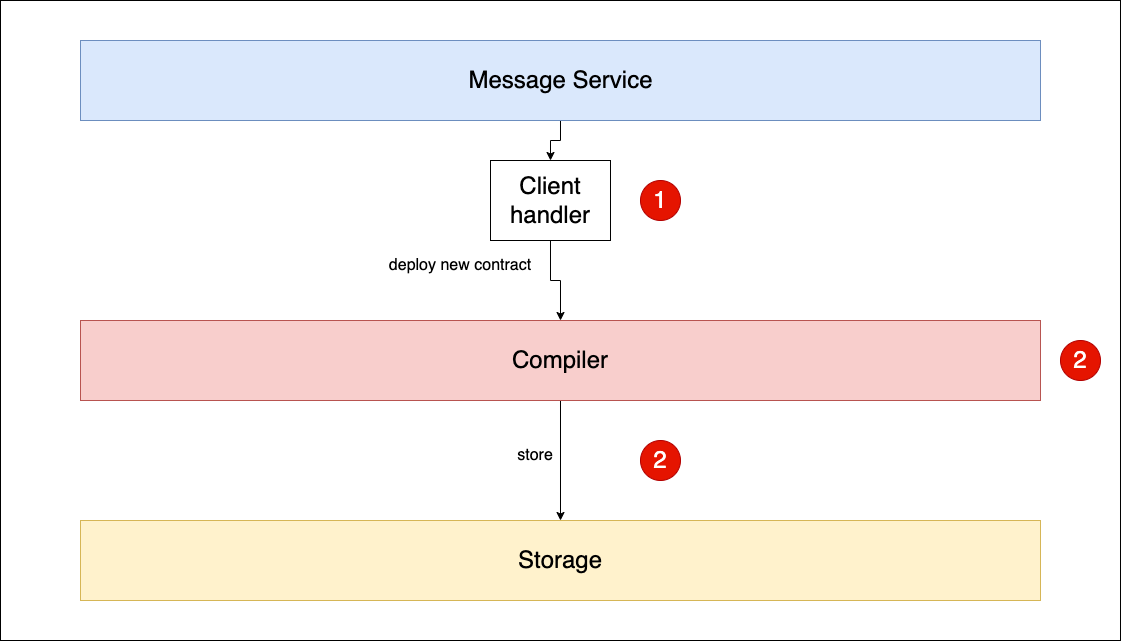
\includegraphics[width=0.9\textwidth]{immagini/capitolo-5/deploy-contract-flow.png}
		\caption{New contract upload execution flow.}
		\label{fig:deploy-contract-flow}
	\end{center}
\end{figure}

The flow for \textit{deploy} a new contract is illustrated in figure \ref{fig:deploy-contract-flow}. The 
request is received by the \verb|MessageService| and via the \verb|ClientHandler| the request is directed 
to the compiler (\textbf{1}). The contract is compiled and if the compilation returns no errors 
(\textbf{2}), it stores the contract and the compiled in the \textit{Storage} module (\textbf{3}).

Request to the server for contract deployment:
{
  \small
  \begin{Verbatim}[numbers=left,xleftmargin=1cm,firstnumber=1,breaklines=true,breakanywhere=true,tabsize=2]
    {
      "message": {
        "sourceCode": "stipula SwapAsset {\n    asset assetA:stipula_assetA_ed8i9wk, assetB:stipula_assetB_pl1n5cc\n    field amountAssetA, amountAssetB\n    init Inactive\n\n    agreement (Alice, Bob)(amountAssetA, amountAssetB) {\n        Alice, Bob: amountAssetA, amountAssetB\n    } ==> @Inactive\n\n    @Inactive Alice : depositAssetA()[y]\n        (y == amountAssetA) {\n            y -o assetA;\n            _\n    } ==> @Swap\n\n    @Swap Bob : depositAssetBAndSwap()[y]\n        (y == amountAssetB) {\n            y -o assetB\n            assetB -o Alice\n            assetA -o Bob;\n            _\n    } ==> @End\n}",
        "type": "DeployContract"
      },
      "signatures": {
        "MIGfMA0GCSqGSIb3DQEBAQUAA4GNADCBiQKBgQCo/GjVKS+3gAA55+kko41yINdOcCLQMSBQyuTTkKHE1mhu/TgOpivM0wLPsSga8hQMr3+v3aR0IF/vfCRf6SdiXmWx/jflmEXtnT6fkGcnV6dGNUpHWXSpwUIDt0N88jfnEqekx4S+KDCKg99sGEeHeT65fKS8lB0gjHMt9AOriwIDAQAB": "V5gJHSax5J5nWYZlyhJr+RdJhbWrog9/urvyfWPTNWf6jkLRT16xAdLYBR1NucOmKTf9iW6mVMVpUxtrGPXktTUEIzxJpp81jR06hDBUpH0Eu6pkiw9nomTUZvuCX9DR/+WOSBz0jMO5lOznl6At3OP1mXsgNyRtPJTi2q4yHs0="
      }
    }
  \end{Verbatim}
}

Server response:
{
  \small
  \begin{Verbatim}[numbers=left,xleftmargin=1cm,firstnumber=1,breaklines=true,breakanywhere=true,tabsize=2]
    {
      "data": "d50ed1a3-7a65-4238-867e-df48536b7243",
      "statusCode": 200,
      "statusMessage": "Success",
      "type": "SuccessDataResponse"
    }
  \end{Verbatim}
}

The value in the \verb|data| field indicates the identifier of the deployed contract.

\paragraph{Single-use-seals by Alice}

{
  \small
  \begin{figure}[htbp]
    \begin{center}
      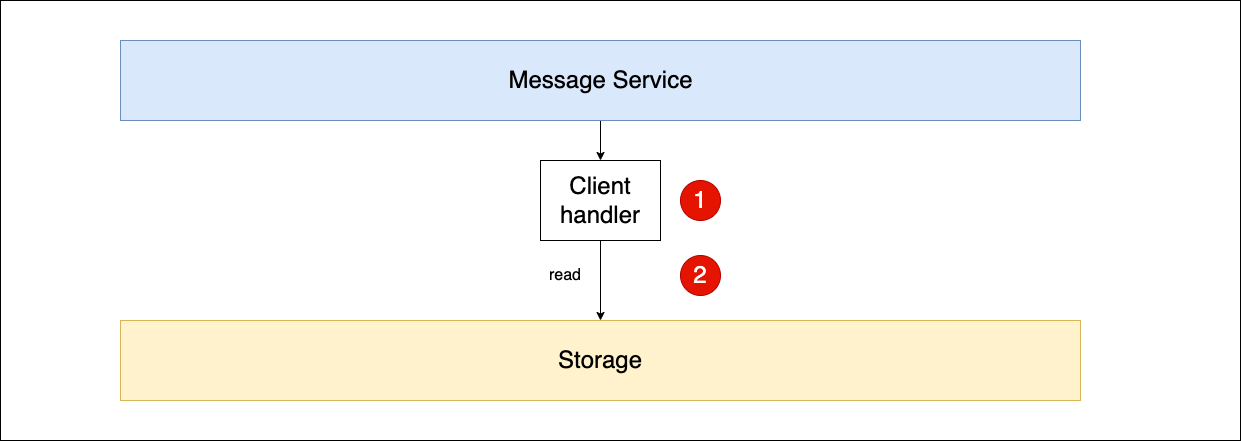
\includegraphics[width=0.9\textwidth]{immagini/capitolo-5/get-funds-flow.png}
      \caption{Execution flow for Alice's funds read request.}
      \label{fig:get-funds-flow}
    \end{center}
  \end{figure}
}

The description of the following flow is illustrated in figure \ref{fig:get-funds-flow}. When a user wants 
to know the available funds associated with his address, the user sends a particular message (\textbf{1}). 
The request is directed to the \textit{Storage} module (\textbf{2}) and the availability of funds is sent 
to the user in response.

Request to the server to get the single-use-seals in Alice's possession:
{
  \small
  \begin{Verbatim}[numbers=left,xleftmargin=1cm,firstnumber=1,breaklines=true,breakanywhere=true,tabsize=2]
    {
      "message": {
        "address": "ubL35Am7TimL5R4oMwm2OxgAYA3XT3BeeDE56oxqdLc=",
        "type": "GetOwnershipsByAddress"
      },
      "signatures": {
        "MIGfMA0GCSqGSIb3DQEBAQUAA4GNADCBiQKBgQCo/GjVKS+3gAA55+kko41yINdOcCLQMSBQyuTTkKHE1mhu/TgOpivM0wLPsSga8hQMr3+v3aR0IF/vfCRf6SdiXmWx/jflmEXtnT6fkGcnV6dGNUpHWXSpwUIDt0N88jfnEqekx4S+KDCKg99sGEeHeT65fKS8lB0gjHMt9AOriwIDAQAB": "MomZTc63z7PfH35c1dL4tjXebcsW+0Zxl0nP1NQdcUFws98DX+bMWI7L0C6IO5lxvkYve4zdio1Crn97FXvngK4aVfiEZEnHOJ0tstq7uQYGErM3DDAABqPq8HH5yoKnLST2LWpO0oD8G/VXvIE6qMT5D34W1Ci0q4uh+7y3EcY="
      }
    }
  \end{Verbatim}
}

Server response:
{
  \small
  \begin{Verbatim}[numbers=left,xleftmargin=1cm,firstnumber=1,breaklines=true,breakanywhere=true,tabsize=2]
    {
      "data": "[
          Ownership{
            id='2b4a4614-3bb4-4554-93fe-c034c3ba5a9c', 
            singleUseSeal=SingleUseSeal{
              assetId='stipula_assetA_ed8i9wk', 
              amount=RealType{
                value=1400, 
                decimals=2
              }, 
              lockScript='DUP\nSHA256\nPUSH str ubL35Am7TimL5R4oMwm2OxgAYA3XT3BeeDE56oxqdLc=\nEQUAL\nCHECKSIG\nHALT\n'
            }, 
            unlockScript='', 
            contractInstanceId=''
          }
        ]",
      "statusCode": 200,
      "statusMessage": "Success",
      "type": "SuccessDataResponse"
    }
  \end{Verbatim}
}

\paragraph{Single-use-seals by Bob}

Server request to get Bob's single-use-seals:
{
  \small
  \begin{Verbatim}[numbers=left,xleftmargin=1cm,firstnumber=1,breaklines=true,breakanywhere=true,tabsize=2]
    {
      "message": {
        "address": "f3hVW1Amltnqe3KvOT00eT7AU23FAUKdgmCluZB+nss=",
        "type": "GetOwnershipsByAddress"
      },
      "signatures": {
        "MIGfMA0GCSqGSIb3DQEBAQUAA4GNADCBiQKBgQDErzzgD2ZslZxciFAiX3/ot7lrkZDw4148jFZrsDZPE6CVs9xXFSHGgy/mFvIFLXhnChO6Nyd2be3lbgeavLMCMVUiTStXr117Km17keWpb3sItkKKsLFBOcIIU8XXowI/OhzQN2XPZYESHgjdQ5vwEj2YyueiS7WKP94YWz/pswIDAQAB": "hSNodnUyusffNlv+KNq4605pFvqh91pVspFhTgbmWccE/LKM6h4bedpvTgMHoVDezvA7v2XTzmLG5eL3lOeA6I2xJMH32DcV60IPSoh61oVHnwPQcQHY039D4y5VSJ0GMQJKIcTEq3fqIdabg7261xUaegHUnXrcyynh9GpMJxk="
      }
    }
  \end{Verbatim}
}

Server response:
{
  \small
  \begin{Verbatim}[numbers=left,xleftmargin=1cm,firstnumber=1,breaklines=true,breakanywhere=true,tabsize=2]
    {
      "data": "[
          Ownership{
            id='7a19f50e-eae9-461d-bd58-9946ea39ccf0', 
            singleUseSeal=SingleUseSeal{
              assetId='stipula_assetB_pl1n5cc', 
              amount=RealType{
                value=1100, 
                decimals=2
              }, 
              lockScript='DUP\nSHA256\nPUSH str f3hVW1Amltnqe3KvOT00eT7AU23FAUKdgmCluZB+nss=\nEQUAL\nCHECKSIG\nHALT\n'
            }, 
            unlockScript='', 
            contractInstanceId=''
          }
        ]",
      "statusCode": 200,
      "statusMessage": "Success",
      "type": "SuccessDataResponse"
    }
  \end{Verbatim}
}

\paragraph{Agreement}

The description of the following flow is illustrated in figure \ref{fig:contract-flow}. When users have 
agreed to execute an agreement, an \verb|AgreementCall| message is sent (see 
\ref{agreement-call-message}). This request is placed in the request queue (\textbf{1.1} and 
\textbf{1.2}). The virtual machine dequeues the request (\textbf{2}) and the function \textit{agreement} 
(\textbf{4}) is executed. Once the execution of the function has finished without errors, the result of 
the processing will be stored in the \textit{Storage} module (\textbf{5}) and finally the virtual machine 
will notify the client of the success of the operation (\textbf{ 6}).

Request to the server to make the \verb|agreement| function call:
{
  \small
  \begin{Verbatim}[numbers=left,xleftmargin=1cm,firstnumber=1,breaklines=true,breakanywhere=true,tabsize=2]
    {
      "message": {
        "contractId": "d50ed1a3-7a65-4238-867e-df48536b7243",
        "arguments": [
          {
            "argument": {
              "first": "real",
              "second": "amountAssetA",
              "third": "1400 2"
            }
          },
          {
            "argument": {
              "first": "real",
              "second": "amountAssetB",
              "third": "1100 2"
            }
          }
        ],
        "parties": {
          "Bob": {
            "address": "f3hVW1Amltnqe3KvOT00eT7AU23FAUKdgmCluZB+nss=",
            "publicKey": "MIGfMA0GCSqGSIb3DQEBAQUAA4GNADCBiQKBgQDErzzgD2ZslZxciFAiX3/ot7lrkZDw4148jFZrsDZPE6CVs9xXFSHGgy/mFvIFLXhnChO6Nyd2be3lbgeavLMCMVUiTStXr117Km17keWpb3sItkKKsLFBOcIIU8XXowI/OhzQN2XPZYESHgjdQ5vwEj2YyueiS7WKP94YWz/pswIDAQAB"
          },
          "Alice": {
            "address": "ubL35Am7TimL5R4oMwm2OxgAYA3XT3BeeDE56oxqdLc=",
            "publicKey": "MIGfMA0GCSqGSIb3DQEBAQUAA4GNADCBiQKBgQCo/GjVKS+3gAA55+kko41yINdOcCLQMSBQyuTTkKHE1mhu/TgOpivM0wLPsSga8hQMr3+v3aR0IF/vfCRf6SdiXmWx/jflmEXtnT6fkGcnV6dGNUpHWXSpwUIDt0N88jfnEqekx4S+KDCKg99sGEeHeT65fKS8lB0gjHMt9AOriwIDAQAB"
          }
        },
        "type": "AgreementCall"
      },
      "signatures": {
        "MIGfMA0GCSqGSIb3DQEBAQUAA4GNADCBiQKBgQDErzzgD2ZslZxciFAiX3/ot7lrkZDw4148jFZrsDZPE6CVs9xXFSHGgy/mFvIFLXhnChO6Nyd2be3lbgeavLMCMVUiTStXr117Km17keWpb3sItkKKsLFBOcIIU8XXowI/OhzQN2XPZYESHgjdQ5vwEj2YyueiS7WKP94YWz/pswIDAQAB": "crMKGFVc5QYmYfbyxDaqhXEi0/GRO+j2OD8HtBbysVm1/+2D+nFATAOvm+LbDtLMMBHxTE8a4JHzMN1DZ1uokkwHKyv80/IVMLwjZi6RFl1Jk7jUpUq6nBCPfqfa7u2IKtzv0joJXR/8BNyN3u6+PReS+4N530+ESN3W2P3tIFk=",
        "MIGfMA0GCSqGSIb3DQEBAQUAA4GNADCBiQKBgQCo/GjVKS+3gAA55+kko41yINdOcCLQMSBQyuTTkKHE1mhu/TgOpivM0wLPsSga8hQMr3+v3aR0IF/vfCRf6SdiXmWx/jflmEXtnT6fkGcnV6dGNUpHWXSpwUIDt0N88jfnEqekx4S+KDCKg99sGEeHeT65fKS8lB0gjHMt9AOriwIDAQAB": "OK9fuuEHTIV5gjtghgvFqsJZI98Ip7IYXvph0J79kTwfRVvJnH5mX9Rs/lDUWnznOmY3HTADwn4QgzMQgdu+qAfixoyJWvZJZ8XjNo/N1YI3nnaaXhvkpR80SHhxqhFLfET6rAx5qXpziOZS7NfcIasn6Lj35hbQCfcjKvxf76w="
      }
    }
  \end{Verbatim}
}

Server response:
{
  \small
  \begin{Verbatim}[numbers=left,xleftmargin=1cm,firstnumber=1,breaklines=true,breakanywhere=true,tabsize=2]
    {
      "data": "e9cbb96e-4d20-47d2-80e6-5b56701800b1",
      "statusCode": 200,
      "statusMessage": "Success",
      "type": "SuccessDataResponse"
    }
  \end{Verbatim}
}

The value in the \verb|data| field indicates the identifier of the created contract instance.

\paragraph{depositAssetA call}

In this function Alice has to make a \textit{Pay-to-Contract}. Compared to the description of the previous 
flow, before the \textit{Legal Contract Virtual Machine} executes the function, it is necessary to check 
that the \textit{single-use-seal} sent by Alice actually belongs to Alice and is of the quantity requested 
by the instance of the contract. To do this, it is necessary to carry out these checks with the 
\textit{Script Virtual Machine} (see point \textbf{3} of figure \ref{fig:contract-flow}). Once these 
checks have been completed, the virtual machine will be able to proceed with the execution of the 
function requested by Alice.

Request to the server to make the \verb|depositAssetA| function call:
{
  \small
  \begin{Verbatim}[numbers=left,xleftmargin=1cm,firstnumber=1,breaklines=true,breakanywhere=true,tabsize=2]
    {
      "message": {
        "contractInstanceId": "e9cbb96e-4d20-47d2-80e6-5b56701800b1",
        "functionName": "depositAssetA",
        "arguments": [
          {
            "argument": {
              "first": "asset",
              "second": "y",
              "third": {
                "ownershipId": "2b4a4614-3bb4-4554-93fe-c034c3ba5a9c",
                "address": "ubL35Am7TimL5R4oMwm2OxgAYA3XT3BeeDE56oxqdLc=",
                "unlockScript": "PUSH str PLjodnT+m3RNIitQAPBDCsRmJPHCqrwZOY/CPiHFZGnl+DRN6soqxMy3ehTFaUwxBjjf7qfBfvTDq5oBItTFrtz1Rn5SDS1ybdbkwpKaOXVglNOw7ZEG9bbZ1mo1oA7IAjRiIilzUetCstE5rPZIf9XOXr/RQ5AHkZUn2CztsvA=\nPUSH str MIGfMA0GCSqGSIb3DQEBAQUAA4GNADCBiQKBgQCo/GjVKS+3gAA55+kko41yINdOcCLQMSBQyuTTkKHE1mhu/TgOpivM0wLPsSga8hQMr3+v3aR0IF/vfCRf6SdiXmWx/jflmEXtnT6fkGcnV6dGNUpHWXSpwUIDt0N88jfnEqekx4S+KDCKg99sGEeHeT65fKS8lB0gjHMt9AOriwIDAQAB\n"
              }
            }
          }
        ],
        "type": "FunctionCall"
      },
      "signatures": {   
        "MIGfMA0GCSqGSIb3DQEBAQUAA4GNADCBiQKBgQCo/GjVKS+3gAA55+kko41yINdOcCLQMSBQyuTTkKHE1mhu/TgOpivM0wLPsSga8hQMr3+v3aR0IF/vfCRf6SdiXmWx/jflmEXtnT6fkGcnV6dGNUpHWXSpwUIDt0N88jfnEqekx4S+KDCKg99sGEeHeT65fKS8lB0gjHMt9AOriwIDAQAB": "MVm0fv9zBntC7ElPhNYaISpgmOdCh8blRsvkU2gtulbWQvwg/CuKtcOIHxakTrffnrW7iw/KLB0n46HulBL6KAcl02U9HSt0+YwX3imJ50QVWU7kmLoMy5d8uQ+seZzXifsaf7OvE1OpAWXNwh7ICsRZv9U6aV39c13SUqwHjTs="
      }
    }
  \end{Verbatim}
}

Server response:
{
  \small
  \begin{Verbatim}[numbers=left,xleftmargin=1cm,firstnumber=1,breaklines=true,breakanywhere=true,tabsize=2]
    {
      "statusCode": 200,
      "statusMessage": "Success",
      "type": "SuccessDataResponse"
    }
  \end{Verbatim}
}

\paragraph{depositAssetBAndSwap call}

Request to the server to make the \verb|depositAssetBAndSwap| function call:
{
  \small
  \begin{Verbatim}[numbers=left,xleftmargin=1cm,firstnumber=1,breaklines=true,breakanywhere=true,tabsize=2]
    {
      "message": {
        "contractInstanceId": "e9cbb96e-4d20-47d2-80e6-5b56701800b1",
        "functionName": "depositAssetBAndSwap",
        "arguments": [
          {
            "argument": {
              "first": "asset",
              "second": "y",
              "third": {
                "ownershipId": "7a19f50e-eae9-461d-bd58-9946ea39ccf0",
                "address": "f3hVW1Amltnqe3KvOT00eT7AU23FAUKdgmCluZB+nss=",
                "unlockScript": "PUSH str Q0bPh9lThyrg1slz9AGDJDJh1BecN9SlGCeVe3BqLod+zO7q0wvIy8tLognHNBkR8e8zKo6nWGQ8qZ7egjOmm5BQsqZzt8xL3gBbR36vgk9J3G9ObiTR2Dd7hMqsqyJnLT3aZUPXGc6RZoM/iUFGJUXhq2T6DStvYNKuAH+Lfow=\nPUSH str MIGfMA0GCSqGSIb3DQEBAQUAA4GNADCBiQKBgQDErzzgD2ZslZxciFAiX3/ot7lrkZDw4148jFZrsDZPE6CVs9xXFSHGgy/mFvIFLXhnChO6Nyd2be3lbgeavLMCMVUiTStXr117Km17keWpb3sItkKKsLFBOcIIU8XXowI/OhzQN2XPZYESHgjdQ5vwEj2YyueiS7WKP94YWz/pswIDAQAB\n"
              }
            }
          }
        ],
        "type": "FunctionCall"
      },
      "signatures": {
        "MIGfMA0GCSqGSIb3DQEBAQUAA4GNADCBiQKBgQDErzzgD2ZslZxciFAiX3/ot7lrkZDw4148jFZrsDZPE6CVs9xXFSHGgy/mFvIFLXhnChO6Nyd2be3lbgeavLMCMVUiTStXr117Km17keWpb3sItkKKsLFBOcIIU8XXowI/OhzQN2XPZYESHgjdQ5vwEj2YyueiS7WKP94YWz/pswIDAQAB": "kh7JupouiEdeLuilXUdoJqAuPVx28JTg9dySp/ZNJGD5+XW8YhhIgiMJYOhGeN6DJTj/x+TmC96uyS8IwssUt/Hulnh2OAZzkc3FljWj1k/XfL0yye95u+YBxg+t8AddQBi+4uA4yOdzb8YdrONlzGu7t0roirmO8SbOqQR1uX8="
      }
    }
  \end{Verbatim}
}

Server response:
{
  \small
  \begin{Verbatim}[numbers=left,xleftmargin=1cm,firstnumber=1,breaklines=true,breakanywhere=true,tabsize=2]
    {
      "statusCode": 200,
      "statusMessage": "Success",
      "type": "SuccessDataResponse"
    }
  \end{Verbatim}
}

\paragraph{Single-use-seals by Alice}

Server request to get Alice's single-use-seals:
{
  \small
  \begin{Verbatim}[numbers=left,xleftmargin=1cm,firstnumber=1,breaklines=true,breakanywhere=true,tabsize=2]
    {
      "message": {
        "address": "ubL35Am7TimL5R4oMwm2OxgAYA3XT3BeeDE56oxqdLc=",
        "type": "GetOwnershipsByAddress"
      },
      "signatures": {
        "MIGfMA0GCSqGSIb3DQEBAQUAA4GNADCBiQKBgQCo/GjVKS+3gAA55+kko41yINdOcCLQMSBQyuTTkKHE1mhu/TgOpivM0wLPsSga8hQMr3+v3aR0IF/vfCRf6SdiXmWx/jflmEXtnT6fkGcnV6dGNUpHWXSpwUIDt0N88jfnEqekx4S+KDCKg99sGEeHeT65fKS8lB0gjHMt9AOriwIDAQAB": "MomZTc63z7PfH35c1dL4tjXebcsW+0Zxl0nP1NQdcUFws98DX+bMWI7L0C6IO5lxvkYve4zdio1Crn97FXvngK4aVfiEZEnHOJ0tstq7uQYGErM3DDAABqPq8HH5yoKnLST2LWpO0oD8G/VXvIE6qMT5D34W1Ci0q4uh+7y3EcY="
      }
    }
  \end{Verbatim}
}

Server response:
{
  \small
  \begin{Verbatim}[numbers=left,xleftmargin=1cm,firstnumber=1,breaklines=true,breakanywhere=true,tabsize=2]
    {
      "data": "[
          Ownership{
            id='2b4a4614-3bb4-4554-93fe-c034c3ba5a9c', 
            singleUseSeal=SingleUseSeal{
              assetId='stipula_assetA_ed8i9wk', 
              amount=RealType{
                value=1400, 
                decimals=2
              }, 
              lockScript='DUP\nSHA256\nPUSH str ubL35Am7TimL5R4oMwm2OxgAYA3XT3BeeDE56oxqdLc=\nEQUAL\nCHECKSIG\nHALT\n'
            }, 
            unlockScript='PUSH str PLjodnT+m3RNIitQAPBDCsRmJPHCqrwZOY/CPiHFZGnl+DRN6soqxMy3ehTFaUwxBjjf7qfBfvTDq5oBItTFrtz1Rn5SDS1ybdbkwpKaOXVglNOw7ZEG9bbZ1mo1oA7IAjRiIilzUetCstE5rPZIf9XOXr/RQ5AHkZUn2CztsvA=\nPUSH str MIGfMA0GCSqGSIb3DQEBAQUAA4GNADCBiQKBgQCo/GjVKS+3gAA55+kko41yINdOcCLQMSBQyuTTkKHE1mhu/TgOpivM0wLPsSga8hQMr3+v3aR0IF/vfCRf6SdiXmWx/jflmEXtnT6fkGcnV6dGNUpHWXSpwUIDt0N88jfnEqekx4S+KDCKg99sGEeHeT65fKS8lB0gjHMt9AOriwIDAQAB\n', 
            contractInstanceId='e9cbb96e-4d20-47d2-80e6-5b56701800b1'
          }, 
          Ownership{
            id='4cbec85d-f17e-4928-a029-7cf0e646a3f6', 
            singleUseSeal=SingleUseSeal{
              assetId='stipula_assetB_pl1n5cc', 
              amount=RealType{
                value=100, 
                decimals=2
              }, 
              lockScript='DUP\nSHA256\nPUSH str ubL35Am7TimL5R4oMwm2OxgAYA3XT3BeeDE56oxqdLc=\nEQUAL\nCHECKSIG\nHALT\n'
            }, 
            unlockScript='', 
            contractInstanceId=''
          }
        ]",
      "statusCode": 200,
      "statusMessage": "Success",
      "type": "SuccessDataResponse"
    }
  \end{Verbatim}
}

It is possible to see that the first single-use-seal has been spent and that's what was deposited in the 
contract instance. Evidence that the funds have been spent is given by the \verb|unlockScript| field. 
While, the second single-use-seal represents the asset that was in Bob's possession.

\paragraph{Single-use-seals by Bob}

Server request to get Bob's single-use-seals:
{
  \small
  \begin{Verbatim}[numbers=left,xleftmargin=1cm,firstnumber=1,breaklines=true,breakanywhere=true,tabsize=2]
    {
      "message": {
        "address": "f3hVW1Amltnqe3KvOT00eT7AU23FAUKdgmCluZB+nss=",
        "type": "GetOwnershipsByAddress"
      },
      "signatures": {
        "MIGfMA0GCSqGSIb3DQEBAQUAA4GNADCBiQKBgQDErzzgD2ZslZxciFAiX3/ot7lrkZDw4148jFZrsDZPE6CVs9xXFSHGgy/mFvIFLXhnChO6Nyd2be3lbgeavLMCMVUiTStXr117Km17keWpb3sItkKKsLFBOcIIU8XXowI/OhzQN2XPZYESHgjdQ5vwEj2YyueiS7WKP94YWz/pswIDAQAB": "hSNodnUyusffNlv+KNq4605pFvqh91pVspFhTgbmWccE/LKM6h4bedpvTgMHoVDezvA7v2XTzmLG5eL3lOeA6I2xJMH32DcV60IPSoh61oVHnwPQcQHY039D4y5VSJ0GMQJKIcTEq3fqIdabg7261xUaegHUnXrcyynh9GpMJxk="
      }
    }
  \end{Verbatim}
}

Server response:
{
  \small
  \begin{Verbatim}[numbers=left,xleftmargin=1cm,firstnumber=1,breaklines=true,breakanywhere=true,tabsize=2]
    {
      "data": "[
          Ownership{
            id='7a19f50e-eae9-461d-bd58-9946ea39ccf0', 
            singleUseSeal=SingleUseSeal{
              assetId='stipula_assetB_pl1n5cc', 
              amount=RealType{
                value=1100, 
                decimals=2
              }, 
              lockScript='DUP\nSHA256\nPUSH str f3hVW1Amltnqe3KvOT00eT7AU23FAUKdgmCluZB+nss=\nEQUAL\nCHECKSIG\nHALT\n'
            }, 
            unlockScript='PUSH str Q0bPh9lThyrg1slz9AGDJDJh1BecN9SlGCeVe3BqLod+zO7q0wvIy8tLognHNBkR8e8zKo6nWGQ8qZ7egjOmm5BQsqZzt8xL3gBbR36vgk9J3G9ObiTR2Dd7hMqsqyJnLT3aZUPXGc6RZoM/iUFGJUXhq2T6DStvYNKuAH+Lfow=\nPUSH str MIGfMA0GCSqGSIb3DQEBAQUAA4GNADCBiQKBgQDErzzgD2ZslZxciFAiX3/ot7lrkZDw4148jFZrsDZPE6CVs9xXFSHGgy/mFvIFLXhnChO6Nyd2be3lbgeavLMCMVUiTStXr117Km17keWpb3sItkKKsLFBOcIIU8XXowI/OhzQN2XPZYESHgjdQ5vwEj2YyueiS7WKP94YWz/pswIDAQAB\n', 
            contractInstanceId='e9cbb96e-4d20-47d2-80e6-5b56701800b1'
          }, 
          Ownership{
            id='bd1f5959-cd8d-4716-8ece-19e1757c6ac2', 
            singleUseSeal=SingleUseSeal{
              assetId='stipula_assetA_ed8i9wk', 
              amount=RealType{
                value=100, 
                decimals=2
              }, 
              lockScript='DUP\nSHA256\nPUSH str f3hVW1Amltnqe3KvOT00eT7AU23FAUKdgmCluZB+nss=\nEQUAL\nCHECKSIG\nHALT\n'
            }, 
            unlockScript='', 
            contractInstanceId=''
          }
        ]",
      "statusCode": 200,
      "statusMessage": "Success",
      "type": "SuccessDataResponse"
    }
  \end{Verbatim}
}

It is possible to see that the first single-use-seal has been spent and that's what was deposited in the contract 
instance. Evidence that the funds have been spent is given by the \verb|unlockScript| field. While, the 
second single-use-seal represents the asset that was in Alice's possession.

\subsection{Asset swap with scheduled event}

The complete code is present in the appendix \ref{app:asset-swap-event-complete-code}. The 
\textit{Stipula} code compared to the previous version does not change much. The only changes made are:
\begin{enumerate}
  \item Line 3: A new global variable \verb|waitTimeBeforeSwapping| is defined. This variable indicates 
  the time needed to wait before being able to swap assets. It is a value that is agreed between the 
  participants of the \textit{agreement} contract;
  \item Lines 6 and 7: it is specified that a value for \verb|waitTimeBeforeSwapping| must be supplied 
  during the \textit{agreement} phase;
  \item Line 14: the state the contract instance will go to once the function is executed 
  \verb|depositAssetA| will exit without errors, it is no longer \verb|@Swap| but \verb|@Deposit|;
  \item Line 16: if Bob wants to deposit his asset, the contract instance must be in the \verb|@Deposit| 
  and no longer \verb|@Swap|. Also, the function name changes from \verb|depositAssetBAndSwap| to 
  \verb|depositAssetB|;
  \item From line 19 to line 23: the code that encodes the \textit{obligation} that will have to be 
  executed at the time indicated in line 19 is defined, that is, an event will be scheduled that will 
  execute the obligation at the time \verb|now + waitTimeBeforeSwapping|;
  \item Line 24: the state the contract instance will go to once the \verb|depositAssetB| will exit 
  without errors, it is no longer \verb|@End| but \verb|@Swap|;
  \item Line 20: in order to execute the obligation at the defined time, the status of the contract 
  instance must be \verb|@Swap|;
  \item Line 23: the state in which the contract instance will go once the execution of the obligation 
  has finished without errors, will be \verb|@End|.
\end{enumerate}

The bytecode is almost similar to the one produced for the previous example, the substantial change 
occurs for the encoding of the \textit{obligation}. In particular:
\begin{enumerate}
  \item Lines 58 to 60: This piece of code is part of the \verb|depositAssetB| function. These specific 
  lines allow to calculate the \textit{absolute} time, necessary to schedule an \textit{event}, which will 
  carry out a particular function call. To indicate where the function code to be executed by the event 
  begins, the \verb|TRIGGER obligation_1| instruction is used. Once the execution of the function is 
  finished, the event will be scheduled and when the time $t$ arrives, the \verb|EventTrigger| will put 
  the request in the request queue (see \ref{execution-flow-for-obligation});
  \item Line 64 to line 75: lines 66 to 75 correspond exactly to lines 55 to 64 of the previous function. 
  However, this code is now part of a particular function, whose signature is defined on line 64. Indeed, 
  it specifies: this code encodes a \textit{obligation} (\verb|obligation|); in order to perform this 
  obligation, the state of the contract instance must be \verb|@Swap|; the name of the function 
  \verb|obligation_1|; the state in which the contract instance will go once the execution of the 
  obligation has finished without errors, will be \verb|@End|.
\end{enumerate}

\subsubsection{Example of execution}

An example of execution of this contract is illustrated in the appendix 
\ref{app:asset-swap-event-complete-execution}. Only a few steps will be shown in this section.

\paragraph{Agreement}

The \textit{agreement} phase is very similar to the previous example, the only change is to set the value 
to the variable \verb|waitTimeBeforeSwapping|.

Request to the server to make the \verb|agreement| function call:
{
  \small
  \begin{Verbatim}[numbers=left,xleftmargin=1cm,firstnumber=1,breaklines=true,breakanywhere=true,tabsize=2]
    {
      "message": {
        "contractId": "79caadf1-abbe-418a-a9a2-bd132a6f3e9e",
        "arguments": [
          {
            "argument": {
              "first": "real",
              "second": "amountAssetA",
              "third": "1400 2"
            }
          },
          {
            "argument": {
              "first": "real",
              "second": "amountAssetB",
              "third": "1100 2"
            }
          },
          {
            "argument": {
              "first": "time",
              "second": "waitTimeBeforeSwapping",
              "third": "100"
            }
          }
        ],
        "parties": {
          "Bob": {
            "address": "f3hVW1Amltnqe3KvOT00eT7AU23FAUKdgmCluZB+nss=",
            "publicKey": "MIGfMA0GCSqGSIb3DQEBAQUAA4GNADCBiQKBgQDErzzgD2ZslZxciFAiX3/ot7lrkZDw4148jFZrsDZPE6CVs9xXFSHGgy/mFvIFLXhnChO6Nyd2be3lbgeavLMCMVUiTStXr117Km17keWpb3sItkKKsLFBOcIIU8XXowI/OhzQN2XPZYESHgjdQ5vwEj2YyueiS7WKP94YWz/pswIDAQAB"
          },
          "Alice": {
            "address": "ubL35Am7TimL5R4oMwm2OxgAYA3XT3BeeDE56oxqdLc=",
            "publicKey": "MIGfMA0GCSqGSIb3DQEBAQUAA4GNADCBiQKBgQCo/GjVKS+3gAA55+kko41yINdOcCLQMSBQyuTTkKHE1mhu/TgOpivM0wLPsSga8hQMr3+v3aR0IF/vfCRf6SdiXmWx/jflmEXtnT6fkGcnV6dGNUpHWXSpwUIDt0N88jfnEqekx4S+KDCKg99sGEeHeT65fKS8lB0gjHMt9AOriwIDAQAB"
          }
        },
        "type": "AgreementCall"
      },
      "signatures": {
        "MIGfMA0GCSqGSIb3DQEBAQUAA4GNADCBiQKBgQDErzzgD2ZslZxciFAiX3/ot7lrkZDw4148jFZrsDZPE6CVs9xXFSHGgy/mFvIFLXhnChO6Nyd2be3lbgeavLMCMVUiTStXr117Km17keWpb3sItkKKsLFBOcIIU8XXowI/OhzQN2XPZYESHgjdQ5vwEj2YyueiS7WKP94YWz/pswIDAQAB": "Wrqyz5udZAGarLbSlxhYD+Ur6+EqTCFiwqBHEL2IsO5Y23Yxv14O3UzknrwK41L5LPUgVxR3K75AAZ4n+UcUdDNHlm9KHN7rqpsbe7v3yK2q8Qkk6c4IYNPDRFy3Zw62HH94O7tx8CzcvRfdX4fi+RItf4Fa7hb8Ui/crxDEQN8=",
        "MIGfMA0GCSqGSIb3DQEBAQUAA4GNADCBiQKBgQCo/GjVKS+3gAA55+kko41yINdOcCLQMSBQyuTTkKHE1mhu/TgOpivM0wLPsSga8hQMr3+v3aR0IF/vfCRf6SdiXmWx/jflmEXtnT6fkGcnV6dGNUpHWXSpwUIDt0N88jfnEqekx4S+KDCKg99sGEeHeT65fKS8lB0gjHMt9AOriwIDAQAB": "o/bdsudfHdR4BBd9EVaGYikksIezSEdwhHELH/f7xRD9g4uokO5g8wHph6LOht5dt9Y+dYt+Qrt+zNZzGUP8a50R7WB2gNz0Jn3zndKnVoBVhsda/zEwIA2pqccP2Sda7zCYiFTfgnmlUZZZfxjtLazBUzDE/vVVFcwtXAHYMXk="
      }
    }
  \end{Verbatim}
}

For simplicity, the value for \verb|waitTimeBeforeSwapping| is equal to 100, that is, after Bob deposits 
his asset, they will wait 100 seconds before exchanging assets.

Server response:
{
  \small
  \begin{Verbatim}[numbers=left,xleftmargin=1cm,firstnumber=1,breaklines=true,breakanywhere=true,tabsize=2]
    {
      "data": "48819afd-e28f-4037-82fd-1d073ee1d318",
      "statusCode": 200,
      "statusMessage": "Success",
      "type": "SuccessDataResponse"
    }
  \end{Verbatim}
}

The value in the \verb|data| field indicates the identifier of the created contract instance.

\paragraph{Event trigger and execution of the obligation}

The call of \verb|depositAssetA| and \verb|depositAssetB| are the same as the previous example. 

From the server logs it can be seen that the event was triggered, the code encoding the obligation was 
loaded and executed:
{
  \small
  \begin{Verbatim}[numbers=left,xleftmargin=1cm,firstnumber=1,breaklines=true,breakanywhere=true,tabsize=2]
    EventTrigger: A new scheduled request has been triggered => EventTriggerSchedulingRequest{
      request=CreateEventRequest{
        obligationFunctionName='obligation_1', 
        time=1680032647
      }, 
      contractId='79caadf1-abbe-418a-a9a2-bd132a6f3e9e', 
      contractInstanceId='48819afd-e28f-4037-82fd-1d073ee1d318'
    }
    EventTrigger: Enqueuing the request...
    EventTrigger: Notifying the virtual machine...
    EventTrigger: Virtual machine notified
    EventTrigger: Removing the request from EventTriggerHandler...
    VirtualMachine: Ready to dequeue a value...
    VirtualMachine: Request received => Pair{
      first=null, 
      second=EventTriggerSchedulingRequest{
        request=CreateEventRequest{
          obligationFunctionName='obligation_1', 
          time=1680032647
        }, 
        contractId='79caadf1-abbe-418a-a9a2-bd132a6f3e9e', 
        contractInstanceId='48819afd-e28f-4037-82fd-1d073ee1d318'
      }
    }
    VirtualMachine: Just received a trigger request
    loadObligationFunction: Loading the obligation function...
    loadObligationFunction: Obligation function loaded
    VirtualMachine: Function
    start:
    PUSH real 100 2
    GLOAD assetB
    GLOAD Alice
    WITHDRAW assetB
    PUSH real 100 2
    GLOAD assetA
    GLOAD Bob
    WITHDRAW assetA
    end:
    HALT
  
    loadBytecode: Loading the bytecode...
    loadBytecode: Bytecode loaded
  
    VirtualMachine: loadBytecode
    start:
    PUSH real 100 2
    GLOAD assetB
    GLOAD Alice
    WITHDRAW assetB
    PUSH real 100 2
    GLOAD assetA
    GLOAD Bob
    WITHDRAW assetA
    end:
    HALT
  
    LegalContractVirtualMachine: execute => Final state of the execution below
    LegalContractVirtualMachine: execute => The stack is empty
  
    LegalContractVirtualMachine: execute => GlobalSpace
    assetA: 13.00 stipula_assetA_ed8i9wk, changed: true
    amountAssetA: 14.00, changed: false
    assetB: 10.00 stipula_assetB_pl1n5cc, changed: true
    amountAssetB: 11.00, changed: false
    Bob: f3hVW1Amltnqe3KvOT00eT7AU23FAUKdgmCluZB+nss= MIGfMA0GCSqGSIb3DQEBAQUAA4GNADCBiQKBgQDErzzgD2ZslZxciFAiX3/ot7lrkZDw4148jFZrsDZPE6CVs9xXFSHGgy/mFvIFLXhnChO6Nyd2be3lbgeavLMCMVUiTStXr117Km17keWpb3sItkKKsLFBOcIIU8XXowI/OhzQN2XPZYESHgjdQ5vwEj2YyueiS7WKP94YWz/pswIDAQAB, changed: false
    Alice: ubL35Am7TimL5R4oMwm2OxgAYA3XT3BeeDE56oxqdLc= MIGfMA0GCSqGSIb3DQEBAQUAA4GNADCBiQKBgQCo/GjVKS+3gAA55+kko41yINdOcCLQMSBQyuTTkKHE1mhu/TgOpivM0wLPsSga8hQMr3+v3aR0IF/vfCRf6SdiXmWx/jflmEXtnT6fkGcnV6dGNUpHWXSpwUIDt0N88jfnEqekx4S+KDCKg99sGEeHeT65fKS8lB0gjHMt9AOriwIDAQAB, changed: false
    waitTimeBeforeSwapping: 100, changed: false
  
    LegalContractVirtualMachine: execute => The argument space is empty
  
    LegalContractVirtualMachine: execute => The data space is empty
  
    Global state of the execution
    running -> false
    executionPointer -> 10
    executionPointer (with offset) -> 74
    length of the program -> 11
    length of the program (with offset) -> 75
    VirtualMachine: Updating the global store...
    VirtualMachine: Global store updated
    VirtualMachine: Ready to dequeue a value...
    VirtualMachine: I'm waiting...
  \end{Verbatim}
}

The description of the following flow is illustrated in figure \ref{fig:obligation-flow}. When the 
\verb|EventTrigger| added the request to the request queue, the virtual machine will dequeue the request 
(\textbf{2}) and execute the function that encodes the obligation. If the conditions exist to execute the 
obligation, then the virtual machine will execute the function (\textbf{3}) and will send the processing 
result to the \textit{Storage} module (\textbf{4}). If there are no conditions to perform the obligation, 
the virtual machine will not perform the function.

\subsection{Bike rental}
\label{bike-rental-example}

The context of use of this agreement has been described above (see section 
\ref{bike-rental-example-definition}). However, since in the current implementation it is not possible to 
send messages to the contract participants, the illustrated bytecode will refer to the code of the 
contract \textit{Stipula} of the appendix \ref{app:bike-rental-complete-code}. In the same appendix 
there is also the complete contract written in \textit{Stipula bytecode}.

\subsubsection{Agreement}

This first part of the contract defines the variables for:
\begin{enumerate}
  \item The asset that the \verb|Borrower| he will have to deposit in order to then be able to pay the 
  \verb|Lender| (line 2);
  \item In line 3 the following are defined:
  \begin{enumerate}
    \item \verb|cost|: the amount of assets that the \verb|Borrower| will have to deposit;
    \item \verb|rentingTime|: the time available for which the \verb|Borrower| will be able to use the 
    service;
    \item \verb|use_code|: represents the bicycle code. This code must be provided by the \verb|Lender|;
  \end{enumerate}
  \item The initial state of the contract state machine (line 4).
\end{enumerate}

\begin{Verbatim}[numbers=left,xleftmargin=1cm,firstnumber=1,tabsize=2]
  stipula BikeRental {
    asset wallet:stipula_coin_asd345
    field cost, rentingTime, use_code
    init Inactive
\end{Verbatim}

When the \textit{agreement} function call is made, the contract parties have found an agreement regarding 
the cost of the service and the duration of the same.

\begin{Verbatim}[numbers=left,xleftmargin=1cm,firstnumber=6,tabsize=2]
  agreement (Lender, Borrower)(cost, rentingTime){
        Lender, Borrower: cost, rentingTime
    } ==> @Inactive
\end{Verbatim}

The following bytecode is associated with this function in \textit{Stipula}:

\begin{Verbatim}[numbers=left,xleftmargin=1cm,firstnumber=1,tabsize=2]
  fn agreement Lender,Borrower Inactive real,time
  global:
  GINST party Lender
  GINST party Borrower
  GINST asset wallet 2 stipula_coin_asd345
  GINST real cost 2
  GINST time rentingTime
  GINST * use_code
  args:
  PUSH party :Lender
  GSTORE Lender
  PUSH party :Borrower
  GSTORE Borrower
  PUSH real :cost
  GSTORE cost
  PUSH time :rentingTime
  GSTORE rentingTime
  start:
  end:
  HALT
\end{Verbatim}

The structure of the code is very similar to that illustrated for the previous examples. The peculiarity 
that can be noticed is found in line 8. The \verb|*| symbol means that the compiler was unable to 
determine the type of the \verb|use_code| variable. Therefore, the type of the variable will have to be 
defined later at runtime.

\subsubsection{The Lender sends the bicycle code}
\label{dynamic-type}

This piece of code allows the \verb|Lender| to send the code of the bicycle to be used by the 
\verb|Borrower|. In particular, in line 11 it is possible to notice that the code provided by the 
\verb|Lender|, through the parameter \verb|z|, is stored in the global variable \verb|use_code|.

\begin{Verbatim}[numbers=left,xleftmargin=1cm,firstnumber=10,tabsize=2]
  @Inactive Lender : offer(z)[] {
    z -> use_code;
    _
  } ==> @Proposal
\end{Verbatim}

\newpage
The following bytecode is associated with this function in \textit{Stipula}:

\begin{Verbatim}[numbers=left,xleftmargin=1cm,firstnumber=21,tabsize=2]
  fn Inactive Lender offer Proposal *
  args:
  PUSH * :z
  AINST * :z
  ASTORE z
  start:
  ALOAD z
  GSTORE use_code
  end:
  HALT
\end{Verbatim}

In the function signature it is possible to see that an argument of any type (except \verb|asset|) is 
accepted. In fact, it will be the \verb|Lender| function call to value the variable and to define its type.

\subsubsection{The Borrower deposits the funds in the instance of the contract}

The code of this function allows the \verb|Borrower| to deposit funds (lines 15 and 16) and to schedule an 
event that will execute the obligation at time \verb|now + rentingTime| (line 17 to line 20). The code 
that encodes the obligation will send the funds contained in the contract instance to the \verb|Lender|.

\begin{Verbatim}[numbers=left,xleftmargin=1cm,firstnumber=14,tabsize=2]
  @Proposal Borrower : accept()[y]
        (y == cost) {
            y -o wallet;
            now + rentingTime >>
                @Using {
                    wallet -o Lender
                } ==> @End
  } ==> @Using
\end{Verbatim}

The following bytecode is associated with this function in \textit{Stipula}:

\begin{Verbatim}[numbers=left,xleftmargin=1cm,firstnumber=31,tabsize=2]
  fn Proposal Borrower accept Using asset
  args:
  PUSH asset :y
  AINST asset :y
  ASTORE y
  start:
  ALOAD y
  GLOAD cost
  ISEQ
  JMPIF if_branch
  RAISE AMOUNT_NOT_EQUAL
  JMP end
  if_branch:
  ALOAD y
  GLOAD wallet
  DEPOSIT wallet
  GLOAD rentingTime
  PUSH time now
  ADD
  TRIGGER obligation_1
  end:
  HALT
\end{Verbatim}

The code is very similar to the example we did earlier for the evented asset swap. The code that 
implements the obligation is defined as follows:
\begin{Verbatim}[numbers=left,xleftmargin=1cm,firstnumber=61,tabsize=2]
  obligation Using obligation_1 End
  start:
  PUSH real 100 2
  GLOAD wallet
  GLOAD Lender
  WITHDRAW wallet
  end:
  HALT
\end{Verbatim}

\subsubsection{End of the contract}

If the event to execute the obligation has not yet been triggered, the \verb|Borrower| can terminate the 
contract by calling the \verb|end| function. Calling this function sends the funds contained in the 
contract instance to the \verb|Lender|.

\begin{Verbatim}[numbers=left,xleftmargin=1cm,firstnumber=22,tabsize=2]
  @Using Borrower : end()[] {
        wallet -o Lender;
        _
  } ==> @End
\end{Verbatim}

The following bytecode is associated with this function in \textit{Stipula}:

\begin{Verbatim}[numbers=left,xleftmargin=1cm,firstnumber=53,tabsize=2]
  fn Using Borrower end End
  start:
  PUSH real 100 2
  GLOAD wallet
  GLOAD Lender
  WITHDRAW wallet
  end:
  HALT
\end{Verbatim}

The code that implements this function, both of the \textit{Stipula} contract and of the bytecode, is 
almost similar to the code that encodes the obligation, illustrated above.

\subsubsection{Example of execution}

An example of execution of this contract is illustrated in the appendix 
\ref{app:bike-rental-complete-execution}. Only a few steps will be shown in this section. For simplicity, 
the value for \verb|rentingTime| is equal to 100, that is, after the \verb|Borrower| has deposited its 
asset, it will take 100 seconds before the \verb|Borrower| terms of using the service.

Two executions were made for this contract:
\begin{enumerate}
  \item On the first run, the \verb|Borrower| calls the \verb|end| function before the event that executes 
  the obligation code is triggered;
  \item In the second execution, instead, the event that executes the obligation code is triggered first 
  and then the \verb|Borrower| calls the \verb|end| function, which will fail.
\end{enumerate}

Most of the steps of the two executions are the same, the steps that differ according to the execution are 
specifically indicated.

\paragraph{offer call}

Request to the server to make the \verb|offer| function call:
{
  \small
  \begin{Verbatim}[numbers=left,xleftmargin=1cm,firstnumber=1,breaklines=true,breakanywhere=true,tabsize=2]
    {
      "message": {
        "contractInstanceId": "4cc1f3c7-5cb4-4528-b15a-8e5cacf5b18a",
        "functionName": "offer",
        "arguments": [
          {
            "argument": {
              "first": "real",
              "second": "z",
              "third": "100 2"
            }
          }
        ],
        "type": "FunctionCall"
      },
      "signatures": {
        "MIGfMA0GCSqGSIb3DQEBAQUAA4GNADCBiQKBgQCo/GjVKS+3gAA55+kko41yINdOcCLQMSBQyuTTkKHE1mhu/TgOpivM0wLPsSga8hQMr3+v3aR0IF/vfCRf6SdiXmWx/jflmEXtnT6fkGcnV6dGNUpHWXSpwUIDt0N88jfnEqekx4S+KDCKg99sGEeHeT65fKS8lB0gjHMt9AOriwIDAQAB": "bJ0xnIhcDlPMmKYx7h8jjX8Q7PaSdqxRg7xq/zTM0vEKqJVDIN0JcT8Qj7jEX5Pwm2YOq+kSwEAxqlPzwoZoQNhe6FPyz6dbj9/LQ0rg79x4QD5ZrCawpcbbtJ/U5l1RPGvl06EdHeQc4YFlsIW4yywD1XlKtfJc7IJwes/iKrE="
      }
    }
  \end{Verbatim}
}

Through this function call, the global variable \verb|use_code| henceforth it will be of type \verb|real| 
(see section \ref{dynamic-type}).

Server response:
{
  \small
  \begin{Verbatim}[numbers=left,xleftmargin=1cm,firstnumber=1,breaklines=true,breakanywhere=true,tabsize=2]
    {
      "statusCode": 200,
      "statusMessage": "Success",
      "type": "SuccessDataResponse"
    }
  \end{Verbatim}
}

\paragraph{accept call}

Request to the server to make the \verb|accept| function call:
{
  \small
  \begin{Verbatim}[numbers=left,xleftmargin=1cm,firstnumber=1,breaklines=true,breakanywhere=true,tabsize=2]
    {
      "message": {
        "contractInstanceId": "4cc1f3c7-5cb4-4528-b15a-8e5cacf5b18a",
        "functionName": "accept",
        "arguments": [
          {
            "argument": {
              "first": "asset",
              "second": "y",
              "third": {
                "ownershipId": "1ce080e5-8c81-48d1-b732-006fa1cc4e2e",
                "address": "f3hVW1Amltnqe3KvOT00eT7AU23FAUKdgmCluZB+nss=",
                "unlockScript": "PUSH str CJ3CdFnd6QiRoNaxxJN6sEYkmhKsSKi0SP5YXiSGhygZs+EMyE2bPrI+hRL4PSA0vLh0X6PNpDhTaPxx4kc1LEk9su8+6kkDvi3xpLG9bDoPjss+LEPXUjPTcGVB/3jITb8W+GmX1kDYhGHKtSuhvxBjTwwbtok4gRDD1BcMX/o=\nPUSH str MIGfMA0GCSqGSIb3DQEBAQUAA4GNADCBiQKBgQDErzzgD2ZslZxciFAiX3/ot7lrkZDw4148jFZrsDZPE6CVs9xXFSHGgy/mFvIFLXhnChO6Nyd2be3lbgeavLMCMVUiTStXr117Km17keWpb3sItkKKsLFBOcIIU8XXowI/OhzQN2XPZYESHgjdQ5vwEj2YyueiS7WKP94YWz/pswIDAQAB\n"
              }
            }
          }
        ],
        "type": "FunctionCall"
      },
      "signatures": {
        "MIGfMA0GCSqGSIb3DQEBAQUAA4GNADCBiQKBgQDErzzgD2ZslZxciFAiX3/ot7lrkZDw4148jFZrsDZPE6CVs9xXFSHGgy/mFvIFLXhnChO6Nyd2be3lbgeavLMCMVUiTStXr117Km17keWpb3sItkKKsLFBOcIIU8XXowI/OhzQN2XPZYESHgjdQ5vwEj2YyueiS7WKP94YWz/pswIDAQAB": "wL3r61IgwBGau7S7V967ZSA8B0lLiOMi0qai1YGQVFXnCTvL9WDVMGTwp7XXAQ77f23Hw5y6Ho5SFUMRRfaTLguIJBx9twRSUfpTP4bh3K4RB2yg32rkOP16G2vIfEirTT+v2wmp1f10pY+dY/QdMzua7EFdQNmL7PhJnA96CpM="
      }
    }
  \end{Verbatim}
}

Server response:
{
  \small
  \begin{Verbatim}[numbers=left,xleftmargin=1cm,firstnumber=1,breaklines=true,breakanywhere=true,tabsize=2]
    {
      "statusCode": 200,
      "statusMessage": "Success",
      "type": "SuccessDataResponse"
    }
  \end{Verbatim}
}

\paragraph{Version 1 - end call}

Request to the server to make the \verb|end| function call:
{
  \small
  \begin{Verbatim}[numbers=left,xleftmargin=1cm,firstnumber=1,breaklines=true,breakanywhere=true,tabsize=2]
    {
      "message": {
        "contractInstanceId": "4cc1f3c7-5cb4-4528-b15a-8e5cacf5b18a",
        "functionName": "end",
        "arguments": [],
        "type": "FunctionCall"
      },
      "signatures": {
        "MIGfMA0GCSqGSIb3DQEBAQUAA4GNADCBiQKBgQDErzzgD2ZslZxciFAiX3/ot7lrkZDw4148jFZrsDZPE6CVs9xXFSHGgy/mFvIFLXhnChO6Nyd2be3lbgeavLMCMVUiTStXr117Km17keWpb3sItkKKsLFBOcIIU8XXowI/OhzQN2XPZYESHgjdQ5vwEj2YyueiS7WKP94YWz/pswIDAQAB": "hU6i0eGRNcZB+ZCxeLCPBM31iai412yczQ4/Td+roq9jnBU7agWfuOyVl/6fCKdTZcKkxASJs1tCpe4bLlpUHt01lFlGM8n9+sPHXl+1/jXMngmmPhuNUPrtsD7PGeFtuC3JJkcqTq3WkyWz6nVdn55bzX6BxleN/I6MPgmDroc="
      }
    }
  \end{Verbatim}
}

Server response:
{
  \small
  \begin{Verbatim}[numbers=left,xleftmargin=1cm,firstnumber=1,breaklines=true,breakanywhere=true,tabsize=2]
    {
      "statusCode": 200,
      "statusMessage": "Success",
      "type": "SuccessDataResponse"
    }
  \end{Verbatim}
}

\paragraph{Version 1 - Trigger of the event and non-execution of the obligation}

This situation occurs when the customer, who has used the service, has returned the bicycle before the 
end of use of the service.

From the server logs it can be seen that the event was triggered and the code encoding the obligation was 
not executed:
{
  \small
  \begin{Verbatim}[numbers=left,xleftmargin=1cm,firstnumber=1,breaklines=true,breakanywhere=true,tabsize=2]
    EventTrigger: A new scheduled request has been triggered => EventTriggerSchedulingRequest{
      request=CreateEventRequest{
        obligationFunctionName='obligation_1', 
        time=1680036610
      }, 
      contractId='622ad60b-ab1f-4c2c-9f64-1307c046b55d', 
      contractInstanceId='4cc1f3c7-5cb4-4528-b15a-8e5cacf5b18a'
    }
    EventTrigger: Enqueuing the request...
    EventTrigger: Notifying the virtual machine...
    EventTrigger: Virtual machine notified
    EventTrigger: Removing the request from EventTriggerHandler...
    VirtualMachine: Ready to dequeue a value...
    VirtualMachine: Request received => Pair{
      first=null, 
      second=EventTriggerSchedulingRequest{
        request=CreateEventRequest{
          obligationFunctionName='obligation_1', 
          time=1680036610
        }, 
        contractId='622ad60b-ab1f-4c2c-9f64-1307c046b55d', 
        contractInstanceId='4cc1f3c7-5cb4-4528-b15a-8e5cacf5b18a'
      }
    }
    VirtualMachine: Just received a trigger request
    VirtualMachine: This function cannot be called in the current state
    VirtualMachine: Obligation function name => obligation_1
    VirtualMachine: Current state => DfaState{name='End'}
    VirtualMachine: Next state => null
    VirtualMachine: Ready to dequeue a value...
    VirtualMachine: I'm waiting...
  \end{Verbatim}
}

From line 20 to line 22 it can be seen that the obligation has not been performed because the current 
state of the contract instance is \verb|@End|. Instead, the state in which the obligation should be 
executed is \verb|@Using|. For this reason it was not possible to fulfill the obligation.

\paragraph{Version 2 - Event trigger and execution of the obligation}

This situation occurs when the customer, who has used the service, has not returned the bicycle before the 
end of use of the service.

From the server logs it can be seen that the event was triggered, the code encoding the obligation was 
loaded and executed:
{
  \small
  \begin{Verbatim}[numbers=left,xleftmargin=1cm,firstnumber=1,breaklines=true,breakanywhere=true,tabsize=2]
    EventTrigger: A new scheduled request has been triggered => EventTriggerSchedulingRequest{
      request=CreateEventRequest{
        obligationFunctionName='obligation_1', 
        time=1680037664
      }, 
      contractId='51d909ae-45f8-47d2-90de-40699c8a8a3d', 
      contractInstanceId='1a7c6469-b4a3-4c67-8a43-ca60514345f6'
    }
    EventTrigger: Enqueuing the request...
    EventTrigger: Notifying the virtual machine...
    EventTrigger: Virtual machine notified
    EventTrigger: Removing the request from EventTriggerHandler...
    VirtualMachine: Ready to dequeue a value...
    VirtualMachine: Request received => Pair{
      first=null, 
      second=EventTriggerSchedulingRequest{
        request=CreateEventRequest{
          obligationFunctionName='obligation_1', 
          time=1680037664
        }, 
        contractId='51d909ae-45f8-47d2-90de-40699c8a8a3d', 
        contractInstanceId='1a7c6469-b4a3-4c67-8a43-ca60514345f6'
      }
    }
    VirtualMachine: Just received a trigger request
    loadObligationFunction: Loading the obligation function...
    loadObligationFunction: Obligation function loaded
    VirtualMachine: Function
    start:
    PUSH real 100 2
    GLOAD wallet
    GLOAD Lender
    WITHDRAW wallet
    end:
    HALT
  
    loadBytecode: Loading the bytecode...
    loadBytecode: Bytecode loaded
  
    VirtualMachine: loadBytecode
    start:
    PUSH real 100 2
    GLOAD wallet
    GLOAD Lender
    WITHDRAW wallet
    end:
    HALT
  
    LegalContractVirtualMachine: execute => Final state of the execution below
    LegalContractVirtualMachine: execute => The stack is empty
  
    LegalContractVirtualMachine: execute => GlobalSpace
    rentingTime: 100, changed: false
    wallet: 11.00 stipula_coin_asd345, changed: true
    cost: 12.00, changed: false
    Borrower: f3hVW1Amltnqe3KvOT00eT7AU23FAUKdgmCluZB+nss= MIGfMA0GCSqGSIb3DQEBAQUAA4GNADCBiQKBgQDErzzgD2ZslZxciFAiX3/ot7lrkZDw4148jFZrsDZPE6CVs9xXFSHGgy/mFvIFLXhnChO6Nyd2be3lbgeavLMCMVUiTStXr117Km17keWpb3sItkKKsLFBOcIIU8XXowI/OhzQN2XPZYESHgjdQ5vwEj2YyueiS7WKP94YWz/pswIDAQAB, changed: false
    use_code: 1.00, changed: false
    Lender: ubL35Am7TimL5R4oMwm2OxgAYA3XT3BeeDE56oxqdLc= MIGfMA0GCSqGSIb3DQEBAQUAA4GNADCBiQKBgQCo/GjVKS+3gAA55+kko41yINdOcCLQMSBQyuTTkKHE1mhu/TgOpivM0wLPsSga8hQMr3+v3aR0IF/vfCRf6SdiXmWx/jflmEXtnT6fkGcnV6dGNUpHWXSpwUIDt0N88jfnEqekx4S+KDCKg99sGEeHeT65fKS8lB0gjHMt9AOriwIDAQAB, changed: false
  
    LegalContractVirtualMachine: execute => The argument space is empty
  
    LegalContractVirtualMachine: execute => The data space is empty
  
    Global state of the execution
    running -> false
    executionPointer -> 6
    executionPointer (with offset) -> 67
    length of the program -> 7
    length of the program (with offset) -> 68
    VirtualMachine: Updating the global store...
    VirtualMachine: Global store updated
    VirtualMachine: Ready to dequeue a value...
    VirtualMachine: I'm waiting...
  \end{Verbatim}
}

In this case, however, it was possible to execute the code that encodes the obligation because the current 
state of the contract instance is \verb|@Using| and coincides with the state in which the obligation is to 
be performed.

\paragraph{Version 2 - end call}

Here we show the example in which the user tries to call the \verb|end| function, to notify the company 
of the end of using the service. However, the call to this function took place after the maximum time 
established by the contract, and therefore the penalty foreseen by the contract was activated.

Request to the server to make the \verb|end| function call:
{
  \small
  \begin{Verbatim}[numbers=left,xleftmargin=1cm,firstnumber=1,breaklines=true,breakanywhere=true,tabsize=2]
    {
      "message": {
        "contractInstanceId": "1a7c6469-b4a3-4c67-8a43-ca60514345f6",
        "functionName": "end",
        "arguments": [],
        "type": "FunctionCall"
      },
      "signatures": {
        "MIGfMA0GCSqGSIb3DQEBAQUAA4GNADCBiQKBgQDErzzgD2ZslZxciFAiX3/ot7lrkZDw4148jFZrsDZPE6CVs9xXFSHGgy/mFvIFLXhnChO6Nyd2be3lbgeavLMCMVUiTStXr117Km17keWpb3sItkKKsLFBOcIIU8XXowI/OhzQN2XPZYESHgjdQ5vwEj2YyueiS7WKP94YWz/pswIDAQAB": "Ow8gS8d5SChD3E5CgtsnFHTRWskdeWW2IsTLQJk92mS40LfVtPcxuDiIbzL7xWwtUTMFxza+/TSxU+rMsVvMqQLLyUQ4e6UrLO25+Nr7p5x013JGIaxc18G5kqEuS4iEyiqN1479E4ElLROE+VpI5DBAKMegw0h9m5cbtHFN/fA="
      }
    }
  \end{Verbatim}
}

Server response:
{
  \small
  \begin{Verbatim}[numbers=left,xleftmargin=1cm,firstnumber=1,breaklines=true,breakanywhere=true,tabsize=2]
    {
      "data": "This function cannot be called in the current state",
      "statusCode": 404,
      "statusMessage": "Error",
      "type": "ErrorDataResponse"
    }
  \end{Verbatim}
}

\section{Project management}

In this short section we will explain the methods to be able to install an instance of the 
\textit{Stipula} implementation and how the project was managed.

\subsection{Pipeline}
\label{pipelines}

A \textit{pipeline} is a feature offered by a platform that allows for the automation of various tasks in 
the software development process. In essence, it is a script that can be triggered by events, such as a 
new commit in a repository or the opening of a \textit{merge request}. The script can then perform a 
variety of tasks, such as running tests, authoring code, and deploying applications.

Two pipelines were created for this project:
\begin{enumerate}
  \item \verb|run-tests.yml|: it is invoked every time the branch \verb|test| or \verb|master|, or, when a 
  \textit{merge request} is closed. This pipeline allows you to run the tests that have been defined in 
  the project. There is currently only one sample test. The goal is to set up a testing environment for 
  future developments;
  \item \verb|create-and-push-docker-image.yml|: this pipeline is called every time a new \textit{tag} is 
  created. This pipeline allows you to create a \textit{Docker} image and publish it in a dedicated page 
  of the project (see \cite{site:stipula-github-packages-page} and 
  \cite{site:stipula-github-available-packages}).
\end{enumerate}

These pipelines lay the groundwork for creating a more sophisticated test environment and for facilitating 
the installation of an instance of the \textit{Stipula} implementation. In the appendix \ref{app:pipeline} 
there is the code of both pipelines.

\subsection{Issues, milestones ans releases}

To track the evolution of the project and the problems that arise during development, the \textit{issue} 
provided by GitHub was used \autocite{site:stipula-github-issues-section}. To better organize the work, 
these issues have been collected in \textit{milestone} \autocite*{site:stipula-github-milestones-section}. 
The completion of all the issues of a milestone leads to the creation of a \textit{deliverable} 
\autocite{site:stipula-github-releases}, that is, a working version of the project that brings new 
features. Each deliverable is specified by a \textit{release} (note the image \ref{fig:releases}), which 
informs all the features introduced and any problems solved. In the milestones page it is possible to 
notice that the work has been mainly organized in \textit{versions} (note the image 
\ref{fig:milestones-closed}). It can also be noted that the work has been geared towards future versions 
(note the image \ref{fig:milestones-opened}). The current version is \verb|v0.4.2| 
\autocite{site:stipula-github-last-release}. 

\begin{figure}[htbp]
	\begin{center}
		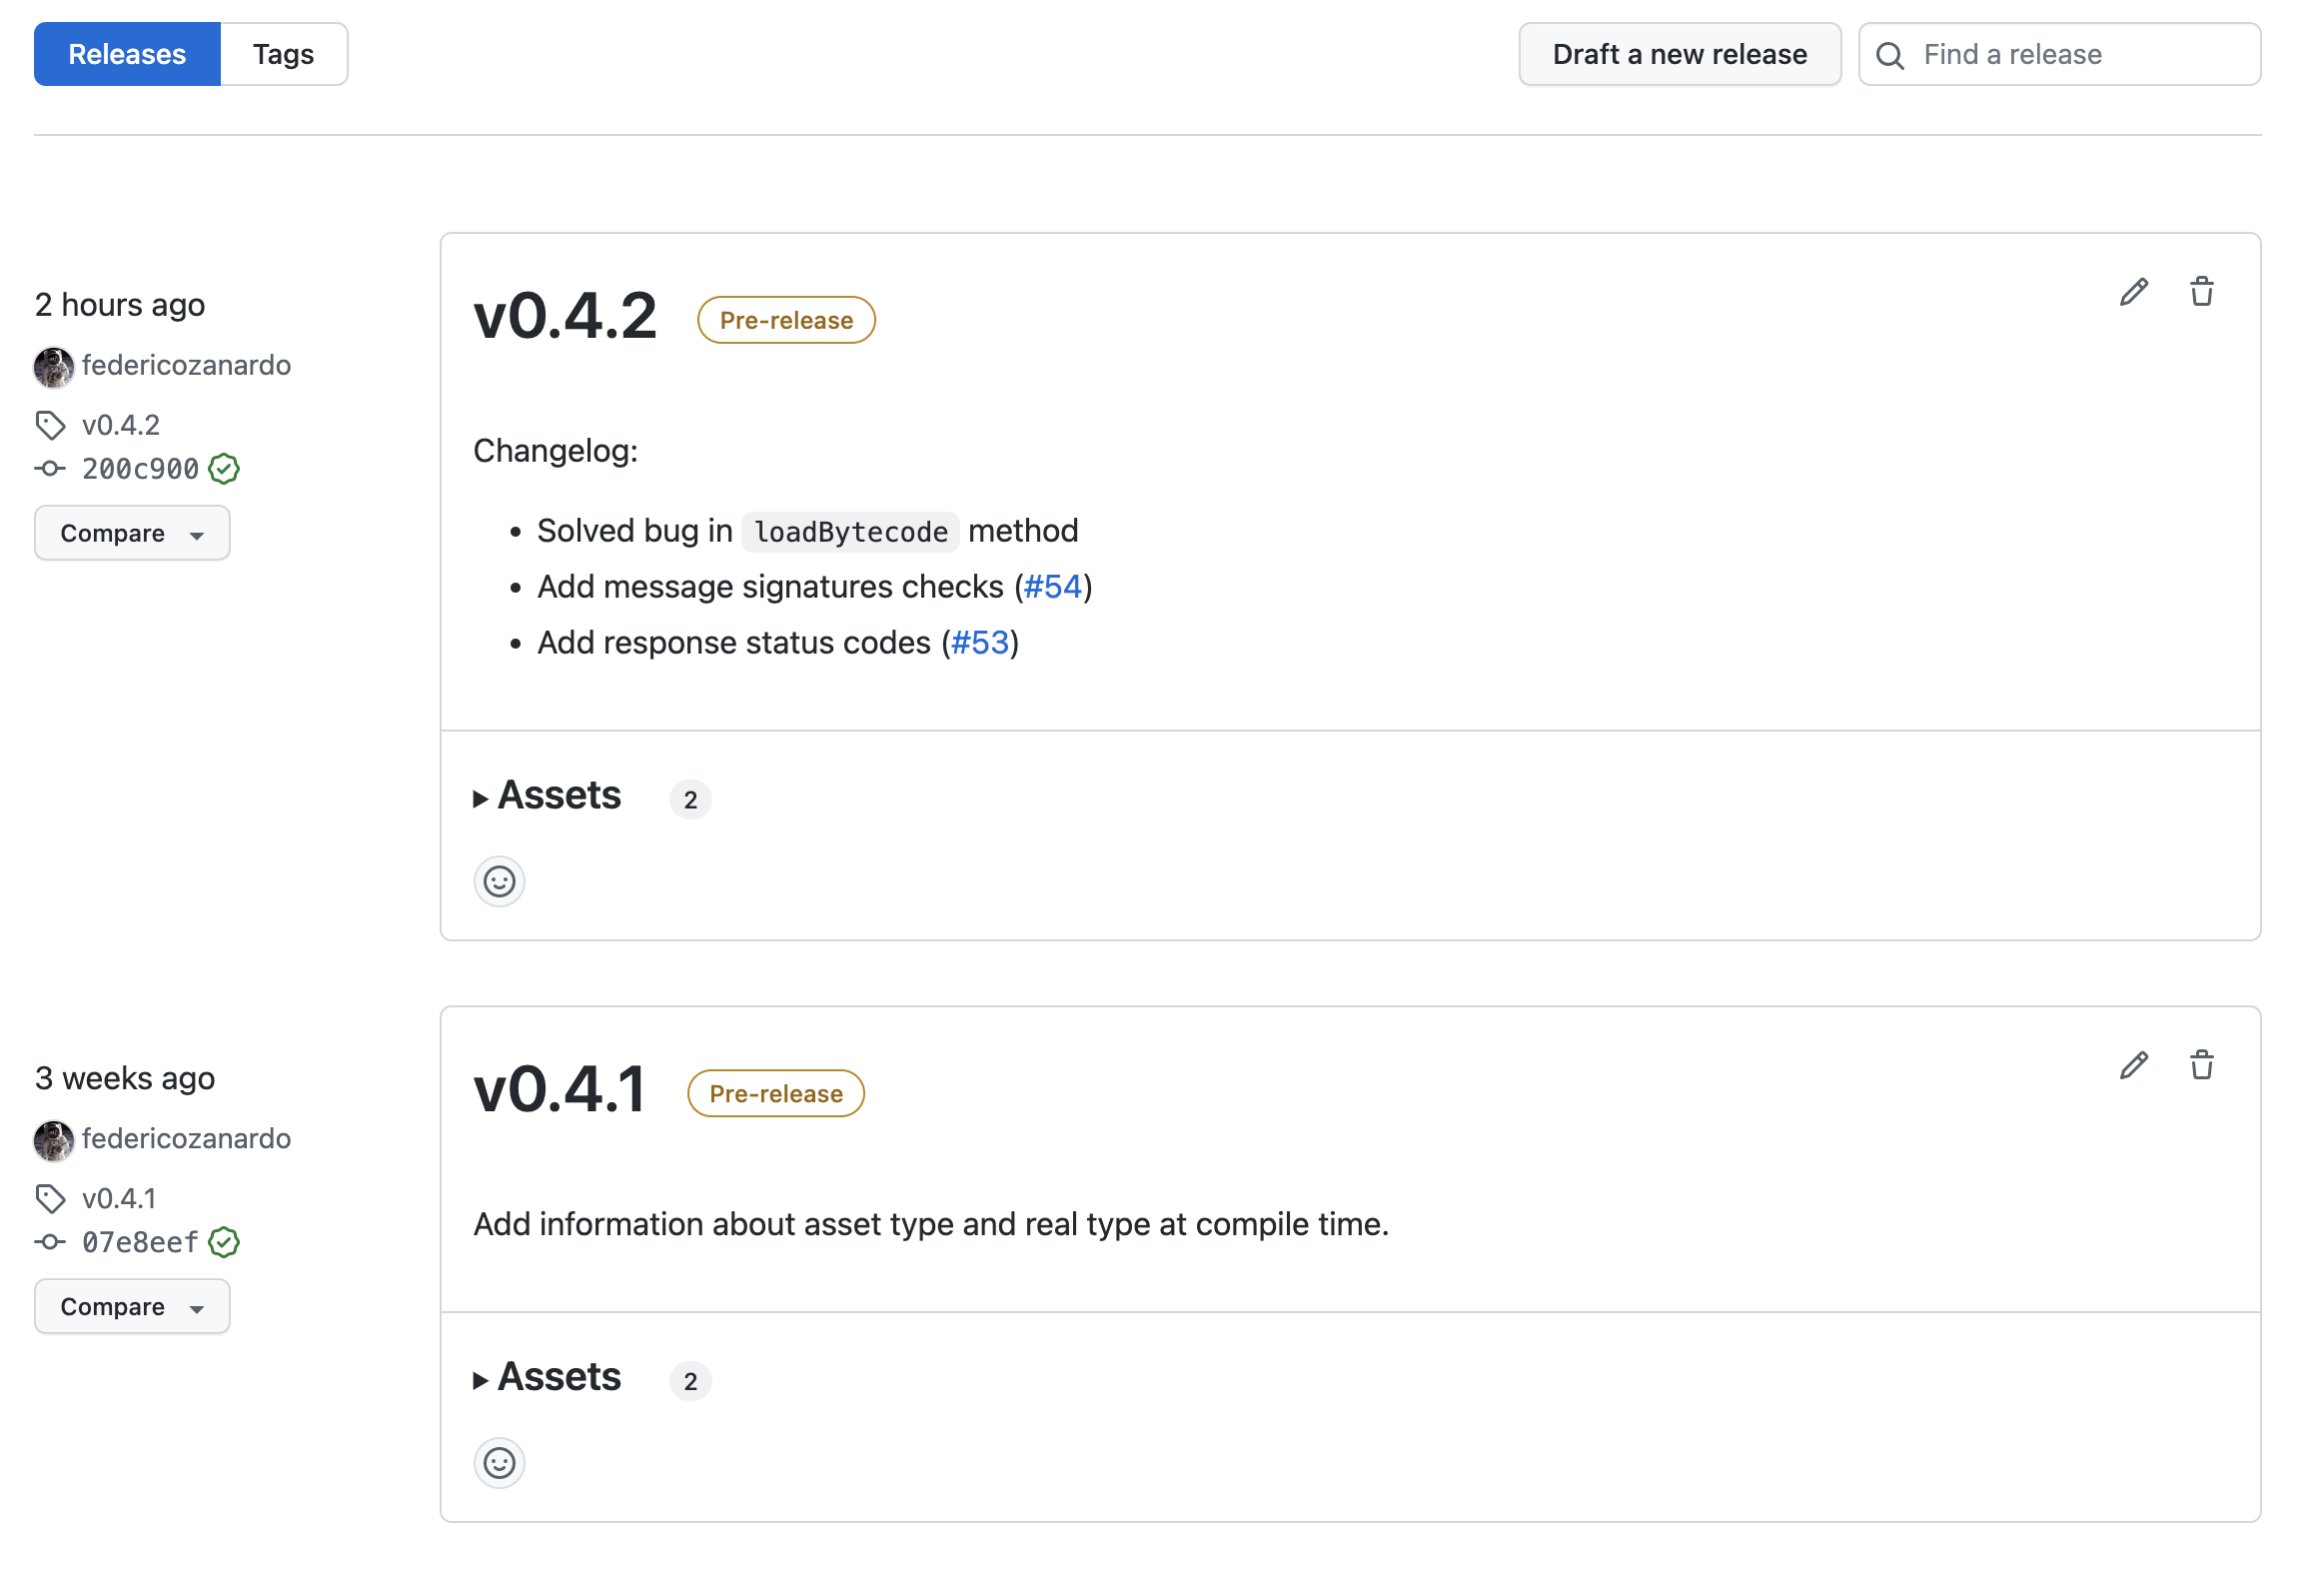
\includegraphics[width=0.9\textwidth]{immagini/capitolo-5/releases.png}
		\caption{Various project releases. For each release it is possible to download the code and start an 
    instance of \textit{Stipula}.}
		\label{fig:releases}
	\end{center}
\end{figure}

\begin{figure}[htbp]
	\begin{center}
		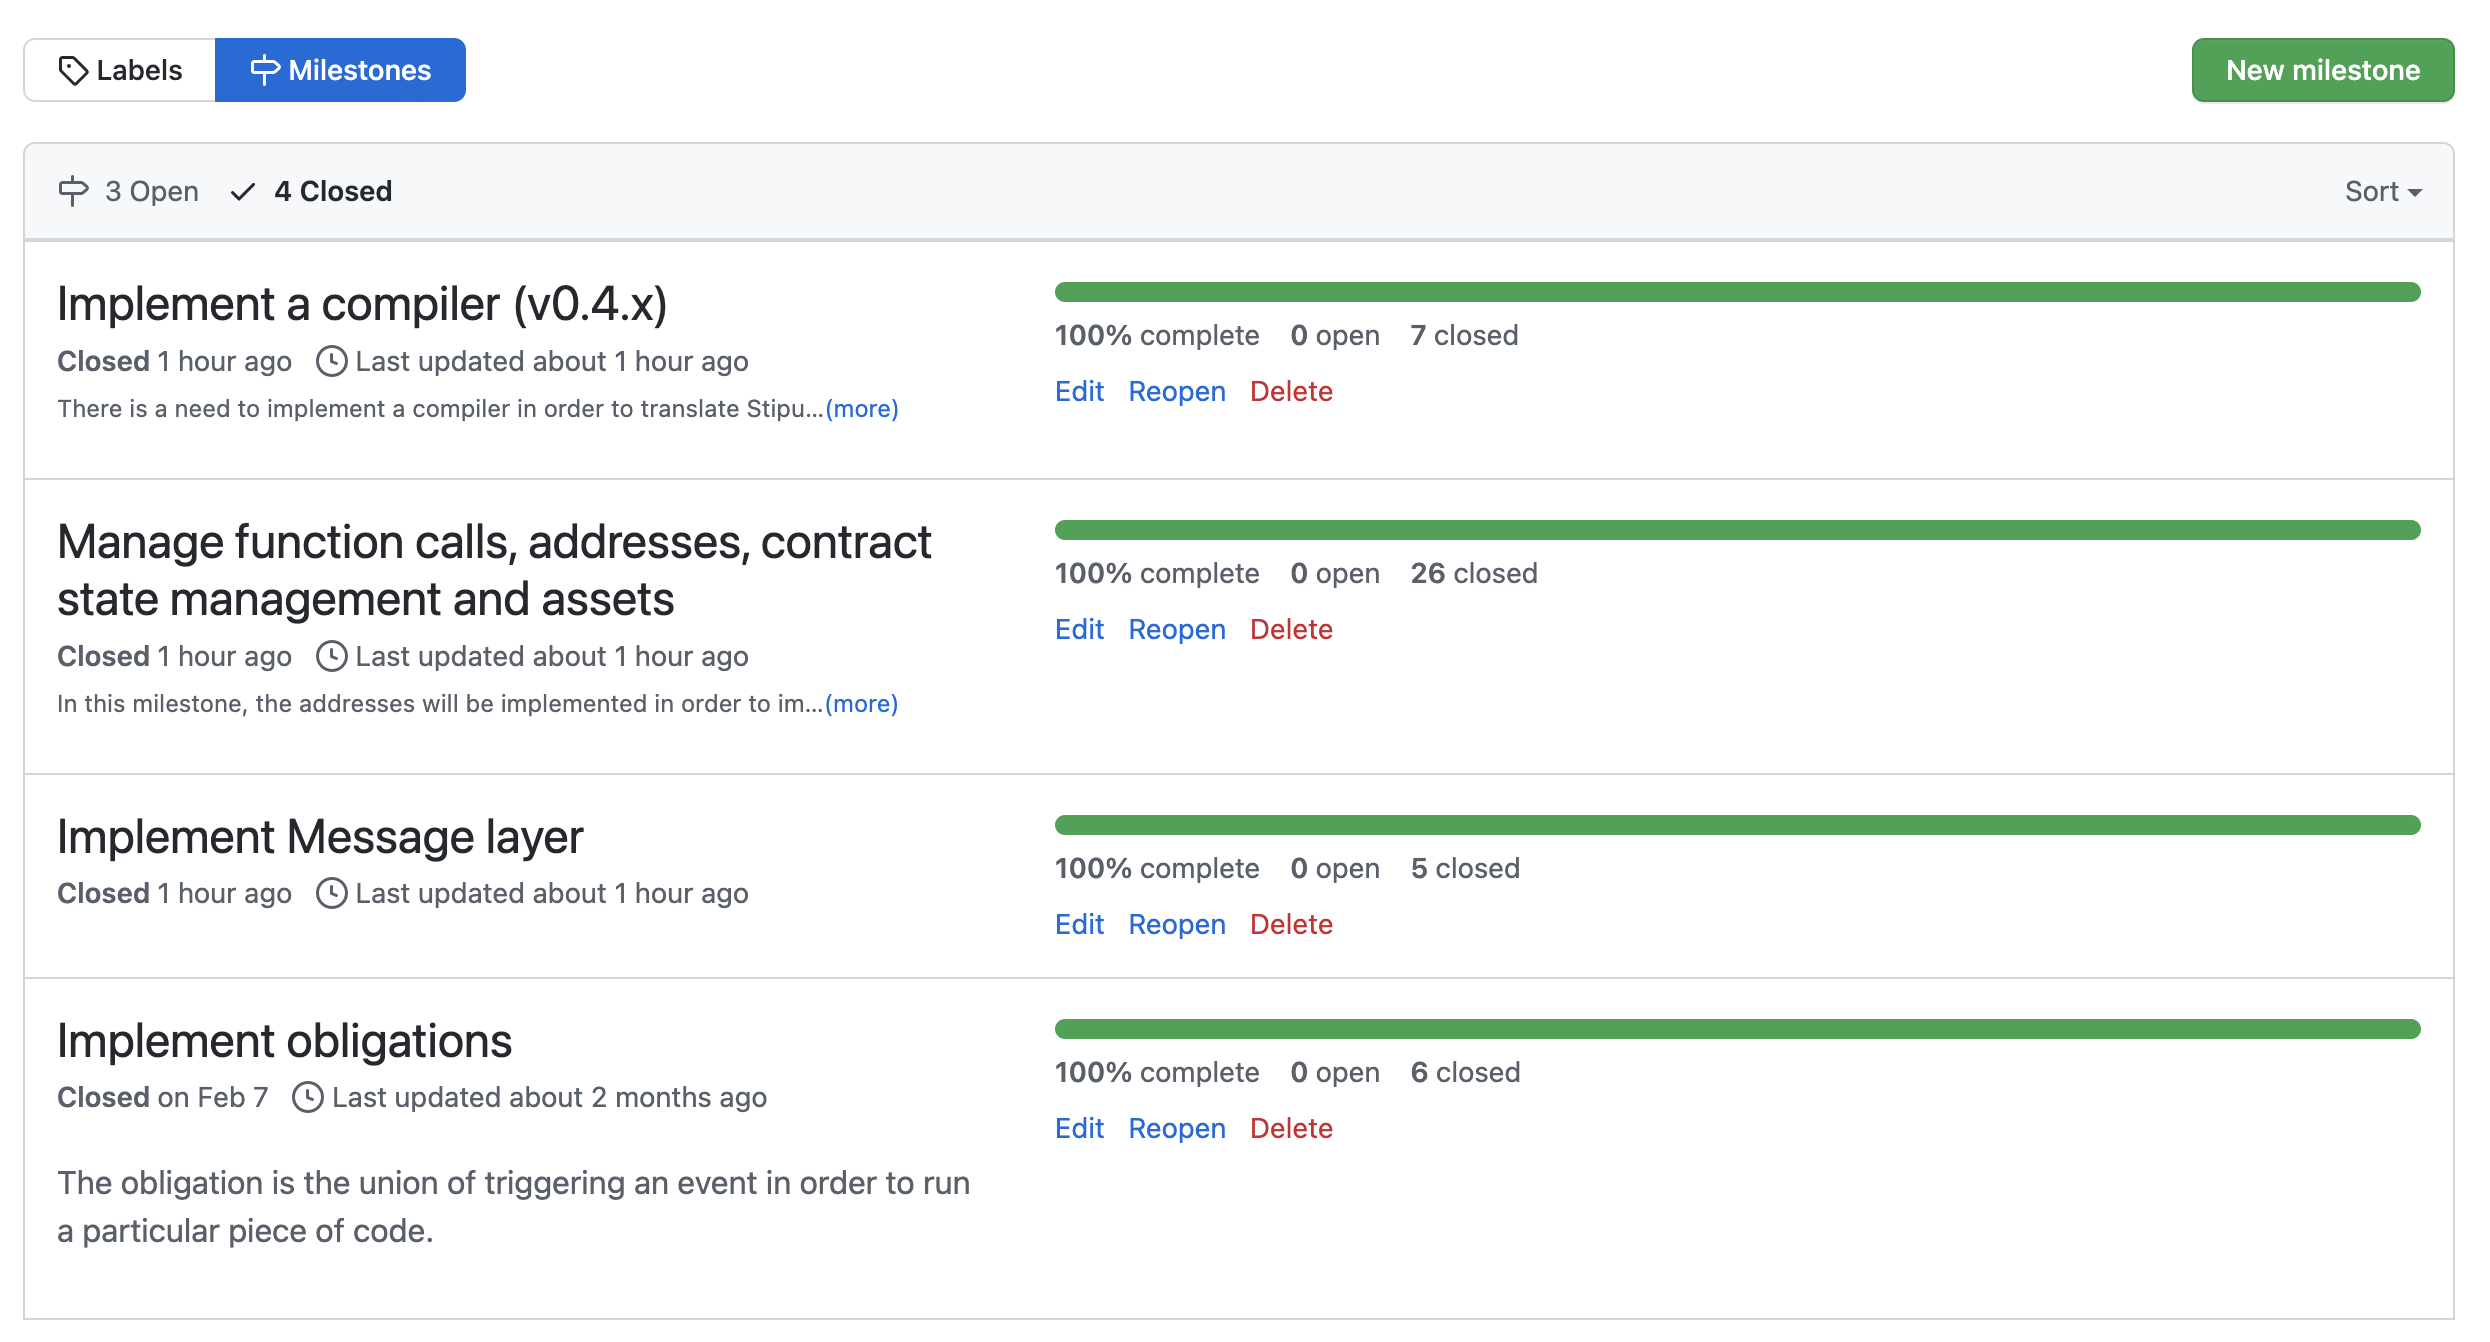
\includegraphics[width=0.9\textwidth]{immagini/capitolo-5/milestones-closed.png}
		\caption{Milestones completed.}
		\label{fig:milestones-closed}
	\end{center}
\end{figure}

\begin{figure}[htbp]
	\begin{center}
		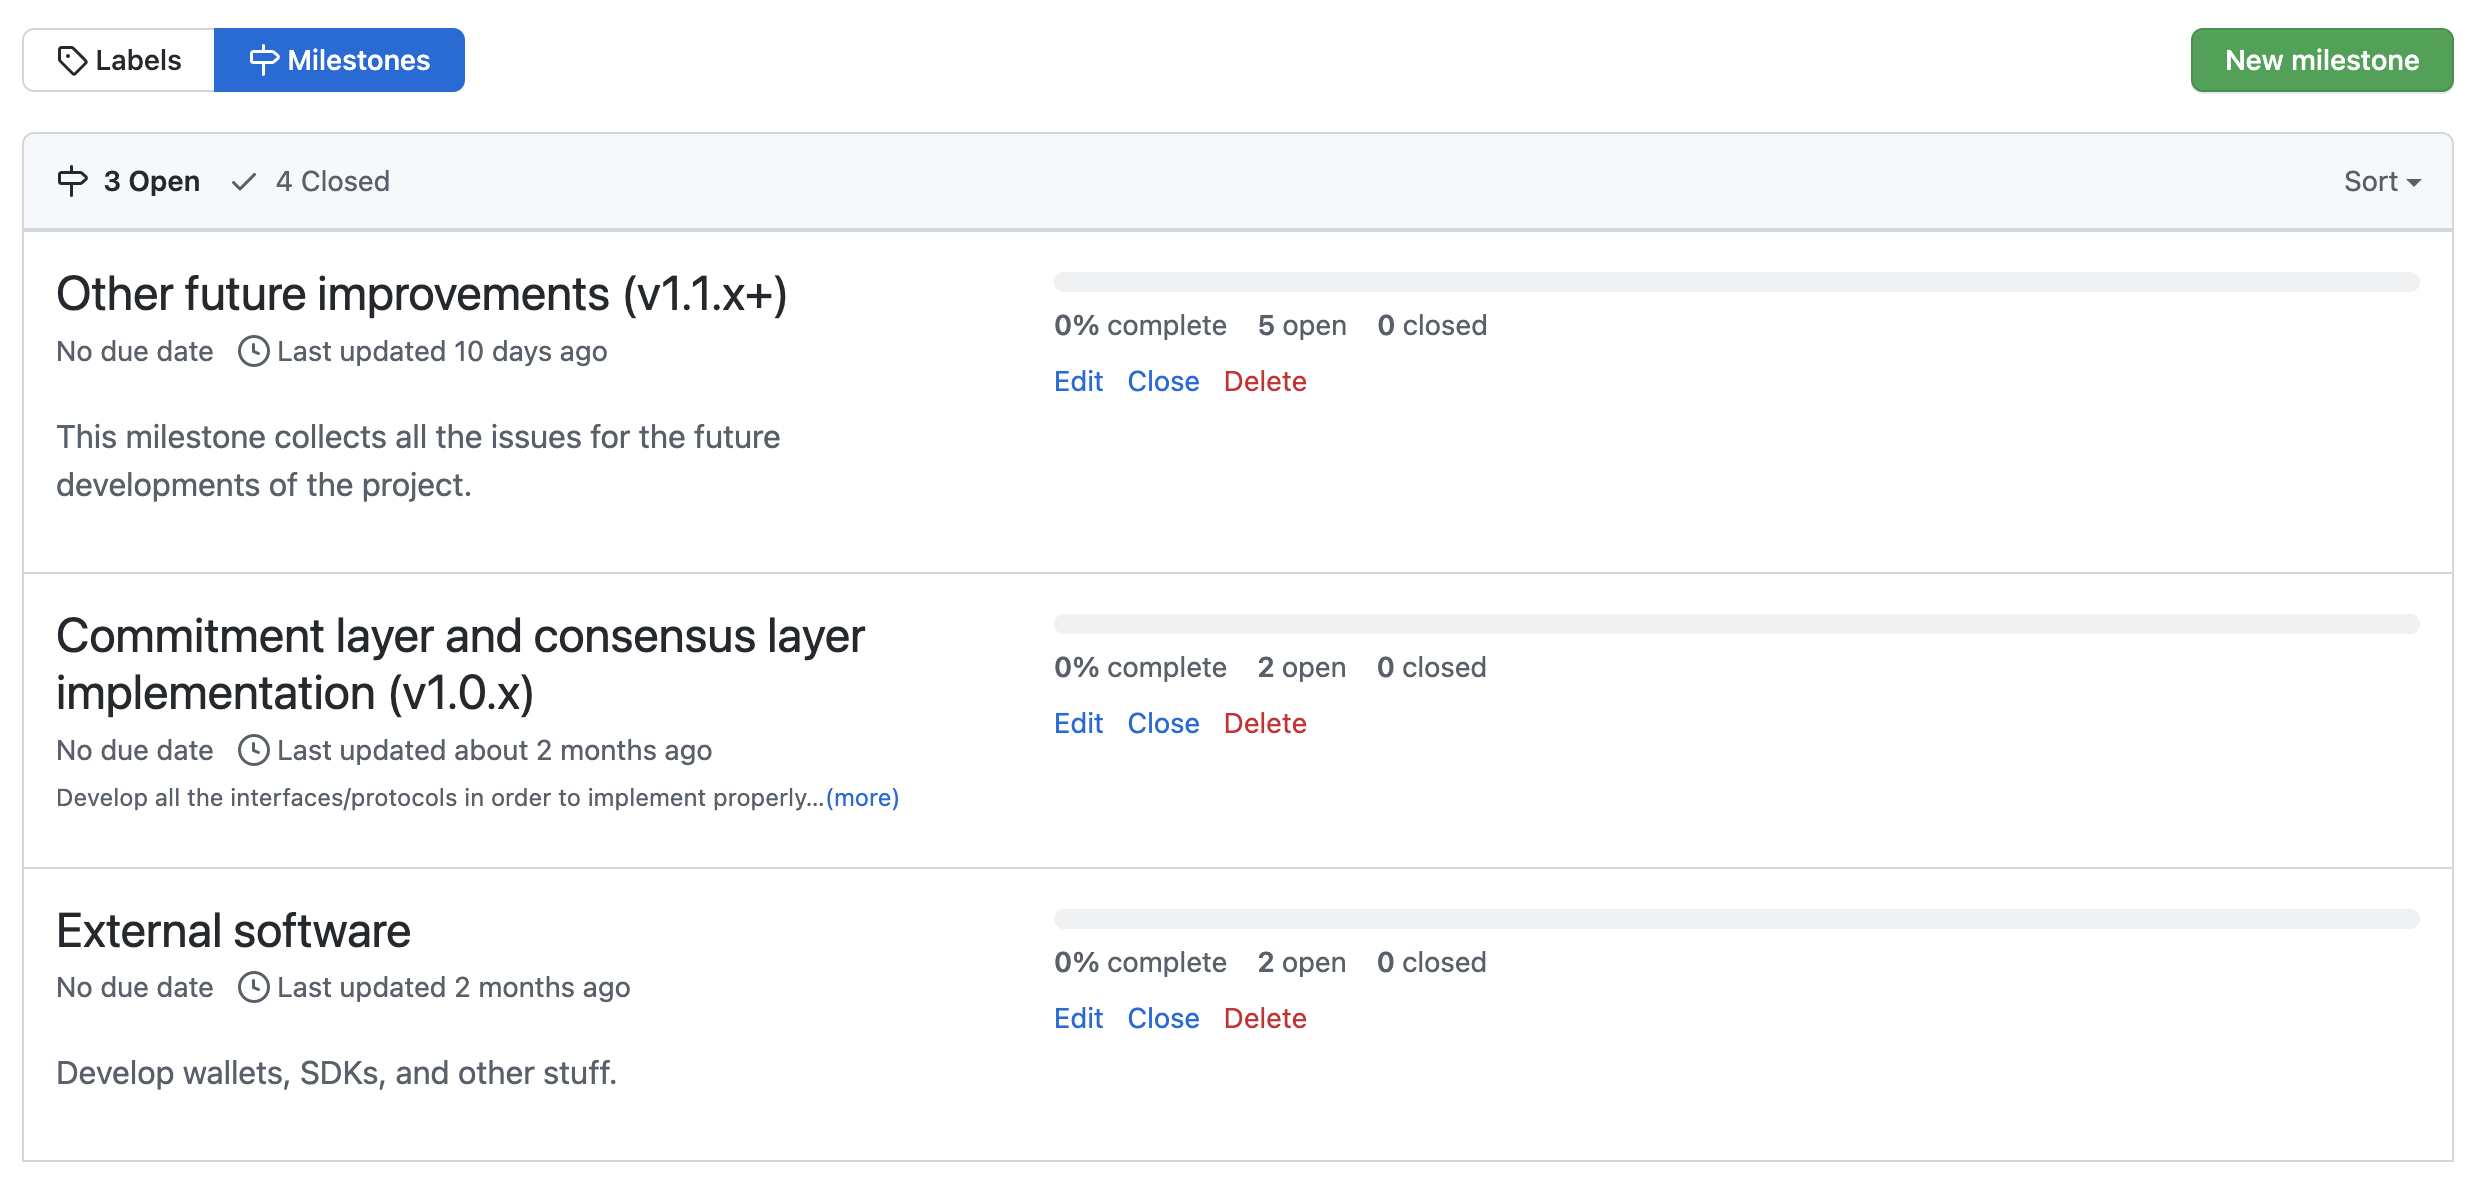
\includegraphics[width=0.9\textwidth]{immagini/capitolo-5/milestones-opened.png}
		\caption{Milestone opened.}
		\label{fig:milestones-opened}
	\end{center}
\end{figure}

\subsection{Installation}

Starting a \textit{Stipula} server can be done by downloading the code and installing all the packages, or 
by downloading a Docker image and running the container. For manual installation, you need:
\begin{enumerate}
  \item Java SDK 8
  \item Gradle 7.6.0
  \item Gson 2.10.1 
  \item LevelDb 0.9
  \item ANTLR 4.10
  \item JUnit 5.8.1
\end{enumerate}

The \ref{app:gradle} appendix contains the code of the \verb|build.gradle| file, which allows you to 
install and manage the project packages.

For a faster and easier to manage installation it is better to use a Docker image. You can create an 
instance of \textit{Stipula} with Docker in two ways:
\begin{enumerate}
  \item Download the project and run \verb|docker build -t stipula-node:<version> .|, where you must 
  specify the version you want to use instead of \verb|<version>|. You also specify the version in the 
  \verb|docker-compose.yml| file and execute the command \verb|docker-compose -f docker-compose.yml up -d|;
  \item Download the Docker files and specify in the \verb|docker-compose.yml| file that the image you 
  want to use must be downloaded from a particular page \autocite{site:stipula-github-available-packages}, 
  that is, \verb|image: "ghcr.io/federicozanardo/stipula-node:<version>"|. To start the container, use 
  the command \verb|docker-compose -f docker-compose.yml up -d|.
\end{enumerate}

The benefit you get is that you can run an instance on any machine that supports Docker and takes the 
responsibility off managing package updates.

Furthermore, each Docker image available at the address 
\begin{Verbatim}
  ghcr.io/federicozanardo/stipula-node:<version>
\end{Verbatim}
is an image that is created at each new release, to which it is obviously subjected to tests. In the 
appendix \ref{app:docker} there is the code of the \verb|Dockerfile| and \verb|docker-compose.yml|.

\label{database-seeding}
Due to the limitations of the implemented architecture, to carry out tests and demonstrate the 
functioning of the implemented implementation, there is the need to initialize assets and 
single-use-seals for addresses. To do this, it is necessary to set the \verb|SEED| environment variable: 
by setting \verb|yes|, assets and single-use-seals will be created when the program is started; valuing 
with \verb|no|, this procedure will not be performed. The enhancement of this environment variable can be 
done inside the \verb|docker-compose.yml| (line 12). The following chapter will illustrate the limits of 
this architecture and propose solutions. In the future, this database \textit{seeding} procedure will be 
removed.
	        % Implementation
% !TEX encoding = UTF-8
% !TEX TS-program = pdflatex
% !TEX root = ../tesi.tex

%**************************************************************
\chapter{Missing features and future developments}
\label{cap:future-developments}
%**************************************************************.

This chapter will illustrate the missing features, the limitations of the implemented architecture, the 
possible optimizations that can be implemented and future developments for the project as a whole.

%**************************************************************

\section{Missing features}

In this section we introduce the missing features for a complete implementation of the \textit{Stipula} 
language. The reason for the lack of these features is not due to a limitation of the built architecture, 
but due to a lack of time to implement them.

\subsection{Language features not implemented in the current version}

The language offers several features for writing contracts. Many of these features require certain 
properties to be guaranteed, which are often complex to maintain. In the architecture illustrated above, all 
the features of the language have been implemented, except one: the sending of messages from the contract to 
the customer. The original example of the \verb|BikeRental| contract (see section 
\ref{bike-rental-example-definition}) foresaw:
\begin{enumerate}
  \item When the user called the \verb|accept| function, the bicycle code was sent to the customer. In 
  particular, the complete code would have been:
  \label{send-use-code}
  \begin{Verbatim}[numbers=left,xleftmargin=2cm,firstnumber=14]
    ...
    @Proposal Borrower : accept()[y]
        (y == cost) {
            y -o wallet;
            use_code -> Borrower
            ...
  \end{Verbatim}
  \item When the \verb|accept| function is required was executed, the contract would notify the customer of 
  the end of the service, by sending the \verb|"End_Reached"| message. In particular, the complete code 
  would have been:
  \label{trigger-event-with-message}
  \begin{Verbatim}[numbers=left,xleftmargin=2cm,firstnumber=18]
    ...
    now + rentingTime >>
      @Using {
        "End_Reached" -> Borrower
        wallet -o Lender
      } => @End
    ...
  \end{Verbatim}
\end{enumerate}

The architecture is ready to implement this feature, that is, the infrastructure for communication between 
the virtual machine and the client has already been implemented. The missing part is figuring out the 
necessary data structures and response messages to send to the client.

\label{syntactic-sugar}
Due to time constraints, it was not possible to implement the \textit{syntactic sugar} required by the 
language. The language expects the following syntactic sugar:
\begin{enumerate}
  \item 
  \begin{Verbatim}[xleftmargin=2cm]
    ...
    @State1,@State2 Party1,Party2 : functionName()[]
    ...
  \end{Verbatim}

  That is, allowing a specific function to be called from multiple parties and/or from multiple states. The 
  implementation of this syntactic sugar involves both the compiler and the virtual machine: the compiler 
  must produce optimized bytecode, that is, instead of writing the function body for each state and for each 
  party, one could update the bytecode language to notify the virtual machine that that code can be invoked 
  from different parties and in different states. The benefits would be obtained from the point of view of 
  memory, as it would be possible to save space instead of duplicating the body of the function each time. 
  In a distributed context, this represents an important point, because it is important to minimize memory 
  usage as much as possible. It is necessary to clarify this is a pure consideration from the point of 
  view of optimization and not from the point of view of expressiveness. The lack of this syntactic sugar 
  does not diminish the expressiveness of the language: in fact, it is possible to write the same function 
  code several times in the bytecode with different states and callers. However, the implementation of 
  this syntactic sugar was not possible due to lack of time.
  \item See \cite{site:stipula-programming-legal-contracts}
  \begin{Verbatim}[xleftmargin=2cm]
    ...
    ~ @End _ : block(x) {
      x -> _
    } ==> @Exception
    ...
  \end{Verbatim}

  Similarly to the previous point, the implementation of this syntactic sugar involves the compiler and the 
  virtual machine. The meaning of this code is as follows: the \verb|block| function can be invoked by any 
  party ("\verb|_|" notation) provided that the duration of the contract has not expired, that is, the 
  contract is not in the \verb|@End| state.
\end{enumerate}

\subsection{Single-use-seals merge}
\label{single-use-seals-merge}

The current version has an important limitation when the user has to make a payment to an instance of a 
contract. In order to make a payment, the user must have available a single-use-seal of the exact quantity 
required by the contract: if the user does not have a single-use-seal of the requested quantity, the user 
cannot make the payment. This problem represents a strong limit to be able to massively use this 
implementation. One proposed solution is to \textit{merge} single-use-seals. Suppose Alice has to pay the 
contract \verb|C_1| 15 \verb|StipulaCoin|. Alice has the following single-use-seals available (note the 
image \ref{fig:single-use-seals-merge}):
\begin{enumerate}
  \item Single-use-seal 1 (\verb|S_1|): 5 \verb|StipulaCoin|;
  \item Single-use-seal 2 (\verb|S_2|): 7 \verb|StipulaCoin|;
  \item Single-use-seal 3 (\verb|S_3|): 2 \verb|StipulaCoin|;
  \item Single-use-seal 4 (\verb|S_4|): 2 \verb|StipulaCoin|;
\end{enumerate}

\begin{figure}[htbp]
	\begin{center}
		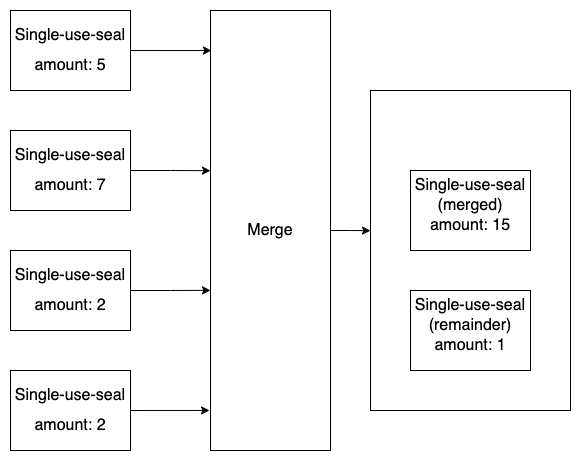
\includegraphics[height=7cm]{immagini/capitolo-6/single-use-seals-merge.png}
		\caption{Example of single-use-seals merge.}
		\label{fig:single-use-seals-merge}
	\end{center}
\end{figure}

In the current version Alice could not pay the contract as she does not have a single-use-seal of 15 
\verb|StipulaCoin|, however the sum of all available funds is 16 \verb|StipulaCoin|, enough to be able to 
carry out the transaction. The proposed solution consists first of all in modifying the message to make 
function calls (see \ref{function-call-message}), specifically when a \textit{Pay-to-Contract} must be 
made. The message must be able to collect multiple single-use-seals in its payload. More precisely:
\begin{enumerate}
  \item \verb|unlockScript| must be provided for each single-use-seals, so that the user proves ownership of 
  the funds;
  \item Create new single-use-seals:
  \begin{enumerate}
    \item One represents the single-use-seal that will be sent to the contract (\verb|merged|); % line 58
    \item The other single-use-seal represents the \textit{remainder} (\verb|remainder|), that is, 
    the difference between the sum of all the single-use-seals in input minus the amount of asset needed to 
    contract. % line 72
  \end{enumerate}
\end{enumerate} 

I single-use-seals \verb|merged| and \verb|remainder| are the new single-use-seals that will need to be 
stored. The identifier of these single-use-seals is computed from the hash of the input single-use-seals 
identifiers. The reason is to decrease the probability of collision between the identifiers of the other 
single-use-seals. The \verb|merged| must be sent with the contract and therefore \verb|unlockScript| must be 
provided, to demonstrate possession of the single-use-seal. Instead, you don't need to supply 
\verb|unlockScript| for the \verb|remainder|, as it is not to be spent in this transaction.

An example is shown below:

\begin{enumerate}
  \item Line 5 specifies that the payment is a \textit{single-use-seal merge} (\verb|merge|). From line 8 
  to line 29, all single-use-seals that Alice wants to merge are specified. You can see that for each 
  single-use-seal, Alice has provided cryptographic proof of ownership of those funds. In particular, on 
  line 12, 17, 22, 27 it is possible to note the presence of the \verb|unlockScript| field.

  For \verb|<ownershipId_S_1>| we refer to the identifier of the \textit{first} single-use-seal that Alice 
  wants to spend and for \verb|<unlockScript_S_1>| refers to the \verb|unlockScript| del \textit{first} 
  single-use-seal. The same goes for \verb|<ownershipId_S_2>|, \verb|<ownershipId_S_3>|, 
  \verb|<ownershipId_S_4>|, \verb|<unlockScript_S_2>|, \verb|<unlockScript_S_3>| and 
  \verb|<unlockScript_S_4>|
  \begin{Verbatim}[numbers=left,xleftmargin=1cm,firstnumber=1,breaklines=true,tabsize=2]
    ...
    "arguments": [
      {
        "argument": {
          "first": "merge",
          "second": "y",
          "third": {
            "input": [
              {
                "ownershipId": "<ownershipId_S_1>",
                "address": "<Alice_address>",
                "unlockScript": "<unlockScript_S_1>"
              },
              {
                "ownershipId": "<ownershipId_S_2>",
                "address": "<Alice_address>",
                "unlockScript": "<unlockScript_S_2>"
              },
              {
                "ownershipId": "<ownershipId_S_3>",
                "address": "<Alice_address>",
                "unlockScript": "<unlockScript_S_3>"
              },
              {
                "ownershipId": "<ownershipId_S_4>",
                "address": "<Alice_address>",
                "unlockScript": "<unlockScript_S_4>"
              }
            ],
  \end{Verbatim}

  \item From line 30 to line 56, it is possible to notice what is the output of the merger of the previous 
  single-use-seals (\verb|output|). From line 31 to line 45, you can see the specification of the new 
  single-use-seal \verb|merged|, which will be sent to the contract instance to make the payment. In fact, 
  this new single-use-seal already comes with the \verb|unlockScript| (line 43). By doing so, the contract 
  will be able to verify whether these funds will actually belong to Alice or not. Instead, from line 46 
  to line 56, it is possible to notice that a new single-use-seal (\verb|remainder|) is created which 
  represents the difference between the sum of all single-use-seals specified in \verb|input | minus the 
  amount of assets required by the contract instance. No \verb|unlockScript| needs to be supplied for this 
  single-use-seal because it must not be spent on this payment.

  For \verb|<hash(ownershipId_S_1)>| means the hash of the identifier of the first input single-use-seal 
  and for \verb|<unlockScript_hash(ownershipId_S_1)>| means the \verb|unlockScript| of this new 
  single-use-seal with identifier \verb|<hash(ownershipId_S_1)>|. The same goes for the single-use-seal 
  \verb|remainder|
  \begin{Verbatim}[numbers=left,xleftmargin=1cm,firstnumber=57,breaklines=true,tabsize=2]
      "output": {
        "merged": {
          "single_use_seal": {
            "asset_id": "stipula_coin_345",
            "amount": {
              "value": "1500",
              "decimals": "2"
            }
          },
          "ownership": {
            "ownershipId": "<hash(ownershipId_S_1)>",  
            "address": "<Alice_address>",
            "unlockScript": "<unlockScript_hash(ownershipId_S_1)>"
          }
        },
        "remainder": {
          "single_use_seal": {
            "asset_id": "stipula_coin_345",
            "amount": {
              "value": "100",
              "decimals": "2"
            }
          }
        }
      }
  \end{Verbatim}
\end{enumerate}

Let's illustrate the complete example:
\label{single-use-seal-merge-example}
\begin{Verbatim}[numbers=left,xleftmargin=1cm,firstnumber=1,breaklines=true,tabsize=2]
  ...
    "arguments": [
      {
        "argument": {
          "first": "merge",
          "second": "y",
          "third": {
            "input": [
              {
                "ownershipId": "<ownershipId_S_1>",
                "address": "<Alice_address>",
                "unlockScript": "<unlockScript_S_1>"
              },
              {
                "ownershipId": "<ownershipId_S_2>",
                "address": "<Alice_address>",
                "unlockScript": "<unlockScript_S_2>"
              },
              {
                "ownershipId": "<ownershipId_S_3>",
                "address": "<Alice_address>",
                "unlockScript": "<unlockScript_S_3>"
              },
              {
                "ownershipId": "<ownershipId_S_4>",
                "address": "<Alice_address>",
                "unlockScript": "<unlockScript_S_4>"
              }
            ],
            "output": {
              "merged": {
                "single_use_seal": {
                  "id": "<hash(S_1)>",
                  "asset_id": "stipula_coin_345",
                  "amount": {
                    "value": "1500",
                    "decimals": "2"
                  }
                },
                "ownership": {
                  "ownershipId": "<hash(ownershipId_S_1)>",  
                  "address": "<Alice_address>",
                  "unlockScript": "<unlockScript_hash(ownershipId_S_1)>"
                }
              },
              "remainder": {
                "single_use_seal": {
                  "id": "<hash(S_2)>",
                  "asset_id": "stipula_coin_345",
                  "amount": {
                    "value": "100",
                    "decimals": "2"
                  }
                }
              }
            }
          }
        }
      }
    ],
    ...
  }
  ...
}
\end{Verbatim}

This solution allows you to make payments even if you don't have single-use-seals of the precise quantity 
required by the contract. The solution requires updating the message format and carrying out further 
preliminary checks before executing the contract, namely:
\begin{enumerate}
   \item Checking the single-use-seals of inputs: in addition to verifying ownership via the 
   \textit{Script}, it is also necessary to check that the sum of the inputs is greater than or equal to the 
   quantity required by the contract;
   \item Controlling single-use-seals \verb|merged| and optionally \verb|remainder|: verify that the sum of 
   the quantities of the input single-use-seals is equal to the sum of the quantities of \verb|merged| and 
   optionally \verb|remainder|. Also, verify that the single-use-seal \verb|merged| is equal to the quantity 
   required by the contract;
\end{enumerate}

Passing these checks, the input single-use-seals will be updated in \textit{Storage} as spent. The 
single-use-seals \verb|merged| will be stored in storage directly as spent, while the single-use-seal 
\verb|remainder| is stored as unspent. At this point, the virtual machine can continue with the execution of 
the contract.

\subsection{Creation of assets and their distribution}
\label{creation-assets-and-distribution}

One of the missing aspects in the current version is the ability to create additional assets beyond the 
hard-coded one. As an example, hard-coded assets have been created for the implemented version. One of the 
peculiarities of the \textit{Stipula} language is that of being able to schedule the execution of certain 
obligations over time. This functionality could be leveraged to manage the creation, issuance and 
destruction of assets. The creation of an asset should take place by means of a special contract, separate 
from the classic contracts seen above. In this special contract, the maximum supply, the fractionability of 
the asset, the name and an identifier would be defined. However, an asset issuance mechanism could also be 
defined, such as the \textit{halving} for Bitcoin ((see \cite{site:bitcoin-mining}, 
\cite{site:bitcoin-halving} and \cite{book:mastering-bitcoin})): using the scheduling of events over time, it is possible 
to establish that periodically a certain amount of assets is entered into the system. Furthermore, it is 
also possible to define addresses for the \textit{burn} of the assets. Burning an asset is used to remove 
liquidity from circulation, thereby decreasing available supply and appreciating the asset. If you want to 
burn a certain amount of assets, you send it to a specific address where you can only deposit and not 
withdraw. In this way, it is also possible to monitor and verify the amount of burned assets.

\newpage
\section{Optimizations}
\label{optimizations}

The current architecture has mainly two bottlenecks:
\begin{enumerate}
  \item \textit{Virtual Machine}: requests to execute function calls of an instance of a contract or the 
  execution of a time-scheduled event are computed \textit{sequentially};
  \item \textit{Storage}: for simplicity in the realization of the implementation, each request, both for 
  reading and for writing, is managed by a \textit{mutex}, to guarantee exclusive access to the memory by a 
  superior module .
\end{enumerate}
Requests addressed to the compiler and requests addressed to the virtual machine are handled in parallel 
until one has to interact with the \textit{Storage} module.

\subsubsection{Virtual Machine}

Requests directed to the virtual machine are done \textit{sequentially}. Unfortunately, this implementation 
choice represents a bottleneck as regards system performance, in particular, precisely for the virtual 
machine, which is the most used module during the execution of a contract. However, it is possible to 
implement optimizations, paying attention, however, to avoid cases of competition. Some possible 
optimizations for the virtual machine are:
\begin{enumerate}
  \item \textit{Parallelization of single-use-seals}: this is possible thanks to the UTXO model used in the 
  architecture. The operation of this property has been described \ref{utxo-parallelization}. For example: 
  Alice has two single-use-seals \verb|S_1| and \verb|S_2| and she wants to make two payments to two 
  different contracts \verb|C_1| and \verb|C_2|. With this optimization, Alice can pay the \verb|C_1| 
  contract with \verb|S_1| and \verb|C_2| with \verb|S_2|. The two requests can be run in parallel because 
  they use separate funds and there is no need to run either request first to update the asset balance, as 
  might be the case in an account-balance-based model. The same dynamic would also occur if Alice had to 
  pay two different instances of the same contract or two instances of two different contracts;
  \item \textit{Parallelization of function calls}: if a user is interacting with multiple instances of 
  contracts at the same time, the requests can be executed in parallel. If multiple users are interacting 
  with the same instance of a contract, requests will be fulfilled in order of arrival. As regards the 
  execution of obligations (events scheduled over time), the basic principle does not change: the event 
  can be parallelized if the other requests interact in different contract instances, otherwise the 
  execution of the event has priority over the execution of function calls.
\end{enumerate}

These optimizations can significantly increase the \textit{throughput} of requests, especially in a 
distributed context. However, it is necessary to update the structure of some modules and to pay particular 
attention to concurrency.

\subsubsection{Storage}

Requests received by this module could be parallelized by splitting them into \textit{read} and 
\textit{write} requests. Requests can come from the compiler, from the virtual machine or directly from the 
\textit{Message Service}. If the module is only receiving read requests, these requests can be executed in 
parallel; when a write request is received, it takes priority over read requests. As a further optimization, 
you could make a specific resource exclusive when a write request is received, and leave free access to 
other resources.

\section{Limits of the architecture}

\subsection{Computational and memory resources required}

One of the factors to increase the decentralization of a network is to allow the creation of nodes that 
have a low computational capacity and limited storage capacity. If a ledger were to require large 
computational capabilities and large amounts of memory, this implies that more expensive machines would be 
needed. The need for more expensive machines increases the centralization of the network, as the subjects 
who will be able to buy and maintain these machines will be limited in number. Therefore, in the design 
phase it is also important to take into account the computational and memory aspect. One of the most 
expensive operations in a decentralized network is the \textit{synchronization} of the nodes. If the ledger 
used a lot of memory, this would increase the time it takes to synchronize, thus increasing the possibility 
of transmission errors. Obviously, this phase would be much more complex and difficult to complete for 
devices with limited computational and memory capabilities. The current implementation stores various 
information in the \textit{Storage} module. This could pose a problem for especially distributed networks, 
if decentralized. During the development of the project we focused on saving all the information necessary 
to allow the execution of the contracts and for the management of the asset transfers. It would be necessary 
to analyze whether all the information that is currently stored is actually necessary or, on the other hand, 
it is possible to omit some information because it is possible to deduce it from other information. 
Obviously, this balance must be calibrated correctly with the computational cost required to retrieve this 
information: if it is possible to save a minimal set of information that is currently stored, but the 
operations necessary to retrieve it require a considerable increase in computational resources, this 
represents one downside. Furthermore, for simplicity and for a limited amount of time available, the 
information has been stored according to the data structures of Java objects, as the \textit{LevelDB} 
library allows information to be stored in bytes. A necessary development is to create information storage 
interfaces for the various storages (\textit{contracts}, \textit{contract-instances}, \textit{assets} and 
\textit{ownerships}), in order to allow to implement nodes also in other programming languages.

From a computational point of view, the current version of the language is not Turing-complete, so it is not 
possible to loop and make function calls from other functions. This design choice limits the expressiveness 
of the language and therefore also limits the possibility of creating programs that may require significant 
computational resources. The \textit{Script} language is also not Turing-complete, so it is possible to 
create programs that require little computational resources. Furthermore, non-Turing-completeness also 
allows you to avoid unwanted behavior and prevent potential security vulnerabilities. In the previous 
section (\ref{optimizations}), possible optimizations were introduced to increase request throughput. These 
optimizations must also take into consideration devices that have limited computational capacity: in this 
case it is preferable to implement certain optimizations and others not, obtaining a lower throughput for 
greater decentralization. Obviously, these considerations refer exclusively to decentralized networks.

\newpage
\section{Current version security issues}

One of the key principles that guided the entire development is security from various points of view. In 
fact, security can be understood as regards:
\begin{enumerate}
   \item The assets, that is, guaranteeing that the transfer of assets between users and contracts, and vice 
   versa, takes place without loss of quantity or generation of new quantities from scratch;
   \item Prevent a user from double-spending;
   \item Ensure that after a contract is executed, the correct state is reached.
\end{enumerate}

The architecture presented above has a security problem regarding the transmission of messages between the 
server/node and the client. The attack that might occur is a \textit{Man-In-The-Middle} (\textit{MITM}) 
attack. When a user wants to send a message to the \textit{Stipula} server/node, the message is signed. The 
benefits of signing are:
\begin{enumerate}
   \item \textit{Authentication}: the recipient can verify that the message was sent by the declared sender, 
   since only the sender has the private key to sign the message;
   \item \textit{Integrity}: the recipient can be certain that the message has not been tampered with during 
   transmission, as any alteration of the message would invalidate the signature;
   \item \textit{Non-repudiation}: the sender cannot deny having sent the message once signed, since the 
   signature provides verifiable proof of authorship.
\end{enumerate}

Thus, when the \textit{Stipula} server/node receives a message, even if it is not encrypted, the sender has 
expressed his intentions of wanting to create a new instance of a contract or make a function call. However, 
when it is the \textit{Stipula} server/node that has to send response messages to the client, these can be 
intercepted and tampered with. Indeed, in the server/node there are no cryptographic keys that certify the 
authenticity and integrity of a message. The problems of having cryptographic keys inside a server/node are:
\begin{enumerate}
   \item If the cryptographic keys are found by an attacker, the latter can send malicious messages to users;
   \item If the keys are lost and a new pair is generated, the problem described in the previous point would 
   arise: the user could not think that the keys have been changed by an attacker and therefore could think 
   that they are receiving malicious messages.
\end{enumerate}

However, in a distributed and centralized context, the use of cryptographic keys in the nodes could be a 
sufficiently secure solution, as the control of the network belongs to a central body which monitors the 
traffic. Therefore, nodes with a cryptographic key pair and the central body would be able to cope with 
similar attacks. The problem arises in networks where there is no central body that governs the network.

You can locate the problem in some response messages:
\begin{enumerate}
   \item When the server/node has to send the response after the \textit{agreement} phase of a contract. 
   When the agreement phase takes place, the server/node creates a new instance of the contract and assigns 
   it a unique identifier. This identifier will be inserted as the response payload. An attacker could 
   intercept this message and alter it by inserting an identifier that points to an instance of a malicious 
   contract. By doing so, the user would not notice the change of identifier and would go to accept, and 
   therefore have to respect, the obligations defined in the contract uploaded by the attacker;
   \item When server/node sends additional payload in responses. Taking as an example the instruction 
   \verb|use_code -> Borrower|, previously defined in \ref{send-use-code}, the server/node should add the 
   bicycle code as payload to the response. This message could be intercepted by an attacker, replace the 
   bike code with a fake one, and keep the original bike code. At this point the user would not be able to 
   use the service, as the code is not the original one and if the situation were not resolved before the 
   penalty is triggered, i.e. the trigger of the event previously defined in 
   \ref{trigger-event-with-message}, the contract will send all the money to the company.
\end{enumerate}

We are aware of the issues associated with this architecture, but it was not possible to take steps to 
mitigate these issues due to lack of time.

\section{Future improvements}

\subsection{Implementation of the consensus module and communication protocols}

This represents the most important module in the distributed context. In this module, it will be necessary to 
develop communication protocols and algorithms that make it possible to determine consensus regarding the 
result of the execution of a contract.

The design and development of this module will be very complex as it will have to take into account various 
security aspects, such as spam. A proposal to try to mitigate the phenomenon of spam is the use of 
\textbf{hashcash} \autocite{site:hashcash}, a \textit{proof-of-work} algorithm which aims to prevent 
spam and \textit{DoS} attacks (\textit {Denial-of-Service}), making it more difficult and time-consuming 
for a sender to send large volumes of requests to a service. The way hashcash works requires the sender to 
solve a computational puzzle that requires significant computational power to complete. The puzzle is to 
find a hash value that meets certain criteria, such as having a certain number of leading zeros. The sender 
has to compute many hash values until it finds one that satisfies the criteria, which takes a lot of 
computing power and time. Once the sender has solved the puzzle and found a valid hash value, they include 
this value in the request as proof of work. The recipient can then quickly verify the proof of work by 
checking the hash value, which allows them to determine whether the sender expended enough computing power 
to send the request. The power of this mechanism consists in the need for a substantial amount of time and 
energy to create a proof of work, and at the same time, the verification of the latter can be done 
instantaneously. The concept of hashcash underpins how Bitcoin proof-of-work works. A similar algorithm 
adapted to \textit{Stipula} could allow the network of nodes to limit the spam introduced by one or more 
attackers. 

Another useful consensus module component is the creation of a \textit{mempool}. When the virtual machine 
executes an instance of a contract and the execution is successful, the results produced must first be 
verified with other nodes to verify that the network (or the majority of the network) agrees with the same 
results. The network of nodes may be congested and therefore requests may not be served immediately. To free 
up the virtual machine and run other instances of contracts, it might be useful to implement a queue of 
requests to submit for consent.

\subsection{Implementation of the commitment module}

This layer allows you to communicate with an underlying layer to do the timestamping and commitment of 
information. In particular, this module will have to provide common interfaces, in order to make the 
implementation of \textit{Stipula} independent from the layer that will be used. In fact, if you want to 
use Ethereum as a commitment layer, you will have to develop specific code that allows you to interact 
directly with the blockchain, and at the same time respect the common interfaces of the \textit{Stipula} 
commitment module: in doing so the others modules of the architecture will not change. To do this, the 
modules that would be involved are:
\begin{enumerate}
  \item The \textit{Storage} module (see sections \ref{storage-module} and \ref{storage}): this module 
  will have to store inside the data that will indicate how to find the information saved in the 
  commitment layer;
  \item The \textit{Commitment} module (see section \ref{commitment-module}): this module will have to 
  interface with the underlying layer to instruct which information will have to be saved;
  \item The \textit{Communication protocols} module (see section \ref{communication-protocols-module}): 
  communication protocols will be needed between the commitment layer and the \textit{Stipula} 
  implementation for the exchange of information.
\end{enumerate}

Also in this case it is useful to implement a mempool, as the layer could be congested and consequently 
there could be slowdowns in writing the results obtained from the execution of the contracts.

\subsection{Fees for performance of a contract}

All the smart contracts of various blockchains require \textit{fees} to be paid for their execution, 
as the computational and memory resources of a distributed network are used. This also happens for layer two, 
such as \textit{Arbitrum} (see \cite{site:arbitrum} and \cite{site:arbitrum-fees}) and \textit{Optimism} 
(see \cite{site:optimism} and \cite{site:optimism-fees}) for Ethereum. Fees make possible network attacks 
(such as \textit{spam}) costly in terms of money and/or resources. Furthermore, fees are a useful tool for 
\textit{prioritizing} requests: when a blockchain is congested, the network prioritizes those transactions 
that pay more fees than the others.

The current implementation of \textit{Stipula} does not take this dynamic into consideration: if this 
version were based on a commitment layer, it is not possible to pay commissions for writing the information. 
Nor are there any commissions for the network of nodes that execute the \textit{Stipula} contracts. As a 
future development, it may be necessary to separate the payments to be made to a contract from the 
commission costs for the execution of the same, both for the network of \textit{Stipula} nodes and for a 
possible commitment layer. This problem may not arise if \textit{HyperLedger Fabric} nodes are used as 
commitment layer, which do not include commission costs for writing information in the ledger.

\subsection{Script language extension}

The advantages of using the \textit{Script} language have been described in previous chapters. By extending 
this language, it is possible to create advanced ways to spend funds, such as authorizing a transaction from 
multiple users or restricting that a certain amount of assets can only be spent after a certain date. The 
extensibility of the language makes it possible to satisfy certain needs that could arise in certain 
contexts, for example: in a corporate context, it could be useful to carry out a certain expense only with 
the authorization of several figures, such as directors or managing directors. So, extensibility also allows 
you to create new, more secure ways to manage your assets. Extensibility can be implemented by adding new 
instructions to the already existing set (see \ref{table:instructions-svm}) or modifying the current ones, 
tightening or relaxing the constraints.

\subsection{Implementation of additional software}

In order to incentivize the use of \textit{Stipula} and allow developers to build software on top of its 
implementation, it is necessary to provide a set of tools and software, such as SDKs. In particular, it is 
very useful for users to have an application that implements the functions of a \textit{wallet}, that is, a 
software that allows you to view the balance sheet for each asset, sign transactions, view all sent and 
received transactions, view the contracts it has approved and other privacy-focused features, such as 
\textit{coin selection} (\ref{coin-selection}). Another context that requires support software is that of 
writing contracts. Whoever writes the contracts will be a professional figure in the legal field and 
therefore it will be necessary to provide tools that allow for the translation of the contractual clauses 
into \textit{Stipula} code. Therefore, it could be useful to modularize the compiler and the virtual machine 
to develop tools to be integrated into the IDEs: in doing so, before loading a contract into an instance or a 
\textit{Stipula} node, the person who will write the contract will be able to check whether the written code 
will be correct and that respects the expected behaviors. Developing additional tools and software requires 
interacting only with the \textit{Message Service} module (see \ref{message-service}), as all requests and 
replies go through this module. This facilitates the work of developers, as:
\begin{enumerate}
  \item They must not interact with other modules, such as the virtual machine, whose tasks are very 
  delicate;
  \item Message formats are defined, and therefore it is possible to build tools on top of a 
  \textit{Stipula} server or node, without worrying about messages changing structure. Currently, message 
  formats may change over time until the architecture structure is solid and stable. At that point, message 
  formats will no longer have to change, but new messages can be created for new features.
\end{enumerate}
             % Missing features and future developments
% !TEX encoding = UTF-8
% !TEX TS-program = pdflatex
% !TEX root = ../tesi.tex

%**************************************************************
\chapter{Conclusion}
\label{cap:conclusions}
%**************************************************************.

The thesis work was mainly divided into two phases: the first research phase, both for the fundamental 
themes of distributed systems and for programming languages for smart contracts; the second stage of 
architecture development. The second phase however involved a research activity, aimed however at finding 
implementation solutions. The first research phase lasted from October to December 2022, while the design 
and development of the entire architecture lasted from December 2022 until the beginning of April 2023.

\section{Design considerations}

The design took a long time to organize the fundamental concepts of the architecture, such as organizing 
the components and managing their interactions. In particular, a lot of time was required to design:
\begin{enumerate}
  \item \textit{Virtual Machine} and \textit{Stipula bytecode}
  \item Asset management and \textit{Script} language
  \item Distributed context and consent
\end{enumerate}

\subsection{Virtual Machine and Stipula bytecode}

The decision to make the \textit{Stipula} language a compiled language required the creation of a target 
language for execution, namely, the \textit{Stipula bytecode}. The design of this language took some time 
to devise the necessary \textit{statements}. The goal was to create a minimal set of instructions that 
would allow for the implementation of all aspects of the high-level language, trying not to make the set 
of instructions too large, but to reuse the existing instructions as much as possible. Even the design of 
the virtual machine was not trivial as the goal was to create a component that would allow for the 
execution of a contract in isolation from the other components of the architecture.

\subsection{Asset Management and Script Language}

The implementation of a UTXO model is more complex than the account-balance-based model, both from a 
theoretical point of view and from an implementation point of view. The UTXO model requires you to 
understand a different approach than classic balance sheet management. Furthermore, the cryptographic 
aspect combined with asset management complicates the understanding more. However, this model has important 
advantages for the application context, such as the possibility of cryptographically verifying the 
ownership of the funds. By doing so, there can be no contract that could misappropriate your funds. It is 
always the user who approves an asset transfer to a contract. Connected to the UTXO model, the 
understanding, design and implementation of the \textit{Script} language was also not trivial. 
Understanding the usefulness of this language is not trivial, as at first glance it might seem like a 
useless complication to architecture. Instead, as has been explained in this thesis work, the advantage of 
the \textit{Script} language is twofold: firstly, it allows to cryptographically demonstrate the ownership 
of a user's funds; secondly, the extensibility of this language will make it possible to expand the 
methods of transferring assets, minimizing the architectural modules to be updated.

The idea of reproducing Ethereum/Algorand-style assets and combining the UTXO model was not trivial. 
Ethereum tokens and Algorand assets use a classic account-balance-based model and therefore their 
functions for smart contracts also adapt to this model. The use of a UTXO model has overturned the 
classic interaction between the user and the contracts of Ethereum and Algorand.

\subsection{Distributed context and consent}

The entire research phase and the design phase have always taken into consideration the distributed 
context. In fact, all the design choices have been made taking into consideration that in the future the 
current architecture will be placed in a possible distributed system. Then the components and modules 
needed to adapt the current architecture for a distributed system were also thought of. In the research 
phase, various problems of distributed systems were analyzed and raised, such as the consensus between 
the nodes of a network. It is a very interesting topic which would require just as much time to study and 
propose a solution to be integrated into the current project. Due to lack of time, it was not possible to 
study these topics further.

\section{Implementation consideration}

The project consists of approximately \textbf{15,000 lines of code}, of which approximately \textit{4,500} 
were generated by the ANTLR tool. The code is divided into \textbf{107 classes} and in the repository there 
is a \textbf{graph of the dependencies} between the various classes and the various packages 
\autocite{site:stipula-github-graph-dependencies}. Most of the code is dedicated to the development of the 
\textit{Virtual Machine}, the \textit{Stipula bytecode} and the \textit{compiler}, as they are the most 
complex components of the whole architecture. In particular:
\begin{enumerate}
  \item \textit{Stipula bytecode} and \textit{Virtual Machine} (23 classes and 3121 lines of code):
  \begin{enumerate}
    \item \textit{Stipula bytecode}: the implementation of the language required a lot of code as it was 
    necessary to implement all its instructions. For each instruction, the necessary checks must be carried 
    out to avoid unwanted behaviour;
    \item \textit{Virtual Machine}: this module required a lot of code as it has to handle a very complex 
    flow. Must consider receiving and sending payments (\textit{Pay-to-Contract} and \textit{Pay-to-Party}). 
    In particular, for \textit{Pay-to-Contract} it is necessary to check whether the user is the effective 
    owner of the funds. This module also deals with managing communication with the client and also managing 
    the scheduling of obligations;
  \end{enumerate}
  \item \textit{Compiler} (28 classes and 6261 lines of code with ANTLR tool, 21 classes and 3007 lines of 
  code without the code generated by ANTLR): this module requires a lot of code 
  (excluding the one generated by ANTLR) to be able to visit the \textit{abstract syntax tree} and then to 
  map the \textit{Stipula} statements into the \textit{Specify bytecode} statement.
\end{enumerate}

\subsection{Structure of the project}

The project repository \autocite{site:stipula-github} is organized as follows:
\begin{enumerate}
  \item \verb|.github/workflows|: contains the pipelines described in the \ref{pipelines} section and in 
  the \ref{app:pipeline} appendix;
  \item \verb|examples|: this folder contains example contracts (see the \ref{examples} section) and 
  example code pieces written in \textit{Stipula bytecode};
  \item \verb|gradle/wrapper|, \verb|build.gradle|, \verb|gradlew|, \verb|gradlew.bat| and 
  \verb|settings.gradle|: files needed for Gradle;
  \item \verb|src|: contains the architecture implementation code;
  \item \verb|Dockerfile|: it is the file that allows you to create a Docker image (see the appendix 
  \ref{app:docker});
  \item \verb|README.md|: it is a file that introduces the project, its use, the available features and 
  the installation process;
  \item \verb|docker-compose.yml|: is a file that allows you to run a Docker container (see the appendix 
  \ref{app:docker});
\end{enumerate}

\subsubsection{src}

The structure of the \verb|src| folder it's the following:
\begin{enumerate}
  \item \verb|main/java|: contains the architecture implementation code;
  \item \verb|test/java|: currently, contains only an example test. In the future, all architecture 
  tests will be collected.
\end{enumerate}

\subsubsection{main/java}

The structure of the \verb|main/java| folder it's the following:
\begin{enumerate}
   \item \verb|compiler|: contains all the code related to the compiler implementation (see section 
   \ref{compiler});
   \item \verb|constants|: contains a file containing the \textit{constants} shared between the various modules;
   \item \verb|exceptions|: contains classes that implement exceptions for data structures;
   \item \verb|lib|: contains the code of some libraries in common with the other modules (see section 
   \ref{libraries});
   \newpage
   \item \verb|models|:
     \begin{enumerate}
       \item \verb|assets|: contains the code that allows you to implement \textit{assets} (see the 
       \ref{asset-implementation} section);
       \item \verb|contract|: contains the code that implements \textit{contracts} and 
       \textit{contract instances} (see section \ref{contract-and-contract-instances-implementation}), \textit {Pay-to-Contract}, \verb|Ownership| (see section \ref{ownership}) and 
       \textit{single-use-seals} (see section \ref{single-use-seals-and-ownerships}) 
       \ref{pay-to-contract};
       \item \verb|dto|:
         \begin{enumerate}
           \item \verb|requests|: contains the code for implementing the messages defined in the 
           \ref{messages} section;
           \item \verb|responses|: contains the code for the responses to be sent to the client;
         \end{enumerate}
       \item \verb|party|: contains the code for implementing a \textit{party} (see paragraph 
       \ref{party-implementation});
     \end{enumerate}
   \item \verb|server|: contains the code implementing the \textit{Message Service} module (see the \ref{message-service} section);
   \item \verb|shared|: implements a shared memory area between the virtual machine and the \verb|ClientHandler| (see \ref{shared-memory});
   \item \verb|storage|: contains the code implementing the \textit{Storage} module (see the \ref{storage} section);
   \item \verb|vm|: contains all the code that implements the \textit{Virtual Machine} module (see the 
   \ref{virtual-machine} section) and the implementation of the \textit{Stipula bytecode} (see the section \ref{stipula-bytecode});
   \item \verb|Main.java|: it is the main file from which it is possible to start the implementation instance;
\end{enumerate}
             % Conclusions
\appendix                               
% !TEX encoding = UTF-8
% !TEX TS-program = pdflatex
% !TEX root = ../tesi.tex

%**************************************************************
\chapter{Examples of contracts and execution of contracts}
\label{app:examples}
%**************************************************************

\section{Asset swap}

\subsection{Complete code}
\label{app:asset-swap-complete-code}

The complete code of the contract written in \textit{Stipula} is the following:
\begin{Verbatim}[numbers=left,xleftmargin=1cm,firstnumber=1,breaklines=true,tabsize=2]
  stipula SwapAsset {
    asset assetA:stipula_assetA_ed8i9wk, assetB:stipula_assetB_pl1n5cc
    field amountAssetA, amountAssetB
    init Inactive

    agreement (Alice, Bob)(amountAssetA, amountAssetB) {
        Alice, Bob: amountAssetA, amountAssetB
    } ==> @Inactive

    @Inactive Alice : depositAssetA()[y]
        (y == amountAssetA) {
            y -o assetA;
            _
    } ==> @Swap

    @Swap Bob : depositAssetBAndSwap()[y]
        (y == amountAssetB) {
            y -o assetB
            assetB -o Alice
            assetA -o Bob;
            _
    } ==> @End
  }
\end{Verbatim}

\newpage
The complete bytecode produced is:
\begin{Verbatim}[numbers=left,xleftmargin=1cm,firstnumber=1,tabsize=2]
  fn agreement Alice,Bob Inactive real,real
  global:
  GINST party Alice
  GINST party Bob
  GINST asset assetA 2 stipula_assetA_ed8i9wk
  GINST asset assetB 2 stipula_assetB_pl1n5cc
  GINST real amountAssetA 2
  GINST real amountAssetB 2
  args:
  PUSH party :Alice
  GSTORE Alice
  PUSH party :Bob
  GSTORE Bob
  PUSH real :amountAssetA
  GSTORE amountAssetA
  PUSH real :amountAssetB
  GSTORE amountAssetB
  start:
  end:
  HALT
  fn Inactive Alice depositAssetA Swap asset
  args:
  PUSH asset :y
  AINST asset :y
  ASTORE y
  start:
  ALOAD y
  GLOAD amountAssetA
  ISEQ
  JMPIF if_branch
  RAISE AMOUNT_NOT_EQUAL
  JMP end
  if_branch:
  ALOAD y
  GLOAD assetA
  DEPOSIT assetA
  end:
  HALT
  fn Swap Bob depositAssetBAndSwap End asset
  args:
  PUSH asset :y
  AINST asset :y
  ASTORE y
  start:
  ALOAD y
  GLOAD amountAssetB
  ISEQ
  JMPIF if_branch
  RAISE AMOUNT_NOT_EQUAL
  JMP end
  if_branch:
  ALOAD y
  GLOAD assetB
  DEPOSIT assetB
  PUSH real 100 2
  GLOAD assetB
  GLOAD Alice
  WITHDRAW assetB
  PUSH real 100 2
  GLOAD assetA
  GLOAD Bob
  WITHDRAW assetA
  end:
  HALT
\end{Verbatim}

\section{Asset swap with scheduled event}

\subsection{Complete code}
\label{app:asset-swap-event-complete-code}

The complete code of the contract written in \textit{Stipula} is the following:
\begin{Verbatim}[numbers=left,xleftmargin=1cm,firstnumber=1,breaklines=true,tabsize=2]
  stipula SwapAssetWithEvent {
    asset assetA:stipula_assetA_ed8i9wk, assetB:stipula_assetB_pl1n5cc
    field amountAssetA, amountAssetB, waitTimeBeforeSwapping
    init Inactive

    agreement (Alice, Bob)(amountAssetA, amountAssetB, waitTimeBeforeSwapping) {
        Alice, Bob: amountAssetA, amountAssetB, waitTimeBeforeSwapping
    } ==> @Inactive

    @Inactive Alice : depositAssetA()[y]
        (y == amountAssetA) {
            y -o assetA;
            _
    } ==> @Deposit

    @Deposit Bob : depositAssetB()[y]
        (y == amountAssetB) {
            y -o assetB;
            now + waitTimeBeforeSwapping >>
                @Swap {
                    assetB -o Alice
                    assetA -o Bob
                } ==> @End
    } ==> @Swap
  }
\end{Verbatim}

The complete bytecode produced is:
\begin{Verbatim}[numbers=left,xleftmargin=1cm,firstnumber=1,tabsize=2]
  fn agreement Alice,Bob Inactive real,real,time
  global:
  GINST party Alice
  GINST party Bob
  GINST asset assetA 2 stipula_assetA_ed8i9wk
  GINST asset assetB 2 stipula_assetB_pl1n5cc
  GINST real amountAssetA 2
  GINST real amountAssetB 2
  GINST time waitTimeBeforeSwapping
  args:
  PUSH party :Alice
  GSTORE Alice
  PUSH party :Bob
  GSTORE Bob
  PUSH real :amountAssetA
  GSTORE amountAssetA
  PUSH real :amountAssetB
  GSTORE amountAssetB
  PUSH time :waitTimeBeforeSwapping
  GSTORE waitTimeBeforeSwapping
  start:
  end:
  HALT
  fn Inactive Alice depositAssetA Deposit asset
  args:
  PUSH asset :y
  AINST asset :y
  ASTORE y
  start:
  ALOAD y
  GLOAD amountAssetA
  ISEQ
  JMPIF if_branch
  RAISE AMOUNT_NOT_EQUAL
  JMP end
  if_branch:
  ALOAD y
  GLOAD assetA
  DEPOSIT assetA
  end:
  HALT
  fn Deposit Bob depositAssetB Swap asset
  args:
  PUSH asset :y
  AINST asset :y
  ASTORE y
  start:
  ALOAD y
  GLOAD amountAssetB
  ISEQ
  JMPIF if_branch
  RAISE AMOUNT_NOT_EQUAL
  JMP end
  if_branch:
  ALOAD y
  GLOAD assetB
  DEPOSIT assetB
  GLOAD waitTimeBeforeSwapping
  PUSH time now
  ADD
  TRIGGER obligation_1
  end:
  HALT
  obligation Swap obligation_1 End
  start:
  PUSH real 100 2
  GLOAD assetB
  GLOAD Alice
  WITHDRAW assetB
  PUSH real 100 2
  GLOAD assetA
  GLOAD Bob
  WITHDRAW assetA
  end:
  HALT
\end{Verbatim}

\subsection{Complete example of execution}
\label{app:asset-swap-event-complete-execution}

\paragraph{Deploy contract}

Request to the server for contract deployment:
{
  \small
  \begin{Verbatim}[numbers=left,xleftmargin=1cm,firstnumber=1,breaklines=true,breakanywhere=true,tabsize=2]
    {
    "message": {
      "sourceCode": "stipula SwapAsset {\n    asset assetA:stipula_assetA_ed8i9wk, assetB:stipula_assetB_pl1n5cc\n    field amountAssetA, amountAssetB, waitTimeBeforeSwapping\n    init Inactive\n\n    agreement (Alice, Bob)(amountAssetA, amountAssetB, waitTimeBeforeSwapping) {\n        Alice, Bob: amountAssetA, amountAssetB, waitTimeBeforeSwapping\n    } ==> @Inactive\n\n    @Inactive Alice : depositAssetA()[y]\n        (y == amountAssetA) {\n            y -o assetA;\n            _\n    } ==> @Deposit\n\n    @Deposit Bob : depositAssetB()[y]\n        (y == amountAssetB) {\n            y -o assetB;\n            now + waitTimeBeforeSwapping >>\n                @Swap {\n                    assetB -o Alice\n                    assetA -o Bob\n                } ==> @End\n    } ==> @Swap\n}",
      "type": "DeployContract"
    },
    "signatures": {
      "MIGfMA0GCSqGSIb3DQEBAQUAA4GNADCBiQKBgQCo/GjVKS+3gAA55+kko41yINdOcCLQMSBQyuTTkKHE1mhu/TgOpivM0wLPsSga8hQMr3+v3aR0IF/vfCRf6SdiXmWx/jflmEXtnT6fkGcnV6dGNUpHWXSpwUIDt0N88jfnEqekx4S+KDCKg99sGEeHeT65fKS8lB0gjHMt9AOriwIDAQAB": "MXw6Xje7jDsbk0Cqfrx6z2pWZiUchw8i9+KsYQ5KPVNic4YQtYYn0Ei64YulnpdNS/jTUxMuJnxW8dOAItDbPeR233731Lh3clnR1xWhRezUBNIF0ZAL2iqVHgaHUYeVNXBaZz1QR+xuj1srSarugnX4LshvZSXGTUUR/U7W4bE="
    }
  }
  \end{Verbatim}
}

Server response:
{
  \small
  \begin{Verbatim}[numbers=left,xleftmargin=1cm,firstnumber=1,breaklines=true,breakanywhere=true,tabsize=2]
    {
      "data": "79caadf1-abbe-418a-a9a2-bd132a6f3e9e",
      "statusCode": 200,
      "statusMessage": "Success",
      "type": "SuccessDataResponse"
    }
  \end{Verbatim}
}

The value in the \verb|data| field indicates the identifier of the deployed contract.

\paragraph{Single-use-seals by Alice}

Server request to get Alice's single-use-seals:
{
  \small
  \begin{Verbatim}[numbers=left,xleftmargin=1cm,firstnumber=1,breaklines=true,breakanywhere=true,tabsize=2]
    {
      "message": {
        "address": "ubL35Am7TimL5R4oMwm2OxgAYA3XT3BeeDE56oxqdLc=",
        "type": "GetOwnershipsByAddress"
      },
      "signatures": {
        "MIGfMA0GCSqGSIb3DQEBAQUAA4GNADCBiQKBgQCo/GjVKS+3gAA55+kko41yINdOcCLQMSBQyuTTkKHE1mhu/TgOpivM0wLPsSga8hQMr3+v3aR0IF/vfCRf6SdiXmWx/jflmEXtnT6fkGcnV6dGNUpHWXSpwUIDt0N88jfnEqekx4S+KDCKg99sGEeHeT65fKS8lB0gjHMt9AOriwIDAQAB": "MomZTc63z7PfH35c1dL4tjXebcsW+0Zxl0nP1NQdcUFws98DX+bMWI7L0C6IO5lxvkYve4zdio1Crn97FXvngK4aVfiEZEnHOJ0tstq7uQYGErM3DDAABqPq8HH5yoKnLST2LWpO0oD8G/VXvIE6qMT5D34W1Ci0q4uh+7y3EcY="
      }
    }
  \end{Verbatim}
}

Server response:
{
  \small
  \begin{Verbatim}[numbers=left,xleftmargin=1cm,firstnumber=1,breaklines=true,breakanywhere=true,tabsize=2]
    {
      "data": "[
          Ownership{
            id='2b4a4614-3bb4-4554-93fe-c034c3ba5a9c', 
            singleUseSeal=SingleUseSeal{
              assetId='stipula_assetA_ed8i9wk', 
              amount=RealType{
                value=1400, 
                decimals=2
              }, 
              lockScript='DUP\nSHA256\nPUSH str ubL35Am7TimL5R4oMwm2OxgAYA3XT3BeeDE56oxqdLc=\nEQUAL\nCHECKSIG\nHALT\n'
            }, 
            unlockScript='', 
            contractInstanceId=''
          }
        ]",
      "statusCode": 200,
      "statusMessage": "Success",
      "type": "SuccessDataResponse"
    }
  \end{Verbatim}
}

\paragraph{Single-use-seals by Bob}

Server request to get Bob's single-use-seals:
{
  \small
  \begin{Verbatim}[numbers=left,xleftmargin=1cm,firstnumber=1,breaklines=true,breakanywhere=true,tabsize=2]
    {
      "message": {
        "address": "f3hVW1Amltnqe3KvOT00eT7AU23FAUKdgmCluZB+nss=",
        "type": "GetOwnershipsByAddress"
      },
      "signatures": {
        "MIGfMA0GCSqGSIb3DQEBAQUAA4GNADCBiQKBgQDErzzgD2ZslZxciFAiX3/ot7lrkZDw4148jFZrsDZPE6CVs9xXFSHGgy/mFvIFLXhnChO6Nyd2be3lbgeavLMCMVUiTStXr117Km17keWpb3sItkKKsLFBOcIIU8XXowI/OhzQN2XPZYESHgjdQ5vwEj2YyueiS7WKP94YWz/pswIDAQAB": "hSNodnUyusffNlv+KNq4605pFvqh91pVspFhTgbmWccE/LKM6h4bedpvTgMHoVDezvA7v2XTzmLG5eL3lOeA6I2xJMH32DcV60IPSoh61oVHnwPQcQHY039D4y5VSJ0GMQJKIcTEq3fqIdabg7261xUaegHUnXrcyynh9GpMJxk="
      }
    }
  \end{Verbatim}
}

Server response:
{
  \small
  \begin{Verbatim}[numbers=left,xleftmargin=1cm,firstnumber=1,breaklines=true,breakanywhere=true,tabsize=2]
    {
      "data": "[
          Ownership{
            id='7a19f50e-eae9-461d-bd58-9946ea39ccf0', 
            singleUseSeal=SingleUseSeal{
              assetId='stipula_assetB_pl1n5cc', 
              amount=RealType{
                value=1100, 
                decimals=2
              }, 
              lockScript='DUP\nSHA256\nPUSH str f3hVW1Amltnqe3KvOT00eT7AU23FAUKdgmCluZB+nss=\nEQUAL\nCHECKSIG\nHALT\n'
            }, 
            unlockScript='', 
            contractInstanceId=''
          }
        ]",
      "statusCode": 200,
      "statusMessage": "Success",
      "type": "SuccessDataResponse"
    }
  \end{Verbatim}
}

\paragraph{Agreement}

Request to the server to make the \verb|agreement| function call:
{
  \small
  \begin{Verbatim}[numbers=left,xleftmargin=1cm,firstnumber=1,breaklines=true,breakanywhere=true,tabsize=2]
    {
      "message": {
        "contractId": "79caadf1-abbe-418a-a9a2-bd132a6f3e9e",
        "arguments": [
          {
            "argument": {
              "first": "real",
              "second": "amountAssetA",
              "third": "1400 2"
            }
          },
          {
            "argument": {
              "first": "real",
              "second": "amountAssetB",
              "third": "1100 2"
            }
          },
          {
            "argument": {
              "first": "time",
              "second": "waitTimeBeforeSwapping",
              "third": "100"
            }
          }
        ],
        "parties": {
          "Bob": {
            "address": "f3hVW1Amltnqe3KvOT00eT7AU23FAUKdgmCluZB+nss=",
            "publicKey": "MIGfMA0GCSqGSIb3DQEBAQUAA4GNADCBiQKBgQDErzzgD2ZslZxciFAiX3/ot7lrkZDw4148jFZrsDZPE6CVs9xXFSHGgy/mFvIFLXhnChO6Nyd2be3lbgeavLMCMVUiTStXr117Km17keWpb3sItkKKsLFBOcIIU8XXowI/OhzQN2XPZYESHgjdQ5vwEj2YyueiS7WKP94YWz/pswIDAQAB"
          },
          "Alice": {
            "address": "ubL35Am7TimL5R4oMwm2OxgAYA3XT3BeeDE56oxqdLc=",
            "publicKey": "MIGfMA0GCSqGSIb3DQEBAQUAA4GNADCBiQKBgQCo/GjVKS+3gAA55+kko41yINdOcCLQMSBQyuTTkKHE1mhu/TgOpivM0wLPsSga8hQMr3+v3aR0IF/vfCRf6SdiXmWx/jflmEXtnT6fkGcnV6dGNUpHWXSpwUIDt0N88jfnEqekx4S+KDCKg99sGEeHeT65fKS8lB0gjHMt9AOriwIDAQAB"
          }
        },
        "type": "AgreementCall"
      },
      "signatures": {
        "MIGfMA0GCSqGSIb3DQEBAQUAA4GNADCBiQKBgQDErzzgD2ZslZxciFAiX3/ot7lrkZDw4148jFZrsDZPE6CVs9xXFSHGgy/mFvIFLXhnChO6Nyd2be3lbgeavLMCMVUiTStXr117Km17keWpb3sItkKKsLFBOcIIU8XXowI/OhzQN2XPZYESHgjdQ5vwEj2YyueiS7WKP94YWz/pswIDAQAB": "Wrqyz5udZAGarLbSlxhYD+Ur6+EqTCFiwqBHEL2IsO5Y23Yxv14O3UzknrwK41L5LPUgVxR3K75AAZ4n+UcUdDNHlm9KHN7rqpsbe7v3yK2q8Qkk6c4IYNPDRFy3Zw62HH94O7tx8CzcvRfdX4fi+RItf4Fa7hb8Ui/crxDEQN8=",
        "MIGfMA0GCSqGSIb3DQEBAQUAA4GNADCBiQKBgQCo/GjVKS+3gAA55+kko41yINdOcCLQMSBQyuTTkKHE1mhu/TgOpivM0wLPsSga8hQMr3+v3aR0IF/vfCRf6SdiXmWx/jflmEXtnT6fkGcnV6dGNUpHWXSpwUIDt0N88jfnEqekx4S+KDCKg99sGEeHeT65fKS8lB0gjHMt9AOriwIDAQAB": "o/bdsudfHdR4BBd9EVaGYikksIezSEdwhHELH/f7xRD9g4uokO5g8wHph6LOht5dt9Y+dYt+Qrt+zNZzGUP8a50R7WB2gNz0Jn3zndKnVoBVhsda/zEwIA2pqccP2Sda7zCYiFTfgnmlUZZZfxjtLazBUzDE/vVVFcwtXAHYMXk="
      }
    }
  \end{Verbatim}
}

For simplicity, the value for \verb|waitTimeBeforeSwapping| is equal to 100, that is, after Bob deposits 
his asset, they will wait 100 seconds before exchanging assets.

Server response:
{
  \small
  \begin{Verbatim}[numbers=left,xleftmargin=1cm,firstnumber=1,breaklines=true,breakanywhere=true,tabsize=2]
    {
      "data": "48819afd-e28f-4037-82fd-1d073ee1d318",
      "statusCode": 200,
      "statusMessage": "Success",
      "type": "SuccessDataResponse"
    }
  \end{Verbatim}
}

The value in the \verb|data| field indicates the identifier of the created contract instance.

\paragraph{depositAssetA call}

Request to the server to make the \verb|depositAssetA| function call:
{
  \small
  \begin{Verbatim}[numbers=left,xleftmargin=1cm,firstnumber=1,breaklines=true,breakanywhere=true,tabsize=2]
    {
      "message": {
        "contractInstanceId": "48819afd-e28f-4037-82fd-1d073ee1d318",
        "functionName": "depositAssetA",
        "arguments": [
          {
            "argument": {
              "first": "asset",
              "second": "y",
              "third": {
                "ownershipId": "2b4a4614-3bb4-4554-93fe-c034c3ba5a9c",
                "address": "ubL35Am7TimL5R4oMwm2OxgAYA3XT3BeeDE56oxqdLc=",
                "unlockScript": "PUSH str PLjodnT+m3RNIitQAPBDCsRmJPHCqrwZOY/CPiHFZGnl+DRN6soqxMy3ehTFaUwxBjjf7qfBfvTDq5oBItTFrtz1Rn5SDS1ybdbkwpKaOXVglNOw7ZEG9bbZ1mo1oA7IAjRiIilzUetCstE5rPZIf9XOXr/RQ5AHkZUn2CztsvA=\nPUSH str MIGfMA0GCSqGSIb3DQEBAQUAA4GNADCBiQKBgQCo/GjVKS+3gAA55+kko41yINdOcCLQMSBQyuTTkKHE1mhu/TgOpivM0wLPsSga8hQMr3+v3aR0IF/vfCRf6SdiXmWx/jflmEXtnT6fkGcnV6dGNUpHWXSpwUIDt0N88jfnEqekx4S+KDCKg99sGEeHeT65fKS8lB0gjHMt9AOriwIDAQAB\n"
              }
            }
          }
        ],
        "type": "FunctionCall"
      },
      "signatures": {
        "MIGfMA0GCSqGSIb3DQEBAQUAA4GNADCBiQKBgQCo/GjVKS+3gAA55+kko41yINdOcCLQMSBQyuTTkKHE1mhu/TgOpivM0wLPsSga8hQMr3+v3aR0IF/vfCRf6SdiXmWx/jflmEXtnT6fkGcnV6dGNUpHWXSpwUIDt0N88jfnEqekx4S+KDCKg99sGEeHeT65fKS8lB0gjHMt9AOriwIDAQAB": "mo7rInHGBgsYK0igMBDbcWbRLHF93GnpKGj3NYttddc62CdS5yPg+S7XtHSULj50UCMQZRm3l5uPGtJySlaG31m8tV/JtpTSYNuZLOJdt8ViTMYzHPj0O3tI90R5VzZyyqBV7MkYmKkCK9jBAG3v0V1AqPD8wupXmXjzb5jWi1Q="
      }
    }
  \end{Verbatim}
}

\newpage
Server response:
{
  \small
  \begin{Verbatim}[numbers=left,xleftmargin=1cm,firstnumber=1,breaklines=true,breakanywhere=true,tabsize=2]
    {
      "statusCode": 200,
      "statusMessage": "Success",
      "type": "SuccessDataResponse"
    }
  \end{Verbatim}
}

\paragraph{depositAssetB call}

Request to the server to make the \verb|depositAssetBAndSwap| function call:
{
  \small
  \begin{Verbatim}[numbers=left,xleftmargin=1cm,firstnumber=1,breaklines=true,breakanywhere=true,tabsize=2]
    {
      "message": {
        "contractInstanceId": "48819afd-e28f-4037-82fd-1d073ee1d318",
        "functionName": "depositAssetB",
        "arguments": [
          {
            "argument": {
              "first": "asset",
              "second": "y",
              "third": {
                "ownershipId": "7a19f50e-eae9-461d-bd58-9946ea39ccf0",
                "address": "f3hVW1Amltnqe3KvOT00eT7AU23FAUKdgmCluZB+nss=",
                "unlockScript": "PUSH str Q0bPh9lThyrg1slz9AGDJDJh1BecN9SlGCeVe3BqLod+zO7q0wvIy8tLognHNBkR8e8zKo6nWGQ8qZ7egjOmm5BQsqZzt8xL3gBbR36vgk9J3G9ObiTR2Dd7hMqsqyJnLT3aZUPXGc6RZoM/iUFGJUXhq2T6DStvYNKuAH+Lfow=\nPUSH str MIGfMA0GCSqGSIb3DQEBAQUAA4GNADCBiQKBgQDErzzgD2ZslZxciFAiX3/ot7lrkZDw4148jFZrsDZPE6CVs9xXFSHGgy/mFvIFLXhnChO6Nyd2be3lbgeavLMCMVUiTStXr117Km17keWpb3sItkKKsLFBOcIIU8XXowI/OhzQN2XPZYESHgjdQ5vwEj2YyueiS7WKP94YWz/pswIDAQAB\n"
              }
            }
          }
        ],
        "type": "FunctionCall"
      },
      "signatures": {
        "MIGfMA0GCSqGSIb3DQEBAQUAA4GNADCBiQKBgQDErzzgD2ZslZxciFAiX3/ot7lrkZDw4148jFZrsDZPE6CVs9xXFSHGgy/mFvIFLXhnChO6Nyd2be3lbgeavLMCMVUiTStXr117Km17keWpb3sItkKKsLFBOcIIU8XXowI/OhzQN2XPZYESHgjdQ5vwEj2YyueiS7WKP94YWz/pswIDAQAB": "VpIlGFopW81rCZ85cuFG+ks5UEhOz4Au8YGAtL7RDH+62l7Va159SCjiyy9y/FBTkYqgId74CC1jJnjfOdMiUy7jasgPa9JiJVUZSo5L/pq3e3pA5LWc4cb/8Yslu+Ax8zPmMzRwCPPu9/5jcowvtk06NcG1NNdW3Np5vP+M9vM="
      }
    }
  \end{Verbatim}
}

Server response:
{
  \small
  \begin{Verbatim}[numbers=left,xleftmargin=1cm,firstnumber=1,breaklines=true,breakanywhere=true,tabsize=2]
    {
      "statusCode": 200,
      "statusMessage": "Success",
      "type": "SuccessDataResponse"
    }
  \end{Verbatim}
}

\paragraph{Event trigger and execution of the obligation}

From the server logs it can be seen that the event was triggered, the code encoding the obligation was 
loaded and executed:
{
  \small
  \begin{Verbatim}[numbers=left,xleftmargin=1cm,firstnumber=1,breaklines=true,breakanywhere=true,tabsize=2]
    EventTrigger: A new scheduled request has been triggered => EventTriggerSchedulingRequest{
      request=CreateEventRequest{
        obligationFunctionName='obligation_1', 
        time=1680032647
      }, 
      contractId='79caadf1-abbe-418a-a9a2-bd132a6f3e9e', 
      contractInstanceId='48819afd-e28f-4037-82fd-1d073ee1d318'
    }
    EventTrigger: Enqueuing the request...
    EventTrigger: Notifying the virtual machine...
    EventTrigger: Virtual machine notified
    EventTrigger: Removing the request from EventTriggerHandler...
    VirtualMachine: Ready to dequeue a value...
    VirtualMachine: Request received => Pair{
      first=null, 
      second=EventTriggerSchedulingRequest{
        request=CreateEventRequest{
          obligationFunctionName='obligation_1', 
          time=1680032647
        }, 
        contractId='79caadf1-abbe-418a-a9a2-bd132a6f3e9e', 
        contractInstanceId='48819afd-e28f-4037-82fd-1d073ee1d318'
      }
    }
    VirtualMachine: Just received a trigger request
    loadObligationFunction: Loading the obligation function...
    loadObligationFunction: Obligation function loaded
    VirtualMachine: Function
    start:
    PUSH real 100 2
    GLOAD assetB
    GLOAD Alice
    WITHDRAW assetB
    PUSH real 100 2
    GLOAD assetA
    GLOAD Bob
    WITHDRAW assetA
    end:
    HALT
  
    loadBytecode: Loading the bytecode...
    loadBytecode: Bytecode loaded
  
    VirtualMachine: loadBytecode
    start:
    PUSH real 100 2
    GLOAD assetB
    GLOAD Alice
    WITHDRAW assetB
    PUSH real 100 2
    GLOAD assetA
    GLOAD Bob
    WITHDRAW assetA
    end:
    HALT
  
    LegalContractVirtualMachine: execute => Final state of the execution below
    LegalContractVirtualMachine: execute => The stack is empty
  
    LegalContractVirtualMachine: execute => GlobalSpace
    assetA: 13.00 stipula_assetA_ed8i9wk, changed: true
    amountAssetA: 14.00, changed: false
    assetB: 10.00 stipula_assetB_pl1n5cc, changed: true
    amountAssetB: 11.00, changed: false
    Bob: f3hVW1Amltnqe3KvOT00eT7AU23FAUKdgmCluZB+nss= MIGfMA0GCSqGSIb3DQEBAQUAA4GNADCBiQKBgQDErzzgD2ZslZxciFAiX3/ot7lrkZDw4148jFZrsDZPE6CVs9xXFSHGgy/mFvIFLXhnChO6Nyd2be3lbgeavLMCMVUiTStXr117Km17keWpb3sItkKKsLFBOcIIU8XXowI/OhzQN2XPZYESHgjdQ5vwEj2YyueiS7WKP94YWz/pswIDAQAB, changed: false
    Alice: ubL35Am7TimL5R4oMwm2OxgAYA3XT3BeeDE56oxqdLc= MIGfMA0GCSqGSIb3DQEBAQUAA4GNADCBiQKBgQCo/GjVKS+3gAA55+kko41yINdOcCLQMSBQyuTTkKHE1mhu/TgOpivM0wLPsSga8hQMr3+v3aR0IF/vfCRf6SdiXmWx/jflmEXtnT6fkGcnV6dGNUpHWXSpwUIDt0N88jfnEqekx4S+KDCKg99sGEeHeT65fKS8lB0gjHMt9AOriwIDAQAB, changed: false
    waitTimeBeforeSwapping: 100, changed: false
  
    LegalContractVirtualMachine: execute => The argument space is empty
  
    LegalContractVirtualMachine: execute => The data space is empty
  
    Global state of the execution
    running -> false
    executionPointer -> 10
    executionPointer (with offset) -> 74
    length of the program -> 11
    length of the program (with offset) -> 75
    VirtualMachine: Updating the global store...
    VirtualMachine: Global store updated
    VirtualMachine: Ready to dequeue a value...
    VirtualMachine: I'm waiting...
  \end{Verbatim}
}

The description of the following flow is illustrated in figure \ref{fig:obligation-flow}. When the 
\verb|EventTrigger| added the request to the request queue, the virtual machine will dequeue the request 
(\textbf{2}) and execute the function that encodes the obligation. If the conditions exist to execute the 
obligation, then the virtual machine will execute the function (\textbf{3}) and will send the processing 
result to the \textit{Storage} module (\textbf{4}). If there are no conditions to perform the obligation, 
the virtual machine will not perform the function.

\newpage
\paragraph{Single-use-seals by Alice}

Server request to get Alice's single-use-seals:
{
  \small
  \begin{Verbatim}[numbers=left,xleftmargin=1cm,firstnumber=1,breaklines=true,breakanywhere=true,tabsize=2]
    {
      "message": {
        "address": "ubL35Am7TimL5R4oMwm2OxgAYA3XT3BeeDE56oxqdLc=",
        "type": "GetOwnershipsByAddress"
      },
      "signatures": {
        "MIGfMA0GCSqGSIb3DQEBAQUAA4GNADCBiQKBgQCo/GjVKS+3gAA55+kko41yINdOcCLQMSBQyuTTkKHE1mhu/TgOpivM0wLPsSga8hQMr3+v3aR0IF/vfCRf6SdiXmWx/jflmEXtnT6fkGcnV6dGNUpHWXSpwUIDt0N88jfnEqekx4S+KDCKg99sGEeHeT65fKS8lB0gjHMt9AOriwIDAQAB": "MomZTc63z7PfH35c1dL4tjXebcsW+0Zxl0nP1NQdcUFws98DX+bMWI7L0C6IO5lxvkYve4zdio1Crn97FXvngK4aVfiEZEnHOJ0tstq7uQYGErM3DDAABqPq8HH5yoKnLST2LWpO0oD8G/VXvIE6qMT5D34W1Ci0q4uh+7y3EcY="
      }
    }
  \end{Verbatim}
}

Server response:
{
  \small
  \begin{Verbatim}[numbers=left,xleftmargin=1cm,firstnumber=1,breaklines=true,breakanywhere=true,tabsize=2]
    {
      "data": "[
          Ownership{
            id='2b4a4614-3bb4-4554-93fe-c034c3ba5a9c', 
            singleUseSeal=SingleUseSeal{
              assetId='stipula_assetA_ed8i9wk', 
              amount=RealType{
                value=1400, 
                decimals=2
              }, 
              lockScript='DUP\nSHA256\nPUSH str ubL35Am7TimL5R4oMwm2OxgAYA3XT3BeeDE56oxqdLc=\nEQUAL\nCHECKSIG\nHALT\n'
            }, 
            unlockScript='PUSH str PLjodnT+m3RNIitQAPBDCsRmJPHCqrwZOY/CPiHFZGnl+DRN6soqxMy3ehTFaUwxBjjf7qfBfvTDq5oBItTFrtz1Rn5SDS1ybdbkwpKaOXVglNOw7ZEG9bbZ1mo1oA7IAjRiIilzUetCstE5rPZIf9XOXr/RQ5AHkZUn2CztsvA=\nPUSH str MIGfMA0GCSqGSIb3DQEBAQUAA4GNADCBiQKBgQCo/GjVKS+3gAA55+kko41yINdOcCLQMSBQyuTTkKHE1mhu/TgOpivM0wLPsSga8hQMr3+v3aR0IF/vfCRf6SdiXmWx/jflmEXtnT6fkGcnV6dGNUpHWXSpwUIDt0N88jfnEqekx4S+KDCKg99sGEeHeT65fKS8lB0gjHMt9AOriwIDAQAB\n', 
            contractInstanceId='48819afd-e28f-4037-82fd-1d073ee1d318'
          }, 
          Ownership{
            id='a325a1ed-612c-4201-b5ef-0a58ff184509', 
            singleUseSeal=SingleUseSeal{
              assetId='stipula_assetB_pl1n5cc', 
              amount=RealType{
                value=100, 
                decimals=2
              }, 
              lockScript='DUP\nSHA256\nPUSH str ubL35Am7TimL5R4oMwm2OxgAYA3XT3BeeDE56oxqdLc=\nEQUAL\nCHECKSIG\nHALT\n'
            }, 
            unlockScript='', 
            contractInstanceId=''
          }
        ]",
      "statusCode": 200,
      "statusMessage": "Success",
      "type": "SuccessDataResponse"
    }
  \end{Verbatim}
}

It is possible to see that the first single-use-seal has been spent and that's what was deposited in the 
contract instance. Evidence that the funds have been spent is given by the \verb|unlockScript| field. 
While, the second single-use-seal represents the asset that was in Bob's possession.

\paragraph{Single-use-seals by Bob}

Server request to get Bob's single-use-seals:
{
  \small
  \begin{Verbatim}[numbers=left,xleftmargin=1cm,firstnumber=1,breaklines=true,breakanywhere=true,tabsize=2]
    {
      "message": {
        "address": "f3hVW1Amltnqe3KvOT00eT7AU23FAUKdgmCluZB+nss=",
        "type": "GetOwnershipsByAddress"
      },
      "signatures": {
        "MIGfMA0GCSqGSIb3DQEBAQUAA4GNADCBiQKBgQDErzzgD2ZslZxciFAiX3/ot7lrkZDw4148jFZrsDZPE6CVs9xXFSHGgy/mFvIFLXhnChO6Nyd2be3lbgeavLMCMVUiTStXr117Km17keWpb3sItkKKsLFBOcIIU8XXowI/OhzQN2XPZYESHgjdQ5vwEj2YyueiS7WKP94YWz/pswIDAQAB": "hSNodnUyusffNlv+KNq4605pFvqh91pVspFhTgbmWccE/LKM6h4bedpvTgMHoVDezvA7v2XTzmLG5eL3lOeA6I2xJMH32DcV60IPSoh61oVHnwPQcQHY039D4y5VSJ0GMQJKIcTEq3fqIdabg7261xUaegHUnXrcyynh9GpMJxk="
      }
    }
  \end{Verbatim}
}

Server response:
{
  \small
  \begin{Verbatim}[numbers=left,xleftmargin=1cm,firstnumber=1,breaklines=true,breakanywhere=true,tabsize=2]
    {
      "data": "[
          Ownership{
            id='7a19f50e-eae9-461d-bd58-9946ea39ccf0', 
            singleUseSeal=SingleUseSeal{
              assetId='stipula_assetB_pl1n5cc', 
              amount=RealType{
                value=1100, 
                decimals=2
              }, 
              lockScript='DUP\nSHA256\nPUSH str f3hVW1Amltnqe3KvOT00eT7AU23FAUKdgmCluZB+nss=\nEQUAL\nCHECKSIG\nHALT\n'
            }, 
            unlockScript='PUSH str Q0bPh9lThyrg1slz9AGDJDJh1BecN9SlGCeVe3BqLod+zO7q0wvIy8tLognHNBkR8e8zKo6nWGQ8qZ7egjOmm5BQsqZzt8xL3gBbR36vgk9J3G9ObiTR2Dd7hMqsqyJnLT3aZUPXGc6RZoM/iUFGJUXhq2T6DStvYNKuAH+Lfow=\nPUSH str MIGfMA0GCSqGSIb3DQEBAQUAA4GNADCBiQKBgQDErzzgD2ZslZxciFAiX3/ot7lrkZDw4148jFZrsDZPE6CVs9xXFSHGgy/mFvIFLXhnChO6Nyd2be3lbgeavLMCMVUiTStXr117Km17keWpb3sItkKKsLFBOcIIU8XXowI/OhzQN2XPZYESHgjdQ5vwEj2YyueiS7WKP94YWz/pswIDAQAB\n', 
            contractInstanceId='48819afd-e28f-4037-82fd-1d073ee1d318'
          }, 
          Ownership{
            id='fa8a1383-3f42-4d7b-ad2a-d3e47ee1eb4b', 
            singleUseSeal=SingleUseSeal{
              assetId='stipula_assetA_ed8i9wk', 
              amount=RealType{
                value=100, 
                decimals=2
              }, 
              lockScript='DUP\nSHA256\nPUSH str f3hVW1Amltnqe3KvOT00eT7AU23FAUKdgmCluZB+nss=\nEQUAL\nCHECKSIG\nHALT\n'
            }, 
            unlockScript='', 
            contractInstanceId=''
          }
        ]",
      "statusCode": 200,
      "statusMessage": "Success",
      "type": "SuccessDataResponse"
    }
  \end{Verbatim}
}

It is possible to see that the first single-use-seal has been spent and that's what was deposited in the 
contract instance. Evidence that the funds have been spent is given by the \verb|unlockScript| field. 
While, the second single-use-seal represents the asset that was in Alice's possession.

\section{Bike rental}

\subsection{Complete code}
\label{app:bike-rental-complete-code}

The complete code of the contract written in \textit{Stipula} is the following:
\begin{Verbatim}[numbers=left,xleftmargin=1cm,firstnumber=1,tabsize=2]
  stipula BikeRental {
    asset wallet:stipula_coin_asd345
    field cost, rentingTime, use_code
    init Inactive

    agreement (Lender, Borrower)(cost, rentingTime){
        Lender, Borrower: cost, rentingTime
    } ==> @Inactive

    @Inactive Lender : offer(z)[] {
        z -> use_code;
        _
    } ==> @Proposal

    @Proposal Borrower : accept()[y]
        (y == cost) {
            y -o wallet;
            now + rentingTime >>
                @Using {
                    wallet -o Lender
                } ==> @End
    } ==> @Using

    @Using Borrower : end()[] {
        wallet -o Lender;
        _
    } ==> @End
  }
\end{Verbatim}

The complete bytecode produced is:
\begin{Verbatim}[numbers=left,xleftmargin=1cm,firstnumber=1,tabsize=2]
  fn agreement Lender,Borrower Inactive real,time
  global:
  GINST party Lender
  GINST party Borrower
  GINST asset wallet 2 stipula_coin_asd345
  GINST real cost 2
  GINST time rentingTime
  GINST * use_code
  args:
  PUSH party :Lender
  GSTORE Lender
  PUSH party :Borrower
  GSTORE Borrower
  PUSH real :cost
  GSTORE cost
  PUSH time :rentingTime
  GSTORE rentingTime
  start:
  end:
  HALT
  fn Inactive Lender offer Proposal *
  args:
  PUSH * :z
  AINST * :z
  ASTORE z
  start:
  ALOAD z
  GSTORE use_code
  end:
  HALT
  fn Proposal Borrower accept Using asset
  args:
  PUSH asset :y
  AINST asset :y
  ASTORE y
  start:
  ALOAD y
  GLOAD cost
  ISEQ
  JMPIF if_branch
  RAISE AMOUNT_NOT_EQUAL
  JMP end
  if_branch:
  ALOAD y
  GLOAD wallet
  DEPOSIT wallet
  GLOAD rentingTime
  PUSH time now
  ADD
  TRIGGER obligation_1
  end:
  HALT
  fn Using Borrower end End
  start:
  PUSH real 100 2
  GLOAD wallet
  GLOAD Lender
  WITHDRAW wallet
  end:
  HALT
  obligation Using obligation_1 End
  start:
  PUSH real 100 2
  GLOAD wallet
  GLOAD Lender
  WITHDRAW wallet
  end:
  HALT
\end{Verbatim}

\subsection{Complete example of execution}
\label{app:bike-rental-complete-execution}

\paragraph{Deploy contract}

Request to the server for contract deployment:
\begin{Verbatim}[numbers=left,xleftmargin=1cm,firstnumber=1,breaklines=true,breakanywhere=true,tabsize=2]
  {
    "message": {
      "sourceCode": "stipula BikeRental {\n    asset wallet:stipula_coin_asd345\n    field cost, rentingTime, use_code\n    init Inactive\n\n    agreement (Lender, Borrower)(cost, rentingTime){\n        Lender, Borrower: cost, rentingTime\n    } ==> @Inactive\n\n    @Inactive Lender : offer(z)[] {\n        z -> use_code;\n        _\n    } ==> @Proposal\n\n    @Proposal Borrower : accept()[y]\n        (y == cost) {\n            y -o wallet;\n            now + rentingTime >>\n                @Using {\n                    wallet -o Lender\n                } ==> @End\n    } ==> @Using\n\n    @Using Borrower : end()[] {\n        wallet -o Lender;\n        _\n    } ==> @End\n}\n",
      "type": "DeployContract"
    },
    "signatures": {
      "MIGfMA0GCSqGSIb3DQEBAQUAA4GNADCBiQKBgQCo/GjVKS+3gAA55+kko41yINdOcCLQMSBQyuTTkKHE1mhu/TgOpivM0wLPsSga8hQMr3+v3aR0IF/vfCRf6SdiXmWx/jflmEXtnT6fkGcnV6dGNUpHWXSpwUIDt0N88jfnEqekx4S+KDCKg99sGEeHeT65fKS8lB0gjHMt9AOriwIDAQAB": "UTtjlNtPutvql7jAaC0N6HiD1Q+83hborpEvcjvnzbc6lDwwZioGjp2cOKHpC6YXypyqjQZnp1TeagacO9KSZLSZuduBHwiNE20qEgXTCYr0oB1Sww09AQgI23vEoIHf7V0SzLdkfTC6DMxD2nBcMju/4z6xGbXnjfwR+sqxkZE="
    }
  }
\end{Verbatim}

Server response:
\begin{Verbatim}[numbers=left,xleftmargin=1cm,firstnumber=1,breaklines=true,breakanywhere=true,tabsize=2]
  {
    "data": "622ad60b-ab1f-4c2c-9f64-1307c046b55d",
    "statusCode": 200,
    "statusMessage": "Success",
    "type": "SuccessDataResponse"
  }
\end{Verbatim}

The value in the \verb|data| field indicates the identifier of the deployed contract.

\paragraph{Single-use-seals by Lender}

Server request to get \verb|Lender|'s single-use-seals:
\begin{Verbatim}[numbers=left,xleftmargin=1cm,firstnumber=1,breaklines=true,breakanywhere=true,tabsize=2]
  {
    "message": {
      "address": "ubL35Am7TimL5R4oMwm2OxgAYA3XT3BeeDE56oxqdLc=",
      "type": "GetOwnershipsByAddress"
    },
    "signatures": {
      "MIGfMA0GCSqGSIb3DQEBAQUAA4GNADCBiQKBgQCo/GjVKS+3gAA55+kko41yINdOcCLQMSBQyuTTkKHE1mhu/TgOpivM0wLPsSga8hQMr3+v3aR0IF/vfCRf6SdiXmWx/jflmEXtnT6fkGcnV6dGNUpHWXSpwUIDt0N88jfnEqekx4S+KDCKg99sGEeHeT65fKS8lB0gjHMt9AOriwIDAQAB": "MomZTc63z7PfH35c1dL4tjXebcsW+0Zxl0nP1NQdcUFws98DX+bMWI7L0C6IO5lxvkYve4zdio1Crn97FXvngK4aVfiEZEnHOJ0tstq7uQYGErM3DDAABqPq8HH5yoKnLST2LWpO0oD8G/VXvIE6qMT5D34W1Ci0q4uh+7y3EcY="
    }
  }
\end{Verbatim}

Server response:
\begin{Verbatim}[numbers=left,xleftmargin=1cm,firstnumber=1,breaklines=true,breakanywhere=true,tabsize=2]
  {
    "data": "[]",
    "statusCode": 200,
    "statusMessage": "Success",
    "type": "SuccessDataResponse"
  }
\end{Verbatim}

It is possible to notice that the \verb|Lender| it has no funds.

\paragraph{Single-use-seals by Borrower}

Server request to get \verb|Borrower|'s single-use-seals:
\begin{Verbatim}[numbers=left,xleftmargin=1cm,firstnumber=1,breaklines=true,breakanywhere=true,tabsize=2]
  {
    "message": {
      "address": "f3hVW1Amltnqe3KvOT00eT7AU23FAUKdgmCluZB+nss=",
      "type": "GetOwnershipsByAddress"
    },
    "signatures": {
      "MIGfMA0GCSqGSIb3DQEBAQUAA4GNADCBiQKBgQDErzzgD2ZslZxciFAiX3/ot7lrkZDw4148jFZrsDZPE6CVs9xXFSHGgy/mFvIFLXhnChO6Nyd2be3lbgeavLMCMVUiTStXr117Km17keWpb3sItkKKsLFBOcIIU8XXowI/OhzQN2XPZYESHgjdQ5vwEj2YyueiS7WKP94YWz/pswIDAQAB": "hSNodnUyusffNlv+KNq4605pFvqh91pVspFhTgbmWccE/LKM6h4bedpvTgMHoVDezvA7v2XTzmLG5eL3lOeA6I2xJMH32DcV60IPSoh61oVHnwPQcQHY039D4y5VSJ0GMQJKIcTEq3fqIdabg7261xUaegHUnXrcyynh9GpMJxk="
    }
  }
\end{Verbatim}

Server response:
\begin{Verbatim}[numbers=left,xleftmargin=1cm,firstnumber=1,breaklines=true,breakanywhere=true,tabsize=2]
  {
    "data": "[
        Ownership{
          id='1ce080e5-8c81-48d1-b732-006fa1cc4e2e', 
          singleUseSeal=SingleUseSeal{
            assetId='stipula_coin_asd345', 
            amount=RealType{
              value=1200, 
              decimals=2
            }, 
            lockScript='DUP\nSHA256\nPUSH str f3hVW1Amltnqe3KvOT00eT7AU23FAUKdgmCluZB+nss=\nEQUAL\nCHECKSIG\nHALT\n'
          }, 
          unlockScript='', 
          contractInstanceId=''
        }
      ]",
    "statusCode": 200,
    "statusMessage": "Success",
    "type": "SuccessDataResponse"
  }
\end{Verbatim}

\paragraph{Agreement}

Request to the server to make the \verb|agreement| function call:
\begin{Verbatim}[numbers=left,xleftmargin=1cm,firstnumber=1,breaklines=true,breakanywhere=true,tabsize=2]
  {
    "message": {
      "contractId": "622ad60b-ab1f-4c2c-9f64-1307c046b55d",
      "arguments": [
        {
          "argument": {
            "first": "real",
            "second": "cost",
            "third": "1200 2"
          }
        },
        {
          "argument": {
            "first": "time",
            "second": "rentingTime",
            "third": "100"
          }
        }
      ],
      "parties": {
        "Borrower": {
          "address": "f3hVW1Amltnqe3KvOT00eT7AU23FAUKdgmCluZB+nss=",
          "publicKey": "MIGfMA0GCSqGSIb3DQEBAQUAA4GNADCBiQKBgQDErzzgD2ZslZxciFAiX3/ot7lrkZDw4148jFZrsDZPE6CVs9xXFSHGgy/mFvIFLXhnChO6Nyd2be3lbgeavLMCMVUiTStXr117Km17keWpb3sItkKKsLFBOcIIU8XXowI/OhzQN2XPZYESHgjdQ5vwEj2YyueiS7WKP94YWz/pswIDAQAB"
        },
        "Lender": {
          "address": "ubL35Am7TimL5R4oMwm2OxgAYA3XT3BeeDE56oxqdLc=",
          "publicKey": "MIGfMA0GCSqGSIb3DQEBAQUAA4GNADCBiQKBgQCo/GjVKS+3gAA55+kko41yINdOcCLQMSBQyuTTkKHE1mhu/TgOpivM0wLPsSga8hQMr3+v3aR0IF/vfCRf6SdiXmWx/jflmEXtnT6fkGcnV6dGNUpHWXSpwUIDt0N88jfnEqekx4S+KDCKg99sGEeHeT65fKS8lB0gjHMt9AOriwIDAQAB"
        }
      },
      "type": "AgreementCall"
    },
    "signatures": {
      "MIGfMA0GCSqGSIb3DQEBAQUAA4GNADCBiQKBgQDErzzgD2ZslZxciFAiX3/ot7lrkZDw4148jFZrsDZPE6CVs9xXFSHGgy/mFvIFLXhnChO6Nyd2be3lbgeavLMCMVUiTStXr117Km17keWpb3sItkKKsLFBOcIIU8XXowI/OhzQN2XPZYESHgjdQ5vwEj2YyueiS7WKP94YWz/pswIDAQAB": "o9hrAXSkpskhxRdS+7vWSi85DhAlYlPt7EWUkYFsLOmo8ZluA0MNcLksi2FEFs3f5Gsike0nvrVCKKGVHIQLaBsDr9TgHVBEwNV7IqsvBaTuO7GaIndWmaC2T+oVKzzpuO30p5MWx4ukmZ+c3BjZrtS060qVZdfYXaa9mByBDPM=",
      "MIGfMA0GCSqGSIb3DQEBAQUAA4GNADCBiQKBgQCo/GjVKS+3gAA55+kko41yINdOcCLQMSBQyuTTkKHE1mhu/TgOpivM0wLPsSga8hQMr3+v3aR0IF/vfCRf6SdiXmWx/jflmEXtnT6fkGcnV6dGNUpHWXSpwUIDt0N88jfnEqekx4S+KDCKg99sGEeHeT65fKS8lB0gjHMt9AOriwIDAQAB": "ITY3VKqPbsLtAuSk5xabu2v9pVTaGyypMxEzxhLv+JOgoHmdkCkPV8k3JG4efJR/AdqaZrFvJWg8SGFwylWBKMP0/83GvToRdIBkfHg78v6fOzh+xVRtFH0OhPnPHNksKn9EZwidhJEiNyEKYMfT6VADhaFkjdLCXcYqjUUrKzY="
    }
  }
\end{Verbatim}

For simplicity, the value for \verb|rentingTime| is equal to 100, that is, after the \verb|Borrower| has 
deposited its asset, it will take 100 seconds before the \verb|Borrower| terms of using the service.

Server response:
\begin{Verbatim}[numbers=left,xleftmargin=1cm,firstnumber=1,breaklines=true,breakanywhere=true,tabsize=2]
  {
    "data": "4cc1f3c7-5cb4-4528-b15a-8e5cacf5b18a",
    "statusCode": 200,
    "statusMessage": "Success",
    "type": "SuccessDataResponse"
  }
\end{Verbatim}

The value in the \verb|data| field indicates the identifier of the created contract instance.

\paragraph{offer call}

Request to the server to make the \verb|offer| function call:
\begin{Verbatim}[numbers=left,xleftmargin=1cm,firstnumber=1,breaklines=true,breakanywhere=true,tabsize=2]
  {
    "message": {
      "contractInstanceId": "4cc1f3c7-5cb4-4528-b15a-8e5cacf5b18a",
      "functionName": "offer",
      "arguments": [
        {
          "argument": {
            "first": "real",
            "second": "z",
            "third": "100 2"
          }
        }
      ],
      "type": "FunctionCall"
    },
    "signatures": {
      "MIGfMA0GCSqGSIb3DQEBAQUAA4GNADCBiQKBgQCo/GjVKS+3gAA55+kko41yINdOcCLQMSBQyuTTkKHE1mhu/TgOpivM0wLPsSga8hQMr3+v3aR0IF/vfCRf6SdiXmWx/jflmEXtnT6fkGcnV6dGNUpHWXSpwUIDt0N88jfnEqekx4S+KDCKg99sGEeHeT65fKS8lB0gjHMt9AOriwIDAQAB": "bJ0xnIhcDlPMmKYx7h8jjX8Q7PaSdqxRg7xq/zTM0vEKqJVDIN0JcT8Qj7jEX5Pwm2YOq+kSwEAxqlPzwoZoQNhe6FPyz6dbj9/LQ0rg79x4QD5ZrCawpcbbtJ/U5l1RPGvl06EdHeQc4YFlsIW4yywD1XlKtfJc7IJwes/iKrE="
    }
  }
\end{Verbatim}

Through this function call, the global variable \verb|use_code| henceforth it will be of type \verb|real| 
(see section \ref{dynamic-type}).

Server response:
\begin{Verbatim}[numbers=left,xleftmargin=1cm,firstnumber=1,breaklines=true,breakanywhere=true,tabsize=2]
  {
    "statusCode": 200,
    "statusMessage": "Success",
    "type": "SuccessDataResponse"
  }
\end{Verbatim}

\paragraph{accept call}

Request to the server to make the \verb|accept| function call:
\begin{Verbatim}[numbers=left,xleftmargin=1cm,firstnumber=1,breaklines=true,breakanywhere=true,tabsize=2]
  {
    "message": {
      "contractInstanceId": "4cc1f3c7-5cb4-4528-b15a-8e5cacf5b18a",
      "functionName": "accept",
      "arguments": [
        {
          "argument": {
            "first": "asset",
            "second": "y",
            "third": {
              "ownershipId": "1ce080e5-8c81-48d1-b732-006fa1cc4e2e",
              "address": "f3hVW1Amltnqe3KvOT00eT7AU23FAUKdgmCluZB+nss=",
              "unlockScript": "PUSH str CJ3CdFnd6QiRoNaxxJN6sEYkmhKsSKi0SP5YXiSGhygZs+EMyE2bPrI+hRL4PSA0vLh0X6PNpDhTaPxx4kc1LEk9su8+6kkDvi3xpLG9bDoPjss+LEPXUjPTcGVB/3jITb8W+GmX1kDYhGHKtSuhvxBjTwwbtok4gRDD1BcMX/o=\nPUSH str MIGfMA0GCSqGSIb3DQEBAQUAA4GNADCBiQKBgQDErzzgD2ZslZxciFAiX3/ot7lrkZDw4148jFZrsDZPE6CVs9xXFSHGgy/mFvIFLXhnChO6Nyd2be3lbgeavLMCMVUiTStXr117Km17keWpb3sItkKKsLFBOcIIU8XXowI/OhzQN2XPZYESHgjdQ5vwEj2YyueiS7WKP94YWz/pswIDAQAB\n"
            }
          }
        }
      ],
      "type": "FunctionCall"
    },
    "signatures": {
      "MIGfMA0GCSqGSIb3DQEBAQUAA4GNADCBiQKBgQDErzzgD2ZslZxciFAiX3/ot7lrkZDw4148jFZrsDZPE6CVs9xXFSHGgy/mFvIFLXhnChO6Nyd2be3lbgeavLMCMVUiTStXr117Km17keWpb3sItkKKsLFBOcIIU8XXowI/OhzQN2XPZYESHgjdQ5vwEj2YyueiS7WKP94YWz/pswIDAQAB": "wL3r61IgwBGau7S7V967ZSA8B0lLiOMi0qai1YGQVFXnCTvL9WDVMGTwp7XXAQ77f23Hw5y6Ho5SFUMRRfaTLguIJBx9twRSUfpTP4bh3K4RB2yg32rkOP16G2vIfEirTT+v2wmp1f10pY+dY/QdMzua7EFdQNmL7PhJnA96CpM="
    }
  }
\end{Verbatim}

Server response:
\begin{Verbatim}[numbers=left,xleftmargin=1cm,firstnumber=1,breaklines=true,breakanywhere=true,tabsize=2]
  {
    "statusCode": 200,
    "statusMessage": "Success",
    "type": "SuccessDataResponse"
  }
\end{Verbatim}

\paragraph{Version 1 - end call}

Request to the server to make the \verb|end| function call:
\begin{Verbatim}[numbers=left,xleftmargin=1cm,firstnumber=1,breaklines=true,breakanywhere=true,tabsize=2]
  {
    "message": {
      "contractInstanceId": "4cc1f3c7-5cb4-4528-b15a-8e5cacf5b18a",
      "functionName": "end",
      "arguments": [],
      "type": "FunctionCall"
    },
    "signatures": {
      "MIGfMA0GCSqGSIb3DQEBAQUAA4GNADCBiQKBgQDErzzgD2ZslZxciFAiX3/ot7lrkZDw4148jFZrsDZPE6CVs9xXFSHGgy/mFvIFLXhnChO6Nyd2be3lbgeavLMCMVUiTStXr117Km17keWpb3sItkKKsLFBOcIIU8XXowI/OhzQN2XPZYESHgjdQ5vwEj2YyueiS7WKP94YWz/pswIDAQAB": "hU6i0eGRNcZB+ZCxeLCPBM31iai412yczQ4/Td+roq9jnBU7agWfuOyVl/6fCKdTZcKkxASJs1tCpe4bLlpUHt01lFlGM8n9+sPHXl+1/jXMngmmPhuNUPrtsD7PGeFtuC3JJkcqTq3WkyWz6nVdn55bzX6BxleN/I6MPgmDroc="
    }
  }
\end{Verbatim}

Server response:
\begin{Verbatim}[numbers=left,xleftmargin=1cm,firstnumber=1,breaklines=true,breakanywhere=true,tabsize=2]
  {
    "statusCode": 200,
    "statusMessage": "Success",
    "type": "SuccessDataResponse"
  }
\end{Verbatim}

\newpage
\paragraph{Version 1 - Trigger of the event and non-execution of the obligation}

This situation occurs when the customer, who has used the service, has returned the bicycle before the 
end of use of the service.

From the server logs it can be seen that the event was triggered and the code encoding the obligation was 
not executed:
\begin{Verbatim}[numbers=left,xleftmargin=1cm,firstnumber=1,breaklines=true,breakanywhere=true,tabsize=2]
  EventTrigger: A new scheduled request has been triggered => EventTriggerSchedulingRequest{
    request=CreateEventRequest{
      obligationFunctionName='obligation_1', 
      time=1680036610
    }, 
    contractId='622ad60b-ab1f-4c2c-9f64-1307c046b55d', 
    contractInstanceId='4cc1f3c7-5cb4-4528-b15a-8e5cacf5b18a'
  }
  EventTrigger: Enqueuing the request...
  EventTrigger: Notifying the virtual machine...
  EventTrigger: Virtual machine notified
  EventTrigger: Removing the request from EventTriggerHandler...
  VirtualMachine: Ready to dequeue a value...
  VirtualMachine: Request received => Pair{
    first=null, 
    second=EventTriggerSchedulingRequest{
      request=CreateEventRequest{
        obligationFunctionName='obligation_1', 
        time=1680036610
      }, 
      contractId='622ad60b-ab1f-4c2c-9f64-1307c046b55d', 
      contractInstanceId='4cc1f3c7-5cb4-4528-b15a-8e5cacf5b18a'
    }
  }
  VirtualMachine: Just received a trigger request
  VirtualMachine: This function cannot be called in the current state
  VirtualMachine: Obligation function name => obligation_1
  VirtualMachine: Current state => DfaState{name='End'}
  VirtualMachine: Next state => null
  VirtualMachine: Ready to dequeue a value...
  VirtualMachine: I'm waiting...
\end{Verbatim}

From line 20 to line 22 it can be seen that the obligation has not been performed because the current 
state of the contract instance is \verb|@End|. Instead, the state in which the obligation should be 
executed is \verb|@Using|. For this reason it was not possible to fulfill the obligation.

\newpage
\paragraph{Version 2 - Event trigger and execution of the obligation}

This situation occurs when the customer, who has used the service, has not returned the bicycle before the 
end of use of the service.

From the server logs it can be seen that the event was triggered, the code encoding the obligation was 
loaded and executed:
\begin{Verbatim}[numbers=left,xleftmargin=1cm,firstnumber=1,breaklines=true,breakanywhere=true,tabsize=2]
  EventTrigger: A new scheduled request has been triggered => EventTriggerSchedulingRequest{
    request=CreateEventRequest{
      obligationFunctionName='obligation_1', 
      time=1680037664
    }, 
    contractId='51d909ae-45f8-47d2-90de-40699c8a8a3d', 
    contractInstanceId='1a7c6469-b4a3-4c67-8a43-ca60514345f6'
  }
  EventTrigger: Enqueuing the request...
  EventTrigger: Notifying the virtual machine...
  EventTrigger: Virtual machine notified
  EventTrigger: Removing the request from EventTriggerHandler...
  VirtualMachine: Ready to dequeue a value...
  VirtualMachine: Request received => Pair{
    first=null, 
    second=EventTriggerSchedulingRequest{
      request=CreateEventRequest{
        obligationFunctionName='obligation_1', 
        time=1680037664
      }, 
      contractId='51d909ae-45f8-47d2-90de-40699c8a8a3d', 
      contractInstanceId='1a7c6469-b4a3-4c67-8a43-ca60514345f6'
    }
  }
  VirtualMachine: Just received a trigger request
  loadObligationFunction: Loading the obligation function...
  loadObligationFunction: Obligation function loaded
  VirtualMachine: Function
  start:
  PUSH real 100 2
  GLOAD wallet
  GLOAD Lender
  WITHDRAW wallet
  end:
  HALT

  loadBytecode: Loading the bytecode...
  loadBytecode: Bytecode loaded

  VirtualMachine: loadBytecode
  start:
  PUSH real 100 2
  GLOAD wallet
  GLOAD Lender
  WITHDRAW wallet
  end:
  HALT

  LegalContractVirtualMachine: execute => Final state of the execution below
  LegalContractVirtualMachine: execute => The stack is empty

  LegalContractVirtualMachine: execute => GlobalSpace
  rentingTime: 100, changed: false
  wallet: 11.00 stipula_coin_asd345, changed: true
  cost: 12.00, changed: false
  Borrower: f3hVW1Amltnqe3KvOT00eT7AU23FAUKdgmCluZB+nss= MIGfMA0GCSqGSIb3DQEBAQUAA4GNADCBiQKBgQDErzzgD2ZslZxciFAiX3/ot7lrkZDw4148jFZrsDZPE6CVs9xXFSHGgy/mFvIFLXhnChO6Nyd2be3lbgeavLMCMVUiTStXr117Km17keWpb3sItkKKsLFBOcIIU8XXowI/OhzQN2XPZYESHgjdQ5vwEj2YyueiS7WKP94YWz/pswIDAQAB, changed: false
  use_code: 1.00, changed: false
  Lender: ubL35Am7TimL5R4oMwm2OxgAYA3XT3BeeDE56oxqdLc= MIGfMA0GCSqGSIb3DQEBAQUAA4GNADCBiQKBgQCo/GjVKS+3gAA55+kko41yINdOcCLQMSBQyuTTkKHE1mhu/TgOpivM0wLPsSga8hQMr3+v3aR0IF/vfCRf6SdiXmWx/jflmEXtnT6fkGcnV6dGNUpHWXSpwUIDt0N88jfnEqekx4S+KDCKg99sGEeHeT65fKS8lB0gjHMt9AOriwIDAQAB, changed: false

  LegalContractVirtualMachine: execute => The argument space is empty

  LegalContractVirtualMachine: execute => The data space is empty

  Global state of the execution
  running -> false
  executionPointer -> 6
  executionPointer (with offset) -> 67
  length of the program -> 7
  length of the program (with offset) -> 68
  VirtualMachine: Updating the global store...
  VirtualMachine: Global store updated
  VirtualMachine: Ready to dequeue a value...
  VirtualMachine: I'm waiting...
\end{Verbatim}

In this case, however, it was possible to execute the code that encodes the obligation because the current 
state of the contract instance is \verb|@Using| and coincides with the state in which the obligation is to 
be performed.

\newpage
\paragraph{Version 2 - end call}

Here we show the example in which the user tries to call the \verb|end| function, to notify the company 
of the end of using the service. However, the call to this function took place after the maximum time 
established by the contract, and therefore the penalty foreseen by the contract was activated.

Request to the server to make the \verb|end| function call:
\begin{Verbatim}[numbers=left,xleftmargin=1cm,firstnumber=1,breaklines=true,breakanywhere=true,tabsize=2]
  {
    "message": {
      "contractInstanceId": "1a7c6469-b4a3-4c67-8a43-ca60514345f6",
      "functionName": "end",
      "arguments": [],
      "type": "FunctionCall"
    },
    "signatures": {
      "MIGfMA0GCSqGSIb3DQEBAQUAA4GNADCBiQKBgQDErzzgD2ZslZxciFAiX3/ot7lrkZDw4148jFZrsDZPE6CVs9xXFSHGgy/mFvIFLXhnChO6Nyd2be3lbgeavLMCMVUiTStXr117Km17keWpb3sItkKKsLFBOcIIU8XXowI/OhzQN2XPZYESHgjdQ5vwEj2YyueiS7WKP94YWz/pswIDAQAB": "Ow8gS8d5SChD3E5CgtsnFHTRWskdeWW2IsTLQJk92mS40LfVtPcxuDiIbzL7xWwtUTMFxza+/TSxU+rMsVvMqQLLyUQ4e6UrLO25+Nr7p5x013JGIaxc18G5kqEuS4iEyiqN1479E4ElLROE+VpI5DBAKMegw0h9m5cbtHFN/fA="
    }
  }
\end{Verbatim}

Server response:
\begin{Verbatim}[numbers=left,xleftmargin=1cm,firstnumber=1,breaklines=true,breakanywhere=true,tabsize=2]
  {
    "data": "This function cannot be called in the current state",
    "statusCode": 404,
    "statusMessage": "Success",
    "type": "SuccessDataResponse"
  }
\end{Verbatim}

\paragraph{Single-use-seals by Lender}

Server request to get \verb|Lender|'s single-use-seals:
\begin{Verbatim}[numbers=left,xleftmargin=1cm,firstnumber=1,breaklines=true,breakanywhere=true,tabsize=2]
  {
    "message": {
      "address": "ubL35Am7TimL5R4oMwm2OxgAYA3XT3BeeDE56oxqdLc=",
      "type": "GetOwnershipsByAddress"
    },
    "signatures": {
      "MIGfMA0GCSqGSIb3DQEBAQUAA4GNADCBiQKBgQCo/GjVKS+3gAA55+kko41yINdOcCLQMSBQyuTTkKHE1mhu/TgOpivM0wLPsSga8hQMr3+v3aR0IF/vfCRf6SdiXmWx/jflmEXtnT6fkGcnV6dGNUpHWXSpwUIDt0N88jfnEqekx4S+KDCKg99sGEeHeT65fKS8lB0gjHMt9AOriwIDAQAB": "MomZTc63z7PfH35c1dL4tjXebcsW+0Zxl0nP1NQdcUFws98DX+bMWI7L0C6IO5lxvkYve4zdio1Crn97FXvngK4aVfiEZEnHOJ0tstq7uQYGErM3DDAABqPq8HH5yoKnLST2LWpO0oD8G/VXvIE6qMT5D34W1Ci0q4uh+7y3EcY="
    }
  }
\end{Verbatim}

Server response:
\begin{Verbatim}[numbers=left,xleftmargin=1cm,firstnumber=1,breaklines=true,breakanywhere=true,tabsize=2]
  {
    "data": "[
        Ownership{
          id='205cd89a-c078-4f1a-8dd7-dae683c4f3a8', 
          singleUseSeal=SingleUseSeal{
            assetId='stipula_coin_asd345', 
            amount=RealType{
              value=100, 
              decimals=2
            }, 
            lockScript='DUP\nSHA256\nPUSH str ubL35Am7TimL5R4oMwm2OxgAYA3XT3BeeDE56oxqdLc=\nEQUAL\nCHECKSIG\nHALT\n'
          }, 
          unlockScript='', 
          contractInstanceId=''
        }
      ]",
    "statusCode": 200,
    "statusMessage": "Success",
    "type": "SuccessDataResponse"
  }
\end{Verbatim}

It is possible to notice that the \verb|Lender| has received a new single-use-seal from the agreement 
instance.

\paragraph{Single-use-seals by Borrower}

Server request to get \verb|Borrower|'s single-use-seals:
\begin{Verbatim}[numbers=left,xleftmargin=1cm,firstnumber=1,breaklines=true,breakanywhere=true,tabsize=2]
  {
    "message": {
      "address": "f3hVW1Amltnqe3KvOT00eT7AU23FAUKdgmCluZB+nss=",
      "type": "GetOwnershipsByAddress"
    },
    "signatures": {
      "MIGfMA0GCSqGSIb3DQEBAQUAA4GNADCBiQKBgQDErzzgD2ZslZxciFAiX3/ot7lrkZDw4148jFZrsDZPE6CVs9xXFSHGgy/mFvIFLXhnChO6Nyd2be3lbgeavLMCMVUiTStXr117Km17keWpb3sItkKKsLFBOcIIU8XXowI/OhzQN2XPZYESHgjdQ5vwEj2YyueiS7WKP94YWz/pswIDAQAB": "hSNodnUyusffNlv+KNq4605pFvqh91pVspFhTgbmWccE/LKM6h4bedpvTgMHoVDezvA7v2XTzmLG5eL3lOeA6I2xJMH32DcV60IPSoh61oVHnwPQcQHY039D4y5VSJ0GMQJKIcTEq3fqIdabg7261xUaegHUnXrcyynh9GpMJxk="
    }
  }
\end{Verbatim}

\newpage
Server response:
\begin{Verbatim}[numbers=left,xleftmargin=1cm,firstnumber=1,breaklines=true,breakanywhere=true,tabsize=2]
  {
    "data": "[
        Ownership{
          id='1ce080e5-8c81-48d1-b732-006fa1cc4e2e', 
          singleUseSeal=SingleUseSeal{
            assetId='stipula_coin_asd345', 
            amount=RealType{
              value=1200, 
              decimals=2
            }, 
            lockScript='DUP\nSHA256\nPUSH str f3hVW1Amltnqe3KvOT00eT7AU23FAUKdgmCluZB+nss=\nEQUAL\nCHECKSIG\nHALT\n'
          }, 
          unlockScript='PUSH str CJ3CdFnd6QiRoNaxxJN6sEYkmhKsSKi0SP5YXiSGhygZs+EMyE2bPrI+hRL4PSA0vLh0X6PNpDhTaPxx4kc1LEk9su8+6kkDvi3xpLG9bDoPjss+LEPXUjPTcGVB/3jITb8W+GmX1kDYhGHKtSuhvxBjTwwbtok4gRDD1BcMX/o=\nPUSH str MIGfMA0GCSqGSIb3DQEBAQUAA4GNADCBiQKBgQDErzzgD2ZslZxciFAiX3/ot7lrkZDw4148jFZrsDZPE6CVs9xXFSHGgy/mFvIFLXhnChO6Nyd2be3lbgeavLMCMVUiTStXr117Km17keWpb3sItkKKsLFBOcIIU8XXowI/OhzQN2XPZYESHgjdQ5vwEj2YyueiS7WKP94YWz/pswIDAQAB\n', 
          contractInstanceId='4cc1f3c7-5cb4-4528-b15a-8e5cacf5b18a'
        }
      ]",
    "statusCode": 200,
    "statusMessage": "Error",
    "type": "ErrorDataResponse"
  }
\end{Verbatim}

It can be seen that the single-use-seal has been spent and is demonstrated by the \verb|unlockScript| 
field.
             % Contract examples
% !TEX encoding = UTF-8
% !TEX TS-program = pdflatex
% !TEX root = ../tesi.tex

%**************************************************************
\chapter{Grammar}
\label{app:grammar}
%**************************************************************

\section{Lexer rules}
\begin{Verbatim}[numbers=left,xleftmargin=1cm,firstnumber=1,breaklines=true,breakanywhere=true,tabsize=2]
	SEMIC  	: ';' ;
	COLON  	: ':' ;
	COMMA  	: ',' ;
	DOT    	: '.' ;
	EQ     	: '==' ;
	NEQ     : '!=' ;
	IMPL   	: '==>' ;
	ASM    	: '=' ;
	ASSETUP :  '-o' ;
	FIELDUP : '->' ;
	PLUS   	: '+' ;
	MINUS  	: '-' ;
	TIMES  	: '*' ;
	DIV    	: '/' ;
	AT	   	: '@' ;
	TRUE   	: 'true' ;
	FALSE  	: 'false' ;
	LPAR   	: '(' ;
	RPAR   	: ')' ;
	SLPAR   : '[' ;
	SRPAR   : ']' ;
	CLPAR  	: '{' ;
	CRPAR  	: '}' ;
	LEQ		: '<=';
	GEQ		: '>=';
	LE		: '<';
	GE		: '>';
	OR		: '||';
	AND		: '&&';
	NOT		: '!';
	EMPTY 	: '_' ;
	NOW 	: 'now' ;
	TRIGGER : '>>';
	IF     : 'if' ;
	ELSEIF   : 'else if' ;
	ELSE   : 'else' ;
	STIPULA : 'stipula';
	ASSET : 'asset' ;
	FIELD : 'field' ;
	AGREEMENT : 'agreement';
	INTEGER : 'int' ;
	DOUBLE : 'real' ;
	BOOLEAN : 'bool' ;
	STRING : 'string' ;
	PARTY : 'party' ;
	INIT : 'init' ;

	RAWSTRING : '\'' ~('\'')+ '\'' | '"' ~('"')+ '"' ;

	INT : '0' | [1-9] [0-9]* ;

	REAL : [0-9]* '.' [0-9]+ ;

	WS
	: [ \t\r\n] -> skip
	;

	//IDs
	fragment CHAR  : 'a'..'z' |'A'..'Z' ;
	ID : CHAR (CHAR | INT | EMPTY)* ;

	OTHER
	: .
	;

	//ESCAPED SEQUENCES
	LINECOMENTS    : '//' (~('\n'|'\r'))* -> skip;
	BLOCKCOMENTS    : '/*'( ~('/'|'*')|'/'~'*'|'*'~'/'|BLOCKCOMENTS)* '*/' -> skip;
\end{Verbatim}

\section{Parser rules}
\begin{Verbatim}[numbers=left,xleftmargin=1cm,firstnumber=1,breaklines=true,breakanywhere=true,tabsize=2]
	prog :  STIPULA contract_id = ID CLPAR (assetdecl)? (fielddecl)? INIT init_state = ID agreement (fun)+ CRPAR ; 

	agreement : (AGREEMENT LPAR party (COMMA party)* RPAR LPAR vardec (COMMA vardec)* RPAR CLPAR (assign)+ CRPAR IMPL AT state);

	assetdecl :  ASSET idAsset+=ID ':' assetId+=ID (',' idAsset+=ID ':' assetId+=ID)* ;

	fielddecl : FIELD idField+=ID (',' idField+=ID)* ;

	fun	:  ((AT state)* party (COMMA party)* COLON funId=ID LPAR (vardec ( COMMA vardec)* )? RPAR SLPAR (assetdec ( COMMA assetdec)* )? SRPAR (LPAR prec RPAR)? CLPAR (stat)+ SEMIC (events)+ CRPAR IMPL AT state )   ;
			
	assign : (party (COMMA party)* COLON vardec (COMMA vardec)*);

	dec : (ASSET | FIELD) ID  ;

	type :  INTEGER | DOUBLE | BOOLEAN | STRING ;

	state : ID;

	party : ID;

	vardec  : ID ;

	assetdec  : ID ;

	varasm     : vardec ASM expr ;
	
	stat 	:      EMPTY
				|   left=value operator=ASSETUP right=ID (COMMA rightPlus=ID)?  
				|   left=value operator=FIELDUP right=(ID | EMPTY) 
				| ifelse
				
				;
				
	ifelse : (IF LPAR cond=expr RPAR CLPAR ifBranch+=stat (ifBranch+=stat)* CRPAR (ELSEIF condElseIf+=expr CLPAR elseIfBranch+=stat (elseIfBranch+=stat)* CRPAR)* (ELSE CLPAR elseBranch+=stat (elseBranch+=stat)* CRPAR )?);

	events	:     EMPTY
				| ( expr TRIGGER AT ID CLPAR stat+ CRPAR IMPL AT ID )
				;
				
	prec  : expr 
			;			
				
	expr 	:  ('-')? left=term (operator=(PLUS | MINUS | OR) right=expr)?
				;
		
	term   : left=factor (operator=(TIMES | DIV  | AND) right=term)?
				;
				
	factor : left=value (operator = (EQ | LE | GE | LEQ | GEQ | NEQ ) right=value)?
				;       
				
	value  :  number    
			| ID
			| NOW
				| LPAR expr RPAR                      
				| RAWSTRING
				| EMPTY
				| (TRUE | FALSE)				
				;      

	real : number DOT number ; 
				
	number : INT | REAL ;
\end{Verbatim}
             % Grammar
% !TEX encoding = UTF-8
% !TEX TS-program = pdflatex
% !TEX root = ../tesi.tex

%**************************************************************
\chapter{Pipelines}
\label{app:pipeline}
%**************************************************************

\section{run-tests.yml}
\begin{Verbatim}[numbers=left,xleftmargin=1cm,firstnumber=1,breaklines=true,breakanywhere=true,tabsize=2]
	name: Tests

	on:
		push:
			branches: [ master, test ]
		pull_request:
			types:
				- closed
			branches:
				- master

	jobs:
		run-tests:
			runs-on: ubuntu-latest

			steps:
				- uses: actions/checkout@v3
				- name: Set up JDK 8
					uses: actions/setup-java@v3
					with:
						java-version: '8'
						distribution: 'corretto'
				- name: Validate Gradle wrapper
					uses: gradle/wrapper-validation-action@e6e38bacfdf1a337459f332974bb2327a31aaf4b
				- name: Build with Gradle
					uses: gradle/gradle-build-action@67421db6bd0bf253fb4bd25b31ebb98943c375e1
					with:
						arguments: build
						version: 7.6.0-jdk8
\end{Verbatim}

\section{create-and-push-docker-image.yml}
\begin{Verbatim}[numbers=left,xleftmargin=1cm,firstnumber=1,breaklines=true,breakanywhere=true,tabsize=2]
	name: Create and publish a Docker image

	on:
		push:
			tags: [ v* ]

	env:
		REGISTRY: ghcr.io
		IMAGE_NAME: ${{ github.repository }}

	jobs:
		build-and-push-image:
			runs-on: ubuntu-latest
			permissions:
				contents: read
				packages: write

			steps:
				- name: Checkout repository
					uses: actions/checkout@v3

				- name: Log in to the Container registry
					uses: docker/login-action@f054a8b539a109f9f41c372932f1ae047eff08c9
					with:
						registry: ${{ env.REGISTRY }}
						username: ${{ github.actor }}
						password: ${{ secrets.GITHUB_TOKEN }}

				- name: Extract metadata (tags, labels) for Docker
					id: meta
					uses: docker/metadata-action@98669ae865ea3cffbcbaa878cf57c20bbf1c6c38
					with:
						images: ${{ env.REGISTRY }}/${{ env.IMAGE_NAME }}

				- name: Build and push Docker image
					uses: docker/build-push-action@ad44023a93711e3deb337508980b4b5e9bcdc5dc
					with:
						context: .
						push: true
						tags: ${{ steps.meta.outputs.tags }}
						labels: ${{ steps.meta.outputs.labels }}
\end{Verbatim}
             % Pipelines
% !TEX encoding = UTF-8
% !TEX TS-program = pdflatex
% !TEX root = ../tesi.tex

%**************************************************************
\chapter{Gradle}
\label{app:gradle}
%**************************************************************

\section{build.gradle}
\begin{Verbatim}[numbers=left,xleftmargin=1cm,firstnumber=1,breaklines=true,tabsize=2]
	plugins {
  	id 'antlr'
    id 'java'
	}

	group 'org.example'
	version '1.0-SNAPSHOT'

	repositories {
			mavenCentral()
	}

	dependencies {
			implementation 'com.google.code.gson:gson:2.10.1'
			implementation 'org.iq80.leveldb:leveldb-api:0.9'
			implementation 'org.iq80.leveldb:leveldb:0.9'

			implementation 'org.antlr:antlr4-runtime:4.10'
			antlr 'org.antlr:antlr4:4.10'

			testImplementation 'org.junit.jupiter:junit-jupiter-api:5.8.1'
			testRuntimeOnly 'org.junit.jupiter:junit-jupiter-engine:5.8.1'
	}

	test {
			useJUnitPlatform()
	}

	jar {
			manifest {
					attributes "Main-Class": "Main"
			}

			from {
					configurations.runtimeClasspath.collect { it.isDirectory() ? it : zipTree(it) }
			}
	}

	generateGrammarSource {
			maxHeapSize = "64m"
			arguments += ["-visitor"]
	}
\end{Verbatim}
             % Gradle
% !TEX encoding = UTF-8
% !TEX TS-program = pdflatex
% !TEX root = ../tesi.tex

%**************************************************************
\chapter{Docker}
\label{app:docker}
%**************************************************************

\section{Dockerfile}

\begin{Verbatim}[numbers=left,xleftmargin=1cm,firstnumber=1,breaklines=true,tabsize=2]
	# Setup Gradle
	FROM gradle:7.6.0-jdk8 AS TEMP_BUILD_IMAGE
	ENV APP_HOME=/usr/app
	WORKDIR $APP_HOME
	COPY build.gradle settings.gradle $APP_HOME
	
	COPY gradle $APP_HOME/gradle
	COPY --chown=gradle:gradle . /home/gradle/src
	USER root
	RUN chown -R gradle /home/gradle/src
	
	RUN gradle build || return 0
	COPY . .
	RUN gradle clean build
	
	# Setup Java
	FROM amazoncorretto:8
	ENV ARTIFACT_NAME=stipula-node-1.0-SNAPSHOT.jar
	ENV APP_HOME=/usr/app
	
	WORKDIR $APP_HOME
	COPY --from=TEMP_BUILD_IMAGE $APP_HOME/build/libs/$ARTIFACT_NAME .
	
	# Run
	EXPOSE 8080
	ENTRYPOINT exec java -jar ${ARTIFACT_NAME}
\end{Verbatim}

\newpage
\section{docker-compose.yml}
\begin{Verbatim}[numbers=left,xleftmargin=1cm,firstnumber=1,breaklines=true,tabsize=2]
	version: "3.3"
	services:
		node:
			container_name: "stipula-node"
			image: stipula-node:v0.4.2
			ports:
				- 127.0.0.1:8080:8080
				- 127.0.0.1:61000:61000
			volumes:
				- stipula-storage:/usr/app/storage/
			environment:
				- SEED=no

	volumes:
		stipula-storage:
\end{Verbatim}

If you don't want to manually build the Docker image, you can replace line 5 with 
\verb|image: "ghcr.io/federicozanardo/stipula-node:v0.4.2"|, this will download a specific 
image from a specific GitHub page \autocite{site:stipula-github-available-packages}.
             % Docker

%**************************************************************
% Materiale finale
%**************************************************************
\backmatter
%\printglossary[type=acronym, title={Acronyms and abbreviations}]
%\printglossary[type=main, title={Glossary}]
% !TEX encoding = UTF-8
% !TEX TS-program = pdflatex
% !TEX root = ../tesi.tex

%**************************************************************
% Bibliografia
%**************************************************************

\cleardoublepage
\chapter{Bibliography}
\nocite{*}
\DeclareFieldFormat[article]{volume}{\mkbibbold{#1}}
\DeclareFieldFormat[article]{pages}{#1}
\DeclareFieldFormat[article]{number}{\mkbibparens{#1}}
\DeclareFieldFormat[article]{title}{#1} 

\defbibfilter{papers}{
	type=article or
	type=book or
	type=manual
}

% Stampa i riferimenti bibliografici
%\printbibliography[heading=subbibliography,title={Bibliographical references},type=article]
\printbibliography[heading=subbibliography,filter=papers]
\chapter{Sitography}

% Stampa i siti web consultati
%\printbibliography[heading=subbibliography,title={Websites consulted},type=online]
\printbibliography[heading=subbibliography,type=online]



\end{document}
